\documentclass[twoside]{book}

% Packages required by doxygen
\usepackage{fixltx2e}
\usepackage{calc}
\usepackage{doxygen}
\usepackage[export]{adjustbox} % also loads graphicx
\usepackage{graphicx}
\usepackage[utf8]{inputenc}
\usepackage{makeidx}
\usepackage{multicol}
\usepackage{multirow}
\PassOptionsToPackage{warn}{textcomp}
\usepackage{textcomp}
\usepackage[nointegrals]{wasysym}
\usepackage[table]{xcolor}

% Font selection
\usepackage[T1]{fontenc}
\usepackage[scaled=.90]{helvet}
\usepackage{courier}
\usepackage{amssymb}
\usepackage{sectsty}
\renewcommand{\familydefault}{\sfdefault}
\allsectionsfont{%
  \fontseries{bc}\selectfont%
  \color{darkgray}%
}
\renewcommand{\DoxyLabelFont}{%
  \fontseries{bc}\selectfont%
  \color{darkgray}%
}
\newcommand{\+}{\discretionary{\mbox{\scriptsize$\hookleftarrow$}}{}{}}

% Page & text layout
\usepackage{geometry}
\geometry{%
  a4paper,%
  top=2.5cm,%
  bottom=2.5cm,%
  left=2.5cm,%
  right=2.5cm%
}
\tolerance=750
\hfuzz=15pt
\hbadness=750
\setlength{\emergencystretch}{15pt}
\setlength{\parindent}{0cm}
\setlength{\parskip}{3ex plus 2ex minus 2ex}
\makeatletter
\renewcommand{\paragraph}{%
  \@startsection{paragraph}{4}{0ex}{-1.0ex}{1.0ex}{%
    \normalfont\normalsize\bfseries\SS@parafont%
  }%
}
\renewcommand{\subparagraph}{%
  \@startsection{subparagraph}{5}{0ex}{-1.0ex}{1.0ex}{%
    \normalfont\normalsize\bfseries\SS@subparafont%
  }%
}
\makeatother

% Headers & footers
\usepackage{fancyhdr}
\pagestyle{fancyplain}
\fancyhead[LE]{\fancyplain{}{\bfseries\thepage}}
\fancyhead[CE]{\fancyplain{}{}}
\fancyhead[RE]{\fancyplain{}{\bfseries\leftmark}}
\fancyhead[LO]{\fancyplain{}{\bfseries\rightmark}}
\fancyhead[CO]{\fancyplain{}{}}
\fancyhead[RO]{\fancyplain{}{\bfseries\thepage}}
\fancyfoot[LE]{\fancyplain{}{}}
\fancyfoot[CE]{\fancyplain{}{}}
\fancyfoot[RE]{\fancyplain{}{\bfseries\scriptsize Generated by Doxygen }}
\fancyfoot[LO]{\fancyplain{}{\bfseries\scriptsize Generated by Doxygen }}
\fancyfoot[CO]{\fancyplain{}{}}
\fancyfoot[RO]{\fancyplain{}{}}
\renewcommand{\footrulewidth}{0.4pt}
\renewcommand{\chaptermark}[1]{%
  \markboth{#1}{}%
}
\renewcommand{\sectionmark}[1]{%
  \markright{\thesection\ #1}%
}

% Indices & bibliography
\usepackage{natbib}
\usepackage[titles]{tocloft}
\setcounter{tocdepth}{3}
\setcounter{secnumdepth}{5}
\makeindex

% Hyperlinks (required, but should be loaded last)
\usepackage{ifpdf}
\ifpdf
  \usepackage[pdftex,pagebackref=true]{hyperref}
\else
  \usepackage[ps2pdf,pagebackref=true]{hyperref}
\fi
\hypersetup{%
  colorlinks=true,%
  linkcolor=blue,%
  citecolor=blue,%
  unicode%
}

% Custom commands
\newcommand{\clearemptydoublepage}{%
  \newpage{\pagestyle{empty}\cleardoublepage}%
}

\usepackage{caption}
\captionsetup{labelsep=space,justification=centering,font={bf},singlelinecheck=off,skip=4pt,position=top}

%===== C O N T E N T S =====

\begin{document}

% Titlepage & ToC
\hypersetup{pageanchor=false,
             bookmarksnumbered=true,
             pdfencoding=unicode
            }
\pagenumbering{alph}
\begin{titlepage}
\vspace*{7cm}
\begin{center}%
{\Large Gestro }\\
\vspace*{1cm}
{\large Generated by Doxygen 1.8.13}\\
\end{center}
\end{titlepage}
\clearemptydoublepage
\pagenumbering{roman}
\tableofcontents
\clearemptydoublepage
\pagenumbering{arabic}
\hypersetup{pageanchor=true}

%--- Begin generated contents ---
\chapter{Main Page}
\label{index}\hypertarget{index}{}Contents

\section*{\hyperlink{namespace_gestro}{Gestro}}

\href{https://github.com/RandomGuy-coder/Gestro}{\tt }

Controlling Linux system using hand gestures



     



$<$details open=\char`\"{}open\char`\"{}$>$


\begin{DoxyEnumerate}
\item \href{#About-Gestro}{\tt About Gestro} 
\begin{DoxyItemize}
\item \href{#Demonstration-Video}{\tt Demonstration Video} 
\item \href{#Features}{\tt Features} 
\item \href{#Built-With}{\tt Built With} 
\item \href{#Built-On}{\tt Built On} 
\end{DoxyItemize}
\item \href{#Getting-Started}{\tt Getting Started} 
\begin{DoxyItemize}
\item \href{#Prerequisites}{\tt Prerequisites} 
\item \href{#Installation-Guide}{\tt Installation Guide} 
\end{DoxyItemize}
\item \href{#Launching-Gestro}{\tt Launching Gestro} 
\begin{DoxyItemize}
\item \href{#Main-Program}{\tt Main Program} 
\item \href{#Unit-Tests}{\tt Unit Tests} 
\end{DoxyItemize}


\item \href{#Contributors}{\tt Contributors} 
\item \href{#Future-Enhancement}{\tt Future Enhancement} 
\item \href{#Social-Media}{\tt Social Media} 
\item \href{#Documentation}{\tt Documentation} 
\item \href{#License}{\tt License} 
\end{DoxyEnumerate}$<$/details$>$

\subsection*{About \hyperlink{namespace_gestro}{Gestro}}

\hyperlink{namespace_gestro}{Gestro} is developed by a group of students from The University of Glasgow currently undertaking the course of E\+N\+G5220 -\/ Real-\/time Embedded Systems under Team 26.

\hyperlink{namespace_gestro}{Gestro} is an application which allows users to control their Linux system using hand gestures so that users will be able to perform certains actions without the use of a keyboard and mouse. This is particularly useful in cases where users want to control their Linux PC while\+: being away from it, being unfamiliar with modern devices (such as Elderly people), et cetera.

By using a webcam and libraries such as Open\+CV, X11, et cetera, \hyperlink{namespace_gestro}{Gestro} is able to successfully translate hand gestures performed by users into commands that performs certain operations including, but not limited to, muting and unmuting the system\textquotesingle{}s volume, move window, mouse move and clicks. \hyperlink{namespace_gestro}{Gestro} is designed to be displayed using a Qt application on the users\textquotesingle{} Linux system running the Ubuntu distribution.

More details can be found below. However, for the complete information about \hyperlink{namespace_gestro}{Gestro}, please visit our \href{https://randomguy-coder.github.io/Gestro/}{\tt website}.

\subsubsection*{Demonstration Video}

Click to view our \mbox{[}demonstration video\mbox{]}()!

  

\subsubsection*{Features}


\begin{DoxyItemize}
\item Enter Spacebar (Used for Play and Pause).
\item Track mouse.
\item Perform mouse clicks.
\item Mute and Unmute Volume.
\item Move and Minimise window.
\end{DoxyItemize}

\subsubsection*{Built With}


\begin{DoxyItemize}
\item A PC running Ubuntu 18.\+04 L\+TS.
\item A webcam.
\end{DoxyItemize}

\subsubsection*{Built On}


\begin{DoxyItemize}
\item Iir
\item X11
\item Qt 5
\item C++
\item C\+Make
\item Open\+CV
\item Doxygen
\item libasound2-\/dev
\item Google Unit Test Framework
\end{DoxyItemize}

\subsection*{Getting Started}

\hyperlink{namespace_gestro}{Gestro} is designed to be used on Linux P\+Cs running the Ubuntu distribution. In particular, it was tested and found to be running perfectly on P\+Cs running Ubuntu 18.\+04 L\+TS.

\subsubsection*{Prerequisites}


\begin{DoxyItemize}
\item A PC running Ubuntu.
\item A webcam.
\end{DoxyItemize}

\hyperlink{namespace_gestro}{Gestro} requires the following tools and libraries to run (other versions are not tested)\+:
\begin{DoxyItemize}
\item X11
\item Qt 5
\item Open\+CV 4.\+5.\+5
\item libasound2-\/dev
\item Google Unit Test Frame\+Work
\end{DoxyItemize}

\begin{quote}
These required tools and libraries will be installed if you follow step 2 of the \href{#installation-guide}{\tt installation guide} below. \end{quote}


\subsubsection*{Installation Guide}

\begin{quote}
If permission is denied while trying to run any of the scripts, please enter the following Commands into the terminal and try running the script again, {\ttfamily sudo chmod +x $<$script\+\_\+name$>$.sh}. \end{quote}


\begin{quote}
For example, for the install\+\_\+dependencies.\+sh, enter {\ttfamily sudo chmod +x install\+\_\+dependencies.\+sh} into the terminal. \end{quote}


{\bfseries 1. Download the latest \mbox{[}release\mbox{]}() from our Github and extract the contents into the {\itshape Home} folder.}

\begin{quote}
Note\+: Make sure the folder with the contents is named \char`\"{}\+Gestro\char`\"{}. If not, rename it to \char`\"{}\+Gestro\char`\"{}. \end{quote}


\begin{quote}
Alternatively, launch a terminal and run\+: 
\begin{DoxyCode}
git clone https://github.com/RandomGuy-coder/Gestro.git
\end{DoxyCode}
 \end{quote}


{\bfseries 2. Launch a terminal and enter the following commands into it to install the requirements\+:} 
\begin{DoxyCode}
cd ~/Gestro && sudo ./install\_dependencies.sh
\end{DoxyCode}
 \begin{quote}
Note\+: If C\+Make version is found to be too low, please follow instructions \href{https://askubuntu.com/a/829311}{\tt here} to update C\+Make. After updating C\+Make, make sure to close and reopen the terminal before starting from step 2 again. \end{quote}


{\bfseries 3. Enter the following commands into the terminal to run the build script.} 
\begin{DoxyCode}
sudo ./build.sh
\end{DoxyCode}


\subsection*{Launching \hyperlink{namespace_gestro}{Gestro}}

Firstly, launch a terminal and enter the following commands to cd into the \hyperlink{namespace_gestro}{Gestro}\textquotesingle{}s bin directory\+: 
\begin{DoxyCode}
cd ~/Gestro/bin
\end{DoxyCode}


\subsubsection*{Main Program}

Start the \hyperlink{namespace_gestro}{Gestro} application by running the following commands\+:


\begin{DoxyCode}
./Gestro
\end{DoxyCode}
 {\bfseries For instructions on how to use the \hyperlink{namespace_gestro}{Gestro} application, please see \href{https://randomguy-coder.github.io/Gestro/user_manual.html}{\tt User Manual} on our \href{https://randomguy-coder.github.io/Gestro/}{\tt website}}.

\subsubsection*{Unit Tests}

Run the unit tests by running the following Commands\+: 
\begin{DoxyCode}
./test\_run
\end{DoxyCode}


\subsection*{Contributors\+:}

E\+N\+G5220 -\/ Real-\/time Embedded Systems -\/ Team 26\+:
\begin{DoxyItemize}
\item \href{https://github.com/RandomGuy-coder}{\tt Tushar Anil Mittal, 2669699M}
\item \href{https://github.com/terrsoshi}{\tt Tian Jie Wong, 2702282W}
\item \href{https://github.com/MuhatasimIntisar}{\tt Muhatasim Intisar, 2683935I}
\item \href{https://github.com/David2574}{\tt Ruoqi Sun, 2574212S}
\end{DoxyItemize}

\subsection*{Future Enhancement\+:}

Here are some of the planned features for this project\+:
\begin{DoxyItemize}
\item Enter other keys
\item Close Window
\item Change window size
\item Play Next and Previous
\item Zoom in and Zoom out
\item Switch between applications
\item Increase and Decrease Brightness
\end{DoxyItemize}

Propose for a new feature or report a bug \href{https://github.com/RandomGuy-coder/Gestro/issues}{\tt here}!

\begin{quote}
Feel free to contribute to this project by forking it and submitting a pull request for the added changes. \end{quote}


\subsection*{Social Media\+:}

$<$nav$>$ Follow us on\+:~\newline
~\newline
  \href{https://www.facebook.com/GestroProject}{\tt } \href{https://twitter.com/GestroProject}{\tt } \href{https://www.instagram.com/gestroproject/}{\tt } \href{https://hackaday.io/project/184728-gestro}{\tt }  $<$/nav$>$

\subsection*{Documentation}

Check out \href{https://randomguy-coder.github.io/Gestro/docs/html/index.html}{\tt Gestro\textquotesingle{}s documentation page}!

\subsection*{License}

Distributed under the G\+P\+L-\/3.\+0 License. See \href{https://github.com/RandomGuy-coder/Gestro/blob/main/LICENSE}{\tt {\ttfamily L\+I\+C\+E\+N\+SE}} for more information.

~\newline
 
\footnotesize {\itshape Copyright \copyright{} 2022; E\+N\+G5220 -\/ Real-\/\+Time-\/\+Embedded-\/\+Systems -\/ Team 26}
\normalsize ~\newline
 
\footnotesize {\itshape Distributed by a \href{https://github.com/RandomGuy-coder/Gestro/blob/main/LICENSE}{\tt G\+NU G\+P\+L-\/3.\+0 License.} }
\normalsize 
\chapter{Namespace Index}
\section{Namespace List}
Here is a list of all namespaces with brief descriptions\+:\begin{DoxyCompactList}
\item\contentsline{section}{\hyperlink{namespaceGestro}{Gestro} }{\pageref{namespaceGestro}}{}
\item\contentsline{section}{\hyperlink{namespaceGestureDetection}{Gesture\+Detection} }{\pageref{namespaceGestureDetection}}{}
\item\contentsline{section}{\hyperlink{namespaceUbuntuController}{Ubuntu\+Controller} }{\pageref{namespaceUbuntuController}}{}
\end{DoxyCompactList}

\chapter{Hierarchical Index}
\section{Class Hierarchy}
This inheritance list is sorted roughly, but not completely, alphabetically\+:\begin{DoxyCompactList}
\item \contentsline{section}{Gesture\+Detection\+:\+:Capture}{\pageref{class_gesture_detection_1_1_capture}}{}
\item \contentsline{section}{Gestro\+:\+:Capture\+And\+Detect\+Callback\+Interface}{\pageref{class_gestro_1_1_capture_and_detect_callback_interface}}{}
\begin{DoxyCompactList}
\item \contentsline{section}{Gestro\+:\+:Capture\+And\+Detect}{\pageref{class_gestro_1_1_capture_and_detect}}{}
\end{DoxyCompactList}
\item \contentsline{section}{Controller\+Screen\+Callback\+Interface}{\pageref{class_controller_screen_callback_interface}}{}
\begin{DoxyCompactList}
\item \contentsline{section}{Controller\+Screen}{\pageref{class_controller_screen}}{}
\end{DoxyCompactList}
\item \contentsline{section}{Custom\+Signals}{\pageref{struct_custom_signals}}{}
\item \contentsline{section}{Gestro\+:\+:Display\+Control\+Callback\+Interface}{\pageref{class_gestro_1_1_display_control_callback_interface}}{}
\begin{DoxyCompactList}
\item \contentsline{section}{Gestro\+:\+:Display\+Control}{\pageref{class_gestro_1_1_display_control}}{}
\end{DoxyCompactList}
\item \contentsline{section}{Gesture\+Detection\+:\+:Enabled\+Command}{\pageref{class_gesture_detection_1_1_enabled_command}}{}
\item \contentsline{section}{Gesture\+Detection\+:\+:Finger\+And\+Coordinates}{\pageref{class_gesture_detection_1_1_finger_and_coordinates}}{}
\item \contentsline{section}{Gesture\+Detection\+:\+:Finger\+Counter}{\pageref{class_gesture_detection_1_1_finger_counter}}{}
\item \contentsline{section}{Ubuntu\+Controller\+:\+:Keyboard\+Action}{\pageref{class_ubuntu_controller_1_1_keyboard_action}}{}
\begin{DoxyCompactList}
\item \contentsline{section}{Gestro\+:\+:Display\+Control}{\pageref{class_gestro_1_1_display_control}}{}
\end{DoxyCompactList}
\item \contentsline{section}{Ubuntu\+Controller\+:\+:Keyboard\+Event}{\pageref{class_ubuntu_controller_1_1_keyboard_event}}{}
\item \contentsline{section}{Ubuntu\+Controller\+:\+:Mouse\+Action}{\pageref{class_ubuntu_controller_1_1_mouse_action}}{}
\begin{DoxyCompactList}
\item \contentsline{section}{Gestro\+:\+:Display\+Control}{\pageref{class_gestro_1_1_display_control}}{}
\end{DoxyCompactList}
\item \contentsline{section}{Ubuntu\+Controller\+:\+:Mouse\+Control}{\pageref{class_ubuntu_controller_1_1_mouse_control}}{}
\item Q\+Dialog\begin{DoxyCompactList}
\item \contentsline{section}{Controller\+Screen}{\pageref{class_controller_screen}}{}
\end{DoxyCompactList}
\item Q\+Widget\begin{DoxyCompactList}
\item \contentsline{section}{Start\+Screen}{\pageref{class_start_screen}}{}
\end{DoxyCompactList}
\item \contentsline{section}{Gesture\+Detection\+:\+:Skin\+Color\+Detector}{\pageref{class_gesture_detection_1_1_skin_color_detector}}{}
\item \contentsline{section}{Ubuntu\+Controller\+:\+:Volume\+Control}{\pageref{class_ubuntu_controller_1_1_volume_control}}{}
\begin{DoxyCompactList}
\item \contentsline{section}{Gestro\+:\+:Display\+Control}{\pageref{class_gestro_1_1_display_control}}{}
\end{DoxyCompactList}
\item \contentsline{section}{Ubuntu\+Controller\+:\+:Window\+Action}{\pageref{class_ubuntu_controller_1_1_window_action}}{}
\begin{DoxyCompactList}
\item \contentsline{section}{Gestro\+:\+:Display\+Control}{\pageref{class_gestro_1_1_display_control}}{}
\end{DoxyCompactList}
\item \contentsline{section}{Ubuntu\+Controller\+:\+:Window\+Control}{\pageref{class_ubuntu_controller_1_1_window_control}}{}
\end{DoxyCompactList}

\chapter{Class Index}
\doxysection{Class List}
Here are the classes, structs, unions and interfaces with brief descriptions\+:\begin{DoxyCompactList}
\item\contentsline{section}{\mbox{\hyperlink{classkeyboard__event}{keyboard\+\_\+event}} }{\pageref{classkeyboard__event}}{}
\item\contentsline{section}{\mbox{\hyperlink{classkeyboard_action}{keyboard\+Action}} }{\pageref{classkeyboard_action}}{}
\item\contentsline{section}{\mbox{\hyperlink{classmouse__control}{mouse\+\_\+control}} }{\pageref{classmouse__control}}{}
\item\contentsline{section}{\mbox{\hyperlink{classmouse_action}{mouse\+Action}} }{\pageref{classmouse_action}}{}
\item\contentsline{section}{\mbox{\hyperlink{classvolume_control}{volume\+Control}} }{\pageref{classvolume_control}}{}
\item\contentsline{section}{\mbox{\hyperlink{classwindow__control}{window\+\_\+control}} }{\pageref{classwindow__control}}{}
\item\contentsline{section}{\mbox{\hyperlink{classwindow_action}{window\+Action}} }{\pageref{classwindow_action}}{}
\end{DoxyCompactList}

\chapter{File Index}
\section{File List}
Here is a list of all files with brief descriptions\+:\begin{DoxyCompactList}
\item\contentsline{section}{src/\hyperlink{main_8cpp}{main.\+cpp} }{\pageref{main_8cpp}}{}
\item\contentsline{section}{src/gesture\+\_\+detection/\hyperlink{_capture_8cpp}{Capture.\+cpp} }{\pageref{_capture_8cpp}}{}
\item\contentsline{section}{src/gesture\+\_\+detection/\hyperlink{_capture_8h}{Capture.\+h} }{\pageref{_capture_8h}}{}
\item\contentsline{section}{src/gesture\+\_\+detection/\hyperlink{_capture_and_detect_8cpp}{Capture\+And\+Detect.\+cpp} }{\pageref{_capture_and_detect_8cpp}}{}
\item\contentsline{section}{src/gesture\+\_\+detection/\hyperlink{_capture_and_detect_8h}{Capture\+And\+Detect.\+h} }{\pageref{_capture_and_detect_8h}}{}
\item\contentsline{section}{src/gesture\+\_\+detection/\hyperlink{_capture_and_detect_callback_interface_8h}{Capture\+And\+Detect\+Callback\+Interface.\+h} }{\pageref{_capture_and_detect_callback_interface_8h}}{}
\item\contentsline{section}{src/gesture\+\_\+detection/\hyperlink{_commands_8cpp}{Commands.\+cpp} }{\pageref{_commands_8cpp}}{}
\item\contentsline{section}{src/gesture\+\_\+detection/\hyperlink{_commands_8h}{Commands.\+h} }{\pageref{_commands_8h}}{}
\item\contentsline{section}{src/gesture\+\_\+detection/\hyperlink{_finger_and_coordinates_8cpp}{Finger\+And\+Coordinates.\+cpp} }{\pageref{_finger_and_coordinates_8cpp}}{}
\item\contentsline{section}{src/gesture\+\_\+detection/\hyperlink{_finger_and_coordinates_8h}{Finger\+And\+Coordinates.\+h} }{\pageref{_finger_and_coordinates_8h}}{}
\item\contentsline{section}{src/gesture\+\_\+detection/\hyperlink{_finger_counter_8cpp}{Finger\+Counter.\+cpp} }{\pageref{_finger_counter_8cpp}}{}
\item\contentsline{section}{src/gesture\+\_\+detection/\hyperlink{_finger_counter_8h}{Finger\+Counter.\+h} }{\pageref{_finger_counter_8h}}{}
\item\contentsline{section}{src/gesture\+\_\+detection/\hyperlink{_skin_color_detector_8cpp}{Skin\+Color\+Detector.\+cpp} }{\pageref{_skin_color_detector_8cpp}}{}
\item\contentsline{section}{src/gesture\+\_\+detection/\hyperlink{_skin_color_detector_8h}{Skin\+Color\+Detector.\+h} }{\pageref{_skin_color_detector_8h}}{}
\item\contentsline{section}{src/gui/\hyperlink{_controller_screen_8cpp}{Controller\+Screen.\+cpp} }{\pageref{_controller_screen_8cpp}}{}
\item\contentsline{section}{src/gui/\hyperlink{_controller_screen_8h}{Controller\+Screen.\+h} }{\pageref{_controller_screen_8h}}{}
\item\contentsline{section}{src/gui/\hyperlink{_controller_screen_callback_interface_8h}{Controller\+Screen\+Callback\+Interface.\+h} }{\pageref{_controller_screen_callback_interface_8h}}{}
\item\contentsline{section}{src/gui/\hyperlink{_custom_signals_8h}{Custom\+Signals.\+h} }{\pageref{_custom_signals_8h}}{}
\item\contentsline{section}{src/gui/\hyperlink{_start_screen_8cpp}{Start\+Screen.\+cpp} }{\pageref{_start_screen_8cpp}}{}
\item\contentsline{section}{src/gui/\hyperlink{_start_screen_8h}{Start\+Screen.\+h} }{\pageref{_start_screen_8h}}{}
\item\contentsline{section}{src/ubuntu\+\_\+controls/\hyperlink{_display_control_8cpp}{Display\+Control.\+cpp} }{\pageref{_display_control_8cpp}}{}
\item\contentsline{section}{src/ubuntu\+\_\+controls/\hyperlink{_display_control_8h}{Display\+Control.\+h} }{\pageref{_display_control_8h}}{}
\item\contentsline{section}{src/ubuntu\+\_\+controls/\hyperlink{_display_control_callback_interface_8h}{Display\+Control\+Callback\+Interface.\+h} }{\pageref{_display_control_callback_interface_8h}}{}
\item\contentsline{section}{src/ubuntu\+\_\+controls/\hyperlink{_keyboard_action_8cpp}{Keyboard\+Action.\+cpp} }{\pageref{_keyboard_action_8cpp}}{}
\item\contentsline{section}{src/ubuntu\+\_\+controls/\hyperlink{_keyboard_action_8h}{Keyboard\+Action.\+h} }{\pageref{_keyboard_action_8h}}{}
\item\contentsline{section}{src/ubuntu\+\_\+controls/\hyperlink{_keyboard_event_8cpp}{Keyboard\+Event.\+cpp} }{\pageref{_keyboard_event_8cpp}}{}
\item\contentsline{section}{src/ubuntu\+\_\+controls/\hyperlink{_keyboard_event_8h}{Keyboard\+Event.\+h} }{\pageref{_keyboard_event_8h}}{}
\item\contentsline{section}{src/ubuntu\+\_\+controls/\hyperlink{_mouse_action_8cpp}{Mouse\+Action.\+cpp} }{\pageref{_mouse_action_8cpp}}{}
\item\contentsline{section}{src/ubuntu\+\_\+controls/\hyperlink{_mouse_action_8h}{Mouse\+Action.\+h} }{\pageref{_mouse_action_8h}}{}
\item\contentsline{section}{src/ubuntu\+\_\+controls/\hyperlink{_mouse_control_8cpp}{Mouse\+Control.\+cpp} }{\pageref{_mouse_control_8cpp}}{}
\item\contentsline{section}{src/ubuntu\+\_\+controls/\hyperlink{_mouse_control_8h}{Mouse\+Control.\+h} }{\pageref{_mouse_control_8h}}{}
\item\contentsline{section}{src/ubuntu\+\_\+controls/\hyperlink{_volume_control_8cpp}{Volume\+Control.\+cpp} }{\pageref{_volume_control_8cpp}}{}
\item\contentsline{section}{src/ubuntu\+\_\+controls/\hyperlink{_volume_control_8h}{Volume\+Control.\+h} }{\pageref{_volume_control_8h}}{}
\item\contentsline{section}{src/ubuntu\+\_\+controls/\hyperlink{_window_action_8cpp}{Window\+Action.\+cpp} }{\pageref{_window_action_8cpp}}{}
\item\contentsline{section}{src/ubuntu\+\_\+controls/\hyperlink{_window_action_8h}{Window\+Action.\+h} }{\pageref{_window_action_8h}}{}
\item\contentsline{section}{src/ubuntu\+\_\+controls/\hyperlink{_window_control_8cpp}{Window\+Control.\+cpp} }{\pageref{_window_control_8cpp}}{}
\item\contentsline{section}{src/ubuntu\+\_\+controls/\hyperlink{_window_control_8h}{Window\+Control.\+h} }{\pageref{_window_control_8h}}{}
\end{DoxyCompactList}

\chapter{Namespace Documentation}
\hypertarget{namespace_gestro}{}\section{Gestro Namespace Reference}
\label{namespace_gestro}\index{Gestro@{Gestro}}
\subsection*{Classes}
\begin{DoxyCompactItemize}
\item 
class \hyperlink{class_gestro_1_1_capture_and_detect}{Capture\+And\+Detect}
\begin{DoxyCompactList}\small\item\em This class takes care of starting threads to capture image, process and publish commands. \end{DoxyCompactList}\item 
class \hyperlink{class_gestro_1_1_capture_and_detect_callback_interface}{Capture\+And\+Detect\+Callback\+Interface}
\begin{DoxyCompactList}\small\item\em Callback interface for \hyperlink{class_gestro_1_1_capture_and_detect}{Capture\+And\+Detect}. \end{DoxyCompactList}\item 
class \hyperlink{class_gestro_1_1_display_control}{Display\+Control}
\begin{DoxyCompactList}\small\item\em This is a class that is inheriting from the classes Window\+Action, Keyboard\+Action, Mouse\+Action, Volume\+Control, and \hyperlink{class_gestro_1_1_display_control_callback_interface}{Display\+Control\+Callback\+Interface}. \end{DoxyCompactList}\item 
class \hyperlink{class_gestro_1_1_display_control_callback_interface}{Display\+Control\+Callback\+Interface}
\end{DoxyCompactItemize}

\hypertarget{namespace_gesture_detection}{}\section{Gesture\+Detection Namespace Reference}
\label{namespace_gesture_detection}\index{Gesture\+Detection@{Gesture\+Detection}}
\subsection*{Classes}
\begin{DoxyCompactItemize}
\item 
class \hyperlink{class_gesture_detection_1_1_capture}{Capture}
\begin{DoxyCompactList}\small\item\em runs a thread to start camera and capture image \end{DoxyCompactList}\item 
class \hyperlink{class_gesture_detection_1_1_enabled_command}{Enabled\+Command}
\begin{DoxyCompactList}\small\item\em This is a class that is used to store the enabled commands. \end{DoxyCompactList}\item 
class \hyperlink{class_gesture_detection_1_1_finger_and_coordinates}{Finger\+And\+Coordinates}
\begin{DoxyCompactList}\small\item\em class to store the information detected by the \hyperlink{class_gesture_detection_1_1_finger_counter}{Finger\+Counter}. \end{DoxyCompactList}\item 
class \hyperlink{class_gesture_detection_1_1_finger_counter}{Finger\+Counter}
\begin{DoxyCompactList}\small\item\em checks the number of fingers and sends the respective command to be processed. \end{DoxyCompactList}\item 
class \hyperlink{class_gesture_detection_1_1_skin_color_detector}{Skin\+Color\+Detector}
\begin{DoxyCompactList}\small\item\em detects skin colour threshold and creates a skin mask. \end{DoxyCompactList}\end{DoxyCompactItemize}

\hypertarget{namespace_ubuntu_controller}{}\section{Ubuntu\+Controller Namespace Reference}
\label{namespace_ubuntu_controller}\index{Ubuntu\+Controller@{Ubuntu\+Controller}}
\subsection*{Classes}
\begin{DoxyCompactItemize}
\item 
class \hyperlink{class_ubuntu_controller_1_1_keyboard_action}{Keyboard\+Action}
\begin{DoxyCompactList}\small\item\em A wrapper class for Keyboard Event. \end{DoxyCompactList}\item 
class \hyperlink{class_ubuntu_controller_1_1_keyboard_event}{Keyboard\+Event}
\begin{DoxyCompactList}\small\item\em Used to send keyboard events. \end{DoxyCompactList}\item 
class \hyperlink{class_ubuntu_controller_1_1_mouse_action}{Mouse\+Action}
\begin{DoxyCompactList}\small\item\em A wrapper class for mouse control. \end{DoxyCompactList}\item 
class \hyperlink{class_ubuntu_controller_1_1_mouse_control}{Mouse\+Control}
\begin{DoxyCompactList}\small\item\em Used to send mouse events. \end{DoxyCompactList}\item 
class \hyperlink{class_ubuntu_controller_1_1_volume_control}{Volume\+Control}
\begin{DoxyCompactList}\small\item\em This class uses the A\+L\+SA library to send commands to the sound card. \end{DoxyCompactList}\item 
class \hyperlink{class_ubuntu_controller_1_1_window_action}{Window\+Action}
\begin{DoxyCompactList}\small\item\em Contains functions that accessed by Display\+Control to access the \hyperlink{class_ubuntu_controller_1_1_window_control}{Window\+Control}. \end{DoxyCompactList}\item 
class \hyperlink{class_ubuntu_controller_1_1_window_control}{Window\+Control}
\begin{DoxyCompactList}\small\item\em Used to send window events. \end{DoxyCompactList}\end{DoxyCompactItemize}

\hypertarget{namespace_ui}{}\section{Ui Namespace Reference}
\label{namespace_ui}\index{Ui@{Ui}}

\chapter{Class Documentation}
\hypertarget{class_gesture_detection_1_1_capture}{}\section{Gesture\+Detection\+:\+:Capture Class Reference}
\label{class_gesture_detection_1_1_capture}\index{Gesture\+Detection\+::\+Capture@{Gesture\+Detection\+::\+Capture}}


runs a thread to start camera and capture image  




{\ttfamily \#include $<$Capture.\+h$>$}



Collaboration diagram for Gesture\+Detection\+:\+:Capture\+:
\nopagebreak
\begin{figure}[H]
\begin{center}
\leavevmode
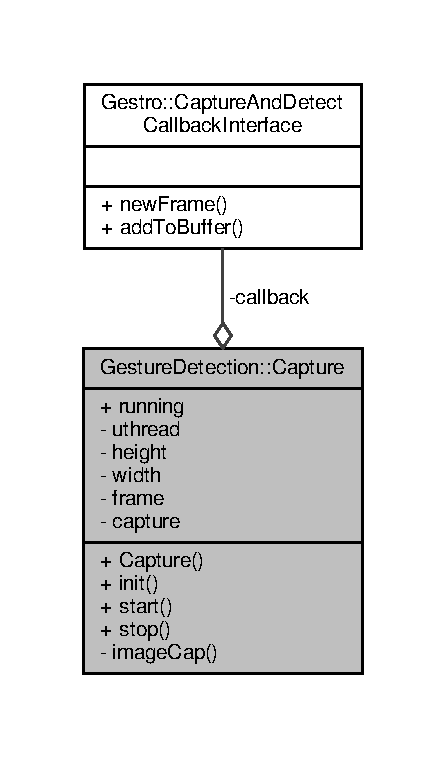
\includegraphics[width=214pt]{class_gesture_detection_1_1_capture__coll__graph}
\end{center}
\end{figure}
\subsection*{Public Member Functions}
\begin{DoxyCompactItemize}
\item 
\hyperlink{class_gesture_detection_1_1_capture_a97036b5d271238bd4852da79a0091b57}{Capture} ()
\item 
void \hyperlink{class_gesture_detection_1_1_capture_aaff420636b6bac6593789344cc990580}{init} (\hyperlink{class_gestro_1_1_capture_and_detect_callback_interface}{Gestro\+::\+Capture\+And\+Detect\+Callback\+Interface} $\ast$, int, int)
\item 
void \hyperlink{class_gesture_detection_1_1_capture_a2ffe4eeac4caa296f4fcc75cc82c1436}{start} ()
\item 
void \hyperlink{class_gesture_detection_1_1_capture_ab632f1927461a909b18cce71ec96f76d}{stop} ()
\end{DoxyCompactItemize}
\subsection*{Public Attributes}
\begin{DoxyCompactItemize}
\item 
bool \hyperlink{class_gesture_detection_1_1_capture_ab022086194534e994259e0f6de25e350}{running} = false
\begin{DoxyCompactList}\small\item\em boolean to check if cmaera is running \end{DoxyCompactList}\end{DoxyCompactItemize}
\subsection*{Private Member Functions}
\begin{DoxyCompactItemize}
\item 
void \hyperlink{class_gesture_detection_1_1_capture_a010b666cb1482b235f8282867e8f1b97}{image\+Cap} ()
\end{DoxyCompactItemize}
\subsection*{Private Attributes}
\begin{DoxyCompactItemize}
\item 
thread \hyperlink{class_gesture_detection_1_1_capture_a1eb079eb874f1d4246d1f4f33a66f13f}{uthread}
\begin{DoxyCompactList}\small\item\em thread to start image capture \end{DoxyCompactList}\item 
\hyperlink{class_gestro_1_1_capture_and_detect_callback_interface}{Gestro\+::\+Capture\+And\+Detect\+Callback\+Interface} $\ast$ \hyperlink{class_gesture_detection_1_1_capture_a1e3b24bb47bd38304293b13f72e330a0}{callback}
\begin{DoxyCompactList}\small\item\em callback to capture and detect \end{DoxyCompactList}\item 
int \hyperlink{class_gesture_detection_1_1_capture_abcfde50571827b62b1b634b7da10832d}{height}
\begin{DoxyCompactList}\small\item\em resolution height \end{DoxyCompactList}\item 
int \hyperlink{class_gesture_detection_1_1_capture_ad3a6d053234b05f0d5004014f8c74f9f}{width}
\begin{DoxyCompactList}\small\item\em resolution width \end{DoxyCompactList}\item 
Mat \hyperlink{class_gesture_detection_1_1_capture_ae91c88b7342fe1ff305a52d9a7114b55}{frame}
\begin{DoxyCompactList}\small\item\em captured frame \end{DoxyCompactList}\item 
Video\+Capture $\ast$ \hyperlink{class_gesture_detection_1_1_capture_a43fc54a372cf9e8321f0db49315bfbf4}{capture}
\begin{DoxyCompactList}\small\item\em pointer to Video\+Capture \end{DoxyCompactList}\end{DoxyCompactItemize}


\subsection{Detailed Description}
runs a thread to start camera and capture image 

A class that captures images from the webcam and calls the callback function with the image. 

Definition at line 18 of file Capture.\+h.



\subsection{Constructor \& Destructor Documentation}
\mbox{\Hypertarget{class_gesture_detection_1_1_capture_a97036b5d271238bd4852da79a0091b57}\label{class_gesture_detection_1_1_capture_a97036b5d271238bd4852da79a0091b57}} 
\index{Gesture\+Detection\+::\+Capture@{Gesture\+Detection\+::\+Capture}!Capture@{Capture}}
\index{Capture@{Capture}!Gesture\+Detection\+::\+Capture@{Gesture\+Detection\+::\+Capture}}
\subsubsection{\texorpdfstring{Capture()}{Capture()}}
{\footnotesize\ttfamily Capture\+::\+Capture (\begin{DoxyParamCaption}{ }\end{DoxyParamCaption})}

The constructor for the class. 

Definition at line 3 of file Capture.\+cpp.



\subsection{Member Function Documentation}
\mbox{\Hypertarget{class_gesture_detection_1_1_capture_a010b666cb1482b235f8282867e8f1b97}\label{class_gesture_detection_1_1_capture_a010b666cb1482b235f8282867e8f1b97}} 
\index{Gesture\+Detection\+::\+Capture@{Gesture\+Detection\+::\+Capture}!image\+Cap@{image\+Cap}}
\index{image\+Cap@{image\+Cap}!Gesture\+Detection\+::\+Capture@{Gesture\+Detection\+::\+Capture}}
\subsubsection{\texorpdfstring{image\+Cap()}{imageCap()}}
{\footnotesize\ttfamily void Capture\+::image\+Cap (\begin{DoxyParamCaption}{ }\end{DoxyParamCaption})\hspace{0.3cm}{\ttfamily [private]}}

It captures an image from the webcam, and then calls the callback function with the image 

Definition at line 32 of file Capture.\+cpp.

Here is the call graph for this function\+:
\nopagebreak
\begin{figure}[H]
\begin{center}
\leavevmode
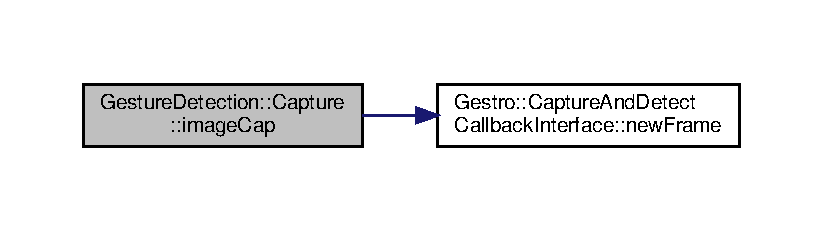
\includegraphics[width=350pt]{class_gesture_detection_1_1_capture_a010b666cb1482b235f8282867e8f1b97_cgraph}
\end{center}
\end{figure}
Here is the caller graph for this function\+:
\nopagebreak
\begin{figure}[H]
\begin{center}
\leavevmode
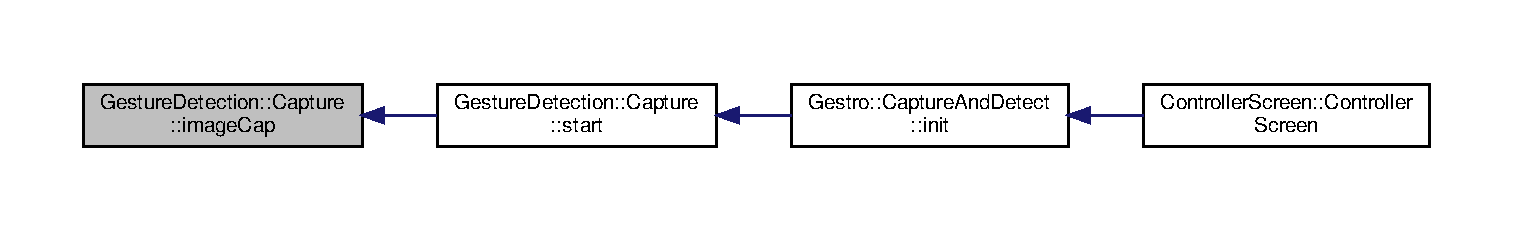
\includegraphics[width=350pt]{class_gesture_detection_1_1_capture_a010b666cb1482b235f8282867e8f1b97_icgraph}
\end{center}
\end{figure}
\mbox{\Hypertarget{class_gesture_detection_1_1_capture_aaff420636b6bac6593789344cc990580}\label{class_gesture_detection_1_1_capture_aaff420636b6bac6593789344cc990580}} 
\index{Gesture\+Detection\+::\+Capture@{Gesture\+Detection\+::\+Capture}!init@{init}}
\index{init@{init}!Gesture\+Detection\+::\+Capture@{Gesture\+Detection\+::\+Capture}}
\subsubsection{\texorpdfstring{init()}{init()}}
{\footnotesize\ttfamily void Capture\+::init (\begin{DoxyParamCaption}\item[{\hyperlink{class_gestro_1_1_capture_and_detect_callback_interface}{Gestro\+::\+Capture\+And\+Detect\+Callback\+Interface} $\ast$}]{interface,  }\item[{int}]{width,  }\item[{int}]{height }\end{DoxyParamCaption})}

It initializes the \hyperlink{class_gesture_detection_1_1_capture}{Capture} class with the width and height of the image to be captured, and a pointer to the Detect\+Interface class


\begin{DoxyParams}{Parameters}
{\em interface} & The interface that will be called when a new frame is available. \\
\hline
{\em width} & The width of the image to be captured. \\
\hline
{\em height} & The height of the image to be captured. \\
\hline
\end{DoxyParams}


Definition at line 5 of file Capture.\+cpp.

Here is the call graph for this function\+:
\nopagebreak
\begin{figure}[H]
\begin{center}
\leavevmode
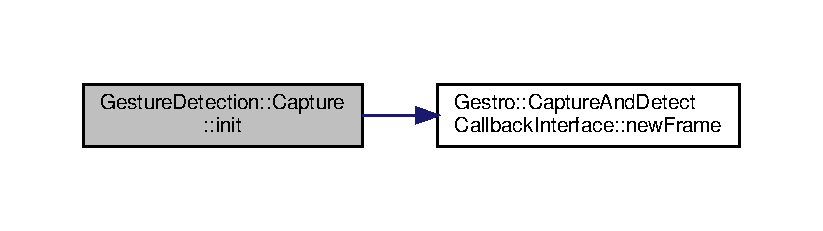
\includegraphics[width=350pt]{class_gesture_detection_1_1_capture_aaff420636b6bac6593789344cc990580_cgraph}
\end{center}
\end{figure}
Here is the caller graph for this function\+:
\nopagebreak
\begin{figure}[H]
\begin{center}
\leavevmode
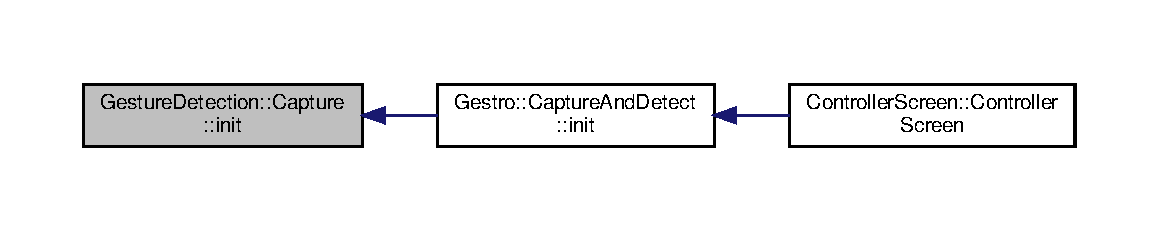
\includegraphics[width=350pt]{class_gesture_detection_1_1_capture_aaff420636b6bac6593789344cc990580_icgraph}
\end{center}
\end{figure}
\mbox{\Hypertarget{class_gesture_detection_1_1_capture_a2ffe4eeac4caa296f4fcc75cc82c1436}\label{class_gesture_detection_1_1_capture_a2ffe4eeac4caa296f4fcc75cc82c1436}} 
\index{Gesture\+Detection\+::\+Capture@{Gesture\+Detection\+::\+Capture}!start@{start}}
\index{start@{start}!Gesture\+Detection\+::\+Capture@{Gesture\+Detection\+::\+Capture}}
\subsubsection{\texorpdfstring{start()}{start()}}
{\footnotesize\ttfamily void Capture\+::start (\begin{DoxyParamCaption}{ }\end{DoxyParamCaption})}

It starts a thread that runs the image\+Cap function to read Images 

Definition at line 22 of file Capture.\+cpp.

Here is the call graph for this function\+:
\nopagebreak
\begin{figure}[H]
\begin{center}
\leavevmode
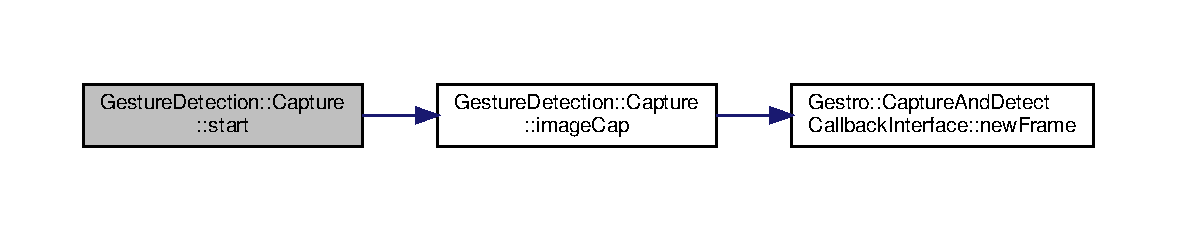
\includegraphics[width=350pt]{class_gesture_detection_1_1_capture_a2ffe4eeac4caa296f4fcc75cc82c1436_cgraph}
\end{center}
\end{figure}
Here is the caller graph for this function\+:
\nopagebreak
\begin{figure}[H]
\begin{center}
\leavevmode
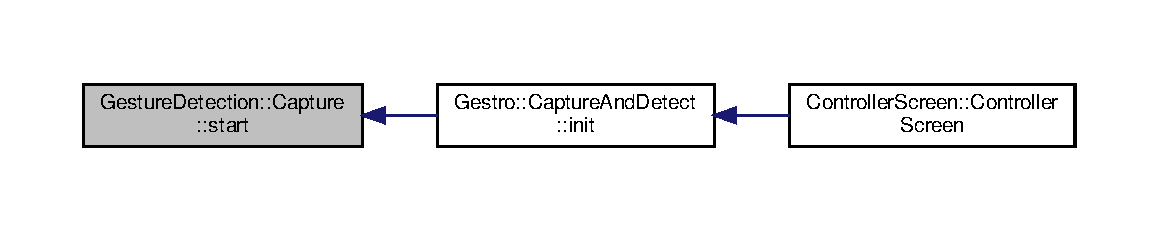
\includegraphics[width=350pt]{class_gesture_detection_1_1_capture_a2ffe4eeac4caa296f4fcc75cc82c1436_icgraph}
\end{center}
\end{figure}
\mbox{\Hypertarget{class_gesture_detection_1_1_capture_ab632f1927461a909b18cce71ec96f76d}\label{class_gesture_detection_1_1_capture_ab632f1927461a909b18cce71ec96f76d}} 
\index{Gesture\+Detection\+::\+Capture@{Gesture\+Detection\+::\+Capture}!stop@{stop}}
\index{stop@{stop}!Gesture\+Detection\+::\+Capture@{Gesture\+Detection\+::\+Capture}}
\subsubsection{\texorpdfstring{stop()}{stop()}}
{\footnotesize\ttfamily void Capture\+::stop (\begin{DoxyParamCaption}{ }\end{DoxyParamCaption})}

It stops the capture thread by setting the running flag to false, and then waits for the thread to finish 

Definition at line 27 of file Capture.\+cpp.



\subsection{Member Data Documentation}
\mbox{\Hypertarget{class_gesture_detection_1_1_capture_a1e3b24bb47bd38304293b13f72e330a0}\label{class_gesture_detection_1_1_capture_a1e3b24bb47bd38304293b13f72e330a0}} 
\index{Gesture\+Detection\+::\+Capture@{Gesture\+Detection\+::\+Capture}!callback@{callback}}
\index{callback@{callback}!Gesture\+Detection\+::\+Capture@{Gesture\+Detection\+::\+Capture}}
\subsubsection{\texorpdfstring{callback}{callback}}
{\footnotesize\ttfamily \hyperlink{class_gestro_1_1_capture_and_detect_callback_interface}{Gestro\+::\+Capture\+And\+Detect\+Callback\+Interface}$\ast$ Gesture\+Detection\+::\+Capture\+::callback\hspace{0.3cm}{\ttfamily [private]}}



callback to capture and detect 



Definition at line 55 of file Capture.\+h.

\mbox{\Hypertarget{class_gesture_detection_1_1_capture_a43fc54a372cf9e8321f0db49315bfbf4}\label{class_gesture_detection_1_1_capture_a43fc54a372cf9e8321f0db49315bfbf4}} 
\index{Gesture\+Detection\+::\+Capture@{Gesture\+Detection\+::\+Capture}!capture@{capture}}
\index{capture@{capture}!Gesture\+Detection\+::\+Capture@{Gesture\+Detection\+::\+Capture}}
\subsubsection{\texorpdfstring{capture}{capture}}
{\footnotesize\ttfamily Video\+Capture$\ast$ Gesture\+Detection\+::\+Capture\+::capture\hspace{0.3cm}{\ttfamily [private]}}



pointer to Video\+Capture 



Definition at line 67 of file Capture.\+h.

\mbox{\Hypertarget{class_gesture_detection_1_1_capture_ae91c88b7342fe1ff305a52d9a7114b55}\label{class_gesture_detection_1_1_capture_ae91c88b7342fe1ff305a52d9a7114b55}} 
\index{Gesture\+Detection\+::\+Capture@{Gesture\+Detection\+::\+Capture}!frame@{frame}}
\index{frame@{frame}!Gesture\+Detection\+::\+Capture@{Gesture\+Detection\+::\+Capture}}
\subsubsection{\texorpdfstring{frame}{frame}}
{\footnotesize\ttfamily Mat Gesture\+Detection\+::\+Capture\+::frame\hspace{0.3cm}{\ttfamily [private]}}



captured frame 



Definition at line 64 of file Capture.\+h.

\mbox{\Hypertarget{class_gesture_detection_1_1_capture_abcfde50571827b62b1b634b7da10832d}\label{class_gesture_detection_1_1_capture_abcfde50571827b62b1b634b7da10832d}} 
\index{Gesture\+Detection\+::\+Capture@{Gesture\+Detection\+::\+Capture}!height@{height}}
\index{height@{height}!Gesture\+Detection\+::\+Capture@{Gesture\+Detection\+::\+Capture}}
\subsubsection{\texorpdfstring{height}{height}}
{\footnotesize\ttfamily int Gesture\+Detection\+::\+Capture\+::height\hspace{0.3cm}{\ttfamily [private]}}



resolution height 



Definition at line 58 of file Capture.\+h.

\mbox{\Hypertarget{class_gesture_detection_1_1_capture_ab022086194534e994259e0f6de25e350}\label{class_gesture_detection_1_1_capture_ab022086194534e994259e0f6de25e350}} 
\index{Gesture\+Detection\+::\+Capture@{Gesture\+Detection\+::\+Capture}!running@{running}}
\index{running@{running}!Gesture\+Detection\+::\+Capture@{Gesture\+Detection\+::\+Capture}}
\subsubsection{\texorpdfstring{running}{running}}
{\footnotesize\ttfamily bool Gesture\+Detection\+::\+Capture\+::running = false}



boolean to check if cmaera is running 



Definition at line 22 of file Capture.\+h.

\mbox{\Hypertarget{class_gesture_detection_1_1_capture_a1eb079eb874f1d4246d1f4f33a66f13f}\label{class_gesture_detection_1_1_capture_a1eb079eb874f1d4246d1f4f33a66f13f}} 
\index{Gesture\+Detection\+::\+Capture@{Gesture\+Detection\+::\+Capture}!uthread@{uthread}}
\index{uthread@{uthread}!Gesture\+Detection\+::\+Capture@{Gesture\+Detection\+::\+Capture}}
\subsubsection{\texorpdfstring{uthread}{uthread}}
{\footnotesize\ttfamily thread Gesture\+Detection\+::\+Capture\+::uthread\hspace{0.3cm}{\ttfamily [private]}}



thread to start image capture 



Definition at line 52 of file Capture.\+h.

\mbox{\Hypertarget{class_gesture_detection_1_1_capture_ad3a6d053234b05f0d5004014f8c74f9f}\label{class_gesture_detection_1_1_capture_ad3a6d053234b05f0d5004014f8c74f9f}} 
\index{Gesture\+Detection\+::\+Capture@{Gesture\+Detection\+::\+Capture}!width@{width}}
\index{width@{width}!Gesture\+Detection\+::\+Capture@{Gesture\+Detection\+::\+Capture}}
\subsubsection{\texorpdfstring{width}{width}}
{\footnotesize\ttfamily int Gesture\+Detection\+::\+Capture\+::width\hspace{0.3cm}{\ttfamily [private]}}



resolution width 



Definition at line 61 of file Capture.\+h.



The documentation for this class was generated from the following files\+:\begin{DoxyCompactItemize}
\item 
src/gesture\+\_\+detection/\hyperlink{_capture_8h}{Capture.\+h}\item 
src/gesture\+\_\+detection/\hyperlink{_capture_8cpp}{Capture.\+cpp}\end{DoxyCompactItemize}

\hypertarget{class_gestro_1_1_capture_and_detect}{}\section{Gestro\+:\+:Capture\+And\+Detect Class Reference}
\label{class_gestro_1_1_capture_and_detect}\index{Gestro\+::\+Capture\+And\+Detect@{Gestro\+::\+Capture\+And\+Detect}}


This class takes care of starting threads to capture image, process and publish commands.  




{\ttfamily \#include $<$Capture\+And\+Detect.\+h$>$}



Inheritance diagram for Gestro\+:\+:Capture\+And\+Detect\+:
\nopagebreak
\begin{figure}[H]
\begin{center}
\leavevmode
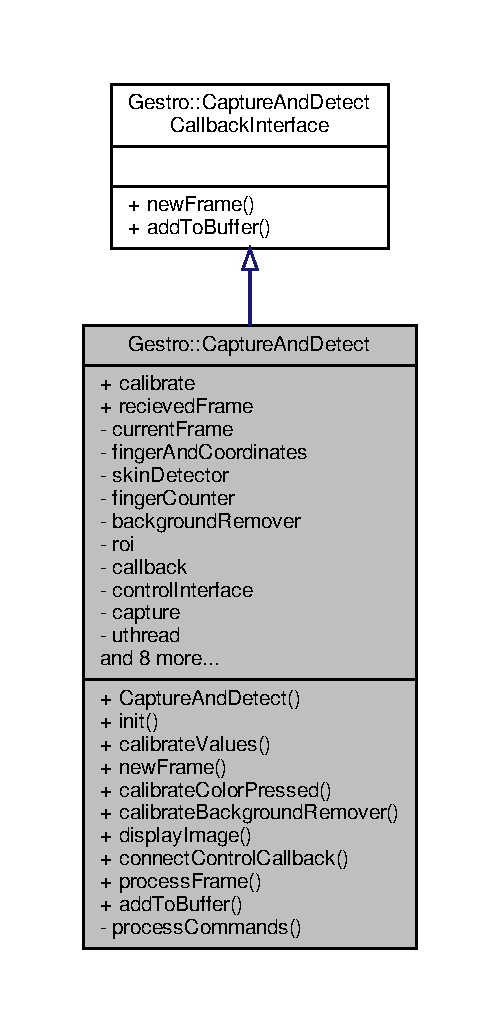
\includegraphics[width=240pt]{class_gestro_1_1_capture_and_detect__inherit__graph}
\end{center}
\end{figure}


Collaboration diagram for Gestro\+:\+:Capture\+And\+Detect\+:
\nopagebreak
\begin{figure}[H]
\begin{center}
\leavevmode
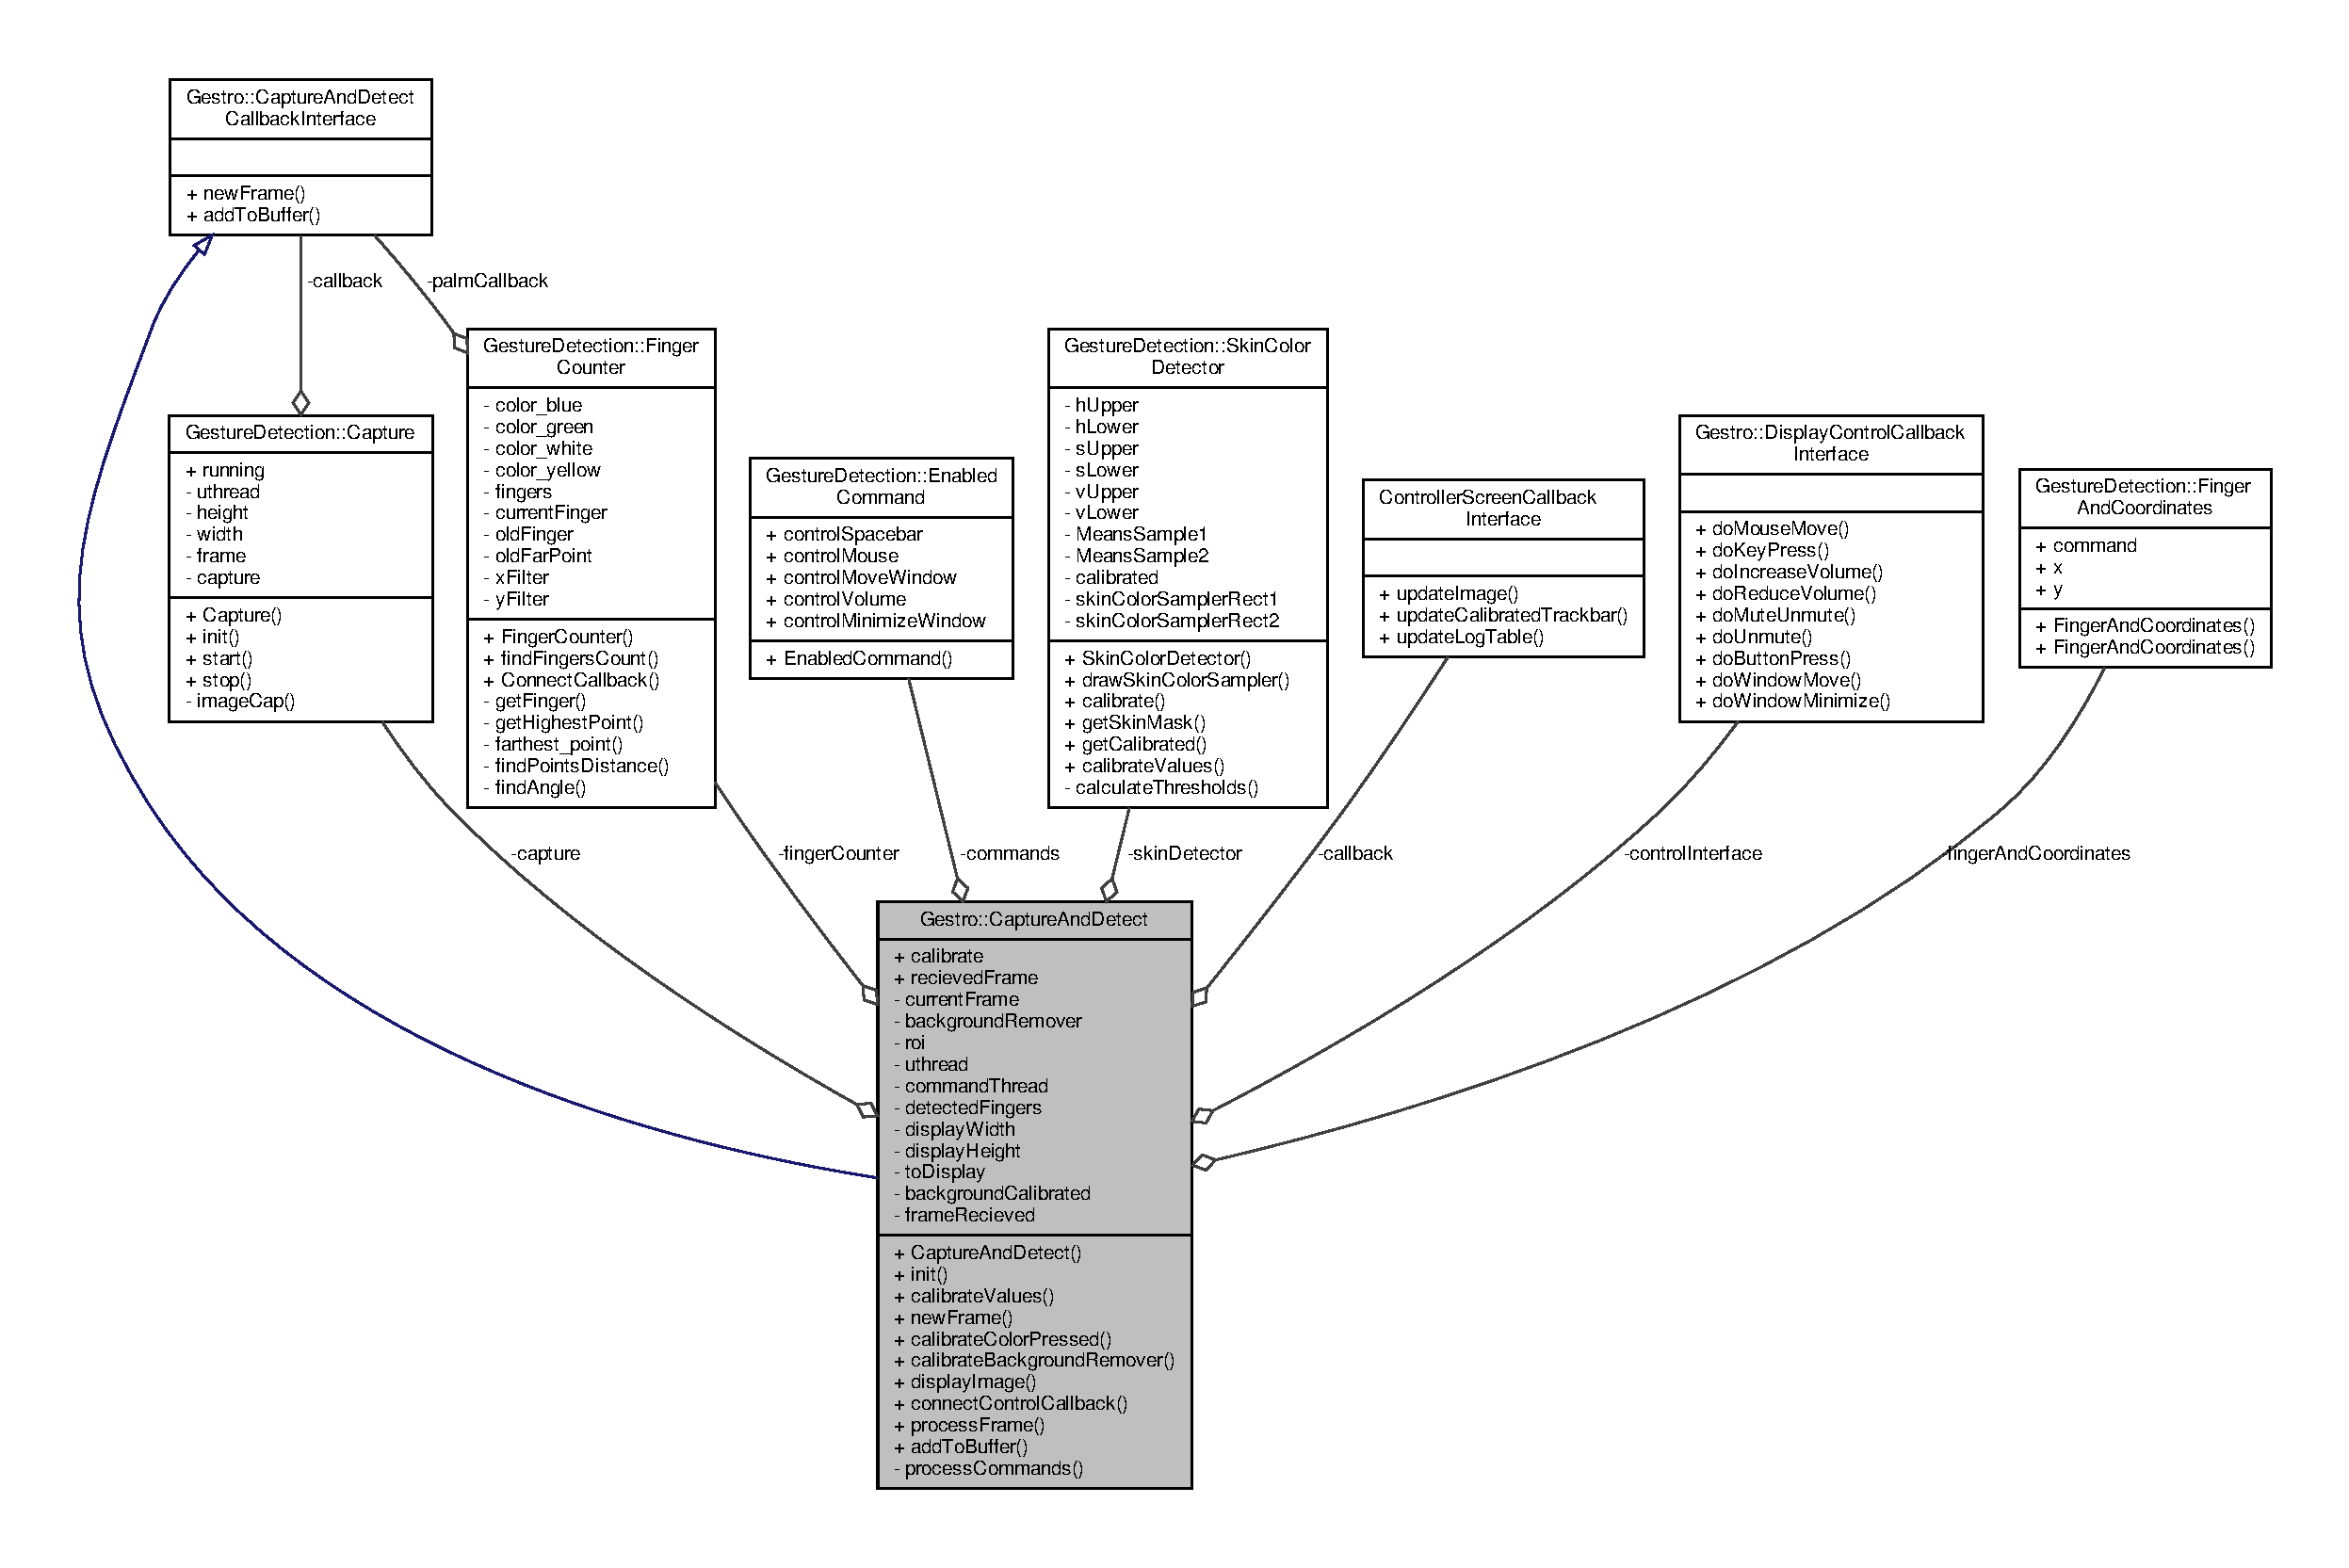
\includegraphics[width=350pt]{class_gestro_1_1_capture_and_detect__coll__graph}
\end{center}
\end{figure}
\subsection*{Public Member Functions}
\begin{DoxyCompactItemize}
\item 
\hyperlink{class_gestro_1_1_capture_and_detect_a26c41eaa5100975ec0f50c97592f4bf1}{Capture\+And\+Detect} ()
\item 
void \hyperlink{class_gestro_1_1_capture_and_detect_a1df110dc696cebc95eb5d7ead2d74447}{init} (\hyperlink{class_controller_screen_callback_interface}{Controller\+Screen\+Callback\+Interface} $\ast$, int, int, \hyperlink{class_gesture_detection_1_1_enabled_command}{Enabled\+Command} $\ast$, \hyperlink{_capture_and_detect_8h_a3c1fc1369ee351f25804c8cde5e85ac3}{Resolution} width=\hyperlink{_capture_and_detect_8h_a3c1fc1369ee351f25804c8cde5e85ac3a278580710dc7c233b4035c222f100b9f}{W\+I\+D\+T\+H\+\_\+1280}, \hyperlink{_capture_and_detect_8h_a3c1fc1369ee351f25804c8cde5e85ac3}{Resolution} height=\hyperlink{_capture_and_detect_8h_a3c1fc1369ee351f25804c8cde5e85ac3aaf8940bab7f04c8cd702f61c4d051f27}{H\+E\+I\+G\+H\+T\+\_\+720})
\item 
void \hyperlink{class_gestro_1_1_capture_and_detect_aafb4f601f860dd38f514f6dd29a1d016}{calibrate\+Values} (int, int, int, int)
\item 
void \hyperlink{class_gestro_1_1_capture_and_detect_a7f18d1c58b2ae4241766b36aa27385e9}{new\+Frame} (Mat) override
\item 
void \hyperlink{class_gestro_1_1_capture_and_detect_ac60f9b1d192c043fa9b40c38fc5599e6}{calibrate\+Color\+Pressed} ()
\item 
void \hyperlink{class_gestro_1_1_capture_and_detect_a53065abfb6eed6c074ad4d3370b3f232}{calibrate\+Background\+Remover} ()
\item 
void \hyperlink{class_gestro_1_1_capture_and_detect_a3f1ba69514a2debbc6b2a03e76f31b65}{display\+Image} (int)
\item 
void \hyperlink{class_gestro_1_1_capture_and_detect_aa75e3ba836797d18aa02c72bbf975082}{connect\+Control\+Callback} (\hyperlink{class_gestro_1_1_display_control_callback_interface}{Display\+Control\+Callback\+Interface} $\ast$)
\item 
void \hyperlink{class_gestro_1_1_capture_and_detect_ac7e70bbcade4e0023541c556ee7cb34e}{process\+Frame} ()
\item 
void \hyperlink{class_gestro_1_1_capture_and_detect_af376ab5418f7b235ee181d574da71fd6}{add\+To\+Buffer} (\hyperlink{class_gesture_detection_1_1_finger_and_coordinates}{Finger\+And\+Coordinates}) override
\end{DoxyCompactItemize}
\subsection*{Public Attributes}
\begin{DoxyCompactItemize}
\item 
bool \hyperlink{class_gestro_1_1_capture_and_detect_acbe1ce90cb6a7bad1c94a6be68cc4f0b}{calibrate} = false
\item 
Mat \hyperlink{class_gestro_1_1_capture_and_detect_a5bd3dee8a4b9bffe627b1475a84da4e8}{recieved\+Frame}
\begin{DoxyCompactList}\small\item\em frame received from capture thread \end{DoxyCompactList}\end{DoxyCompactItemize}
\subsection*{Private Member Functions}
\begin{DoxyCompactItemize}
\item 
void \hyperlink{class_gestro_1_1_capture_and_detect_a5747ba4779f2f30b599c5082088841ed}{process\+Commands} ()
\end{DoxyCompactItemize}
\subsection*{Private Attributes}
\begin{DoxyCompactItemize}
\item 
Mat \hyperlink{class_gestro_1_1_capture_and_detect_ab7694fb9dc10f0819f0c59feb123087a}{current\+Frame}
\begin{DoxyCompactList}\small\item\em current frame being processed \end{DoxyCompactList}\item 
\hyperlink{class_gesture_detection_1_1_finger_and_coordinates}{Finger\+And\+Coordinates} \hyperlink{class_gestro_1_1_capture_and_detect_a0eaec358c409bd96ec89bd86c0f4049b}{finger\+And\+Coordinates}
\begin{DoxyCompactList}\small\item\em Fingercoordinate object to store the response. \end{DoxyCompactList}\item 
\hyperlink{class_gesture_detection_1_1_skin_color_detector}{Skin\+Color\+Detector} \hyperlink{class_gestro_1_1_capture_and_detect_a179ec3c7d8c145f5cbe53d72b64fa656}{skin\+Detector}
\begin{DoxyCompactList}\small\item\em Skin\+Color\+Detecter object. \end{DoxyCompactList}\item 
\hyperlink{class_gesture_detection_1_1_finger_counter}{Finger\+Counter} \hyperlink{class_gestro_1_1_capture_and_detect_a06e92344901d2060142711bb9a2368b9}{finger\+Counter}
\begin{DoxyCompactList}\small\item\em Finger\+Counter object. \end{DoxyCompactList}\item 
Ptr$<$ Background\+Subtractor $>$ \hyperlink{class_gestro_1_1_capture_and_detect_a83873f62b771ca924cf39ee7e8e8eb80}{background\+Remover}
\begin{DoxyCompactList}\small\item\em Bacground substractor object. \end{DoxyCompactList}\item 
Rect \hyperlink{class_gestro_1_1_capture_and_detect_a957cb7ba12d74145492f613fe40c2b10}{roi}
\begin{DoxyCompactList}\small\item\em Region of interest to track the fingers. \end{DoxyCompactList}\item 
\hyperlink{class_controller_screen_callback_interface}{Controller\+Screen\+Callback\+Interface} $\ast$ \hyperlink{class_gestro_1_1_capture_and_detect_ab137d75874d927cb28c5c46e29b82e86}{callback}
\begin{DoxyCompactList}\small\item\em callback to controller screen G\+UI \end{DoxyCompactList}\item 
\hyperlink{class_gestro_1_1_display_control_callback_interface}{Display\+Control\+Callback\+Interface} $\ast$ \hyperlink{class_gestro_1_1_capture_and_detect_ab21df2b869f25d82734079877139d7e4}{control\+Interface}
\begin{DoxyCompactList}\small\item\em callback to Display Control to send ubuntu commands \end{DoxyCompactList}\item 
\hyperlink{class_gesture_detection_1_1_capture}{Capture} \hyperlink{class_gestro_1_1_capture_and_detect_a6873c3bb2ab557d3997b39f0de032233}{capture}
\begin{DoxyCompactList}\small\item\em Capture object. \end{DoxyCompactList}\item 
thread \hyperlink{class_gestro_1_1_capture_and_detect_a0c143ab4c3181d7f32da71bb161e8d02}{uthread}
\begin{DoxyCompactList}\small\item\em thread to start processing images \end{DoxyCompactList}\item 
thread \hyperlink{class_gestro_1_1_capture_and_detect_a0c079f5a40fa2b8485331d0392b40c37}{command\+Thread}
\begin{DoxyCompactList}\small\item\em thread to check for commands and forward to \hyperlink{class_gestro_1_1_display_control}{Display\+Control} \end{DoxyCompactList}\item 
queue$<$ \hyperlink{class_gesture_detection_1_1_finger_and_coordinates}{Finger\+And\+Coordinates} $>$ \hyperlink{class_gestro_1_1_capture_and_detect_a7f7e00691a7d60b5de4c481f8c071bf4}{detected\+Fingers}
\begin{DoxyCompactList}\small\item\em buffer to store the finger count, listened by command thread \end{DoxyCompactList}\item 
\hyperlink{class_gesture_detection_1_1_enabled_command}{Enabled\+Command} $\ast$ \hyperlink{class_gestro_1_1_capture_and_detect_ad2be564539d1862efb8c8f633cc97e96}{commands}
\item 
int \hyperlink{class_gestro_1_1_capture_and_detect_a29f516e20c1196a3dbb3ab5ce52f537a}{display\+Width}
\begin{DoxyCompactList}\small\item\em width of the display \end{DoxyCompactList}\item 
int \hyperlink{class_gestro_1_1_capture_and_detect_ada094d9bbdaddd5eab331ad36939ff1f}{display\+Height}
\begin{DoxyCompactList}\small\item\em height of the display \end{DoxyCompactList}\item 
int \hyperlink{class_gestro_1_1_capture_and_detect_aa2e6f7d381e29a541356d3eff6dcb745}{to\+Display} = \hyperlink{_capture_and_detect_8h_a425a93be55e757f5e351ec9d6770c50ea93c33b647b7a4b7299c25e4e6d98ef7e}{U\+N\+P\+R\+O\+C\+E\+S\+S\+ED}
\begin{DoxyCompactList}\small\item\em feed to display \end{DoxyCompactList}\item 
bool \hyperlink{class_gestro_1_1_capture_and_detect_a7050e1a4e0bcf87954d43edb2cce6a3d}{background\+Calibrated} = false
\begin{DoxyCompactList}\small\item\em bool to check is background has been calibrated \end{DoxyCompactList}\item 
bool \hyperlink{class_gestro_1_1_capture_and_detect_a6ff36cce05c030ceda69abd88e557d88}{frame\+Recieved} = false
\begin{DoxyCompactList}\small\item\em boolean flag to check if recieved new frame from Capture \end{DoxyCompactList}\end{DoxyCompactItemize}


\subsection{Detailed Description}
This class takes care of starting threads to capture image, process and publish commands. 

This class is the mediator between the different functions of the application. Connecting between image capturing, G\+UI and and \hyperlink{class_gestro_1_1_display_control}{Display\+Control} to publish the detected commands. 

Definition at line 41 of file Capture\+And\+Detect.\+h.



\subsection{Constructor \& Destructor Documentation}
\mbox{\Hypertarget{class_gestro_1_1_capture_and_detect_a26c41eaa5100975ec0f50c97592f4bf1}\label{class_gestro_1_1_capture_and_detect_a26c41eaa5100975ec0f50c97592f4bf1}} 
\index{Gestro\+::\+Capture\+And\+Detect@{Gestro\+::\+Capture\+And\+Detect}!Capture\+And\+Detect@{Capture\+And\+Detect}}
\index{Capture\+And\+Detect@{Capture\+And\+Detect}!Gestro\+::\+Capture\+And\+Detect@{Gestro\+::\+Capture\+And\+Detect}}
\subsubsection{\texorpdfstring{Capture\+And\+Detect()}{CaptureAndDetect()}}
{\footnotesize\ttfamily Capture\+And\+Detect\+::\+Capture\+And\+Detect (\begin{DoxyParamCaption}{ }\end{DoxyParamCaption})}

The constructor for the \hyperlink{class_gestro_1_1_capture_and_detect}{Capture\+And\+Detect} class. 

Definition at line 5 of file Capture\+And\+Detect.\+cpp.



\subsection{Member Function Documentation}
\mbox{\Hypertarget{class_gestro_1_1_capture_and_detect_af376ab5418f7b235ee181d574da71fd6}\label{class_gestro_1_1_capture_and_detect_af376ab5418f7b235ee181d574da71fd6}} 
\index{Gestro\+::\+Capture\+And\+Detect@{Gestro\+::\+Capture\+And\+Detect}!add\+To\+Buffer@{add\+To\+Buffer}}
\index{add\+To\+Buffer@{add\+To\+Buffer}!Gestro\+::\+Capture\+And\+Detect@{Gestro\+::\+Capture\+And\+Detect}}
\subsubsection{\texorpdfstring{add\+To\+Buffer()}{addToBuffer()}}
{\footnotesize\ttfamily void Capture\+And\+Detect\+::add\+To\+Buffer (\begin{DoxyParamCaption}\item[{\hyperlink{class_gesture_detection_1_1_finger_and_coordinates}{Finger\+And\+Coordinates}}]{finger }\end{DoxyParamCaption})\hspace{0.3cm}{\ttfamily [override]}, {\ttfamily [virtual]}}

It adds a finger to the buffer


\begin{DoxyParams}{Parameters}
{\em finger} & The finger that was detected. \\
\hline
\end{DoxyParams}


Implements \hyperlink{class_gestro_1_1_capture_and_detect_callback_interface_a8397891f6177ba6257e9cc978d9ddd52}{Gestro\+::\+Capture\+And\+Detect\+Callback\+Interface}.



Definition at line 160 of file Capture\+And\+Detect.\+cpp.

\mbox{\Hypertarget{class_gestro_1_1_capture_and_detect_a53065abfb6eed6c074ad4d3370b3f232}\label{class_gestro_1_1_capture_and_detect_a53065abfb6eed6c074ad4d3370b3f232}} 
\index{Gestro\+::\+Capture\+And\+Detect@{Gestro\+::\+Capture\+And\+Detect}!calibrate\+Background\+Remover@{calibrate\+Background\+Remover}}
\index{calibrate\+Background\+Remover@{calibrate\+Background\+Remover}!Gestro\+::\+Capture\+And\+Detect@{Gestro\+::\+Capture\+And\+Detect}}
\subsubsection{\texorpdfstring{calibrate\+Background\+Remover()}{calibrateBackgroundRemover()}}
{\footnotesize\ttfamily void Capture\+And\+Detect\+::calibrate\+Background\+Remover (\begin{DoxyParamCaption}{ }\end{DoxyParamCaption})}

It creates a background remover object that will be used to remove the background from the video frames 

Definition at line 147 of file Capture\+And\+Detect.\+cpp.

\mbox{\Hypertarget{class_gestro_1_1_capture_and_detect_ac60f9b1d192c043fa9b40c38fc5599e6}\label{class_gestro_1_1_capture_and_detect_ac60f9b1d192c043fa9b40c38fc5599e6}} 
\index{Gestro\+::\+Capture\+And\+Detect@{Gestro\+::\+Capture\+And\+Detect}!calibrate\+Color\+Pressed@{calibrate\+Color\+Pressed}}
\index{calibrate\+Color\+Pressed@{calibrate\+Color\+Pressed}!Gestro\+::\+Capture\+And\+Detect@{Gestro\+::\+Capture\+And\+Detect}}
\subsubsection{\texorpdfstring{calibrate\+Color\+Pressed()}{calibrateColorPressed()}}
{\footnotesize\ttfamily void Capture\+And\+Detect\+::calibrate\+Color\+Pressed (\begin{DoxyParamCaption}{ }\end{DoxyParamCaption})}

It calls the calibrate function of the skin\+Detector object, which returns a vector of 4 integers, which are then passed to the callback function update\+Calibrated\+Trackbar, which updates the trackbar values 

Definition at line 142 of file Capture\+And\+Detect.\+cpp.

Here is the call graph for this function\+:
\nopagebreak
\begin{figure}[H]
\begin{center}
\leavevmode
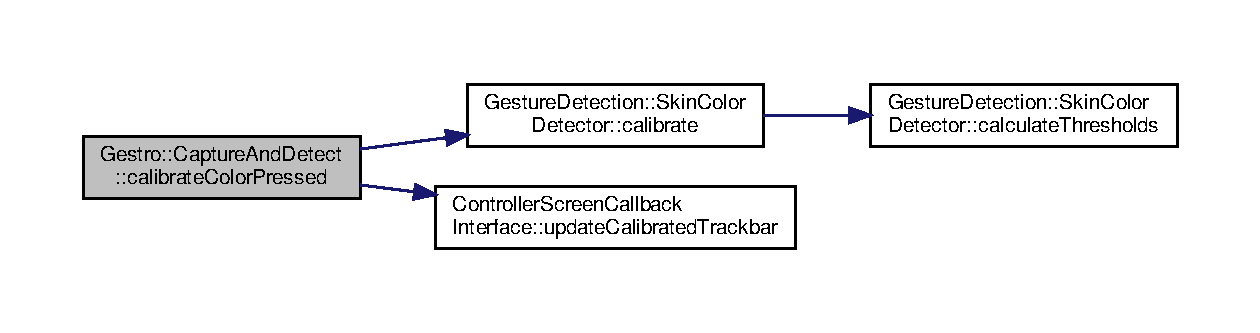
\includegraphics[width=350pt]{class_gestro_1_1_capture_and_detect_ac60f9b1d192c043fa9b40c38fc5599e6_cgraph}
\end{center}
\end{figure}
\mbox{\Hypertarget{class_gestro_1_1_capture_and_detect_aafb4f601f860dd38f514f6dd29a1d016}\label{class_gestro_1_1_capture_and_detect_aafb4f601f860dd38f514f6dd29a1d016}} 
\index{Gestro\+::\+Capture\+And\+Detect@{Gestro\+::\+Capture\+And\+Detect}!calibrate\+Values@{calibrate\+Values}}
\index{calibrate\+Values@{calibrate\+Values}!Gestro\+::\+Capture\+And\+Detect@{Gestro\+::\+Capture\+And\+Detect}}
\subsubsection{\texorpdfstring{calibrate\+Values()}{calibrateValues()}}
{\footnotesize\ttfamily void Capture\+And\+Detect\+::calibrate\+Values (\begin{DoxyParamCaption}\item[{int}]{h\+Min,  }\item[{int}]{h\+Max,  }\item[{int}]{s\+Min,  }\item[{int}]{s\+Max }\end{DoxyParamCaption})}

It takes in the minimum and maximum values for the hue and saturation channels, and then passes them to the skin\+Detector object\textquotesingle{}s \hyperlink{class_gestro_1_1_capture_and_detect_aafb4f601f860dd38f514f6dd29a1d016}{calibrate\+Values()} function


\begin{DoxyParams}{Parameters}
{\em h\+Min} & Minimum Hue value \\
\hline
{\em h\+Max} & The maximum hue value for the skin color. \\
\hline
{\em s\+Min} & Minimum saturation value for the skin color. \\
\hline
{\em s\+Max} & The maximum saturation value for the skin color. \\
\hline
\end{DoxyParams}


Definition at line 22 of file Capture\+And\+Detect.\+cpp.

Here is the call graph for this function\+:
\nopagebreak
\begin{figure}[H]
\begin{center}
\leavevmode
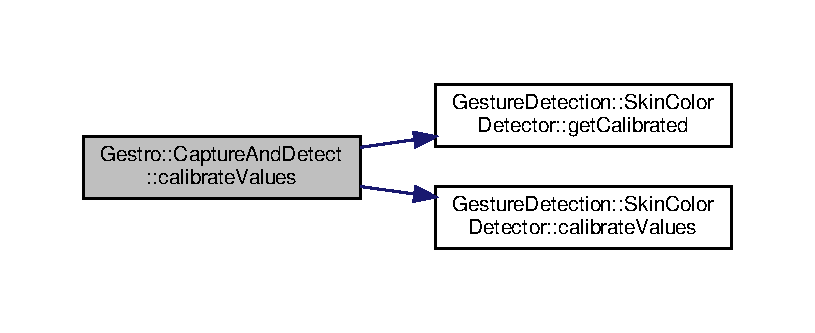
\includegraphics[width=350pt]{class_gestro_1_1_capture_and_detect_aafb4f601f860dd38f514f6dd29a1d016_cgraph}
\end{center}
\end{figure}
\mbox{\Hypertarget{class_gestro_1_1_capture_and_detect_aa75e3ba836797d18aa02c72bbf975082}\label{class_gestro_1_1_capture_and_detect_aa75e3ba836797d18aa02c72bbf975082}} 
\index{Gestro\+::\+Capture\+And\+Detect@{Gestro\+::\+Capture\+And\+Detect}!connect\+Control\+Callback@{connect\+Control\+Callback}}
\index{connect\+Control\+Callback@{connect\+Control\+Callback}!Gestro\+::\+Capture\+And\+Detect@{Gestro\+::\+Capture\+And\+Detect}}
\subsubsection{\texorpdfstring{connect\+Control\+Callback()}{connectControlCallback()}}
{\footnotesize\ttfamily void Capture\+And\+Detect\+::connect\+Control\+Callback (\begin{DoxyParamCaption}\item[{\hyperlink{class_gestro_1_1_display_control_callback_interface}{Display\+Control\+Callback\+Interface} $\ast$}]{interface }\end{DoxyParamCaption})}

This function is called by the \hyperlink{class_gestro_1_1_display_control}{Display\+Control} class to connect the \hyperlink{class_gestro_1_1_capture_and_detect}{Capture\+And\+Detect} class to the \hyperlink{class_gestro_1_1_display_control}{Display\+Control} class.


\begin{DoxyParams}{Parameters}
{\em interface} & The interface that will be used to communicate with the display control. \\
\hline
\end{DoxyParams}


Definition at line 156 of file Capture\+And\+Detect.\+cpp.

Here is the caller graph for this function\+:
\nopagebreak
\begin{figure}[H]
\begin{center}
\leavevmode
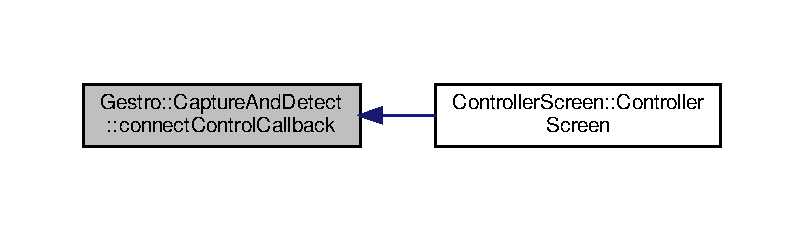
\includegraphics[width=350pt]{class_gestro_1_1_capture_and_detect_aa75e3ba836797d18aa02c72bbf975082_icgraph}
\end{center}
\end{figure}
\mbox{\Hypertarget{class_gestro_1_1_capture_and_detect_a3f1ba69514a2debbc6b2a03e76f31b65}\label{class_gestro_1_1_capture_and_detect_a3f1ba69514a2debbc6b2a03e76f31b65}} 
\index{Gestro\+::\+Capture\+And\+Detect@{Gestro\+::\+Capture\+And\+Detect}!display\+Image@{display\+Image}}
\index{display\+Image@{display\+Image}!Gestro\+::\+Capture\+And\+Detect@{Gestro\+::\+Capture\+And\+Detect}}
\subsubsection{\texorpdfstring{display\+Image()}{displayImage()}}
{\footnotesize\ttfamily void Capture\+And\+Detect\+::display\+Image (\begin{DoxyParamCaption}\item[{int}]{feed }\end{DoxyParamCaption})}

It sets the value of the variable to\+Display to the value of the parameter feed


\begin{DoxyParams}{Parameters}
{\em feed} & The feed to display. \\
\hline
\end{DoxyParams}


Definition at line 152 of file Capture\+And\+Detect.\+cpp.

\mbox{\Hypertarget{class_gestro_1_1_capture_and_detect_a1df110dc696cebc95eb5d7ead2d74447}\label{class_gestro_1_1_capture_and_detect_a1df110dc696cebc95eb5d7ead2d74447}} 
\index{Gestro\+::\+Capture\+And\+Detect@{Gestro\+::\+Capture\+And\+Detect}!init@{init}}
\index{init@{init}!Gestro\+::\+Capture\+And\+Detect@{Gestro\+::\+Capture\+And\+Detect}}
\subsubsection{\texorpdfstring{init()}{init()}}
{\footnotesize\ttfamily void Capture\+And\+Detect\+::init (\begin{DoxyParamCaption}\item[{\hyperlink{class_controller_screen_callback_interface}{Controller\+Screen\+Callback\+Interface} $\ast$}]{interface,  }\item[{int}]{screen\+Width,  }\item[{int}]{screen\+Height,  }\item[{\hyperlink{class_gesture_detection_1_1_enabled_command}{Enabled\+Command} $\ast$}]{enabled\+Command,  }\item[{\hyperlink{_capture_and_detect_8h_a3c1fc1369ee351f25804c8cde5e85ac3}{Resolution}}]{width = {\ttfamily \hyperlink{_capture_and_detect_8h_a3c1fc1369ee351f25804c8cde5e85ac3a278580710dc7c233b4035c222f100b9f}{W\+I\+D\+T\+H\+\_\+1280}},  }\item[{\hyperlink{_capture_and_detect_8h_a3c1fc1369ee351f25804c8cde5e85ac3}{Resolution}}]{height = {\ttfamily \hyperlink{_capture_and_detect_8h_a3c1fc1369ee351f25804c8cde5e85ac3aaf8940bab7f04c8cd702f61c4d051f27}{H\+E\+I\+G\+H\+T\+\_\+720}} }\end{DoxyParamCaption})}

It initializes the capture and detection threads, and starts them


\begin{DoxyParams}{Parameters}
{\em interface} & The interface to call when a gesture is detected. \\
\hline
{\em screen\+Width} & The width of the screen in pixels \\
\hline
{\em screen\+Height} & The height of the screen in pixels \\
\hline
{\em enabled\+Command} & This is a pointer to an Enabled\+Command object. This object is used to determine if the user has enabled the finger counter. \\
\hline
{\em width} & The width of the camera image \\
\hline
{\em height} & The height of the camera\textquotesingle{}s resolution. \\
\hline
\end{DoxyParams}


Definition at line 8 of file Capture\+And\+Detect.\+cpp.

Here is the call graph for this function\+:
\nopagebreak
\begin{figure}[H]
\begin{center}
\leavevmode
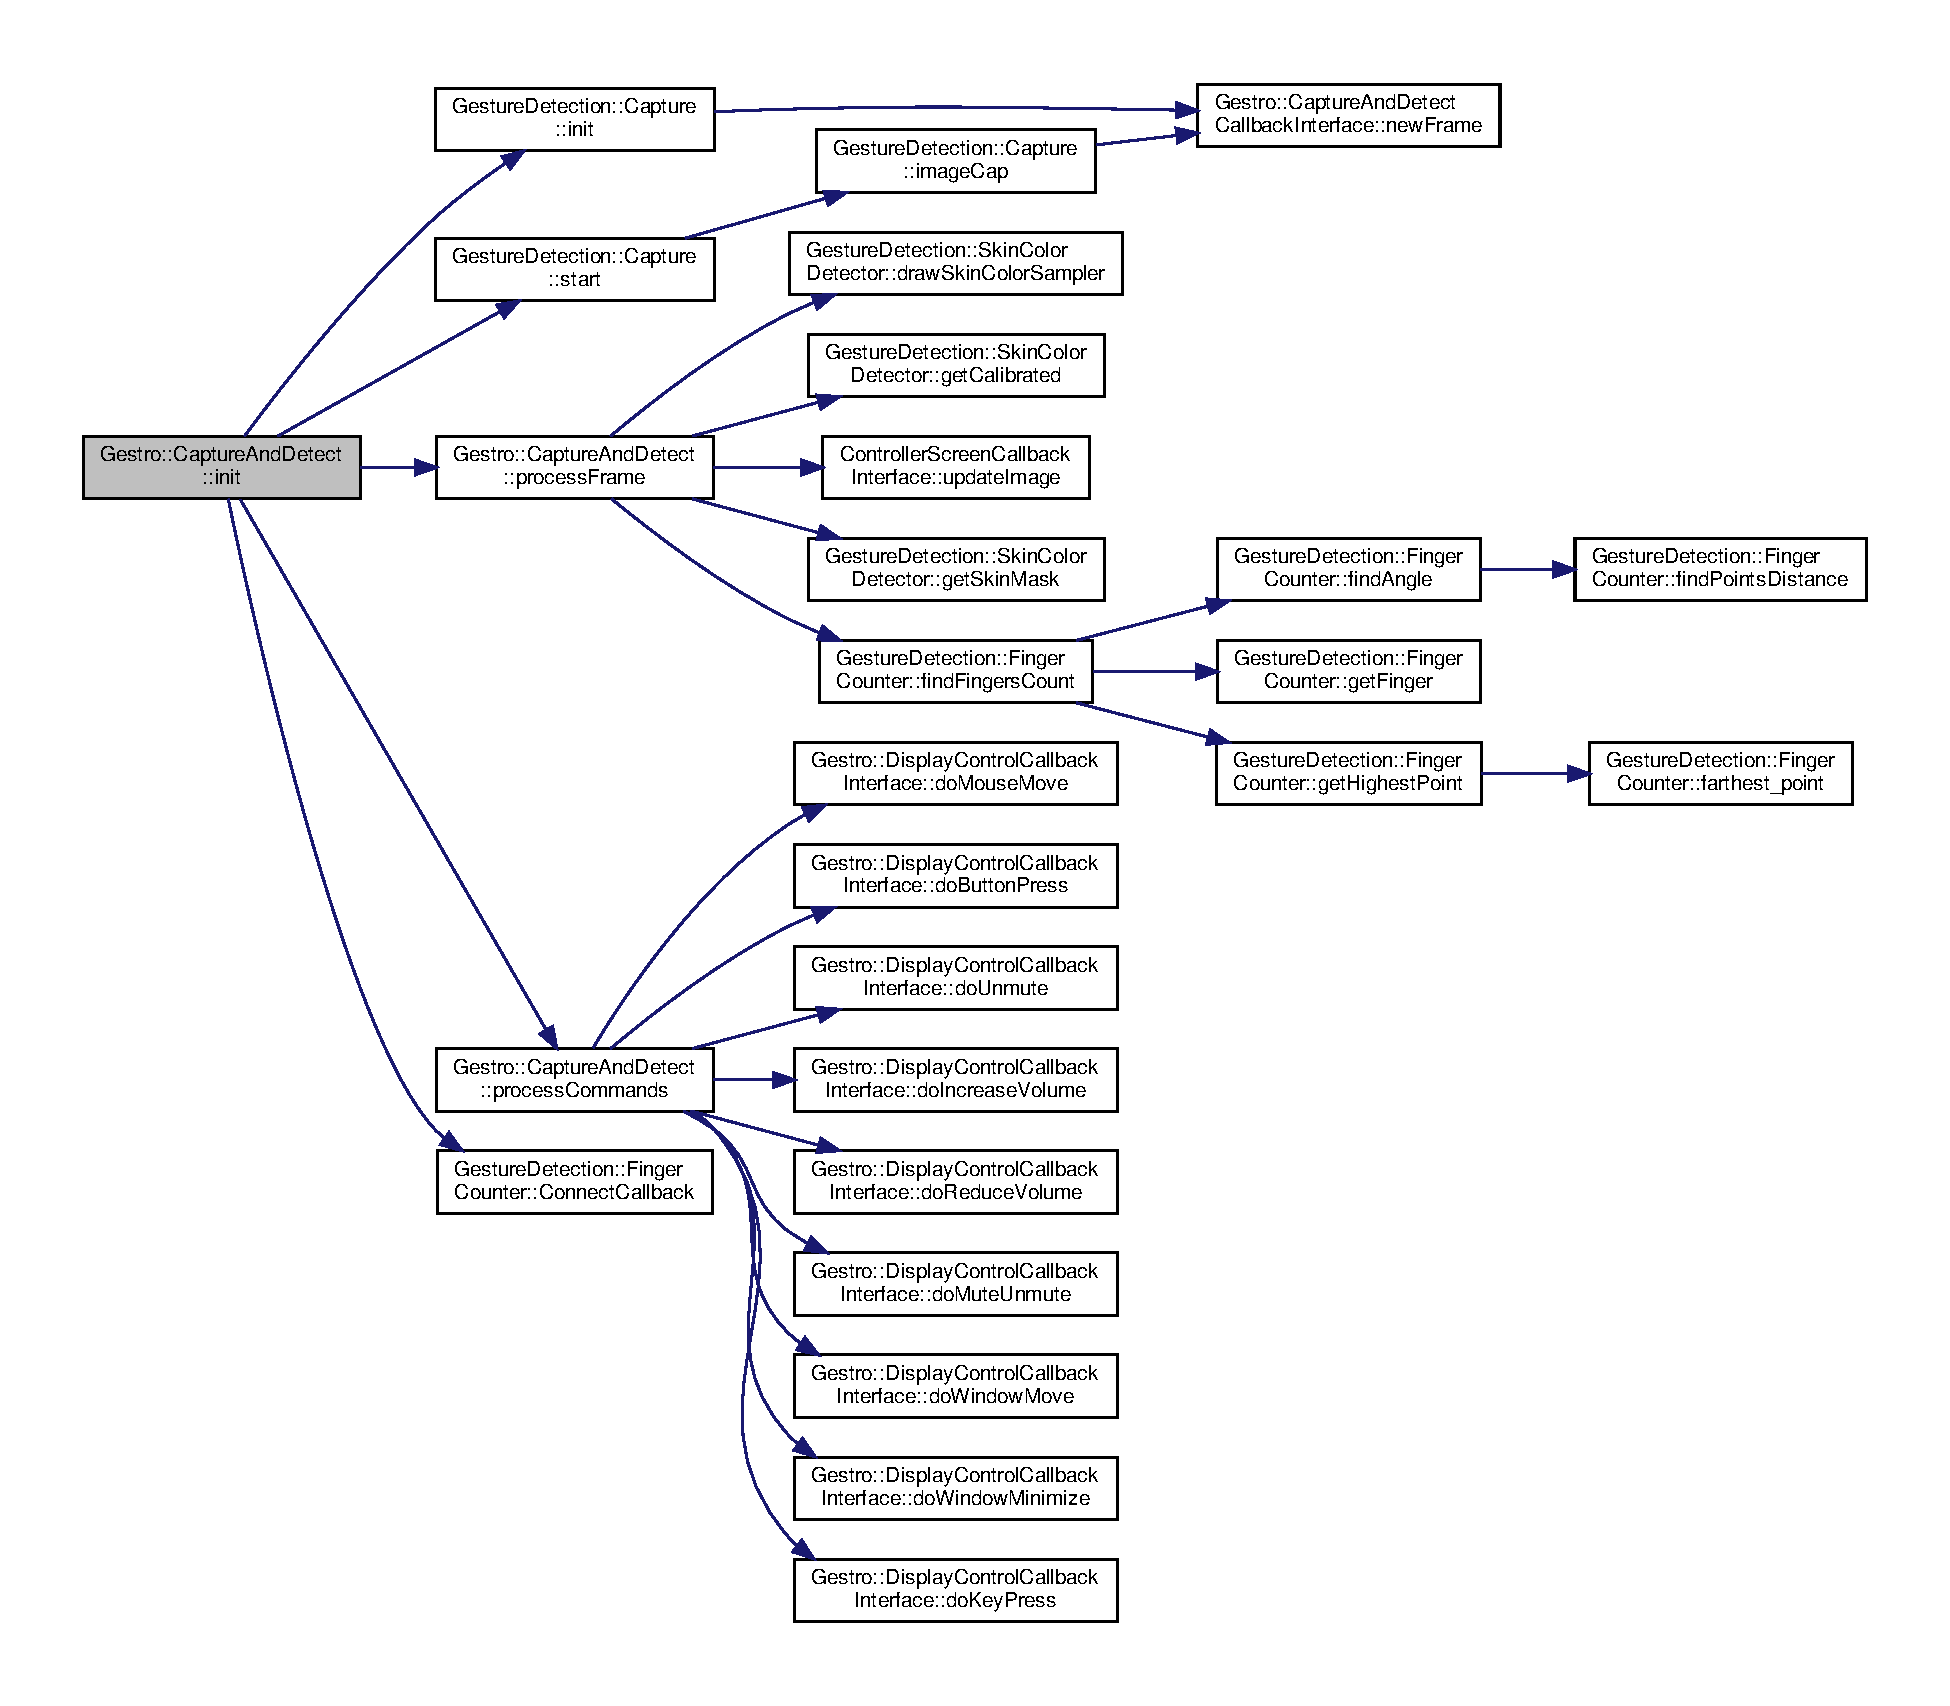
\includegraphics[width=350pt]{class_gestro_1_1_capture_and_detect_a1df110dc696cebc95eb5d7ead2d74447_cgraph}
\end{center}
\end{figure}
Here is the caller graph for this function\+:
\nopagebreak
\begin{figure}[H]
\begin{center}
\leavevmode
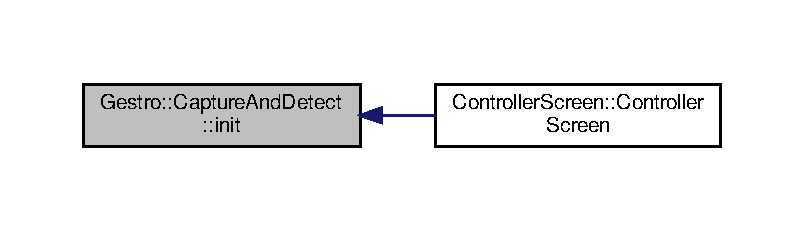
\includegraphics[width=350pt]{class_gestro_1_1_capture_and_detect_a1df110dc696cebc95eb5d7ead2d74447_icgraph}
\end{center}
\end{figure}
\mbox{\Hypertarget{class_gestro_1_1_capture_and_detect_a7f18d1c58b2ae4241766b36aa27385e9}\label{class_gestro_1_1_capture_and_detect_a7f18d1c58b2ae4241766b36aa27385e9}} 
\index{Gestro\+::\+Capture\+And\+Detect@{Gestro\+::\+Capture\+And\+Detect}!new\+Frame@{new\+Frame}}
\index{new\+Frame@{new\+Frame}!Gestro\+::\+Capture\+And\+Detect@{Gestro\+::\+Capture\+And\+Detect}}
\subsubsection{\texorpdfstring{new\+Frame()}{newFrame()}}
{\footnotesize\ttfamily void Capture\+And\+Detect\+::new\+Frame (\begin{DoxyParamCaption}\item[{Mat}]{incoming\+Frame }\end{DoxyParamCaption})\hspace{0.3cm}{\ttfamily [override]}, {\ttfamily [virtual]}}

This function is called by the camera thread when a new frame is available. It sets the recieved\+Frame variable to the new frame and sets the frame\+Recieved variable to true.


\begin{DoxyParams}{Parameters}
{\em incoming\+Frame} & The frame that was recieved from the camera. \\
\hline
\end{DoxyParams}


Implements \hyperlink{class_gestro_1_1_capture_and_detect_callback_interface_a9a42d0f1b3fd64cea607eeb4e6a46287}{Gestro\+::\+Capture\+And\+Detect\+Callback\+Interface}.



Definition at line 29 of file Capture\+And\+Detect.\+cpp.

\mbox{\Hypertarget{class_gestro_1_1_capture_and_detect_a5747ba4779f2f30b599c5082088841ed}\label{class_gestro_1_1_capture_and_detect_a5747ba4779f2f30b599c5082088841ed}} 
\index{Gestro\+::\+Capture\+And\+Detect@{Gestro\+::\+Capture\+And\+Detect}!process\+Commands@{process\+Commands}}
\index{process\+Commands@{process\+Commands}!Gestro\+::\+Capture\+And\+Detect@{Gestro\+::\+Capture\+And\+Detect}}
\subsubsection{\texorpdfstring{process\+Commands()}{processCommands()}}
{\footnotesize\ttfamily void Capture\+And\+Detect\+::process\+Commands (\begin{DoxyParamCaption}{ }\end{DoxyParamCaption})\hspace{0.3cm}{\ttfamily [private]}}

It takes the commands from the queue and executes them 

Definition at line 86 of file Capture\+And\+Detect.\+cpp.

Here is the call graph for this function\+:
\nopagebreak
\begin{figure}[H]
\begin{center}
\leavevmode
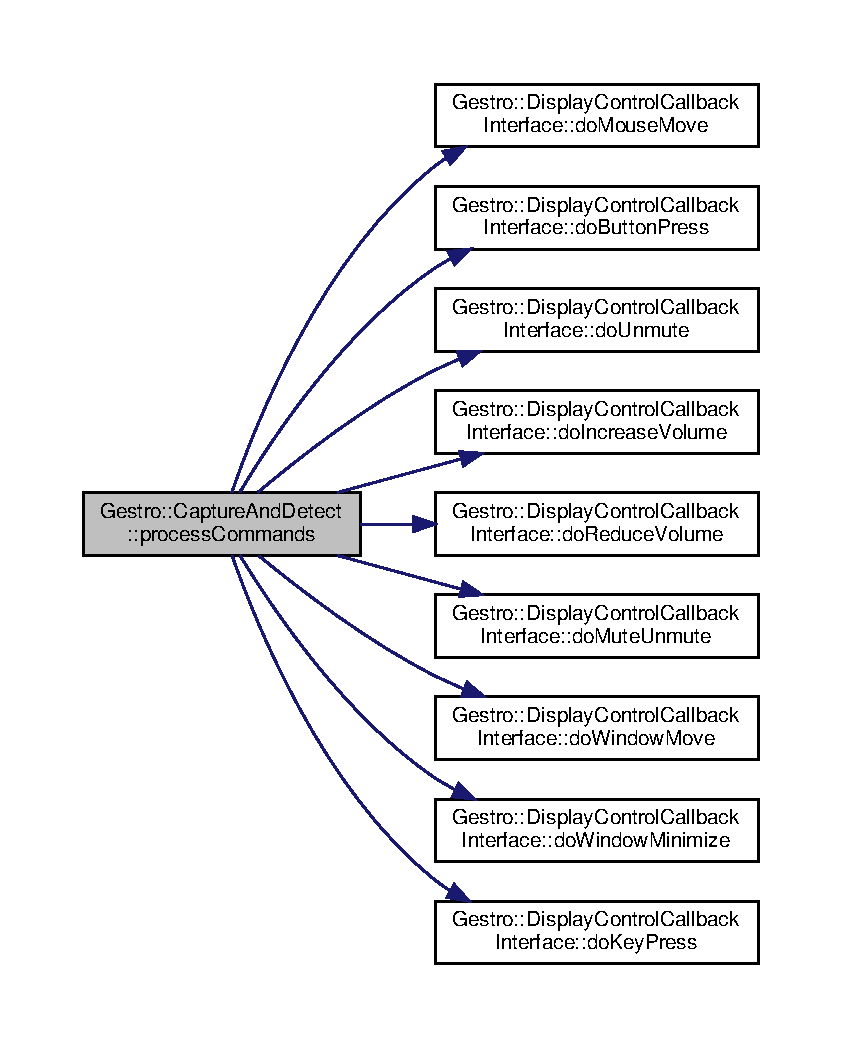
\includegraphics[width=350pt]{class_gestro_1_1_capture_and_detect_a5747ba4779f2f30b599c5082088841ed_cgraph}
\end{center}
\end{figure}
Here is the caller graph for this function\+:
\nopagebreak
\begin{figure}[H]
\begin{center}
\leavevmode
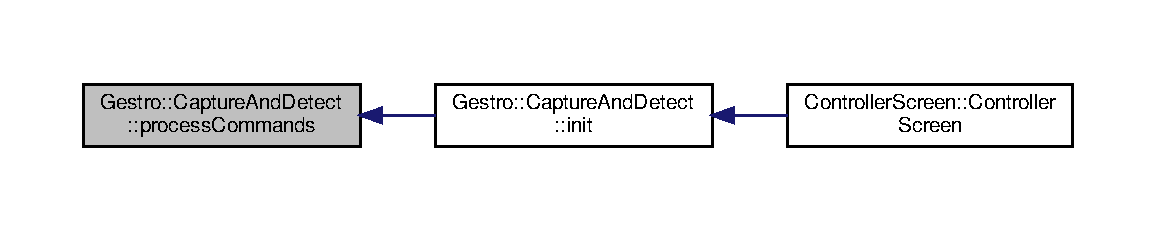
\includegraphics[width=350pt]{class_gestro_1_1_capture_and_detect_a5747ba4779f2f30b599c5082088841ed_icgraph}
\end{center}
\end{figure}
\mbox{\Hypertarget{class_gestro_1_1_capture_and_detect_ac7e70bbcade4e0023541c556ee7cb34e}\label{class_gestro_1_1_capture_and_detect_ac7e70bbcade4e0023541c556ee7cb34e}} 
\index{Gestro\+::\+Capture\+And\+Detect@{Gestro\+::\+Capture\+And\+Detect}!process\+Frame@{process\+Frame}}
\index{process\+Frame@{process\+Frame}!Gestro\+::\+Capture\+And\+Detect@{Gestro\+::\+Capture\+And\+Detect}}
\subsubsection{\texorpdfstring{process\+Frame()}{processFrame()}}
{\footnotesize\ttfamily void Capture\+And\+Detect\+::process\+Frame (\begin{DoxyParamCaption}{ }\end{DoxyParamCaption})}

It takes a frame from the camera, processes it, and sends it to the G\+UI to be displayed 

Definition at line 35 of file Capture\+And\+Detect.\+cpp.

Here is the call graph for this function\+:
\nopagebreak
\begin{figure}[H]
\begin{center}
\leavevmode
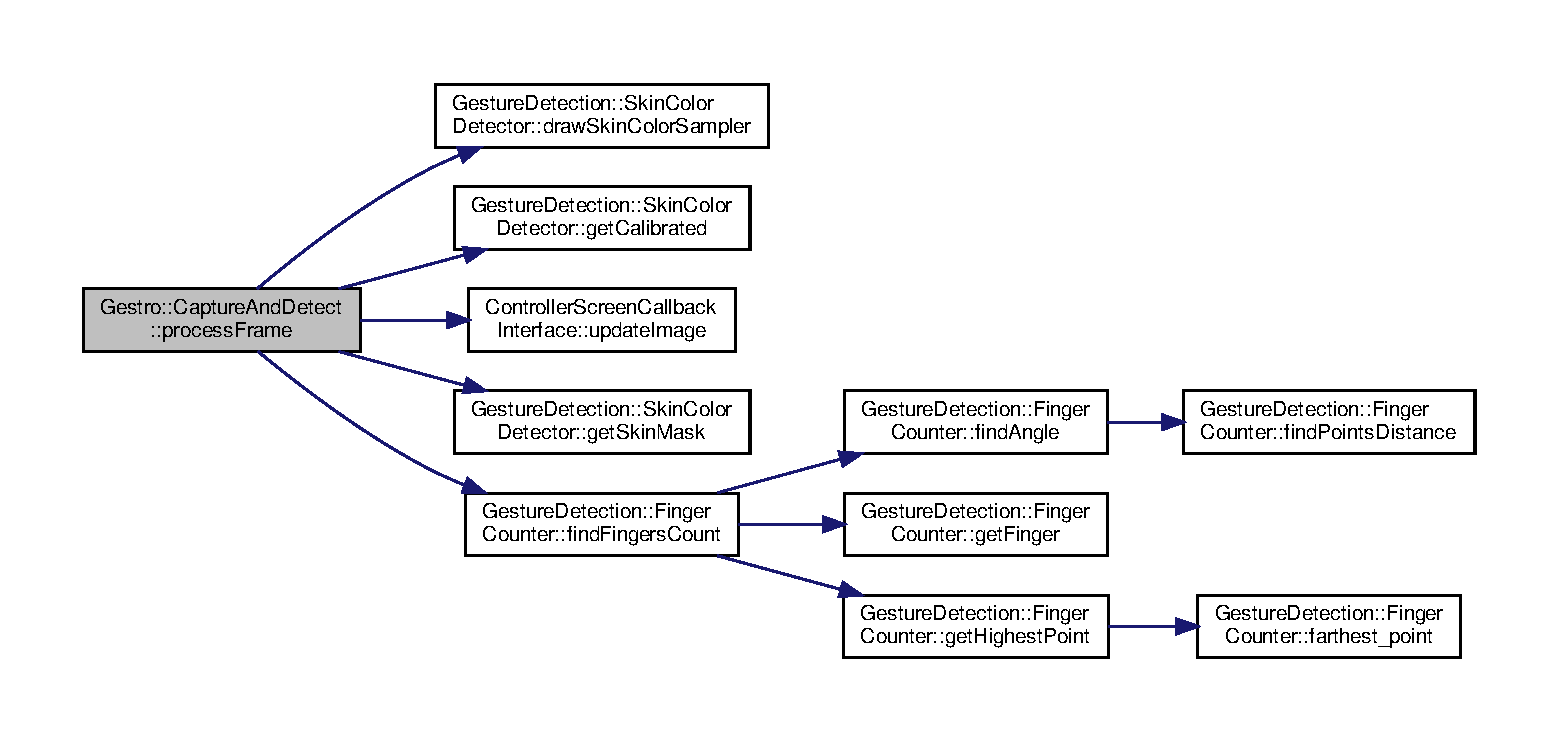
\includegraphics[width=350pt]{class_gestro_1_1_capture_and_detect_ac7e70bbcade4e0023541c556ee7cb34e_cgraph}
\end{center}
\end{figure}
Here is the caller graph for this function\+:
\nopagebreak
\begin{figure}[H]
\begin{center}
\leavevmode
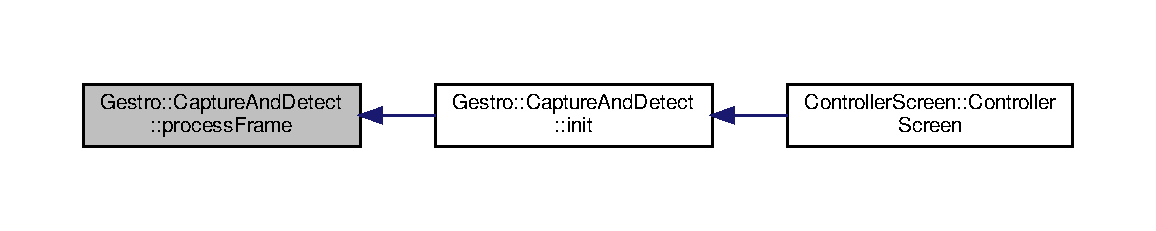
\includegraphics[width=350pt]{class_gestro_1_1_capture_and_detect_ac7e70bbcade4e0023541c556ee7cb34e_icgraph}
\end{center}
\end{figure}


\subsection{Member Data Documentation}
\mbox{\Hypertarget{class_gestro_1_1_capture_and_detect_a7050e1a4e0bcf87954d43edb2cce6a3d}\label{class_gestro_1_1_capture_and_detect_a7050e1a4e0bcf87954d43edb2cce6a3d}} 
\index{Gestro\+::\+Capture\+And\+Detect@{Gestro\+::\+Capture\+And\+Detect}!background\+Calibrated@{background\+Calibrated}}
\index{background\+Calibrated@{background\+Calibrated}!Gestro\+::\+Capture\+And\+Detect@{Gestro\+::\+Capture\+And\+Detect}}
\subsubsection{\texorpdfstring{background\+Calibrated}{backgroundCalibrated}}
{\footnotesize\ttfamily bool Gestro\+::\+Capture\+And\+Detect\+::background\+Calibrated = false\hspace{0.3cm}{\ttfamily [private]}}



bool to check is background has been calibrated 



Definition at line 173 of file Capture\+And\+Detect.\+h.

\mbox{\Hypertarget{class_gestro_1_1_capture_and_detect_a83873f62b771ca924cf39ee7e8e8eb80}\label{class_gestro_1_1_capture_and_detect_a83873f62b771ca924cf39ee7e8e8eb80}} 
\index{Gestro\+::\+Capture\+And\+Detect@{Gestro\+::\+Capture\+And\+Detect}!background\+Remover@{background\+Remover}}
\index{background\+Remover@{background\+Remover}!Gestro\+::\+Capture\+And\+Detect@{Gestro\+::\+Capture\+And\+Detect}}
\subsubsection{\texorpdfstring{background\+Remover}{backgroundRemover}}
{\footnotesize\ttfamily Ptr$<$Background\+Subtractor$>$ Gestro\+::\+Capture\+And\+Detect\+::background\+Remover\hspace{0.3cm}{\ttfamily [private]}}



Bacground substractor object. 



Definition at line 138 of file Capture\+And\+Detect.\+h.

\mbox{\Hypertarget{class_gestro_1_1_capture_and_detect_acbe1ce90cb6a7bad1c94a6be68cc4f0b}\label{class_gestro_1_1_capture_and_detect_acbe1ce90cb6a7bad1c94a6be68cc4f0b}} 
\index{Gestro\+::\+Capture\+And\+Detect@{Gestro\+::\+Capture\+And\+Detect}!calibrate@{calibrate}}
\index{calibrate@{calibrate}!Gestro\+::\+Capture\+And\+Detect@{Gestro\+::\+Capture\+And\+Detect}}
\subsubsection{\texorpdfstring{calibrate}{calibrate}}
{\footnotesize\ttfamily bool Gestro\+::\+Capture\+And\+Detect\+::calibrate = false}



Definition at line 88 of file Capture\+And\+Detect.\+h.

\mbox{\Hypertarget{class_gestro_1_1_capture_and_detect_ab137d75874d927cb28c5c46e29b82e86}\label{class_gestro_1_1_capture_and_detect_ab137d75874d927cb28c5c46e29b82e86}} 
\index{Gestro\+::\+Capture\+And\+Detect@{Gestro\+::\+Capture\+And\+Detect}!callback@{callback}}
\index{callback@{callback}!Gestro\+::\+Capture\+And\+Detect@{Gestro\+::\+Capture\+And\+Detect}}
\subsubsection{\texorpdfstring{callback}{callback}}
{\footnotesize\ttfamily \hyperlink{class_controller_screen_callback_interface}{Controller\+Screen\+Callback\+Interface}$\ast$ Gestro\+::\+Capture\+And\+Detect\+::callback\hspace{0.3cm}{\ttfamily [private]}}



callback to controller screen G\+UI 



Definition at line 144 of file Capture\+And\+Detect.\+h.

\mbox{\Hypertarget{class_gestro_1_1_capture_and_detect_a6873c3bb2ab557d3997b39f0de032233}\label{class_gestro_1_1_capture_and_detect_a6873c3bb2ab557d3997b39f0de032233}} 
\index{Gestro\+::\+Capture\+And\+Detect@{Gestro\+::\+Capture\+And\+Detect}!capture@{capture}}
\index{capture@{capture}!Gestro\+::\+Capture\+And\+Detect@{Gestro\+::\+Capture\+And\+Detect}}
\subsubsection{\texorpdfstring{capture}{capture}}
{\footnotesize\ttfamily \hyperlink{class_gesture_detection_1_1_capture}{Capture} Gestro\+::\+Capture\+And\+Detect\+::capture\hspace{0.3cm}{\ttfamily [private]}}



Capture object. 



Definition at line 150 of file Capture\+And\+Detect.\+h.

\mbox{\Hypertarget{class_gestro_1_1_capture_and_detect_ad2be564539d1862efb8c8f633cc97e96}\label{class_gestro_1_1_capture_and_detect_ad2be564539d1862efb8c8f633cc97e96}} 
\index{Gestro\+::\+Capture\+And\+Detect@{Gestro\+::\+Capture\+And\+Detect}!commands@{commands}}
\index{commands@{commands}!Gestro\+::\+Capture\+And\+Detect@{Gestro\+::\+Capture\+And\+Detect}}
\subsubsection{\texorpdfstring{commands}{commands}}
{\footnotesize\ttfamily \hyperlink{class_gesture_detection_1_1_enabled_command}{Enabled\+Command}$\ast$ Gestro\+::\+Capture\+And\+Detect\+::commands\hspace{0.3cm}{\ttfamily [private]}}



Definition at line 161 of file Capture\+And\+Detect.\+h.

\mbox{\Hypertarget{class_gestro_1_1_capture_and_detect_a0c079f5a40fa2b8485331d0392b40c37}\label{class_gestro_1_1_capture_and_detect_a0c079f5a40fa2b8485331d0392b40c37}} 
\index{Gestro\+::\+Capture\+And\+Detect@{Gestro\+::\+Capture\+And\+Detect}!command\+Thread@{command\+Thread}}
\index{command\+Thread@{command\+Thread}!Gestro\+::\+Capture\+And\+Detect@{Gestro\+::\+Capture\+And\+Detect}}
\subsubsection{\texorpdfstring{command\+Thread}{commandThread}}
{\footnotesize\ttfamily thread Gestro\+::\+Capture\+And\+Detect\+::command\+Thread\hspace{0.3cm}{\ttfamily [private]}}



thread to check for commands and forward to \hyperlink{class_gestro_1_1_display_control}{Display\+Control} 



Definition at line 156 of file Capture\+And\+Detect.\+h.

\mbox{\Hypertarget{class_gestro_1_1_capture_and_detect_ab21df2b869f25d82734079877139d7e4}\label{class_gestro_1_1_capture_and_detect_ab21df2b869f25d82734079877139d7e4}} 
\index{Gestro\+::\+Capture\+And\+Detect@{Gestro\+::\+Capture\+And\+Detect}!control\+Interface@{control\+Interface}}
\index{control\+Interface@{control\+Interface}!Gestro\+::\+Capture\+And\+Detect@{Gestro\+::\+Capture\+And\+Detect}}
\subsubsection{\texorpdfstring{control\+Interface}{controlInterface}}
{\footnotesize\ttfamily \hyperlink{class_gestro_1_1_display_control_callback_interface}{Display\+Control\+Callback\+Interface}$\ast$ Gestro\+::\+Capture\+And\+Detect\+::control\+Interface\hspace{0.3cm}{\ttfamily [private]}}



callback to Display Control to send ubuntu commands 



Definition at line 147 of file Capture\+And\+Detect.\+h.

\mbox{\Hypertarget{class_gestro_1_1_capture_and_detect_ab7694fb9dc10f0819f0c59feb123087a}\label{class_gestro_1_1_capture_and_detect_ab7694fb9dc10f0819f0c59feb123087a}} 
\index{Gestro\+::\+Capture\+And\+Detect@{Gestro\+::\+Capture\+And\+Detect}!current\+Frame@{current\+Frame}}
\index{current\+Frame@{current\+Frame}!Gestro\+::\+Capture\+And\+Detect@{Gestro\+::\+Capture\+And\+Detect}}
\subsubsection{\texorpdfstring{current\+Frame}{currentFrame}}
{\footnotesize\ttfamily Mat Gestro\+::\+Capture\+And\+Detect\+::current\+Frame\hspace{0.3cm}{\ttfamily [private]}}



current frame being processed 



Definition at line 126 of file Capture\+And\+Detect.\+h.

\mbox{\Hypertarget{class_gestro_1_1_capture_and_detect_a7f7e00691a7d60b5de4c481f8c071bf4}\label{class_gestro_1_1_capture_and_detect_a7f7e00691a7d60b5de4c481f8c071bf4}} 
\index{Gestro\+::\+Capture\+And\+Detect@{Gestro\+::\+Capture\+And\+Detect}!detected\+Fingers@{detected\+Fingers}}
\index{detected\+Fingers@{detected\+Fingers}!Gestro\+::\+Capture\+And\+Detect@{Gestro\+::\+Capture\+And\+Detect}}
\subsubsection{\texorpdfstring{detected\+Fingers}{detectedFingers}}
{\footnotesize\ttfamily queue$<$\hyperlink{class_gesture_detection_1_1_finger_and_coordinates}{Finger\+And\+Coordinates}$>$ Gestro\+::\+Capture\+And\+Detect\+::detected\+Fingers\hspace{0.3cm}{\ttfamily [private]}}



buffer to store the finger count, listened by command thread 



Definition at line 159 of file Capture\+And\+Detect.\+h.

\mbox{\Hypertarget{class_gestro_1_1_capture_and_detect_ada094d9bbdaddd5eab331ad36939ff1f}\label{class_gestro_1_1_capture_and_detect_ada094d9bbdaddd5eab331ad36939ff1f}} 
\index{Gestro\+::\+Capture\+And\+Detect@{Gestro\+::\+Capture\+And\+Detect}!display\+Height@{display\+Height}}
\index{display\+Height@{display\+Height}!Gestro\+::\+Capture\+And\+Detect@{Gestro\+::\+Capture\+And\+Detect}}
\subsubsection{\texorpdfstring{display\+Height}{displayHeight}}
{\footnotesize\ttfamily int Gestro\+::\+Capture\+And\+Detect\+::display\+Height\hspace{0.3cm}{\ttfamily [private]}}



height of the display 



Definition at line 167 of file Capture\+And\+Detect.\+h.

\mbox{\Hypertarget{class_gestro_1_1_capture_and_detect_a29f516e20c1196a3dbb3ab5ce52f537a}\label{class_gestro_1_1_capture_and_detect_a29f516e20c1196a3dbb3ab5ce52f537a}} 
\index{Gestro\+::\+Capture\+And\+Detect@{Gestro\+::\+Capture\+And\+Detect}!display\+Width@{display\+Width}}
\index{display\+Width@{display\+Width}!Gestro\+::\+Capture\+And\+Detect@{Gestro\+::\+Capture\+And\+Detect}}
\subsubsection{\texorpdfstring{display\+Width}{displayWidth}}
{\footnotesize\ttfamily int Gestro\+::\+Capture\+And\+Detect\+::display\+Width\hspace{0.3cm}{\ttfamily [private]}}



width of the display 



Definition at line 164 of file Capture\+And\+Detect.\+h.

\mbox{\Hypertarget{class_gestro_1_1_capture_and_detect_a0eaec358c409bd96ec89bd86c0f4049b}\label{class_gestro_1_1_capture_and_detect_a0eaec358c409bd96ec89bd86c0f4049b}} 
\index{Gestro\+::\+Capture\+And\+Detect@{Gestro\+::\+Capture\+And\+Detect}!finger\+And\+Coordinates@{finger\+And\+Coordinates}}
\index{finger\+And\+Coordinates@{finger\+And\+Coordinates}!Gestro\+::\+Capture\+And\+Detect@{Gestro\+::\+Capture\+And\+Detect}}
\subsubsection{\texorpdfstring{finger\+And\+Coordinates}{fingerAndCoordinates}}
{\footnotesize\ttfamily \hyperlink{class_gesture_detection_1_1_finger_and_coordinates}{Finger\+And\+Coordinates} Gestro\+::\+Capture\+And\+Detect\+::finger\+And\+Coordinates\hspace{0.3cm}{\ttfamily [private]}}



Fingercoordinate object to store the response. 



Definition at line 129 of file Capture\+And\+Detect.\+h.

\mbox{\Hypertarget{class_gestro_1_1_capture_and_detect_a06e92344901d2060142711bb9a2368b9}\label{class_gestro_1_1_capture_and_detect_a06e92344901d2060142711bb9a2368b9}} 
\index{Gestro\+::\+Capture\+And\+Detect@{Gestro\+::\+Capture\+And\+Detect}!finger\+Counter@{finger\+Counter}}
\index{finger\+Counter@{finger\+Counter}!Gestro\+::\+Capture\+And\+Detect@{Gestro\+::\+Capture\+And\+Detect}}
\subsubsection{\texorpdfstring{finger\+Counter}{fingerCounter}}
{\footnotesize\ttfamily \hyperlink{class_gesture_detection_1_1_finger_counter}{Finger\+Counter} Gestro\+::\+Capture\+And\+Detect\+::finger\+Counter\hspace{0.3cm}{\ttfamily [private]}}



Finger\+Counter object. 



Definition at line 135 of file Capture\+And\+Detect.\+h.

\mbox{\Hypertarget{class_gestro_1_1_capture_and_detect_a6ff36cce05c030ceda69abd88e557d88}\label{class_gestro_1_1_capture_and_detect_a6ff36cce05c030ceda69abd88e557d88}} 
\index{Gestro\+::\+Capture\+And\+Detect@{Gestro\+::\+Capture\+And\+Detect}!frame\+Recieved@{frame\+Recieved}}
\index{frame\+Recieved@{frame\+Recieved}!Gestro\+::\+Capture\+And\+Detect@{Gestro\+::\+Capture\+And\+Detect}}
\subsubsection{\texorpdfstring{frame\+Recieved}{frameRecieved}}
{\footnotesize\ttfamily bool Gestro\+::\+Capture\+And\+Detect\+::frame\+Recieved = false\hspace{0.3cm}{\ttfamily [private]}}



boolean flag to check if recieved new frame from Capture 



Definition at line 176 of file Capture\+And\+Detect.\+h.

\mbox{\Hypertarget{class_gestro_1_1_capture_and_detect_a5bd3dee8a4b9bffe627b1475a84da4e8}\label{class_gestro_1_1_capture_and_detect_a5bd3dee8a4b9bffe627b1475a84da4e8}} 
\index{Gestro\+::\+Capture\+And\+Detect@{Gestro\+::\+Capture\+And\+Detect}!recieved\+Frame@{recieved\+Frame}}
\index{recieved\+Frame@{recieved\+Frame}!Gestro\+::\+Capture\+And\+Detect@{Gestro\+::\+Capture\+And\+Detect}}
\subsubsection{\texorpdfstring{recieved\+Frame}{recievedFrame}}
{\footnotesize\ttfamily Mat Gestro\+::\+Capture\+And\+Detect\+::recieved\+Frame}



frame received from capture thread 



Definition at line 122 of file Capture\+And\+Detect.\+h.

\mbox{\Hypertarget{class_gestro_1_1_capture_and_detect_a957cb7ba12d74145492f613fe40c2b10}\label{class_gestro_1_1_capture_and_detect_a957cb7ba12d74145492f613fe40c2b10}} 
\index{Gestro\+::\+Capture\+And\+Detect@{Gestro\+::\+Capture\+And\+Detect}!roi@{roi}}
\index{roi@{roi}!Gestro\+::\+Capture\+And\+Detect@{Gestro\+::\+Capture\+And\+Detect}}
\subsubsection{\texorpdfstring{roi}{roi}}
{\footnotesize\ttfamily Rect Gestro\+::\+Capture\+And\+Detect\+::roi\hspace{0.3cm}{\ttfamily [private]}}



Region of interest to track the fingers. 



Definition at line 141 of file Capture\+And\+Detect.\+h.

\mbox{\Hypertarget{class_gestro_1_1_capture_and_detect_a179ec3c7d8c145f5cbe53d72b64fa656}\label{class_gestro_1_1_capture_and_detect_a179ec3c7d8c145f5cbe53d72b64fa656}} 
\index{Gestro\+::\+Capture\+And\+Detect@{Gestro\+::\+Capture\+And\+Detect}!skin\+Detector@{skin\+Detector}}
\index{skin\+Detector@{skin\+Detector}!Gestro\+::\+Capture\+And\+Detect@{Gestro\+::\+Capture\+And\+Detect}}
\subsubsection{\texorpdfstring{skin\+Detector}{skinDetector}}
{\footnotesize\ttfamily \hyperlink{class_gesture_detection_1_1_skin_color_detector}{Skin\+Color\+Detector} Gestro\+::\+Capture\+And\+Detect\+::skin\+Detector\hspace{0.3cm}{\ttfamily [private]}}



Skin\+Color\+Detecter object. 



Definition at line 132 of file Capture\+And\+Detect.\+h.

\mbox{\Hypertarget{class_gestro_1_1_capture_and_detect_aa2e6f7d381e29a541356d3eff6dcb745}\label{class_gestro_1_1_capture_and_detect_aa2e6f7d381e29a541356d3eff6dcb745}} 
\index{Gestro\+::\+Capture\+And\+Detect@{Gestro\+::\+Capture\+And\+Detect}!to\+Display@{to\+Display}}
\index{to\+Display@{to\+Display}!Gestro\+::\+Capture\+And\+Detect@{Gestro\+::\+Capture\+And\+Detect}}
\subsubsection{\texorpdfstring{to\+Display}{toDisplay}}
{\footnotesize\ttfamily int Gestro\+::\+Capture\+And\+Detect\+::to\+Display = \hyperlink{_capture_and_detect_8h_a425a93be55e757f5e351ec9d6770c50ea93c33b647b7a4b7299c25e4e6d98ef7e}{U\+N\+P\+R\+O\+C\+E\+S\+S\+ED}\hspace{0.3cm}{\ttfamily [private]}}



feed to display 



Definition at line 170 of file Capture\+And\+Detect.\+h.

\mbox{\Hypertarget{class_gestro_1_1_capture_and_detect_a0c143ab4c3181d7f32da71bb161e8d02}\label{class_gestro_1_1_capture_and_detect_a0c143ab4c3181d7f32da71bb161e8d02}} 
\index{Gestro\+::\+Capture\+And\+Detect@{Gestro\+::\+Capture\+And\+Detect}!uthread@{uthread}}
\index{uthread@{uthread}!Gestro\+::\+Capture\+And\+Detect@{Gestro\+::\+Capture\+And\+Detect}}
\subsubsection{\texorpdfstring{uthread}{uthread}}
{\footnotesize\ttfamily thread Gestro\+::\+Capture\+And\+Detect\+::uthread\hspace{0.3cm}{\ttfamily [private]}}



thread to start processing images 



Definition at line 153 of file Capture\+And\+Detect.\+h.



The documentation for this class was generated from the following files\+:\begin{DoxyCompactItemize}
\item 
src/gesture\+\_\+detection/\hyperlink{_capture_and_detect_8h}{Capture\+And\+Detect.\+h}\item 
src/gesture\+\_\+detection/\hyperlink{_capture_and_detect_8cpp}{Capture\+And\+Detect.\+cpp}\end{DoxyCompactItemize}

\hypertarget{class_gestro_1_1_capture_and_detect_callback_interface}{}\section{Gestro\+:\+:Capture\+And\+Detect\+Callback\+Interface Class Reference}
\label{class_gestro_1_1_capture_and_detect_callback_interface}\index{Gestro\+::\+Capture\+And\+Detect\+Callback\+Interface@{Gestro\+::\+Capture\+And\+Detect\+Callback\+Interface}}


Callback interface for \hyperlink{class_gestro_1_1_capture_and_detect}{Capture\+And\+Detect}.  




{\ttfamily \#include $<$Capture\+And\+Detect\+Callback\+Interface.\+h$>$}



Inheritance diagram for Gestro\+:\+:Capture\+And\+Detect\+Callback\+Interface\+:
\nopagebreak
\begin{figure}[H]
\begin{center}
\leavevmode
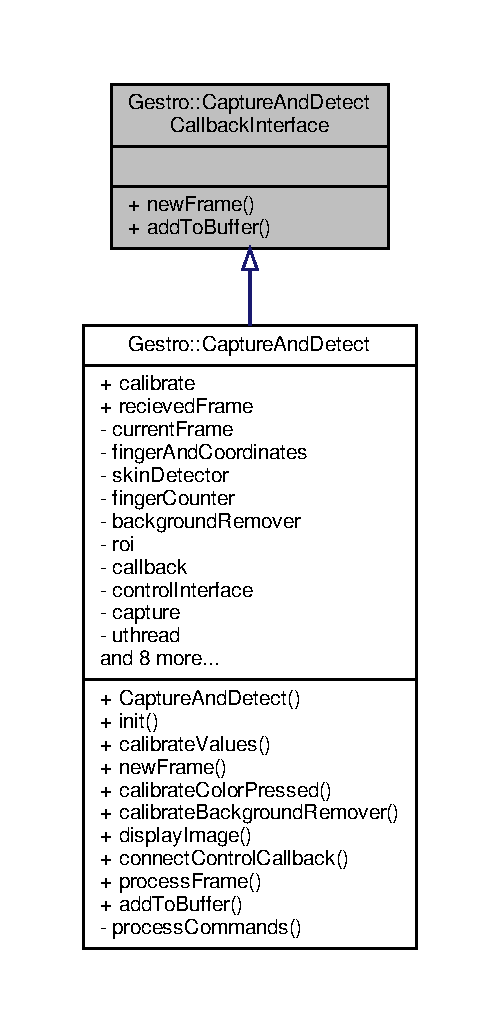
\includegraphics[width=240pt]{class_gestro_1_1_capture_and_detect_callback_interface__inherit__graph}
\end{center}
\end{figure}


Collaboration diagram for Gestro\+:\+:Capture\+And\+Detect\+Callback\+Interface\+:
\nopagebreak
\begin{figure}[H]
\begin{center}
\leavevmode
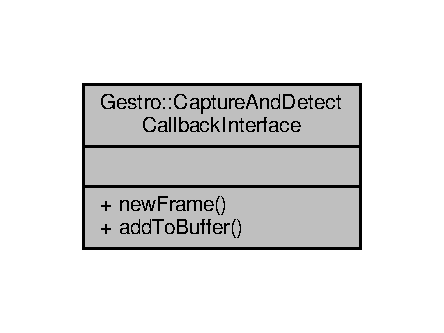
\includegraphics[width=213pt]{class_gestro_1_1_capture_and_detect_callback_interface__coll__graph}
\end{center}
\end{figure}
\subsection*{Public Member Functions}
\begin{DoxyCompactItemize}
\item 
virtual void \hyperlink{class_gestro_1_1_capture_and_detect_callback_interface_a9a42d0f1b3fd64cea607eeb4e6a46287}{new\+Frame} (Mat)=0
\begin{DoxyCompactList}\small\item\em virtual method to update new\+Frame \end{DoxyCompactList}\item 
virtual void \hyperlink{class_gestro_1_1_capture_and_detect_callback_interface_a8397891f6177ba6257e9cc978d9ddd52}{add\+To\+Buffer} (\hyperlink{class_gesture_detection_1_1_finger_and_coordinates}{Finger\+And\+Coordinates})=0
\begin{DoxyCompactList}\small\item\em virtual method to add data to buffer \end{DoxyCompactList}\end{DoxyCompactItemize}


\subsection{Detailed Description}
Callback interface for \hyperlink{class_gestro_1_1_capture_and_detect}{Capture\+And\+Detect}. 

Definition at line 12 of file Capture\+And\+Detect\+Callback\+Interface.\+h.



\subsection{Member Function Documentation}
\mbox{\Hypertarget{class_gestro_1_1_capture_and_detect_callback_interface_a8397891f6177ba6257e9cc978d9ddd52}\label{class_gestro_1_1_capture_and_detect_callback_interface_a8397891f6177ba6257e9cc978d9ddd52}} 
\index{Gestro\+::\+Capture\+And\+Detect\+Callback\+Interface@{Gestro\+::\+Capture\+And\+Detect\+Callback\+Interface}!add\+To\+Buffer@{add\+To\+Buffer}}
\index{add\+To\+Buffer@{add\+To\+Buffer}!Gestro\+::\+Capture\+And\+Detect\+Callback\+Interface@{Gestro\+::\+Capture\+And\+Detect\+Callback\+Interface}}
\subsubsection{\texorpdfstring{add\+To\+Buffer()}{addToBuffer()}}
{\footnotesize\ttfamily virtual void Gestro\+::\+Capture\+And\+Detect\+Callback\+Interface\+::add\+To\+Buffer (\begin{DoxyParamCaption}\item[{\hyperlink{class_gesture_detection_1_1_finger_and_coordinates}{Finger\+And\+Coordinates}}]{ }\end{DoxyParamCaption})\hspace{0.3cm}{\ttfamily [pure virtual]}}



virtual method to add data to buffer 



Implemented in \hyperlink{class_gestro_1_1_capture_and_detect_af376ab5418f7b235ee181d574da71fd6}{Gestro\+::\+Capture\+And\+Detect}.

\mbox{\Hypertarget{class_gestro_1_1_capture_and_detect_callback_interface_a9a42d0f1b3fd64cea607eeb4e6a46287}\label{class_gestro_1_1_capture_and_detect_callback_interface_a9a42d0f1b3fd64cea607eeb4e6a46287}} 
\index{Gestro\+::\+Capture\+And\+Detect\+Callback\+Interface@{Gestro\+::\+Capture\+And\+Detect\+Callback\+Interface}!new\+Frame@{new\+Frame}}
\index{new\+Frame@{new\+Frame}!Gestro\+::\+Capture\+And\+Detect\+Callback\+Interface@{Gestro\+::\+Capture\+And\+Detect\+Callback\+Interface}}
\subsubsection{\texorpdfstring{new\+Frame()}{newFrame()}}
{\footnotesize\ttfamily virtual void Gestro\+::\+Capture\+And\+Detect\+Callback\+Interface\+::new\+Frame (\begin{DoxyParamCaption}\item[{Mat}]{ }\end{DoxyParamCaption})\hspace{0.3cm}{\ttfamily [pure virtual]}}



virtual method to update new\+Frame 



Implemented in \hyperlink{class_gestro_1_1_capture_and_detect_a7f18d1c58b2ae4241766b36aa27385e9}{Gestro\+::\+Capture\+And\+Detect}.

Here is the caller graph for this function\+:
\nopagebreak
\begin{figure}[H]
\begin{center}
\leavevmode
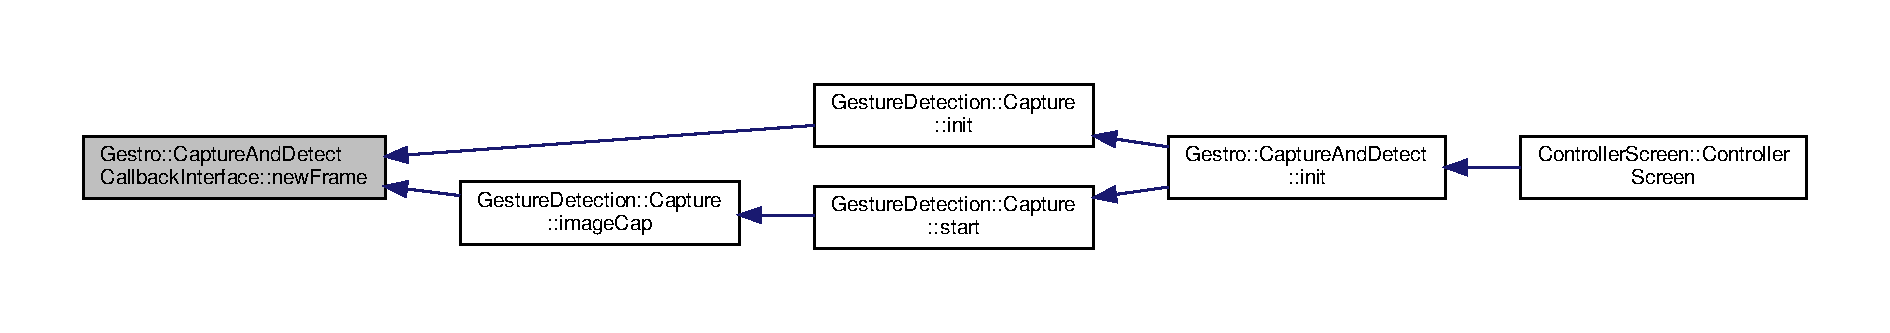
\includegraphics[width=350pt]{class_gestro_1_1_capture_and_detect_callback_interface_a9a42d0f1b3fd64cea607eeb4e6a46287_icgraph}
\end{center}
\end{figure}


The documentation for this class was generated from the following file\+:\begin{DoxyCompactItemize}
\item 
src/gesture\+\_\+detection/\hyperlink{_capture_and_detect_callback_interface_8h}{Capture\+And\+Detect\+Callback\+Interface.\+h}\end{DoxyCompactItemize}

\hypertarget{class_controller_screen}{}\section{Controller\+Screen Class Reference}
\label{class_controller_screen}\index{Controller\+Screen@{Controller\+Screen}}


It sets up the G\+UI, initializes Capture\+And\+Detect, and Display\+Control.  




{\ttfamily \#include $<$Controller\+Screen.\+h$>$}



Inheritance diagram for Controller\+Screen\+:
\nopagebreak
\begin{figure}[H]
\begin{center}
\leavevmode
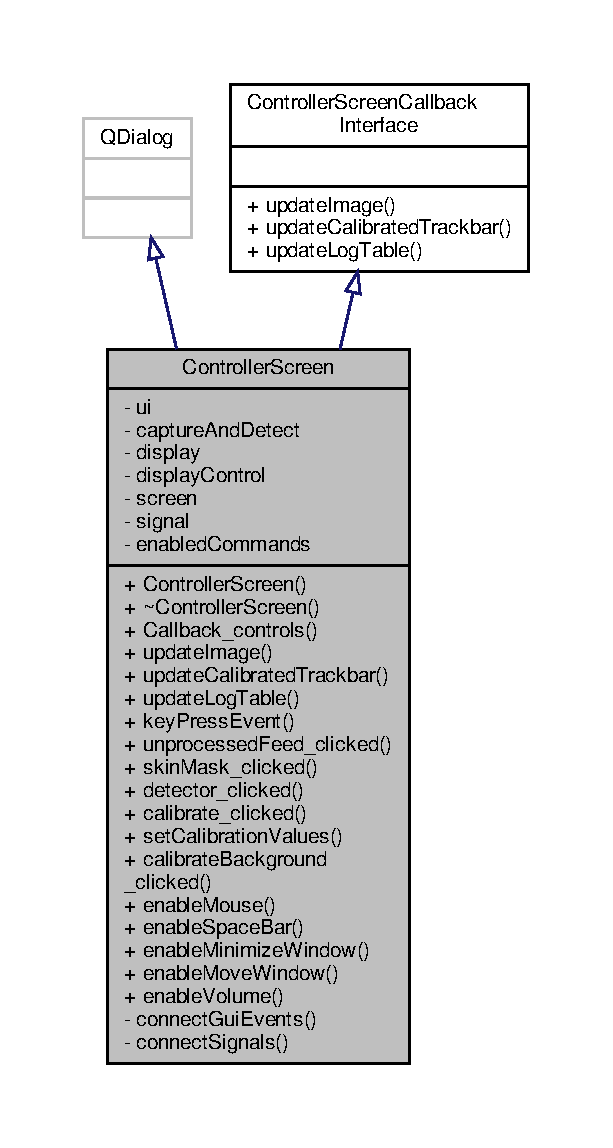
\includegraphics[height=550pt]{class_controller_screen__inherit__graph}
\end{center}
\end{figure}


Collaboration diagram for Controller\+Screen\+:
\nopagebreak
\begin{figure}[H]
\begin{center}
\leavevmode
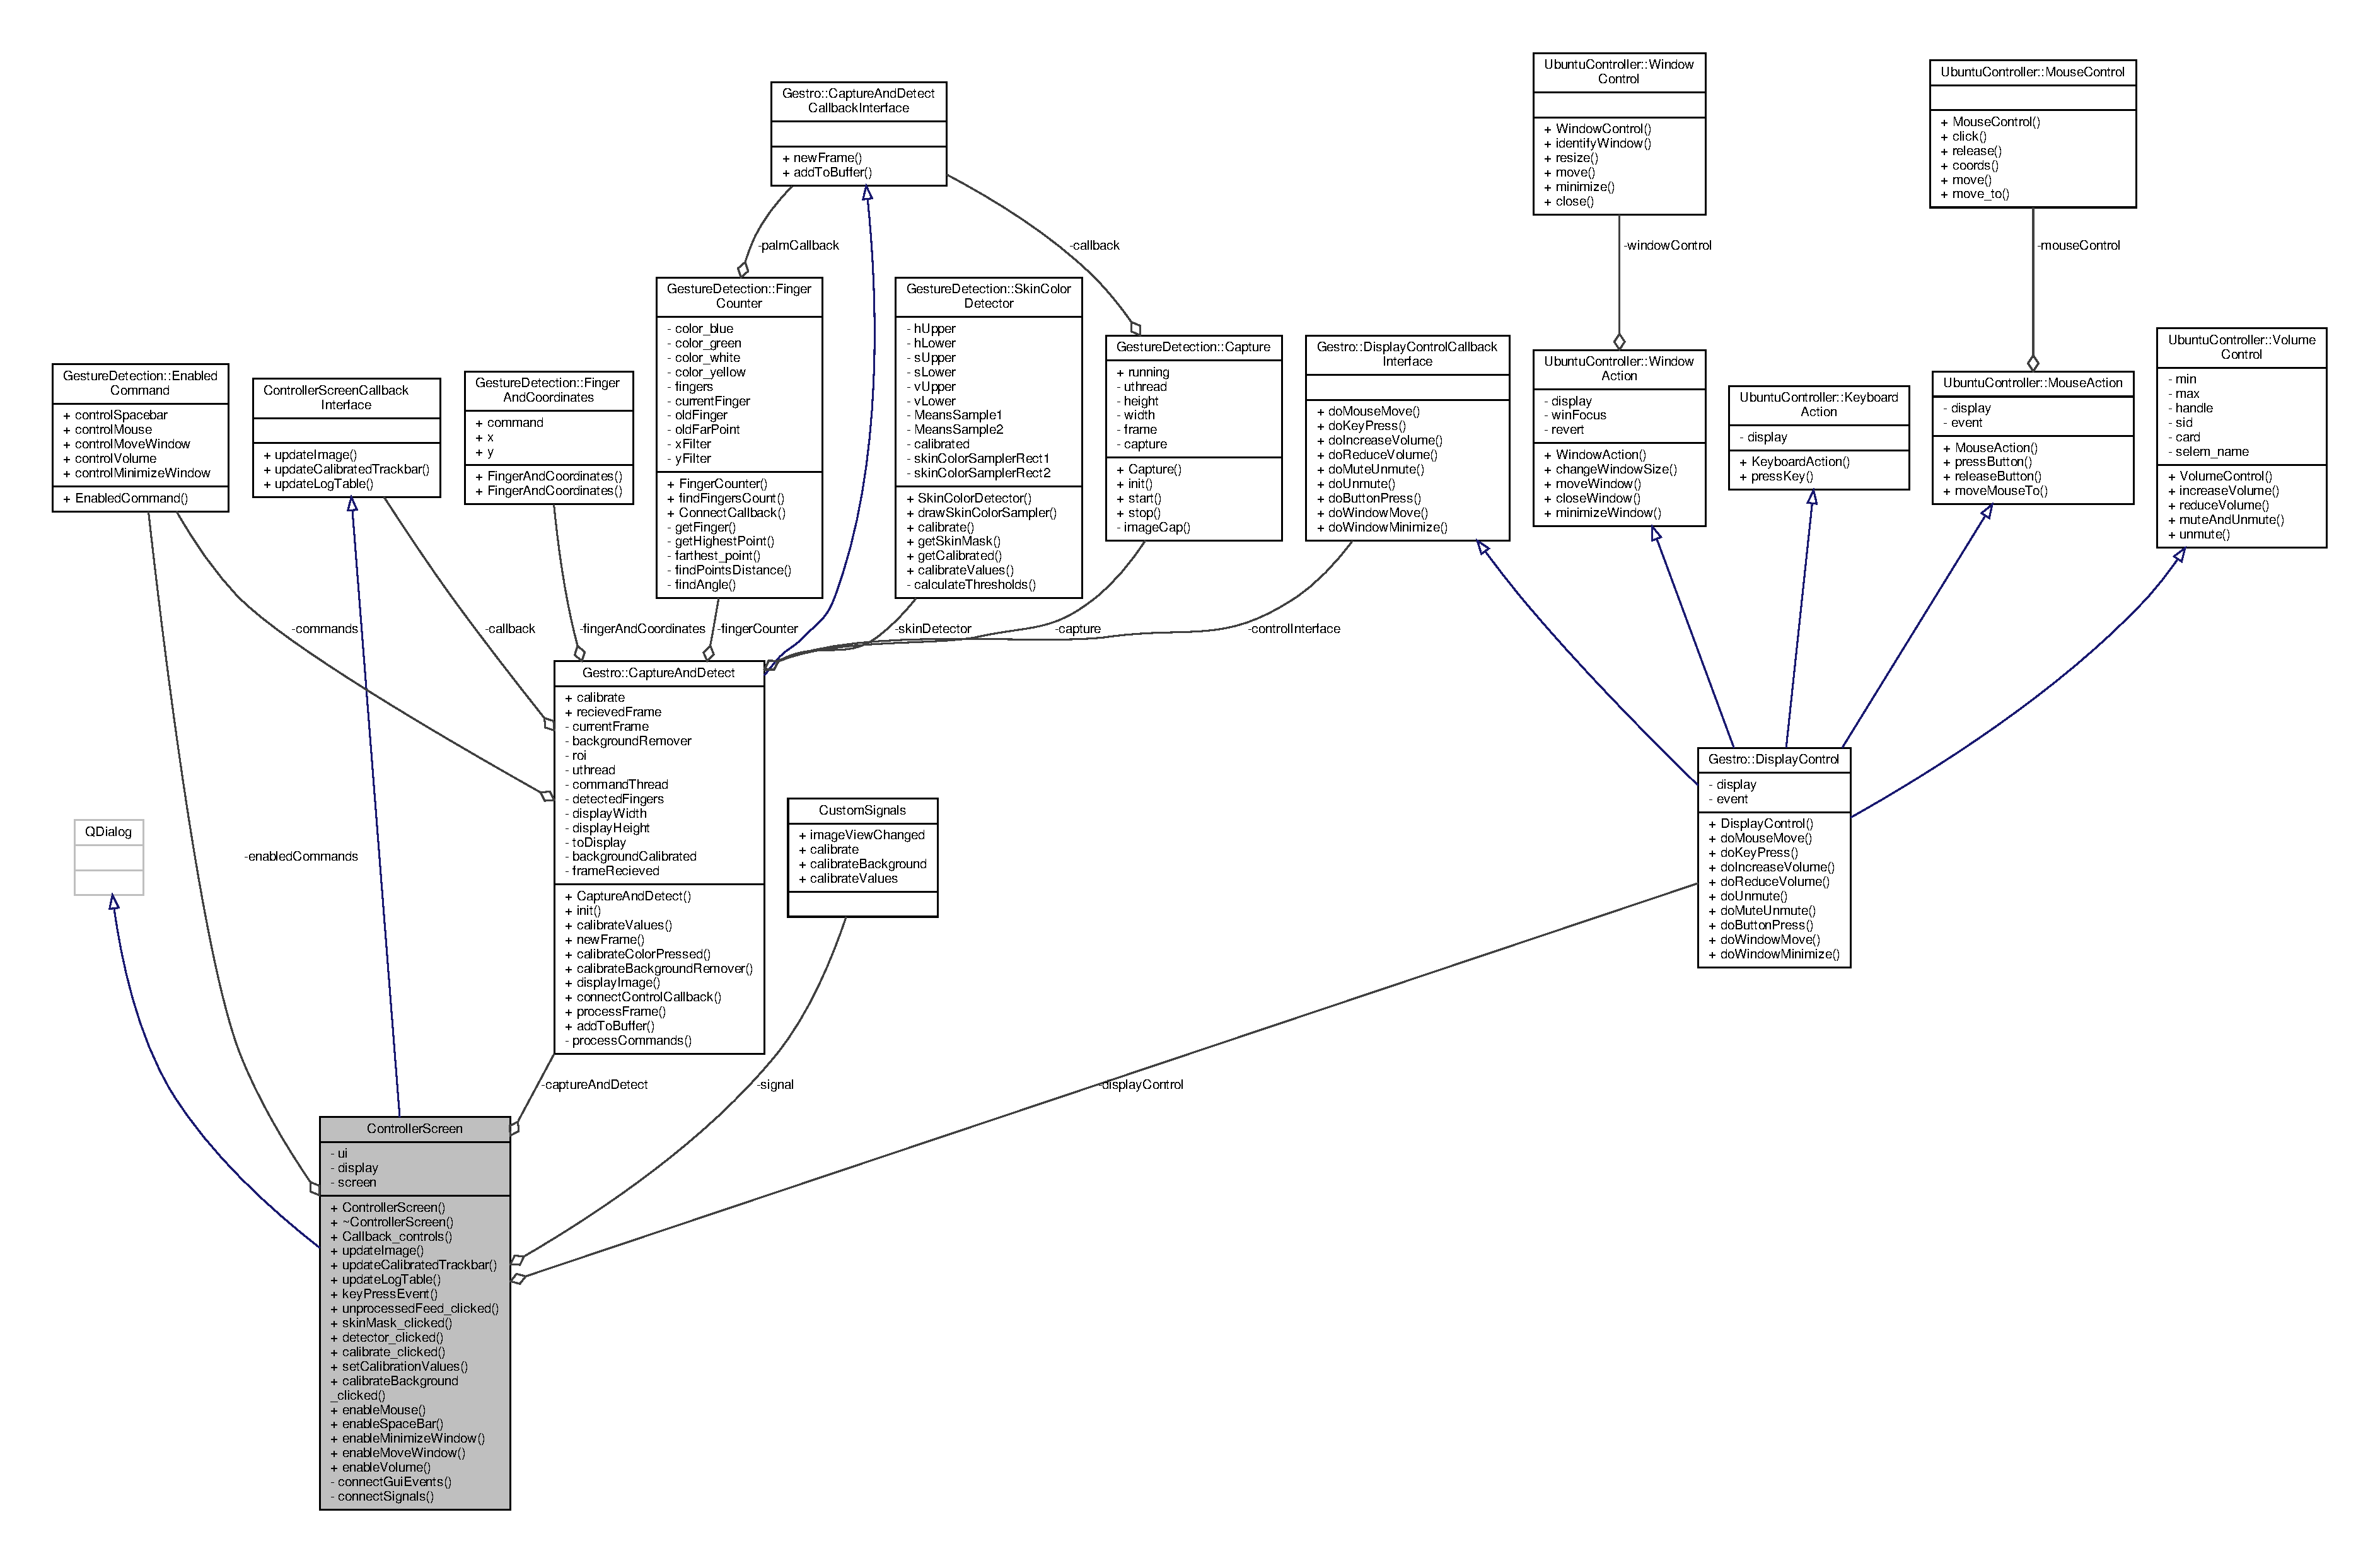
\includegraphics[width=350pt]{class_controller_screen__coll__graph}
\end{center}
\end{figure}
\subsection*{Public Slots}
\begin{DoxyCompactItemize}
\item 
void \hyperlink{class_controller_screen_aac8b2856372fa02c4f793cf9183dffed}{unprocessed\+Feed\+\_\+clicked} ()
\item 
void \hyperlink{class_controller_screen_a4d9db4a832f667aacb7d7532f752fd1b}{skin\+Mask\+\_\+clicked} ()
\item 
void \hyperlink{class_controller_screen_ac4f535408ffdfa10cbfa1a89d833f592}{detector\+\_\+clicked} ()
\item 
void \hyperlink{class_controller_screen_af7f51cf63bb9d2526b0025f35f1e7731}{calibrate\+\_\+clicked} ()
\item 
void \hyperlink{class_controller_screen_ae4d6a51231fb1f6f8809ce3d036592bd}{set\+Calibration\+Values} ()
\item 
void \hyperlink{class_controller_screen_a7a71b9bc26a3de704f8613f3f2a08fb7}{calibrate\+Background\+\_\+clicked} ()
\item 
void \hyperlink{class_controller_screen_a27681be09b97984576a895ad21343b65}{enable\+Mouse} ()
\item 
void \hyperlink{class_controller_screen_aa75c31cfb62427bba649b30e58130bfc}{enable\+Space\+Bar} ()
\item 
void \hyperlink{class_controller_screen_ad27b95368191153fa12d05091728b022}{enable\+Minimize\+Window} ()
\item 
void \hyperlink{class_controller_screen_a90e6dcfb4a0dfb2e845890bba3f208f5}{enable\+Move\+Window} ()
\item 
void \hyperlink{class_controller_screen_ae08e0ea89830d8018ff9086e4c4362a5}{enable\+Volume} ()
\end{DoxyCompactItemize}
\subsection*{Public Member Functions}
\begin{DoxyCompactItemize}
\item 
\hyperlink{class_controller_screen_aecef7737326dbb37945e6a9eac6dcede}{Controller\+Screen} (Q\+Widget $\ast$parent=0)
\item 
\hyperlink{class_controller_screen_a4871b73dbeec4679ba6bee692bfe71a9}{$\sim$\+Controller\+Screen} ()
\item 
void \hyperlink{class_controller_screen_a54062624a4a89d8bf392ab5fa66ac5ff}{Callback\+\_\+controls} (\hyperlink{class_gesture_detection_1_1_finger_and_coordinates}{Finger\+And\+Coordinates} finger)
\item 
void \hyperlink{class_controller_screen_acf75ddc9588011e360e2199cc37478ec}{update\+Image} (Mat) override
\item 
void \hyperlink{class_controller_screen_a700c8c1911e68861b86890a5429d2692}{update\+Calibrated\+Trackbar} (int, int, int, int) override
\item 
void \hyperlink{class_controller_screen_a039b816adc94fc7e7757520c10fd1d0b}{update\+Log\+Table} (String a, String b) override
\item 
void \hyperlink{class_controller_screen_afbb0033f9be00fce83d54f2a49b9ba89}{key\+Press\+Event} (Q\+Key\+Event $\ast$) override
\end{DoxyCompactItemize}
\subsection*{Private Member Functions}
\begin{DoxyCompactItemize}
\item 
void \hyperlink{class_controller_screen_acf89cc74ff8383884d11a067b3243d4a}{connect\+Gui\+Events} ()
\item 
void \hyperlink{class_controller_screen_af7c789ddca1dece0fb0585e84aeb5e81}{connect\+Signals} ()
\end{DoxyCompactItemize}
\subsection*{Private Attributes}
\begin{DoxyCompactItemize}
\item 
Ui\+::\+Controller\+Screen $\ast$ \hyperlink{class_controller_screen_a25a37166616a171730a89ddb69c120f3}{ui}
\begin{DoxyCompactList}\small\item\em A pointer to the ui class. \end{DoxyCompactList}\item 
\hyperlink{class_gestro_1_1_capture_and_detect}{Capture\+And\+Detect} \hyperlink{class_controller_screen_a672477c37c55499b69e28da611e7313d}{capture\+And\+Detect}
\begin{DoxyCompactList}\small\item\em Creating an instance of the Capture\+And\+Detect class. \end{DoxyCompactList}\item 
Display $\ast$ \hyperlink{class_controller_screen_a240495b9e446bc512d8a7498b3f45981}{display} = X\+Open\+Display(N\+U\+LL)
\begin{DoxyCompactList}\small\item\em Opening a connection to the X server. \end{DoxyCompactList}\item 
\hyperlink{class_gestro_1_1_display_control}{Display\+Control} \hyperlink{class_controller_screen_a261f7eb9894dbcfdbddad62ad125e330}{display\+Control} = \hyperlink{class_gestro_1_1_display_control}{Display\+Control}(\hyperlink{class_controller_screen_a240495b9e446bc512d8a7498b3f45981}{display})
\begin{DoxyCompactList}\small\item\em Creating an instance of the Display\+Control class. \end{DoxyCompactList}\item 
Screen $\ast$ \hyperlink{class_controller_screen_ae667566a3438ae194170858cd328053e}{screen} = Default\+Screen\+Of\+Display(\hyperlink{class_controller_screen_a240495b9e446bc512d8a7498b3f45981}{display})
\begin{DoxyCompactList}\small\item\em Getting the default screen of the display. \end{DoxyCompactList}\item 
\hyperlink{struct_custom_signals}{Custom\+Signals} \hyperlink{class_controller_screen_afe5953fdc933fcc35cf0ef841c83f18c}{signal}
\begin{DoxyCompactList}\small\item\em Creating an instance of the \hyperlink{struct_custom_signals}{Custom\+Signals} class. \end{DoxyCompactList}\item 
\hyperlink{class_gesture_detection_1_1_enabled_command}{Enabled\+Command} \hyperlink{class_controller_screen_a96533700d5a3a0593d9b9d24a724b16b}{enabled\+Commands}
\begin{DoxyCompactList}\small\item\em A class that is used to store the enabled commands. \end{DoxyCompactList}\end{DoxyCompactItemize}


\subsection{Detailed Description}
It sets up the G\+UI, initializes Capture\+And\+Detect, and Display\+Control. 

Connects the G\+UI events to the appropriate functions, and connects the signals to the appropriate slots


\begin{DoxyParams}{Parameters}
{\em parent} & The parent widget of the dialog. \\
\hline
\end{DoxyParams}


Definition at line 39 of file Controller\+Screen.\+h.



\subsection{Constructor \& Destructor Documentation}
\mbox{\Hypertarget{class_controller_screen_aecef7737326dbb37945e6a9eac6dcede}\label{class_controller_screen_aecef7737326dbb37945e6a9eac6dcede}} 
\index{Controller\+Screen@{Controller\+Screen}!Controller\+Screen@{Controller\+Screen}}
\index{Controller\+Screen@{Controller\+Screen}!Controller\+Screen@{Controller\+Screen}}
\subsubsection{\texorpdfstring{Controller\+Screen()}{ControllerScreen()}}
{\footnotesize\ttfamily Controller\+Screen\+::\+Controller\+Screen (\begin{DoxyParamCaption}\item[{Q\+Widget $\ast$}]{parent = {\ttfamily 0} }\end{DoxyParamCaption})\hspace{0.3cm}{\ttfamily [explicit]}}

Construtor 
\begin{DoxyParams}{Parameters}
{\em parent} & \\
\hline
\end{DoxyParams}


Definition at line 4 of file Controller\+Screen.\+cpp.

Here is the call graph for this function\+:
\nopagebreak
\begin{figure}[H]
\begin{center}
\leavevmode
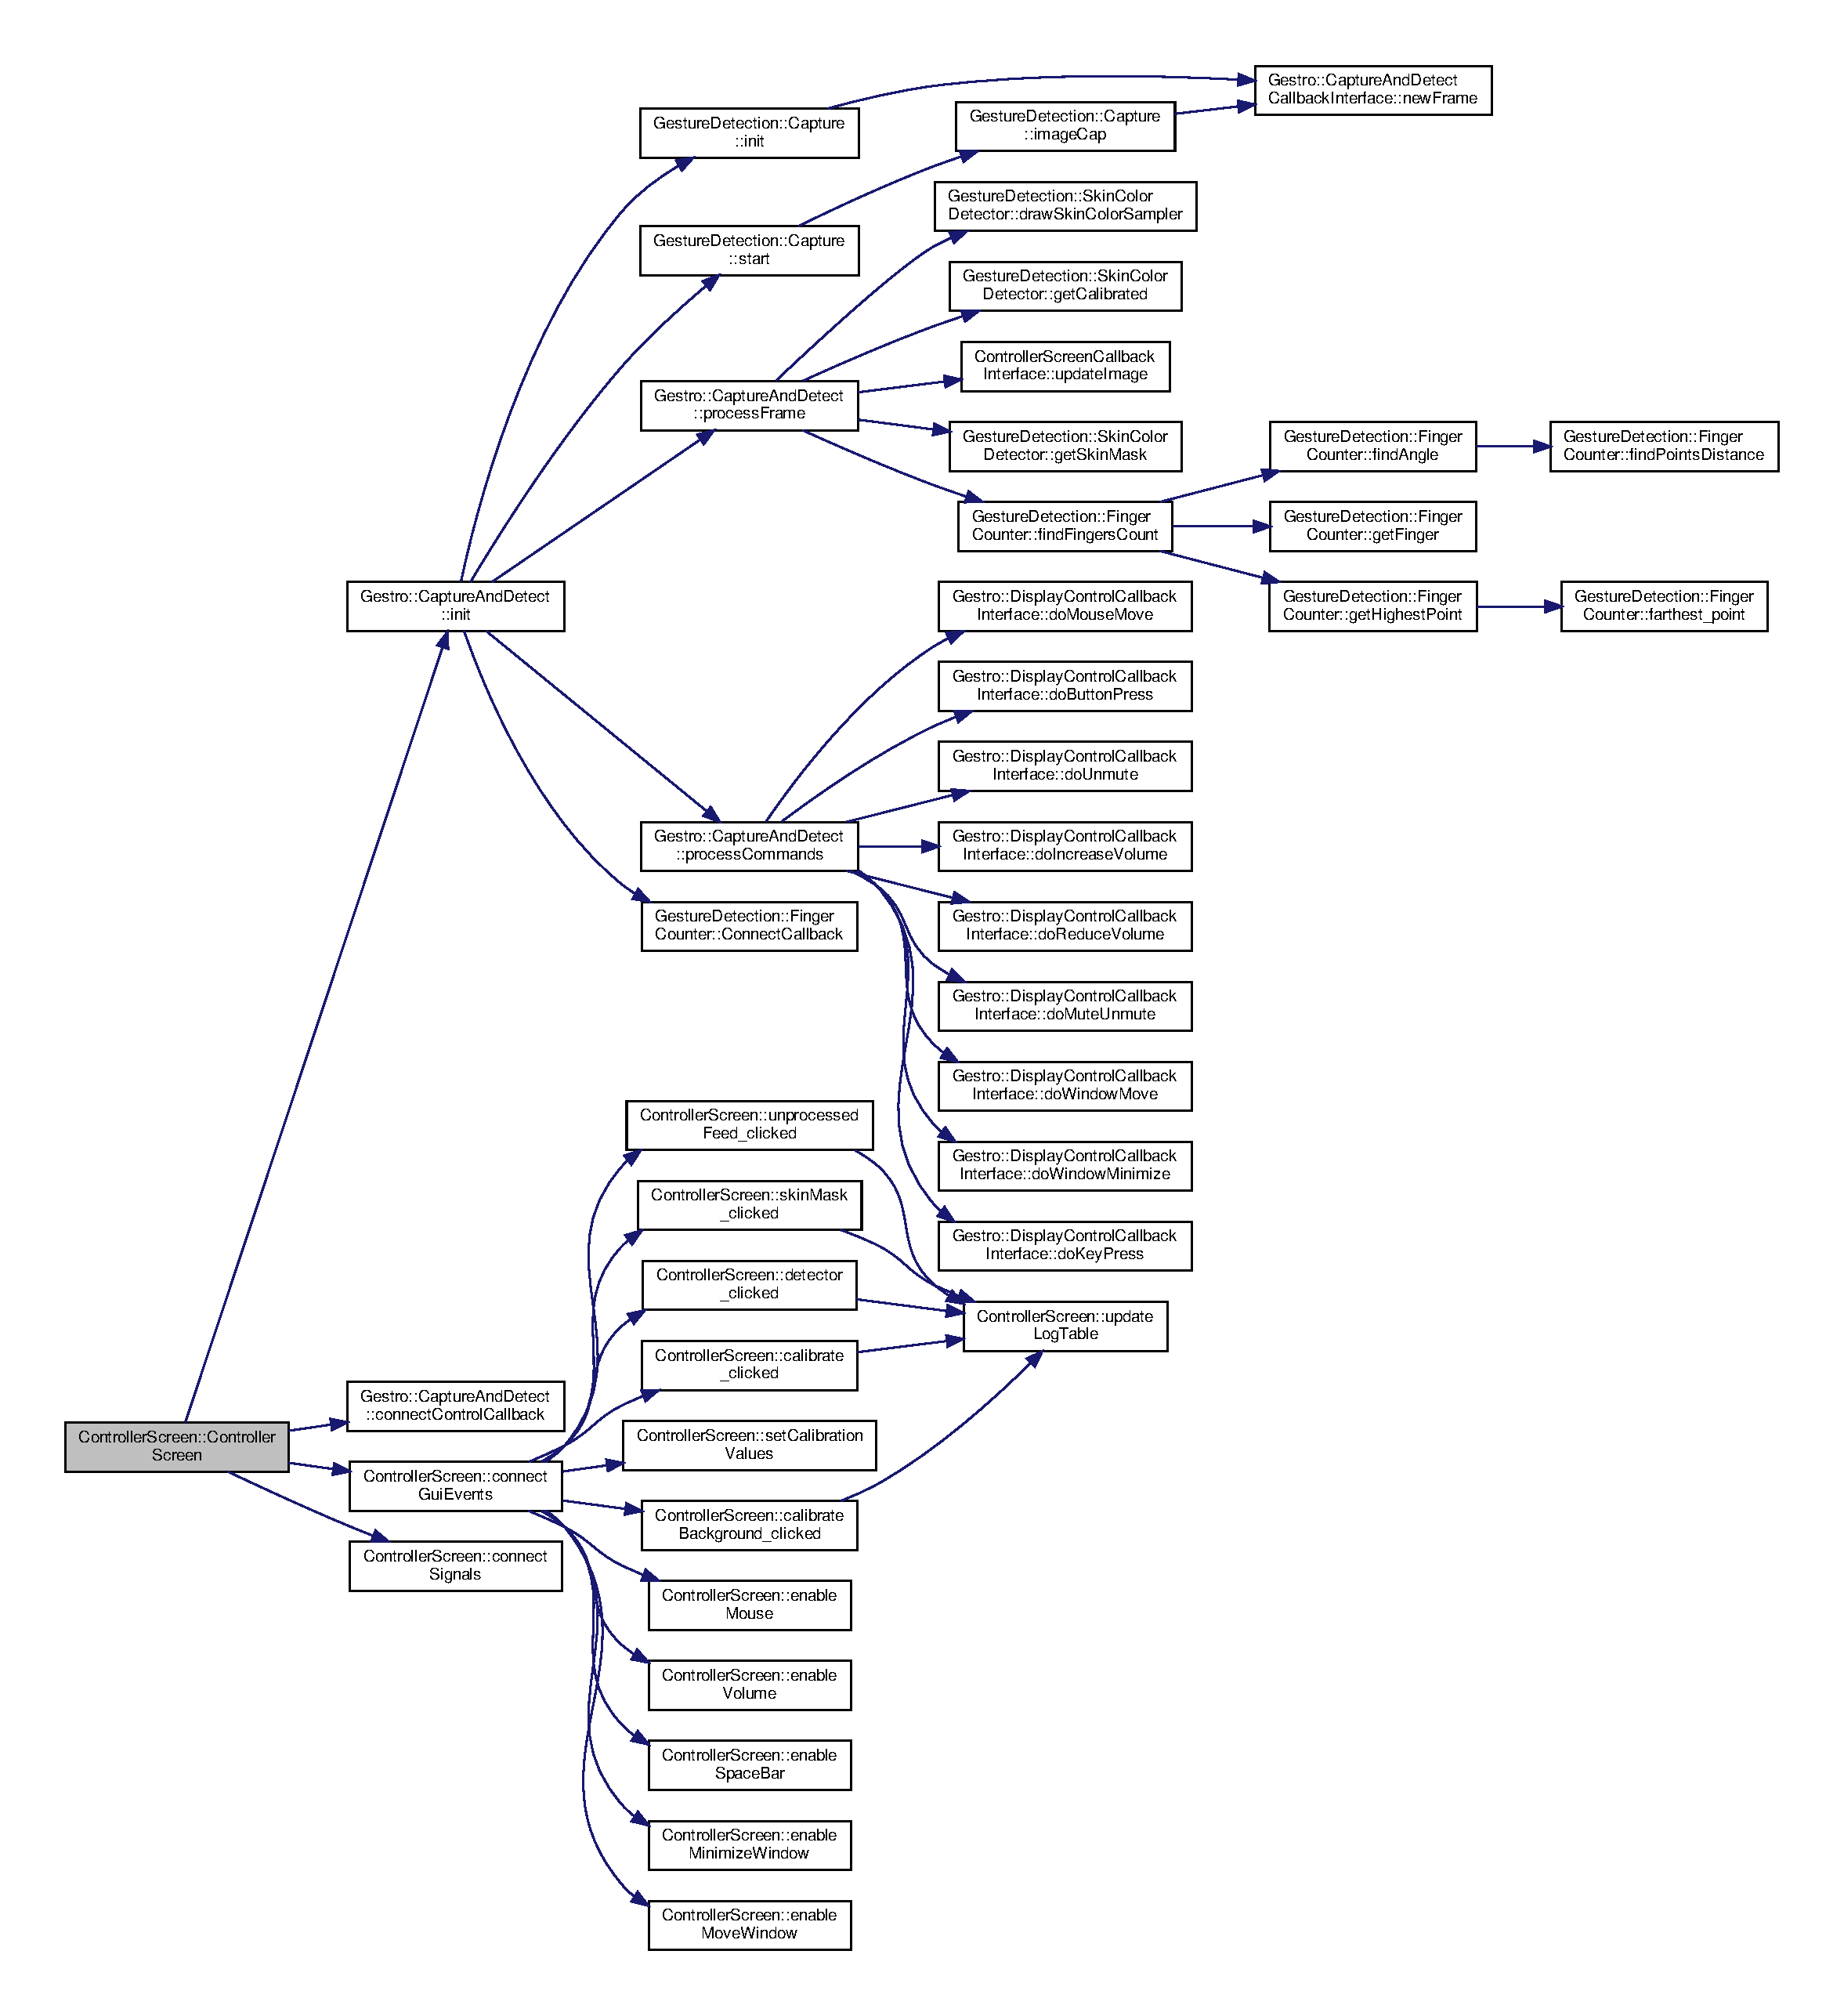
\includegraphics[width=350pt]{class_controller_screen_aecef7737326dbb37945e6a9eac6dcede_cgraph}
\end{center}
\end{figure}
\mbox{\Hypertarget{class_controller_screen_a4871b73dbeec4679ba6bee692bfe71a9}\label{class_controller_screen_a4871b73dbeec4679ba6bee692bfe71a9}} 
\index{Controller\+Screen@{Controller\+Screen}!````~Controller\+Screen@{$\sim$\+Controller\+Screen}}
\index{````~Controller\+Screen@{$\sim$\+Controller\+Screen}!Controller\+Screen@{Controller\+Screen}}
\subsubsection{\texorpdfstring{$\sim$\+Controller\+Screen()}{~ControllerScreen()}}
{\footnotesize\ttfamily Controller\+Screen\+::$\sim$\+Controller\+Screen (\begin{DoxyParamCaption}{ }\end{DoxyParamCaption})}

The destructor for the \hyperlink{class_controller_screen}{Controller\+Screen} class. 

Definition at line 52 of file Controller\+Screen.\+cpp.



\subsection{Member Function Documentation}
\mbox{\Hypertarget{class_controller_screen_af7f51cf63bb9d2526b0025f35f1e7731}\label{class_controller_screen_af7f51cf63bb9d2526b0025f35f1e7731}} 
\index{Controller\+Screen@{Controller\+Screen}!calibrate\+\_\+clicked@{calibrate\+\_\+clicked}}
\index{calibrate\+\_\+clicked@{calibrate\+\_\+clicked}!Controller\+Screen@{Controller\+Screen}}
\subsubsection{\texorpdfstring{calibrate\+\_\+clicked}{calibrate\_clicked}}
{\footnotesize\ttfamily void Controller\+Screen\+::calibrate\+\_\+clicked (\begin{DoxyParamCaption}{ }\end{DoxyParamCaption})\hspace{0.3cm}{\ttfamily [slot]}}

When the calibrate button is clicked, the skin mask and detector buttons are enabled, the calibrate button is disabled, the calibrate signal is emitted, the image view is changed to the skin mask, and the log table is updated 

Definition at line 79 of file Controller\+Screen.\+cpp.

Here is the call graph for this function\+:
\nopagebreak
\begin{figure}[H]
\begin{center}
\leavevmode
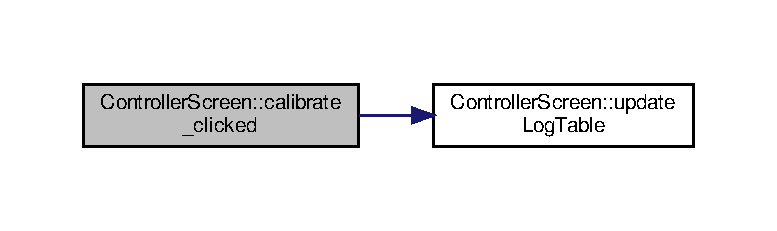
\includegraphics[width=350pt]{class_controller_screen_af7f51cf63bb9d2526b0025f35f1e7731_cgraph}
\end{center}
\end{figure}
Here is the caller graph for this function\+:
\nopagebreak
\begin{figure}[H]
\begin{center}
\leavevmode
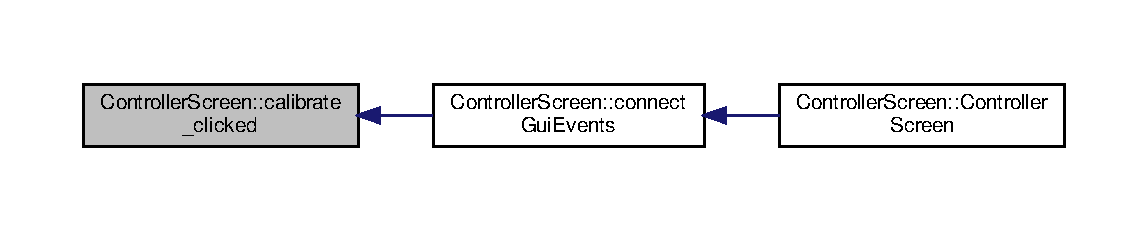
\includegraphics[width=350pt]{class_controller_screen_af7f51cf63bb9d2526b0025f35f1e7731_icgraph}
\end{center}
\end{figure}
\mbox{\Hypertarget{class_controller_screen_a7a71b9bc26a3de704f8613f3f2a08fb7}\label{class_controller_screen_a7a71b9bc26a3de704f8613f3f2a08fb7}} 
\index{Controller\+Screen@{Controller\+Screen}!calibrate\+Background\+\_\+clicked@{calibrate\+Background\+\_\+clicked}}
\index{calibrate\+Background\+\_\+clicked@{calibrate\+Background\+\_\+clicked}!Controller\+Screen@{Controller\+Screen}}
\subsubsection{\texorpdfstring{calibrate\+Background\+\_\+clicked}{calibrateBackground\_clicked}}
{\footnotesize\ttfamily void Controller\+Screen\+::calibrate\+Background\+\_\+clicked (\begin{DoxyParamCaption}{ }\end{DoxyParamCaption})\hspace{0.3cm}{\ttfamily [slot]}}

It calls the calibrate\+Background() function in the Signal class, and then updates the log table with a message 

Definition at line 89 of file Controller\+Screen.\+cpp.

Here is the call graph for this function\+:
\nopagebreak
\begin{figure}[H]
\begin{center}
\leavevmode
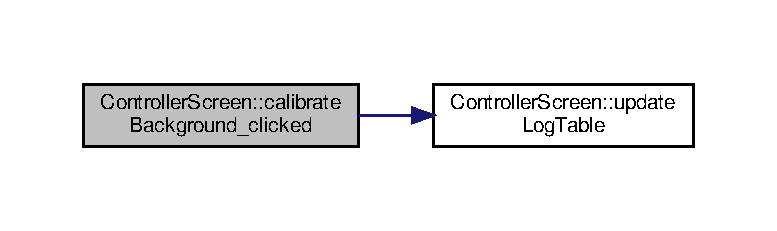
\includegraphics[width=350pt]{class_controller_screen_a7a71b9bc26a3de704f8613f3f2a08fb7_cgraph}
\end{center}
\end{figure}
Here is the caller graph for this function\+:
\nopagebreak
\begin{figure}[H]
\begin{center}
\leavevmode
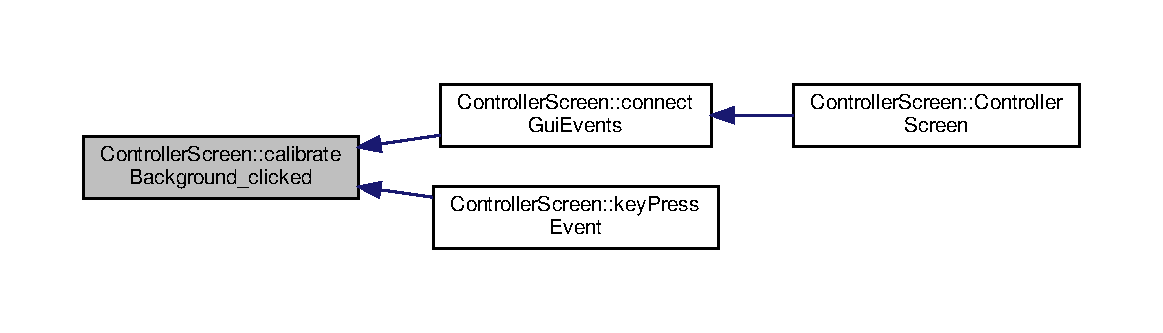
\includegraphics[width=350pt]{class_controller_screen_a7a71b9bc26a3de704f8613f3f2a08fb7_icgraph}
\end{center}
\end{figure}
\mbox{\Hypertarget{class_controller_screen_a54062624a4a89d8bf392ab5fa66ac5ff}\label{class_controller_screen_a54062624a4a89d8bf392ab5fa66ac5ff}} 
\index{Controller\+Screen@{Controller\+Screen}!Callback\+\_\+controls@{Callback\+\_\+controls}}
\index{Callback\+\_\+controls@{Callback\+\_\+controls}!Controller\+Screen@{Controller\+Screen}}
\subsubsection{\texorpdfstring{Callback\+\_\+controls()}{Callback\_controls()}}
{\footnotesize\ttfamily void Controller\+Screen\+::\+Callback\+\_\+controls (\begin{DoxyParamCaption}\item[{\hyperlink{class_gesture_detection_1_1_finger_and_coordinates}{Finger\+And\+Coordinates}}]{finger }\end{DoxyParamCaption})}

\mbox{\Hypertarget{class_controller_screen_acf89cc74ff8383884d11a067b3243d4a}\label{class_controller_screen_acf89cc74ff8383884d11a067b3243d4a}} 
\index{Controller\+Screen@{Controller\+Screen}!connect\+Gui\+Events@{connect\+Gui\+Events}}
\index{connect\+Gui\+Events@{connect\+Gui\+Events}!Controller\+Screen@{Controller\+Screen}}
\subsubsection{\texorpdfstring{connect\+Gui\+Events()}{connectGuiEvents()}}
{\footnotesize\ttfamily void Controller\+Screen\+::connect\+Gui\+Events (\begin{DoxyParamCaption}{ }\end{DoxyParamCaption})\hspace{0.3cm}{\ttfamily [private]}}

It connects the G\+UI elements to the appropriate slots 

Definition at line 34 of file Controller\+Screen.\+cpp.

Here is the call graph for this function\+:
\nopagebreak
\begin{figure}[H]
\begin{center}
\leavevmode
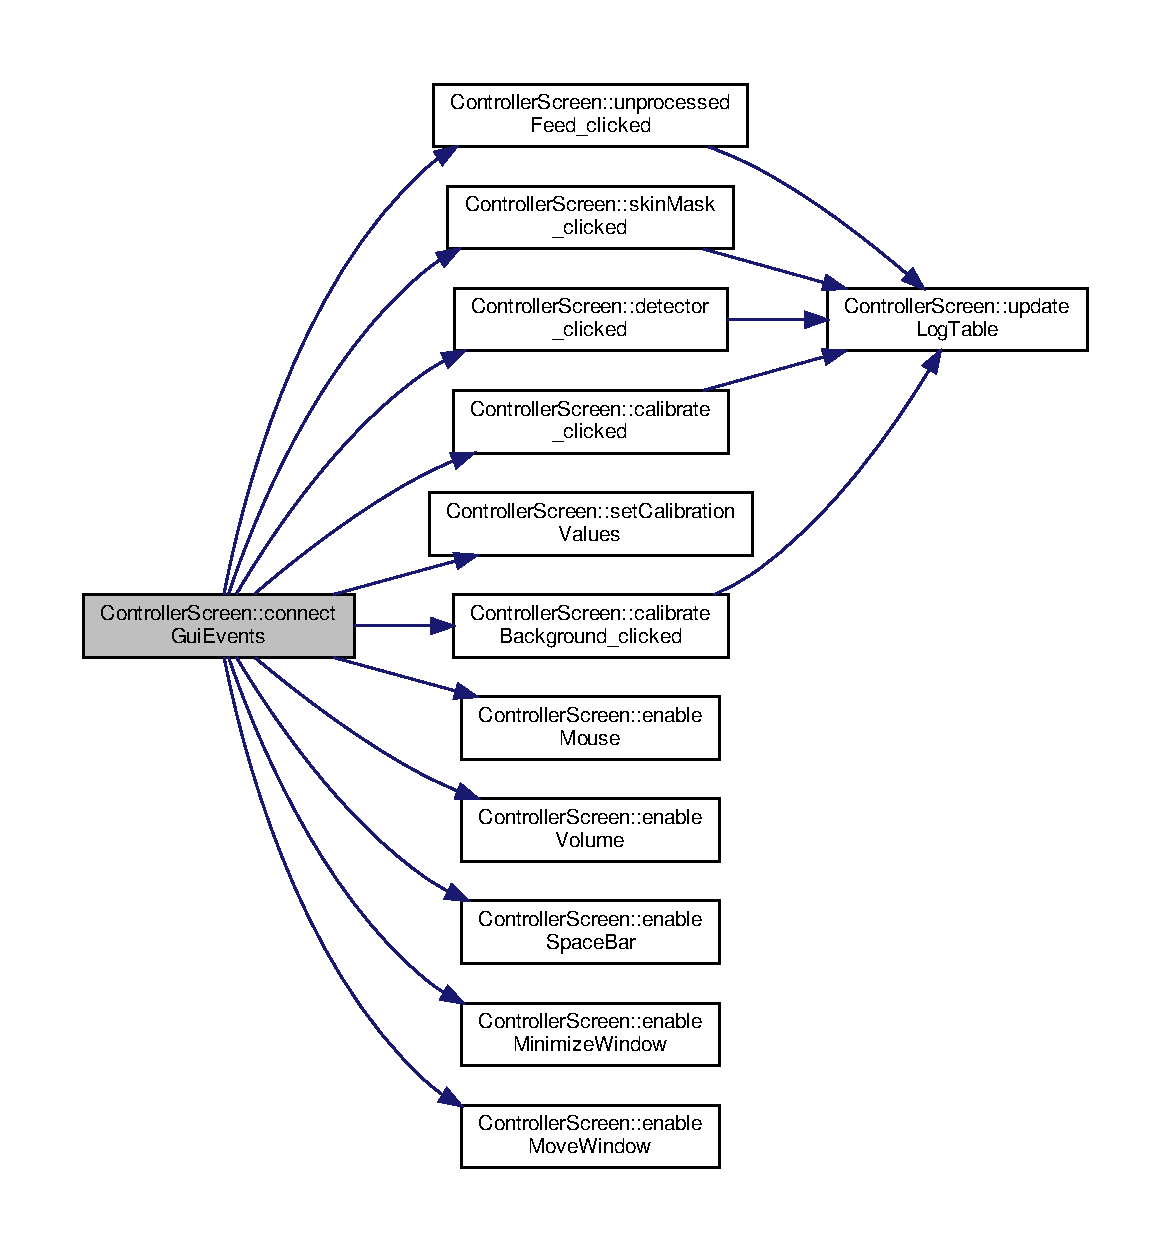
\includegraphics[width=350pt]{class_controller_screen_acf89cc74ff8383884d11a067b3243d4a_cgraph}
\end{center}
\end{figure}
Here is the caller graph for this function\+:
\nopagebreak
\begin{figure}[H]
\begin{center}
\leavevmode
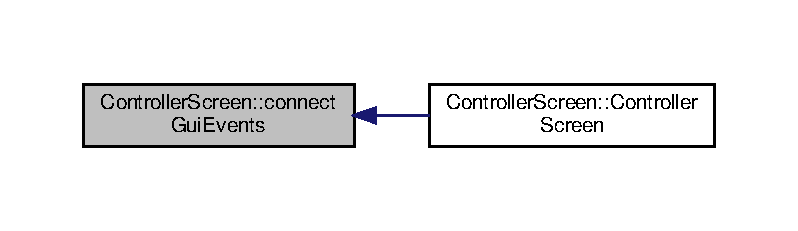
\includegraphics[width=350pt]{class_controller_screen_acf89cc74ff8383884d11a067b3243d4a_icgraph}
\end{center}
\end{figure}
\mbox{\Hypertarget{class_controller_screen_af7c789ddca1dece0fb0585e84aeb5e81}\label{class_controller_screen_af7c789ddca1dece0fb0585e84aeb5e81}} 
\index{Controller\+Screen@{Controller\+Screen}!connect\+Signals@{connect\+Signals}}
\index{connect\+Signals@{connect\+Signals}!Controller\+Screen@{Controller\+Screen}}
\subsubsection{\texorpdfstring{connect\+Signals()}{connectSignals()}}
{\footnotesize\ttfamily void Controller\+Screen\+::connect\+Signals (\begin{DoxyParamCaption}{ }\end{DoxyParamCaption})\hspace{0.3cm}{\ttfamily [private]}}

It connects the signals from the controller to the slots in the capture\+And\+Detect class 

Definition at line 26 of file Controller\+Screen.\+cpp.

Here is the caller graph for this function\+:
\nopagebreak
\begin{figure}[H]
\begin{center}
\leavevmode
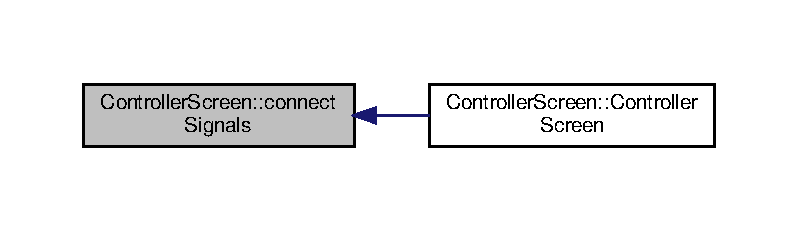
\includegraphics[width=350pt]{class_controller_screen_af7c789ddca1dece0fb0585e84aeb5e81_icgraph}
\end{center}
\end{figure}
\mbox{\Hypertarget{class_controller_screen_ac4f535408ffdfa10cbfa1a89d833f592}\label{class_controller_screen_ac4f535408ffdfa10cbfa1a89d833f592}} 
\index{Controller\+Screen@{Controller\+Screen}!detector\+\_\+clicked@{detector\+\_\+clicked}}
\index{detector\+\_\+clicked@{detector\+\_\+clicked}!Controller\+Screen@{Controller\+Screen}}
\subsubsection{\texorpdfstring{detector\+\_\+clicked}{detector\_clicked}}
{\footnotesize\ttfamily void Controller\+Screen\+::detector\+\_\+clicked (\begin{DoxyParamCaption}{ }\end{DoxyParamCaption})\hspace{0.3cm}{\ttfamily [slot]}}

It changes the image view to the finger counter 

Definition at line 72 of file Controller\+Screen.\+cpp.

Here is the call graph for this function\+:
\nopagebreak
\begin{figure}[H]
\begin{center}
\leavevmode
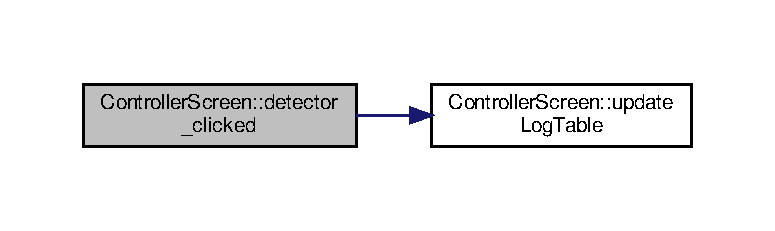
\includegraphics[width=350pt]{class_controller_screen_ac4f535408ffdfa10cbfa1a89d833f592_cgraph}
\end{center}
\end{figure}
Here is the caller graph for this function\+:
\nopagebreak
\begin{figure}[H]
\begin{center}
\leavevmode
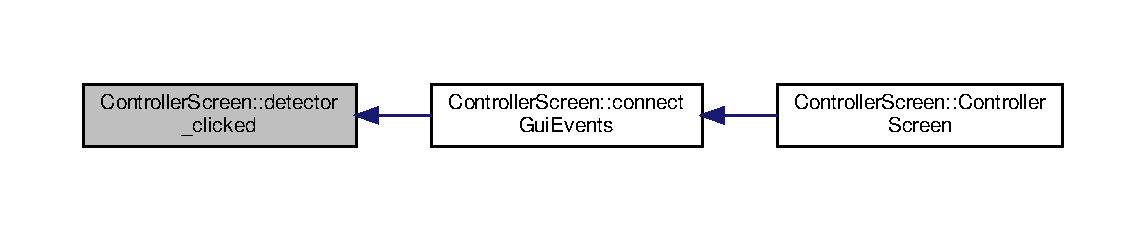
\includegraphics[width=350pt]{class_controller_screen_ac4f535408ffdfa10cbfa1a89d833f592_icgraph}
\end{center}
\end{figure}
\mbox{\Hypertarget{class_controller_screen_ad27b95368191153fa12d05091728b022}\label{class_controller_screen_ad27b95368191153fa12d05091728b022}} 
\index{Controller\+Screen@{Controller\+Screen}!enable\+Minimize\+Window@{enable\+Minimize\+Window}}
\index{enable\+Minimize\+Window@{enable\+Minimize\+Window}!Controller\+Screen@{Controller\+Screen}}
\subsubsection{\texorpdfstring{enable\+Minimize\+Window}{enableMinimizeWindow}}
{\footnotesize\ttfamily void Controller\+Screen\+::enable\+Minimize\+Window (\begin{DoxyParamCaption}{ }\end{DoxyParamCaption})\hspace{0.3cm}{\ttfamily [slot]}}

If the checkbox is checked, then the command is enabled 

Definition at line 148 of file Controller\+Screen.\+cpp.

Here is the caller graph for this function\+:
\nopagebreak
\begin{figure}[H]
\begin{center}
\leavevmode
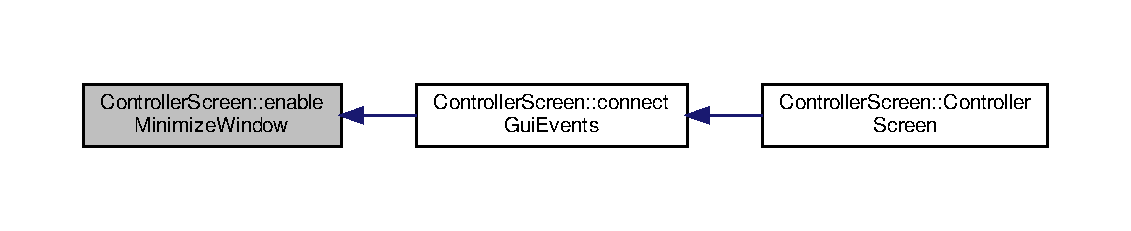
\includegraphics[width=350pt]{class_controller_screen_ad27b95368191153fa12d05091728b022_icgraph}
\end{center}
\end{figure}
\mbox{\Hypertarget{class_controller_screen_a27681be09b97984576a895ad21343b65}\label{class_controller_screen_a27681be09b97984576a895ad21343b65}} 
\index{Controller\+Screen@{Controller\+Screen}!enable\+Mouse@{enable\+Mouse}}
\index{enable\+Mouse@{enable\+Mouse}!Controller\+Screen@{Controller\+Screen}}
\subsubsection{\texorpdfstring{enable\+Mouse}{enableMouse}}
{\footnotesize\ttfamily void Controller\+Screen\+::enable\+Mouse (\begin{DoxyParamCaption}{ }\end{DoxyParamCaption})\hspace{0.3cm}{\ttfamily [slot]}}

If the checkbox is checked, then the control\+Mouse variable is set to true, otherwise it is set to false 

Definition at line 132 of file Controller\+Screen.\+cpp.

Here is the caller graph for this function\+:
\nopagebreak
\begin{figure}[H]
\begin{center}
\leavevmode
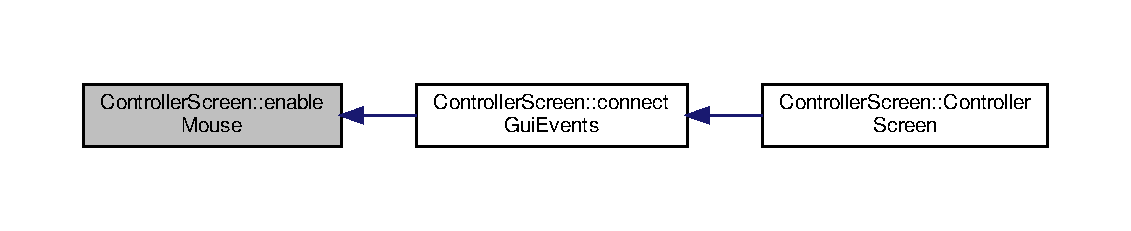
\includegraphics[width=350pt]{class_controller_screen_a27681be09b97984576a895ad21343b65_icgraph}
\end{center}
\end{figure}
\mbox{\Hypertarget{class_controller_screen_a90e6dcfb4a0dfb2e845890bba3f208f5}\label{class_controller_screen_a90e6dcfb4a0dfb2e845890bba3f208f5}} 
\index{Controller\+Screen@{Controller\+Screen}!enable\+Move\+Window@{enable\+Move\+Window}}
\index{enable\+Move\+Window@{enable\+Move\+Window}!Controller\+Screen@{Controller\+Screen}}
\subsubsection{\texorpdfstring{enable\+Move\+Window}{enableMoveWindow}}
{\footnotesize\ttfamily void Controller\+Screen\+::enable\+Move\+Window (\begin{DoxyParamCaption}{ }\end{DoxyParamCaption})\hspace{0.3cm}{\ttfamily [slot]}}

If the checkbox is checked, then the control\+Move\+Window variable is set to true, otherwise it is set to false 

Definition at line 156 of file Controller\+Screen.\+cpp.

Here is the caller graph for this function\+:
\nopagebreak
\begin{figure}[H]
\begin{center}
\leavevmode
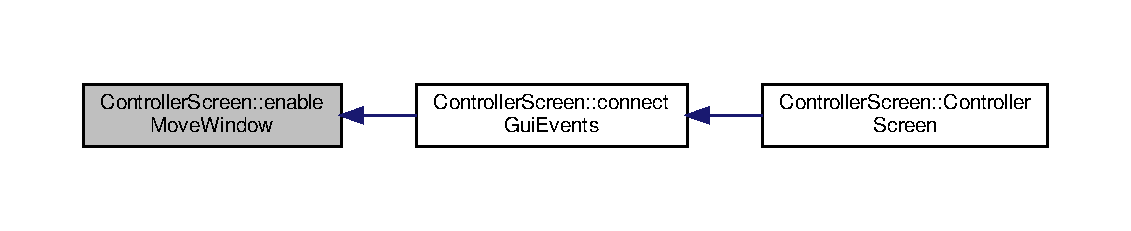
\includegraphics[width=350pt]{class_controller_screen_a90e6dcfb4a0dfb2e845890bba3f208f5_icgraph}
\end{center}
\end{figure}
\mbox{\Hypertarget{class_controller_screen_aa75c31cfb62427bba649b30e58130bfc}\label{class_controller_screen_aa75c31cfb62427bba649b30e58130bfc}} 
\index{Controller\+Screen@{Controller\+Screen}!enable\+Space\+Bar@{enable\+Space\+Bar}}
\index{enable\+Space\+Bar@{enable\+Space\+Bar}!Controller\+Screen@{Controller\+Screen}}
\subsubsection{\texorpdfstring{enable\+Space\+Bar}{enableSpaceBar}}
{\footnotesize\ttfamily void Controller\+Screen\+::enable\+Space\+Bar (\begin{DoxyParamCaption}{ }\end{DoxyParamCaption})\hspace{0.3cm}{\ttfamily [slot]}}

If the checkbox is checked, then the control\+Spacebar variable is set to true, otherwise it is set to false 

Definition at line 140 of file Controller\+Screen.\+cpp.

Here is the caller graph for this function\+:
\nopagebreak
\begin{figure}[H]
\begin{center}
\leavevmode
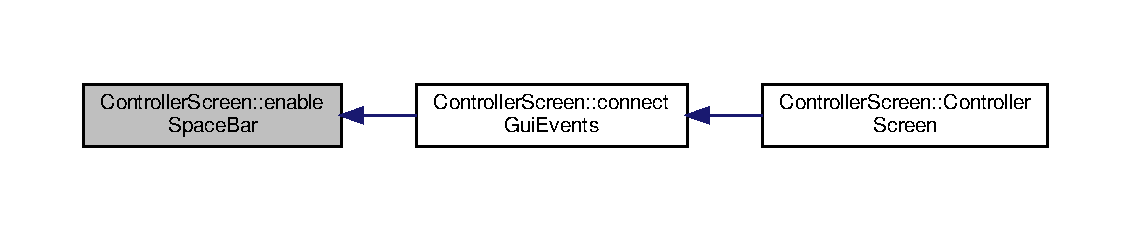
\includegraphics[width=350pt]{class_controller_screen_aa75c31cfb62427bba649b30e58130bfc_icgraph}
\end{center}
\end{figure}
\mbox{\Hypertarget{class_controller_screen_ae08e0ea89830d8018ff9086e4c4362a5}\label{class_controller_screen_ae08e0ea89830d8018ff9086e4c4362a5}} 
\index{Controller\+Screen@{Controller\+Screen}!enable\+Volume@{enable\+Volume}}
\index{enable\+Volume@{enable\+Volume}!Controller\+Screen@{Controller\+Screen}}
\subsubsection{\texorpdfstring{enable\+Volume}{enableVolume}}
{\footnotesize\ttfamily void Controller\+Screen\+::enable\+Volume (\begin{DoxyParamCaption}{ }\end{DoxyParamCaption})\hspace{0.3cm}{\ttfamily [slot]}}

If the checkbox is checked, then the control\+Volume variable is set to true, otherwise it is set to false 

Definition at line 165 of file Controller\+Screen.\+cpp.

Here is the caller graph for this function\+:
\nopagebreak
\begin{figure}[H]
\begin{center}
\leavevmode
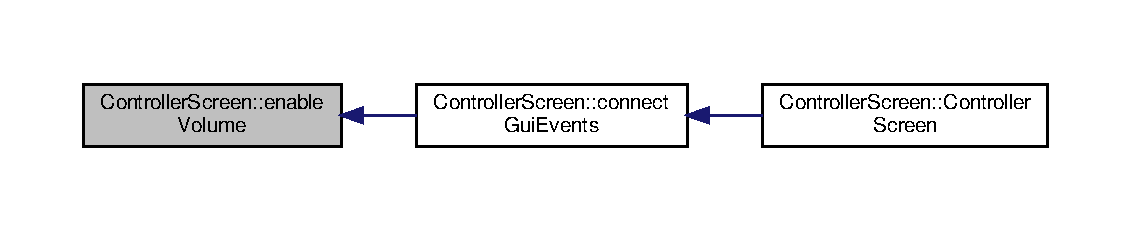
\includegraphics[width=350pt]{class_controller_screen_ae08e0ea89830d8018ff9086e4c4362a5_icgraph}
\end{center}
\end{figure}
\mbox{\Hypertarget{class_controller_screen_afbb0033f9be00fce83d54f2a49b9ba89}\label{class_controller_screen_afbb0033f9be00fce83d54f2a49b9ba89}} 
\index{Controller\+Screen@{Controller\+Screen}!key\+Press\+Event@{key\+Press\+Event}}
\index{key\+Press\+Event@{key\+Press\+Event}!Controller\+Screen@{Controller\+Screen}}
\subsubsection{\texorpdfstring{key\+Press\+Event()}{keyPressEvent()}}
{\footnotesize\ttfamily void Controller\+Screen\+::key\+Press\+Event (\begin{DoxyParamCaption}\item[{Q\+Key\+Event $\ast$}]{keypress }\end{DoxyParamCaption})\hspace{0.3cm}{\ttfamily [override]}}

If the user presses the \char`\"{}\+B\char`\"{} key, then the \hyperlink{class_controller_screen_a7a71b9bc26a3de704f8613f3f2a08fb7}{calibrate\+Background\+\_\+clicked()} function is called


\begin{DoxyParams}{Parameters}
{\em keypress} & the key that was pressed \\
\hline
\end{DoxyParams}


Definition at line 173 of file Controller\+Screen.\+cpp.

Here is the call graph for this function\+:
\nopagebreak
\begin{figure}[H]
\begin{center}
\leavevmode
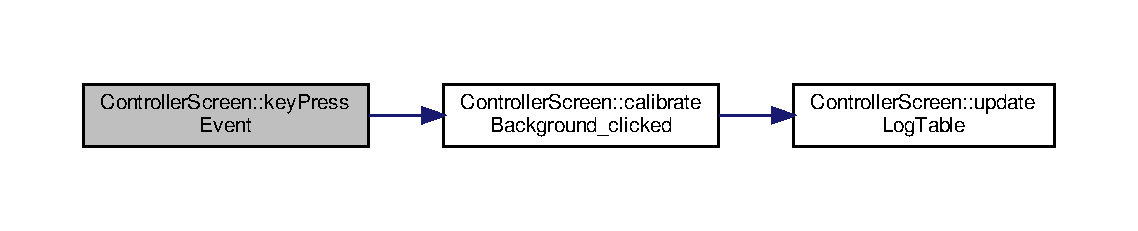
\includegraphics[width=350pt]{class_controller_screen_afbb0033f9be00fce83d54f2a49b9ba89_cgraph}
\end{center}
\end{figure}
\mbox{\Hypertarget{class_controller_screen_ae4d6a51231fb1f6f8809ce3d036592bd}\label{class_controller_screen_ae4d6a51231fb1f6f8809ce3d036592bd}} 
\index{Controller\+Screen@{Controller\+Screen}!set\+Calibration\+Values@{set\+Calibration\+Values}}
\index{set\+Calibration\+Values@{set\+Calibration\+Values}!Controller\+Screen@{Controller\+Screen}}
\subsubsection{\texorpdfstring{set\+Calibration\+Values}{setCalibrationValues}}
{\footnotesize\ttfamily void Controller\+Screen\+::set\+Calibration\+Values (\begin{DoxyParamCaption}{ }\end{DoxyParamCaption})\hspace{0.3cm}{\ttfamily [slot]}}

It sets the calibration values for the signal 

Definition at line 95 of file Controller\+Screen.\+cpp.

Here is the caller graph for this function\+:
\nopagebreak
\begin{figure}[H]
\begin{center}
\leavevmode
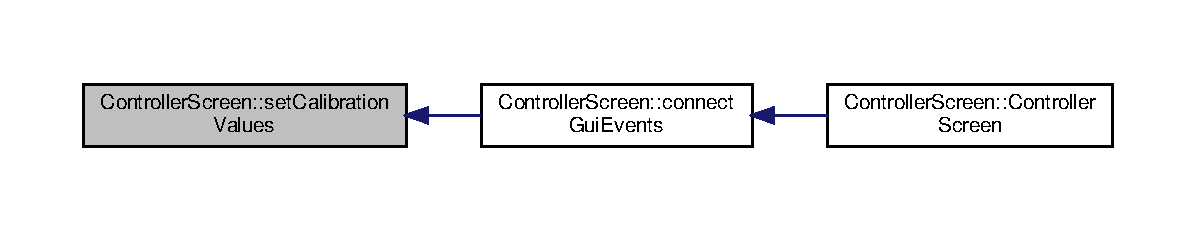
\includegraphics[width=350pt]{class_controller_screen_ae4d6a51231fb1f6f8809ce3d036592bd_icgraph}
\end{center}
\end{figure}
\mbox{\Hypertarget{class_controller_screen_a4d9db4a832f667aacb7d7532f752fd1b}\label{class_controller_screen_a4d9db4a832f667aacb7d7532f752fd1b}} 
\index{Controller\+Screen@{Controller\+Screen}!skin\+Mask\+\_\+clicked@{skin\+Mask\+\_\+clicked}}
\index{skin\+Mask\+\_\+clicked@{skin\+Mask\+\_\+clicked}!Controller\+Screen@{Controller\+Screen}}
\subsubsection{\texorpdfstring{skin\+Mask\+\_\+clicked}{skinMask\_clicked}}
{\footnotesize\ttfamily void Controller\+Screen\+::skin\+Mask\+\_\+clicked (\begin{DoxyParamCaption}{ }\end{DoxyParamCaption})\hspace{0.3cm}{\ttfamily [slot]}}

When the skin\+Mask button is clicked, the image\+View\+Changed signal is emitted with the S\+K\+I\+N\+M\+A\+SK parameter, and the log table is updated. 

Definition at line 65 of file Controller\+Screen.\+cpp.

Here is the call graph for this function\+:
\nopagebreak
\begin{figure}[H]
\begin{center}
\leavevmode
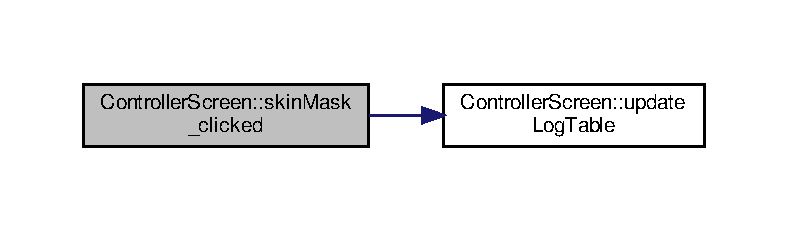
\includegraphics[width=350pt]{class_controller_screen_a4d9db4a832f667aacb7d7532f752fd1b_cgraph}
\end{center}
\end{figure}
Here is the caller graph for this function\+:
\nopagebreak
\begin{figure}[H]
\begin{center}
\leavevmode
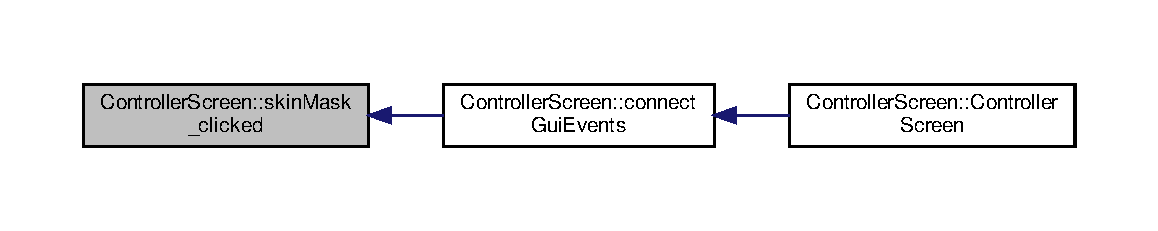
\includegraphics[width=350pt]{class_controller_screen_a4d9db4a832f667aacb7d7532f752fd1b_icgraph}
\end{center}
\end{figure}
\mbox{\Hypertarget{class_controller_screen_aac8b2856372fa02c4f793cf9183dffed}\label{class_controller_screen_aac8b2856372fa02c4f793cf9183dffed}} 
\index{Controller\+Screen@{Controller\+Screen}!unprocessed\+Feed\+\_\+clicked@{unprocessed\+Feed\+\_\+clicked}}
\index{unprocessed\+Feed\+\_\+clicked@{unprocessed\+Feed\+\_\+clicked}!Controller\+Screen@{Controller\+Screen}}
\subsubsection{\texorpdfstring{unprocessed\+Feed\+\_\+clicked}{unprocessedFeed\_clicked}}
{\footnotesize\ttfamily void Controller\+Screen\+::unprocessed\+Feed\+\_\+clicked (\begin{DoxyParamCaption}{ }\end{DoxyParamCaption})\hspace{0.3cm}{\ttfamily [slot]}}

When the unprocessed feed button is clicked, the image view is changed to the unprocessed feed and the log table is updated 

Definition at line 58 of file Controller\+Screen.\+cpp.

Here is the call graph for this function\+:
\nopagebreak
\begin{figure}[H]
\begin{center}
\leavevmode
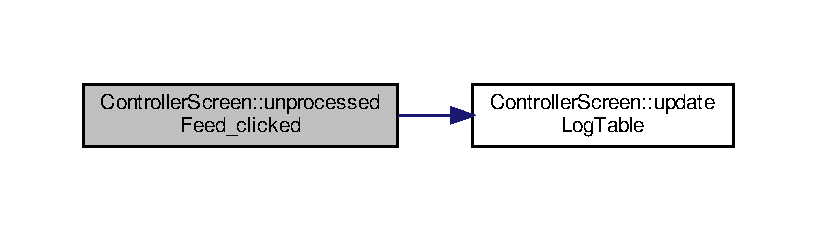
\includegraphics[width=350pt]{class_controller_screen_aac8b2856372fa02c4f793cf9183dffed_cgraph}
\end{center}
\end{figure}
Here is the caller graph for this function\+:
\nopagebreak
\begin{figure}[H]
\begin{center}
\leavevmode
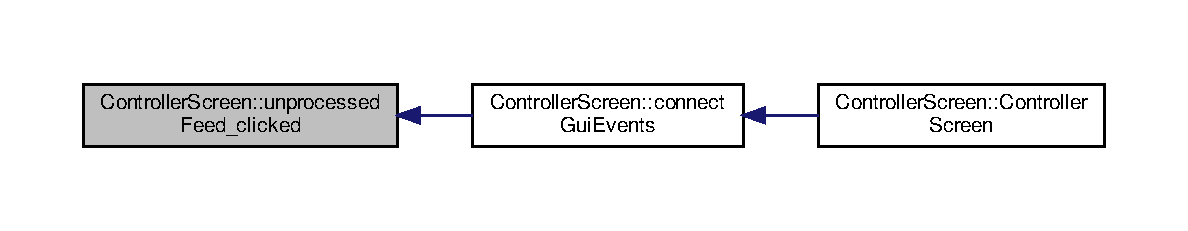
\includegraphics[width=350pt]{class_controller_screen_aac8b2856372fa02c4f793cf9183dffed_icgraph}
\end{center}
\end{figure}
\mbox{\Hypertarget{class_controller_screen_a700c8c1911e68861b86890a5429d2692}\label{class_controller_screen_a700c8c1911e68861b86890a5429d2692}} 
\index{Controller\+Screen@{Controller\+Screen}!update\+Calibrated\+Trackbar@{update\+Calibrated\+Trackbar}}
\index{update\+Calibrated\+Trackbar@{update\+Calibrated\+Trackbar}!Controller\+Screen@{Controller\+Screen}}
\subsubsection{\texorpdfstring{update\+Calibrated\+Trackbar()}{updateCalibratedTrackbar()}}
{\footnotesize\ttfamily void Controller\+Screen\+::update\+Calibrated\+Trackbar (\begin{DoxyParamCaption}\item[{int}]{hmin,  }\item[{int}]{hmax,  }\item[{int}]{smin,  }\item[{int}]{smax }\end{DoxyParamCaption})\hspace{0.3cm}{\ttfamily [override]}, {\ttfamily [virtual]}}

It updates the trackbars on the controller screen with the values passed in


\begin{DoxyParams}{Parameters}
{\em hmin} & minimum hue value \\
\hline
{\em hmax} & Hue maximum value \\
\hline
{\em smin} & minimum saturation value \\
\hline
{\em smax} & The maximum value of the saturation channel. \\
\hline
\end{DoxyParams}


Implements \hyperlink{class_controller_screen_callback_interface_aeee7c043e83e959de0788a9d2a5f70bb}{Controller\+Screen\+Callback\+Interface}.



Definition at line 115 of file Controller\+Screen.\+cpp.

\mbox{\Hypertarget{class_controller_screen_acf75ddc9588011e360e2199cc37478ec}\label{class_controller_screen_acf75ddc9588011e360e2199cc37478ec}} 
\index{Controller\+Screen@{Controller\+Screen}!update\+Image@{update\+Image}}
\index{update\+Image@{update\+Image}!Controller\+Screen@{Controller\+Screen}}
\subsubsection{\texorpdfstring{update\+Image()}{updateImage()}}
{\footnotesize\ttfamily void Controller\+Screen\+::update\+Image (\begin{DoxyParamCaption}\item[{Mat}]{dest }\end{DoxyParamCaption})\hspace{0.3cm}{\ttfamily [override]}}

It recieves the latest frame converts from B\+GR to R\+GB, then it converts the image to a Q\+Image, and finally it sets the Q\+Image to the label


\begin{DoxyParams}{Parameters}
{\em dest} & the image to be displayed \\
\hline
\end{DoxyParams}


Definition at line 109 of file Controller\+Screen.\+cpp.

\mbox{\Hypertarget{class_controller_screen_a039b816adc94fc7e7757520c10fd1d0b}\label{class_controller_screen_a039b816adc94fc7e7757520c10fd1d0b}} 
\index{Controller\+Screen@{Controller\+Screen}!update\+Log\+Table@{update\+Log\+Table}}
\index{update\+Log\+Table@{update\+Log\+Table}!Controller\+Screen@{Controller\+Screen}}
\subsubsection{\texorpdfstring{update\+Log\+Table()}{updateLogTable()}}
{\footnotesize\ttfamily void Controller\+Screen\+::update\+Log\+Table (\begin{DoxyParamCaption}\item[{String}]{a,  }\item[{String}]{b }\end{DoxyParamCaption})\hspace{0.3cm}{\ttfamily [override]}, {\ttfamily [virtual]}}

It takes two strings as arguments, and adds them to the table widget


\begin{DoxyParams}{Parameters}
{\em a} & The first parameter is the name of the function that is being called. \\
\hline
{\em b} & the message to be displayed \\
\hline
\end{DoxyParams}


Implements \hyperlink{class_controller_screen_callback_interface_af92ab0514459c690e357064676fa33f0}{Controller\+Screen\+Callback\+Interface}.



Definition at line 122 of file Controller\+Screen.\+cpp.

Here is the caller graph for this function\+:
\nopagebreak
\begin{figure}[H]
\begin{center}
\leavevmode
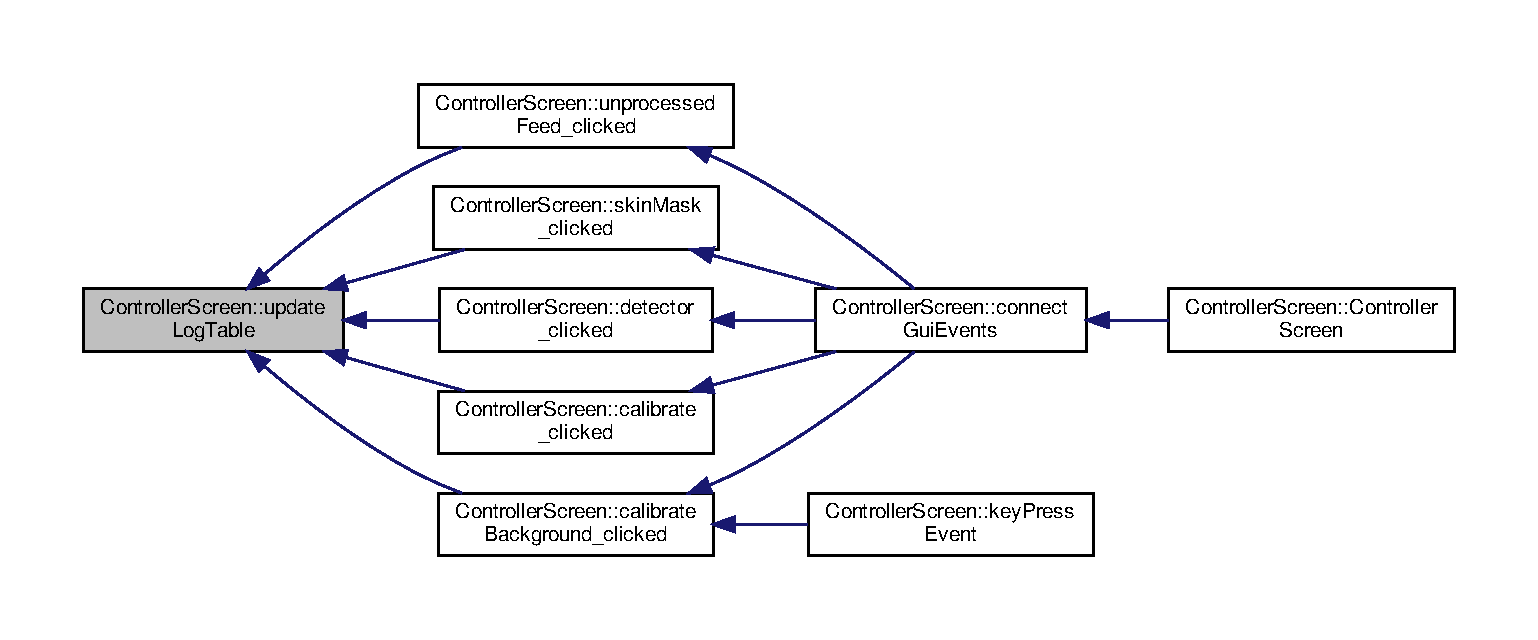
\includegraphics[width=350pt]{class_controller_screen_a039b816adc94fc7e7757520c10fd1d0b_icgraph}
\end{center}
\end{figure}


\subsection{Member Data Documentation}
\mbox{\Hypertarget{class_controller_screen_a672477c37c55499b69e28da611e7313d}\label{class_controller_screen_a672477c37c55499b69e28da611e7313d}} 
\index{Controller\+Screen@{Controller\+Screen}!capture\+And\+Detect@{capture\+And\+Detect}}
\index{capture\+And\+Detect@{capture\+And\+Detect}!Controller\+Screen@{Controller\+Screen}}
\subsubsection{\texorpdfstring{capture\+And\+Detect}{captureAndDetect}}
{\footnotesize\ttfamily \hyperlink{class_gestro_1_1_capture_and_detect}{Capture\+And\+Detect} Controller\+Screen\+::capture\+And\+Detect\hspace{0.3cm}{\ttfamily [private]}}



Creating an instance of the Capture\+And\+Detect class. 



Definition at line 94 of file Controller\+Screen.\+h.

\mbox{\Hypertarget{class_controller_screen_a240495b9e446bc512d8a7498b3f45981}\label{class_controller_screen_a240495b9e446bc512d8a7498b3f45981}} 
\index{Controller\+Screen@{Controller\+Screen}!display@{display}}
\index{display@{display}!Controller\+Screen@{Controller\+Screen}}
\subsubsection{\texorpdfstring{display}{display}}
{\footnotesize\ttfamily Display$\ast$ Controller\+Screen\+::display = X\+Open\+Display(N\+U\+LL)\hspace{0.3cm}{\ttfamily [private]}}



Opening a connection to the X server. 



Definition at line 97 of file Controller\+Screen.\+h.

\mbox{\Hypertarget{class_controller_screen_a261f7eb9894dbcfdbddad62ad125e330}\label{class_controller_screen_a261f7eb9894dbcfdbddad62ad125e330}} 
\index{Controller\+Screen@{Controller\+Screen}!display\+Control@{display\+Control}}
\index{display\+Control@{display\+Control}!Controller\+Screen@{Controller\+Screen}}
\subsubsection{\texorpdfstring{display\+Control}{displayControl}}
{\footnotesize\ttfamily \hyperlink{class_gestro_1_1_display_control}{Display\+Control} Controller\+Screen\+::display\+Control = \hyperlink{class_gestro_1_1_display_control}{Display\+Control}(\hyperlink{class_controller_screen_a240495b9e446bc512d8a7498b3f45981}{display})\hspace{0.3cm}{\ttfamily [private]}}



Creating an instance of the Display\+Control class. 



Definition at line 100 of file Controller\+Screen.\+h.

\mbox{\Hypertarget{class_controller_screen_a96533700d5a3a0593d9b9d24a724b16b}\label{class_controller_screen_a96533700d5a3a0593d9b9d24a724b16b}} 
\index{Controller\+Screen@{Controller\+Screen}!enabled\+Commands@{enabled\+Commands}}
\index{enabled\+Commands@{enabled\+Commands}!Controller\+Screen@{Controller\+Screen}}
\subsubsection{\texorpdfstring{enabled\+Commands}{enabledCommands}}
{\footnotesize\ttfamily \hyperlink{class_gesture_detection_1_1_enabled_command}{Enabled\+Command} Controller\+Screen\+::enabled\+Commands\hspace{0.3cm}{\ttfamily [private]}}



A class that is used to store the enabled commands. 



Definition at line 109 of file Controller\+Screen.\+h.

\mbox{\Hypertarget{class_controller_screen_ae667566a3438ae194170858cd328053e}\label{class_controller_screen_ae667566a3438ae194170858cd328053e}} 
\index{Controller\+Screen@{Controller\+Screen}!screen@{screen}}
\index{screen@{screen}!Controller\+Screen@{Controller\+Screen}}
\subsubsection{\texorpdfstring{screen}{screen}}
{\footnotesize\ttfamily Screen$\ast$ Controller\+Screen\+::screen = Default\+Screen\+Of\+Display(\hyperlink{class_controller_screen_a240495b9e446bc512d8a7498b3f45981}{display})\hspace{0.3cm}{\ttfamily [private]}}



Getting the default screen of the display. 



Definition at line 103 of file Controller\+Screen.\+h.

\mbox{\Hypertarget{class_controller_screen_afe5953fdc933fcc35cf0ef841c83f18c}\label{class_controller_screen_afe5953fdc933fcc35cf0ef841c83f18c}} 
\index{Controller\+Screen@{Controller\+Screen}!signal@{signal}}
\index{signal@{signal}!Controller\+Screen@{Controller\+Screen}}
\subsubsection{\texorpdfstring{signal}{signal}}
{\footnotesize\ttfamily \hyperlink{struct_custom_signals}{Custom\+Signals} Controller\+Screen\+::signal\hspace{0.3cm}{\ttfamily [private]}}



Creating an instance of the \hyperlink{struct_custom_signals}{Custom\+Signals} class. 



Definition at line 106 of file Controller\+Screen.\+h.

\mbox{\Hypertarget{class_controller_screen_a25a37166616a171730a89ddb69c120f3}\label{class_controller_screen_a25a37166616a171730a89ddb69c120f3}} 
\index{Controller\+Screen@{Controller\+Screen}!ui@{ui}}
\index{ui@{ui}!Controller\+Screen@{Controller\+Screen}}
\subsubsection{\texorpdfstring{ui}{ui}}
{\footnotesize\ttfamily Ui\+::\+Controller\+Screen$\ast$ Controller\+Screen\+::ui\hspace{0.3cm}{\ttfamily [private]}}



A pointer to the ui class. 



Definition at line 91 of file Controller\+Screen.\+h.



The documentation for this class was generated from the following files\+:\begin{DoxyCompactItemize}
\item 
src/gui/\hyperlink{_controller_screen_8h}{Controller\+Screen.\+h}\item 
src/gui/\hyperlink{_controller_screen_8cpp}{Controller\+Screen.\+cpp}\end{DoxyCompactItemize}

\hypertarget{class_controller_screen_callback_interface}{}\section{Controller\+Screen\+Callback\+Interface Class Reference}
\label{class_controller_screen_callback_interface}\index{Controller\+Screen\+Callback\+Interface@{Controller\+Screen\+Callback\+Interface}}


Callback interface to \hyperlink{class_controller_screen}{Controller\+Screen}.  




{\ttfamily \#include $<$Controller\+Screen\+Callback\+Interface.\+h$>$}



Inheritance diagram for Controller\+Screen\+Callback\+Interface\+:
\nopagebreak
\begin{figure}[H]
\begin{center}
\leavevmode
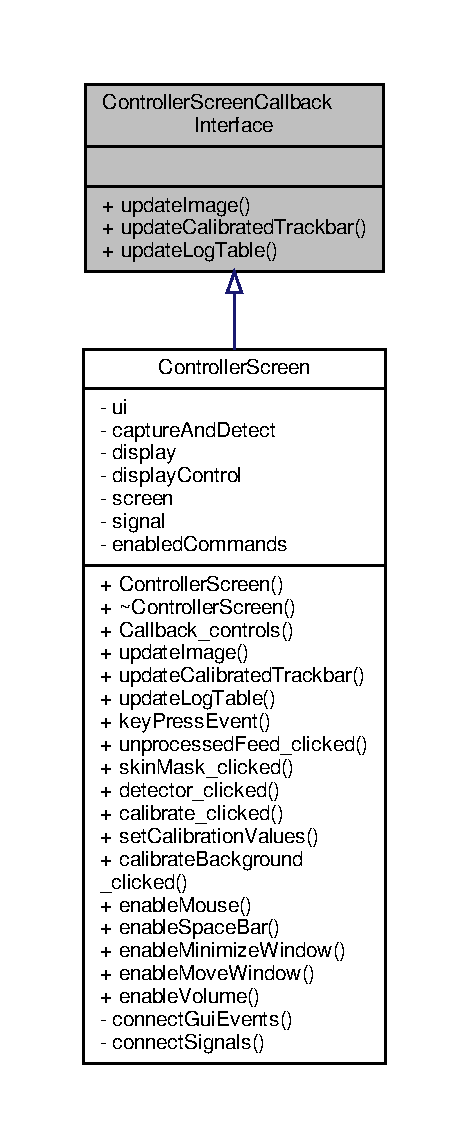
\includegraphics[height=550pt]{class_controller_screen_callback_interface__inherit__graph}
\end{center}
\end{figure}


Collaboration diagram for Controller\+Screen\+Callback\+Interface\+:
\nopagebreak
\begin{figure}[H]
\begin{center}
\leavevmode
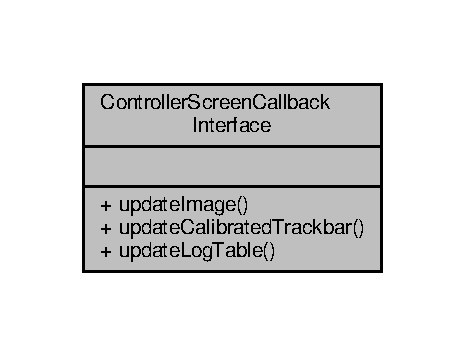
\includegraphics[width=223pt]{class_controller_screen_callback_interface__coll__graph}
\end{center}
\end{figure}
\subsection*{Public Member Functions}
\begin{DoxyCompactItemize}
\item 
virtual void \hyperlink{class_controller_screen_callback_interface_a7d11a5d40ead88e7f89b8b1ee836b0cd}{update\+Image} (cv\+::\+Mat)=0
\item 
virtual void \hyperlink{class_controller_screen_callback_interface_aeee7c043e83e959de0788a9d2a5f70bb}{update\+Calibrated\+Trackbar} (int, int, int, int)=0
\item 
virtual void \hyperlink{class_controller_screen_callback_interface_af92ab0514459c690e357064676fa33f0}{update\+Log\+Table} (String a, String b)=0
\end{DoxyCompactItemize}


\subsection{Detailed Description}
Callback interface to \hyperlink{class_controller_screen}{Controller\+Screen}. 

Definition at line 7 of file Controller\+Screen\+Callback\+Interface.\+h.



\subsection{Member Function Documentation}
\mbox{\Hypertarget{class_controller_screen_callback_interface_aeee7c043e83e959de0788a9d2a5f70bb}\label{class_controller_screen_callback_interface_aeee7c043e83e959de0788a9d2a5f70bb}} 
\index{Controller\+Screen\+Callback\+Interface@{Controller\+Screen\+Callback\+Interface}!update\+Calibrated\+Trackbar@{update\+Calibrated\+Trackbar}}
\index{update\+Calibrated\+Trackbar@{update\+Calibrated\+Trackbar}!Controller\+Screen\+Callback\+Interface@{Controller\+Screen\+Callback\+Interface}}
\subsubsection{\texorpdfstring{update\+Calibrated\+Trackbar()}{updateCalibratedTrackbar()}}
{\footnotesize\ttfamily virtual void Controller\+Screen\+Callback\+Interface\+::update\+Calibrated\+Trackbar (\begin{DoxyParamCaption}\item[{int}]{,  }\item[{int}]{,  }\item[{int}]{,  }\item[{int}]{ }\end{DoxyParamCaption})\hspace{0.3cm}{\ttfamily [pure virtual]}}



Implemented in \hyperlink{class_controller_screen_a700c8c1911e68861b86890a5429d2692}{Controller\+Screen}.

Here is the caller graph for this function\+:
\nopagebreak
\begin{figure}[H]
\begin{center}
\leavevmode
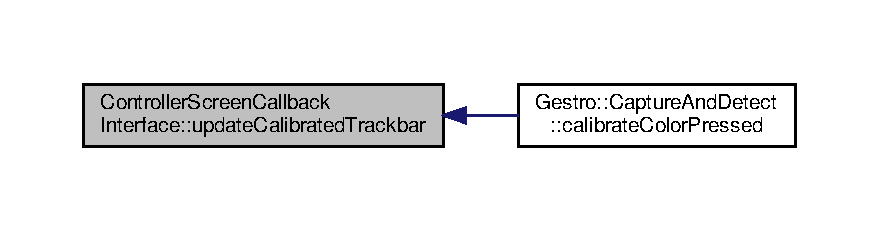
\includegraphics[width=350pt]{class_controller_screen_callback_interface_aeee7c043e83e959de0788a9d2a5f70bb_icgraph}
\end{center}
\end{figure}
\mbox{\Hypertarget{class_controller_screen_callback_interface_a7d11a5d40ead88e7f89b8b1ee836b0cd}\label{class_controller_screen_callback_interface_a7d11a5d40ead88e7f89b8b1ee836b0cd}} 
\index{Controller\+Screen\+Callback\+Interface@{Controller\+Screen\+Callback\+Interface}!update\+Image@{update\+Image}}
\index{update\+Image@{update\+Image}!Controller\+Screen\+Callback\+Interface@{Controller\+Screen\+Callback\+Interface}}
\subsubsection{\texorpdfstring{update\+Image()}{updateImage()}}
{\footnotesize\ttfamily virtual void Controller\+Screen\+Callback\+Interface\+::update\+Image (\begin{DoxyParamCaption}\item[{cv\+::\+Mat}]{ }\end{DoxyParamCaption})\hspace{0.3cm}{\ttfamily [pure virtual]}}

Here is the caller graph for this function\+:
\nopagebreak
\begin{figure}[H]
\begin{center}
\leavevmode
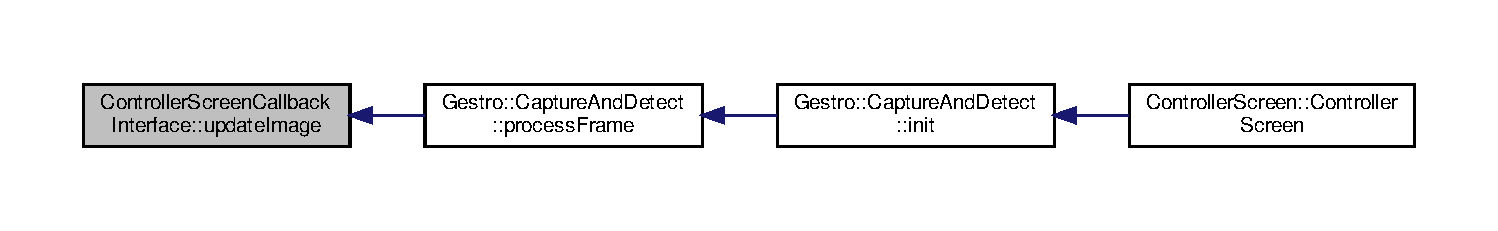
\includegraphics[width=350pt]{class_controller_screen_callback_interface_a7d11a5d40ead88e7f89b8b1ee836b0cd_icgraph}
\end{center}
\end{figure}
\mbox{\Hypertarget{class_controller_screen_callback_interface_af92ab0514459c690e357064676fa33f0}\label{class_controller_screen_callback_interface_af92ab0514459c690e357064676fa33f0}} 
\index{Controller\+Screen\+Callback\+Interface@{Controller\+Screen\+Callback\+Interface}!update\+Log\+Table@{update\+Log\+Table}}
\index{update\+Log\+Table@{update\+Log\+Table}!Controller\+Screen\+Callback\+Interface@{Controller\+Screen\+Callback\+Interface}}
\subsubsection{\texorpdfstring{update\+Log\+Table()}{updateLogTable()}}
{\footnotesize\ttfamily virtual void Controller\+Screen\+Callback\+Interface\+::update\+Log\+Table (\begin{DoxyParamCaption}\item[{String}]{a,  }\item[{String}]{b }\end{DoxyParamCaption})\hspace{0.3cm}{\ttfamily [pure virtual]}}



Implemented in \hyperlink{class_controller_screen_a039b816adc94fc7e7757520c10fd1d0b}{Controller\+Screen}.



The documentation for this class was generated from the following file\+:\begin{DoxyCompactItemize}
\item 
src/gui/\hyperlink{_controller_screen_callback_interface_8h}{Controller\+Screen\+Callback\+Interface.\+h}\end{DoxyCompactItemize}

\hypertarget{struct_custom_signals}{}\section{Custom\+Signals Struct Reference}
\label{struct_custom_signals}\index{Custom\+Signals@{Custom\+Signals}}


Stored signals to connect to.  




{\ttfamily \#include $<$Custom\+Signals.\+h$>$}



Collaboration diagram for Custom\+Signals\+:
\nopagebreak
\begin{figure}[H]
\begin{center}
\leavevmode
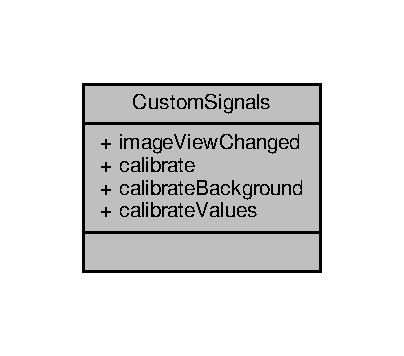
\includegraphics[width=194pt]{struct_custom_signals__coll__graph}
\end{center}
\end{figure}
\subsection*{Public Attributes}
\begin{DoxyCompactItemize}
\item 
boost\+::signals2\+::signal$<$ void(\hyperlink{_capture_and_detect_8h_a425a93be55e757f5e351ec9d6770c50e}{Feed})$>$ \hyperlink{struct_custom_signals_ac453891590a3536656f21a5ef55efcbe}{image\+View\+Changed}
\item 
boost\+::signals2\+::signal$<$ void()$>$ \hyperlink{struct_custom_signals_affeb9cf3ae6f465af657b9e13f2f51e6}{calibrate}
\item 
boost\+::signals2\+::signal$<$ void()$>$ \hyperlink{struct_custom_signals_aa853ceb0f87d27fb4d8318b98a5e36c6}{calibrate\+Background}
\item 
boost\+::signals2\+::signal$<$ void(int, int, int, int)$>$ \hyperlink{struct_custom_signals_a9383d26c828ce25b99c0a64fc8adcdc2}{calibrate\+Values}
\end{DoxyCompactItemize}


\subsection{Detailed Description}
Stored signals to connect to. 

Definition at line 7 of file Custom\+Signals.\+h.



\subsection{Member Data Documentation}
\mbox{\Hypertarget{struct_custom_signals_affeb9cf3ae6f465af657b9e13f2f51e6}\label{struct_custom_signals_affeb9cf3ae6f465af657b9e13f2f51e6}} 
\index{Custom\+Signals@{Custom\+Signals}!calibrate@{calibrate}}
\index{calibrate@{calibrate}!Custom\+Signals@{Custom\+Signals}}
\subsubsection{\texorpdfstring{calibrate}{calibrate}}
{\footnotesize\ttfamily boost\+::signals2\+::signal$<$void()$>$ Custom\+Signals\+::calibrate}



Definition at line 9 of file Custom\+Signals.\+h.

\mbox{\Hypertarget{struct_custom_signals_aa853ceb0f87d27fb4d8318b98a5e36c6}\label{struct_custom_signals_aa853ceb0f87d27fb4d8318b98a5e36c6}} 
\index{Custom\+Signals@{Custom\+Signals}!calibrate\+Background@{calibrate\+Background}}
\index{calibrate\+Background@{calibrate\+Background}!Custom\+Signals@{Custom\+Signals}}
\subsubsection{\texorpdfstring{calibrate\+Background}{calibrateBackground}}
{\footnotesize\ttfamily boost\+::signals2\+::signal$<$void()$>$ Custom\+Signals\+::calibrate\+Background}



Definition at line 10 of file Custom\+Signals.\+h.

\mbox{\Hypertarget{struct_custom_signals_a9383d26c828ce25b99c0a64fc8adcdc2}\label{struct_custom_signals_a9383d26c828ce25b99c0a64fc8adcdc2}} 
\index{Custom\+Signals@{Custom\+Signals}!calibrate\+Values@{calibrate\+Values}}
\index{calibrate\+Values@{calibrate\+Values}!Custom\+Signals@{Custom\+Signals}}
\subsubsection{\texorpdfstring{calibrate\+Values}{calibrateValues}}
{\footnotesize\ttfamily boost\+::signals2\+::signal$<$void(int,int,int,int)$>$ Custom\+Signals\+::calibrate\+Values}



Definition at line 11 of file Custom\+Signals.\+h.

\mbox{\Hypertarget{struct_custom_signals_ac453891590a3536656f21a5ef55efcbe}\label{struct_custom_signals_ac453891590a3536656f21a5ef55efcbe}} 
\index{Custom\+Signals@{Custom\+Signals}!image\+View\+Changed@{image\+View\+Changed}}
\index{image\+View\+Changed@{image\+View\+Changed}!Custom\+Signals@{Custom\+Signals}}
\subsubsection{\texorpdfstring{image\+View\+Changed}{imageViewChanged}}
{\footnotesize\ttfamily boost\+::signals2\+::signal$<$void(\hyperlink{_capture_and_detect_8h_a425a93be55e757f5e351ec9d6770c50e}{Feed})$>$ Custom\+Signals\+::image\+View\+Changed}



Definition at line 8 of file Custom\+Signals.\+h.



The documentation for this struct was generated from the following file\+:\begin{DoxyCompactItemize}
\item 
src/gui/\hyperlink{_custom_signals_8h}{Custom\+Signals.\+h}\end{DoxyCompactItemize}

\hypertarget{class_gestro_1_1_display_control}{}\section{Gestro\+:\+:Display\+Control Class Reference}
\label{class_gestro_1_1_display_control}\index{Gestro\+::\+Display\+Control@{Gestro\+::\+Display\+Control}}


This is a class that is inheriting from the classes Window\+Action, Keyboard\+Action, Mouse\+Action, Volume\+Control, and \hyperlink{class_gestro_1_1_display_control_callback_interface}{Display\+Control\+Callback\+Interface}.  




{\ttfamily \#include $<$Display\+Control.\+h$>$}



Inheritance diagram for Gestro\+:\+:Display\+Control\+:
\nopagebreak
\begin{figure}[H]
\begin{center}
\leavevmode
\includegraphics[width=350pt]{class_gestro_1_1_display_control__inherit__graph}
\end{center}
\end{figure}


Collaboration diagram for Gestro\+:\+:Display\+Control\+:
\nopagebreak
\begin{figure}[H]
\begin{center}
\leavevmode
\includegraphics[width=350pt]{class_gestro_1_1_display_control__coll__graph}
\end{center}
\end{figure}
\subsection*{Public Member Functions}
\begin{DoxyCompactItemize}
\item 
\hyperlink{class_gestro_1_1_display_control_a4d2a5053b250bbd1f3103795cb29fcde}{Display\+Control} (Display $\ast$d)
\item 
void \hyperlink{class_gestro_1_1_display_control_aa8c509a1e17ba12d164dcfe43cf281d4}{do\+Mouse\+Move} (int, int) override
\item 
void \hyperlink{class_gestro_1_1_display_control_aa5af48425f7ba40012b2a7db5fabed45}{do\+Key\+Press} (int) override
\item 
void \hyperlink{class_gestro_1_1_display_control_a8a361b4c25ef55b86b5c2d178ffa516f}{do\+Increase\+Volume} () override
\item 
void \hyperlink{class_gestro_1_1_display_control_a874fa3f6b3e4cf465db62a4eba1c1dd1}{do\+Reduce\+Volume} () override
\item 
void \hyperlink{class_gestro_1_1_display_control_a210411b559d8c3ffb1498f49cfa26a6d}{do\+Unmute} () override
\item 
void \hyperlink{class_gestro_1_1_display_control_a25f685ea6bf001e53c7d17410f2a24ea}{do\+Mute\+Unmute} () override
\item 
void \hyperlink{class_gestro_1_1_display_control_a5f45c36e699afa1d56b2af78e5125aca}{do\+Button\+Press} (int) override
\item 
void \hyperlink{class_gestro_1_1_display_control_aca4208c53cac28e164e7949effdc04cd}{do\+Window\+Move} (int, int) override
\item 
void \hyperlink{class_gestro_1_1_display_control_ad5fa763a77c680ce7b2089c6d79c4eb7}{do\+Window\+Minimize} () override
\end{DoxyCompactItemize}
\subsection*{Private Attributes}
\begin{DoxyCompactItemize}
\item 
Display $\ast$ \hyperlink{class_gestro_1_1_display_control_a6a6844fa13ff67a20596cacd8c5c52d8}{display}
\begin{DoxyCompactList}\small\item\em A pointer to the display variable. \end{DoxyCompactList}\item 
X\+Event \hyperlink{class_gestro_1_1_display_control_a1bf9a5a6abafb845fe5bbeb7e84f715d}{event}
\begin{DoxyCompactList}\small\item\em A variable that is used to store the event that is being passed to the callback function. \end{DoxyCompactList}\end{DoxyCompactItemize}


\subsection{Detailed Description}
This is a class that is inheriting from the classes Window\+Action, Keyboard\+Action, Mouse\+Action, Volume\+Control, and \hyperlink{class_gestro_1_1_display_control_callback_interface}{Display\+Control\+Callback\+Interface}. 

This class is used in order to concisely encapsulate the classes for keyboard,window, mouse and volume control into a single class so that they can be used in a callback function without the user needing to create objects for each of those classes any of the methods from the parent classes can be called by simply using dot notation 

Definition at line 23 of file Display\+Control.\+h.



\subsection{Constructor \& Destructor Documentation}
\mbox{\Hypertarget{class_gestro_1_1_display_control_a4d2a5053b250bbd1f3103795cb29fcde}\label{class_gestro_1_1_display_control_a4d2a5053b250bbd1f3103795cb29fcde}} 
\index{Gestro\+::\+Display\+Control@{Gestro\+::\+Display\+Control}!Display\+Control@{Display\+Control}}
\index{Display\+Control@{Display\+Control}!Gestro\+::\+Display\+Control@{Gestro\+::\+Display\+Control}}
\subsubsection{\texorpdfstring{Display\+Control()}{DisplayControl()}}
{\footnotesize\ttfamily Display\+Control\+::\+Display\+Control (\begin{DoxyParamCaption}\item[{Display $\ast$}]{d }\end{DoxyParamCaption})}

Constructor that takes in a display variable


\begin{DoxyParams}{Parameters}
{\em d} & The display to use. \\
\hline
\end{DoxyParams}


Definition at line 5 of file Display\+Control.\+cpp.



\subsection{Member Function Documentation}
\mbox{\Hypertarget{class_gestro_1_1_display_control_a5f45c36e699afa1d56b2af78e5125aca}\label{class_gestro_1_1_display_control_a5f45c36e699afa1d56b2af78e5125aca}} 
\index{Gestro\+::\+Display\+Control@{Gestro\+::\+Display\+Control}!do\+Button\+Press@{do\+Button\+Press}}
\index{do\+Button\+Press@{do\+Button\+Press}!Gestro\+::\+Display\+Control@{Gestro\+::\+Display\+Control}}
\subsubsection{\texorpdfstring{do\+Button\+Press()}{doButtonPress()}}
{\footnotesize\ttfamily void Display\+Control\+::do\+Button\+Press (\begin{DoxyParamCaption}\item[{int}]{x }\end{DoxyParamCaption})\hspace{0.3cm}{\ttfamily [override]}, {\ttfamily [virtual]}}

overrides the Display\+Control\+Interface method and uses Mouse\+Action to press\+Button 

Implements \hyperlink{class_gestro_1_1_display_control_callback_interface_ab661600cad2743fd41253fb9cabbee51}{Gestro\+::\+Display\+Control\+Callback\+Interface}.



Definition at line 33 of file Display\+Control.\+cpp.

Here is the call graph for this function\+:
\nopagebreak
\begin{figure}[H]
\begin{center}
\leavevmode
\includegraphics[width=350pt]{class_gestro_1_1_display_control_a5f45c36e699afa1d56b2af78e5125aca_cgraph}
\end{center}
\end{figure}
\mbox{\Hypertarget{class_gestro_1_1_display_control_a8a361b4c25ef55b86b5c2d178ffa516f}\label{class_gestro_1_1_display_control_a8a361b4c25ef55b86b5c2d178ffa516f}} 
\index{Gestro\+::\+Display\+Control@{Gestro\+::\+Display\+Control}!do\+Increase\+Volume@{do\+Increase\+Volume}}
\index{do\+Increase\+Volume@{do\+Increase\+Volume}!Gestro\+::\+Display\+Control@{Gestro\+::\+Display\+Control}}
\subsubsection{\texorpdfstring{do\+Increase\+Volume()}{doIncreaseVolume()}}
{\footnotesize\ttfamily void Display\+Control\+::do\+Increase\+Volume (\begin{DoxyParamCaption}{ }\end{DoxyParamCaption})\hspace{0.3cm}{\ttfamily [override]}, {\ttfamily [virtual]}}

overrides the Display\+Control\+Interface method and uses Volume\+Control to increase\+Volume 

Implements \hyperlink{class_gestro_1_1_display_control_callback_interface_af26f63171de9622c5723363732f590c8}{Gestro\+::\+Display\+Control\+Callback\+Interface}.



Definition at line 17 of file Display\+Control.\+cpp.

Here is the call graph for this function\+:
\nopagebreak
\begin{figure}[H]
\begin{center}
\leavevmode
\includegraphics[width=350pt]{class_gestro_1_1_display_control_a8a361b4c25ef55b86b5c2d178ffa516f_cgraph}
\end{center}
\end{figure}
\mbox{\Hypertarget{class_gestro_1_1_display_control_aa5af48425f7ba40012b2a7db5fabed45}\label{class_gestro_1_1_display_control_aa5af48425f7ba40012b2a7db5fabed45}} 
\index{Gestro\+::\+Display\+Control@{Gestro\+::\+Display\+Control}!do\+Key\+Press@{do\+Key\+Press}}
\index{do\+Key\+Press@{do\+Key\+Press}!Gestro\+::\+Display\+Control@{Gestro\+::\+Display\+Control}}
\subsubsection{\texorpdfstring{do\+Key\+Press()}{doKeyPress()}}
{\footnotesize\ttfamily void Display\+Control\+::do\+Key\+Press (\begin{DoxyParamCaption}\item[{int}]{x }\end{DoxyParamCaption})\hspace{0.3cm}{\ttfamily [override]}, {\ttfamily [virtual]}}

overrides the Display\+Control\+Interface method and uses Keyboard\+Action to press\+Key 

Implements \hyperlink{class_gestro_1_1_display_control_callback_interface_aa6d1e75bb4b3aa0b0e10497576b1053f}{Gestro\+::\+Display\+Control\+Callback\+Interface}.



Definition at line 13 of file Display\+Control.\+cpp.

Here is the call graph for this function\+:
\nopagebreak
\begin{figure}[H]
\begin{center}
\leavevmode
\includegraphics[width=350pt]{class_gestro_1_1_display_control_aa5af48425f7ba40012b2a7db5fabed45_cgraph}
\end{center}
\end{figure}
\mbox{\Hypertarget{class_gestro_1_1_display_control_aa8c509a1e17ba12d164dcfe43cf281d4}\label{class_gestro_1_1_display_control_aa8c509a1e17ba12d164dcfe43cf281d4}} 
\index{Gestro\+::\+Display\+Control@{Gestro\+::\+Display\+Control}!do\+Mouse\+Move@{do\+Mouse\+Move}}
\index{do\+Mouse\+Move@{do\+Mouse\+Move}!Gestro\+::\+Display\+Control@{Gestro\+::\+Display\+Control}}
\subsubsection{\texorpdfstring{do\+Mouse\+Move()}{doMouseMove()}}
{\footnotesize\ttfamily void Display\+Control\+::do\+Mouse\+Move (\begin{DoxyParamCaption}\item[{int}]{x,  }\item[{int}]{y }\end{DoxyParamCaption})\hspace{0.3cm}{\ttfamily [override]}, {\ttfamily [virtual]}}

overrides the Display\+Control\+Interface method and uses Mouse\+Action to move\+Mouse 

Implements \hyperlink{class_gestro_1_1_display_control_callback_interface_a35d453c78b578d061c89c95b3ae9ee8a}{Gestro\+::\+Display\+Control\+Callback\+Interface}.



Definition at line 9 of file Display\+Control.\+cpp.

Here is the call graph for this function\+:
\nopagebreak
\begin{figure}[H]
\begin{center}
\leavevmode
\includegraphics[width=350pt]{class_gestro_1_1_display_control_aa8c509a1e17ba12d164dcfe43cf281d4_cgraph}
\end{center}
\end{figure}
\mbox{\Hypertarget{class_gestro_1_1_display_control_a25f685ea6bf001e53c7d17410f2a24ea}\label{class_gestro_1_1_display_control_a25f685ea6bf001e53c7d17410f2a24ea}} 
\index{Gestro\+::\+Display\+Control@{Gestro\+::\+Display\+Control}!do\+Mute\+Unmute@{do\+Mute\+Unmute}}
\index{do\+Mute\+Unmute@{do\+Mute\+Unmute}!Gestro\+::\+Display\+Control@{Gestro\+::\+Display\+Control}}
\subsubsection{\texorpdfstring{do\+Mute\+Unmute()}{doMuteUnmute()}}
{\footnotesize\ttfamily void Display\+Control\+::do\+Mute\+Unmute (\begin{DoxyParamCaption}{ }\end{DoxyParamCaption})\hspace{0.3cm}{\ttfamily [override]}, {\ttfamily [virtual]}}

overrides the Display\+Control\+Interface method and uses Volume\+Control to mute\+Unmute\+Volume 

Implements \hyperlink{class_gestro_1_1_display_control_callback_interface_ab660632d549760b0404388fc8e86714a}{Gestro\+::\+Display\+Control\+Callback\+Interface}.



Definition at line 25 of file Display\+Control.\+cpp.

Here is the call graph for this function\+:
\nopagebreak
\begin{figure}[H]
\begin{center}
\leavevmode
\includegraphics[width=350pt]{class_gestro_1_1_display_control_a25f685ea6bf001e53c7d17410f2a24ea_cgraph}
\end{center}
\end{figure}
\mbox{\Hypertarget{class_gestro_1_1_display_control_a874fa3f6b3e4cf465db62a4eba1c1dd1}\label{class_gestro_1_1_display_control_a874fa3f6b3e4cf465db62a4eba1c1dd1}} 
\index{Gestro\+::\+Display\+Control@{Gestro\+::\+Display\+Control}!do\+Reduce\+Volume@{do\+Reduce\+Volume}}
\index{do\+Reduce\+Volume@{do\+Reduce\+Volume}!Gestro\+::\+Display\+Control@{Gestro\+::\+Display\+Control}}
\subsubsection{\texorpdfstring{do\+Reduce\+Volume()}{doReduceVolume()}}
{\footnotesize\ttfamily void Display\+Control\+::do\+Reduce\+Volume (\begin{DoxyParamCaption}{ }\end{DoxyParamCaption})\hspace{0.3cm}{\ttfamily [override]}, {\ttfamily [virtual]}}

overrides the Display\+Control\+Interface method and uses Volume\+Control to reduce\+Volume 

Implements \hyperlink{class_gestro_1_1_display_control_callback_interface_a8648fb64585379393917e6b50e348070}{Gestro\+::\+Display\+Control\+Callback\+Interface}.



Definition at line 21 of file Display\+Control.\+cpp.

Here is the call graph for this function\+:
\nopagebreak
\begin{figure}[H]
\begin{center}
\leavevmode
\includegraphics[width=350pt]{class_gestro_1_1_display_control_a874fa3f6b3e4cf465db62a4eba1c1dd1_cgraph}
\end{center}
\end{figure}
\mbox{\Hypertarget{class_gestro_1_1_display_control_a210411b559d8c3ffb1498f49cfa26a6d}\label{class_gestro_1_1_display_control_a210411b559d8c3ffb1498f49cfa26a6d}} 
\index{Gestro\+::\+Display\+Control@{Gestro\+::\+Display\+Control}!do\+Unmute@{do\+Unmute}}
\index{do\+Unmute@{do\+Unmute}!Gestro\+::\+Display\+Control@{Gestro\+::\+Display\+Control}}
\subsubsection{\texorpdfstring{do\+Unmute()}{doUnmute()}}
{\footnotesize\ttfamily void Display\+Control\+::do\+Unmute (\begin{DoxyParamCaption}{ }\end{DoxyParamCaption})\hspace{0.3cm}{\ttfamily [override]}, {\ttfamily [virtual]}}

overrides the Display\+Control\+Interface method and uses Volume\+Control to unmute\+Volume 

Implements \hyperlink{class_gestro_1_1_display_control_callback_interface_a74ddca7b1ef399a41f6025163407bb4d}{Gestro\+::\+Display\+Control\+Callback\+Interface}.



Definition at line 29 of file Display\+Control.\+cpp.

Here is the call graph for this function\+:
\nopagebreak
\begin{figure}[H]
\begin{center}
\leavevmode
\includegraphics[width=350pt]{class_gestro_1_1_display_control_a210411b559d8c3ffb1498f49cfa26a6d_cgraph}
\end{center}
\end{figure}
\mbox{\Hypertarget{class_gestro_1_1_display_control_ad5fa763a77c680ce7b2089c6d79c4eb7}\label{class_gestro_1_1_display_control_ad5fa763a77c680ce7b2089c6d79c4eb7}} 
\index{Gestro\+::\+Display\+Control@{Gestro\+::\+Display\+Control}!do\+Window\+Minimize@{do\+Window\+Minimize}}
\index{do\+Window\+Minimize@{do\+Window\+Minimize}!Gestro\+::\+Display\+Control@{Gestro\+::\+Display\+Control}}
\subsubsection{\texorpdfstring{do\+Window\+Minimize()}{doWindowMinimize()}}
{\footnotesize\ttfamily void Display\+Control\+::do\+Window\+Minimize (\begin{DoxyParamCaption}{ }\end{DoxyParamCaption})\hspace{0.3cm}{\ttfamily [override]}, {\ttfamily [virtual]}}

overrides the Display\+Control\+Interface method and uses Window\+Action to minimize\+Window 

Implements \hyperlink{class_gestro_1_1_display_control_callback_interface_a677aa306f08c548396a048c680bf5e10}{Gestro\+::\+Display\+Control\+Callback\+Interface}.



Definition at line 41 of file Display\+Control.\+cpp.

Here is the call graph for this function\+:
\nopagebreak
\begin{figure}[H]
\begin{center}
\leavevmode
\includegraphics[width=350pt]{class_gestro_1_1_display_control_ad5fa763a77c680ce7b2089c6d79c4eb7_cgraph}
\end{center}
\end{figure}
\mbox{\Hypertarget{class_gestro_1_1_display_control_aca4208c53cac28e164e7949effdc04cd}\label{class_gestro_1_1_display_control_aca4208c53cac28e164e7949effdc04cd}} 
\index{Gestro\+::\+Display\+Control@{Gestro\+::\+Display\+Control}!do\+Window\+Move@{do\+Window\+Move}}
\index{do\+Window\+Move@{do\+Window\+Move}!Gestro\+::\+Display\+Control@{Gestro\+::\+Display\+Control}}
\subsubsection{\texorpdfstring{do\+Window\+Move()}{doWindowMove()}}
{\footnotesize\ttfamily void Display\+Control\+::do\+Window\+Move (\begin{DoxyParamCaption}\item[{int}]{x,  }\item[{int}]{y }\end{DoxyParamCaption})\hspace{0.3cm}{\ttfamily [override]}, {\ttfamily [virtual]}}

overrides the Display\+Control\+Interface method and uses Window\+Action to move\+Window 

Implements \hyperlink{class_gestro_1_1_display_control_callback_interface_a5232eef7102a1db6d227189132c92ebd}{Gestro\+::\+Display\+Control\+Callback\+Interface}.



Definition at line 37 of file Display\+Control.\+cpp.

Here is the call graph for this function\+:
\nopagebreak
\begin{figure}[H]
\begin{center}
\leavevmode
\includegraphics[width=350pt]{class_gestro_1_1_display_control_aca4208c53cac28e164e7949effdc04cd_cgraph}
\end{center}
\end{figure}


\subsection{Member Data Documentation}
\mbox{\Hypertarget{class_gestro_1_1_display_control_a6a6844fa13ff67a20596cacd8c5c52d8}\label{class_gestro_1_1_display_control_a6a6844fa13ff67a20596cacd8c5c52d8}} 
\index{Gestro\+::\+Display\+Control@{Gestro\+::\+Display\+Control}!display@{display}}
\index{display@{display}!Gestro\+::\+Display\+Control@{Gestro\+::\+Display\+Control}}
\subsubsection{\texorpdfstring{display}{display}}
{\footnotesize\ttfamily Display$\ast$ Gestro\+::\+Display\+Control\+::display\hspace{0.3cm}{\ttfamily [private]}}



A pointer to the display variable. 



Definition at line 32 of file Display\+Control.\+h.

\mbox{\Hypertarget{class_gestro_1_1_display_control_a1bf9a5a6abafb845fe5bbeb7e84f715d}\label{class_gestro_1_1_display_control_a1bf9a5a6abafb845fe5bbeb7e84f715d}} 
\index{Gestro\+::\+Display\+Control@{Gestro\+::\+Display\+Control}!event@{event}}
\index{event@{event}!Gestro\+::\+Display\+Control@{Gestro\+::\+Display\+Control}}
\subsubsection{\texorpdfstring{event}{event}}
{\footnotesize\ttfamily X\+Event Gestro\+::\+Display\+Control\+::event\hspace{0.3cm}{\ttfamily [private]}}



A variable that is used to store the event that is being passed to the callback function. 



Definition at line 35 of file Display\+Control.\+h.



The documentation for this class was generated from the following files\+:\begin{DoxyCompactItemize}
\item 
src/ubuntu\+\_\+controls/\hyperlink{_display_control_8h}{Display\+Control.\+h}\item 
src/ubuntu\+\_\+controls/\hyperlink{_display_control_8cpp}{Display\+Control.\+cpp}\end{DoxyCompactItemize}

\hypertarget{class_gestro_1_1_display_control_callback_interface}{}\section{Gestro\+:\+:Display\+Control\+Callback\+Interface Class Reference}
\label{class_gestro_1_1_display_control_callback_interface}\index{Gestro\+::\+Display\+Control\+Callback\+Interface@{Gestro\+::\+Display\+Control\+Callback\+Interface}}


{\ttfamily \#include $<$Display\+Control\+Callback\+Interface.\+h$>$}



Inheritance diagram for Gestro\+:\+:Display\+Control\+Callback\+Interface\+:
\nopagebreak
\begin{figure}[H]
\begin{center}
\leavevmode
\includegraphics[width=235pt]{class_gestro_1_1_display_control_callback_interface__inherit__graph}
\end{center}
\end{figure}


Collaboration diagram for Gestro\+:\+:Display\+Control\+Callback\+Interface\+:
\nopagebreak
\begin{figure}[H]
\begin{center}
\leavevmode
\includegraphics[width=235pt]{class_gestro_1_1_display_control_callback_interface__coll__graph}
\end{center}
\end{figure}
\subsection*{Public Member Functions}
\begin{DoxyCompactItemize}
\item 
virtual void \hyperlink{class_gestro_1_1_display_control_callback_interface_a35d453c78b578d061c89c95b3ae9ee8a}{do\+Mouse\+Move} (int, int)=0
\item 
virtual void \hyperlink{class_gestro_1_1_display_control_callback_interface_aa6d1e75bb4b3aa0b0e10497576b1053f}{do\+Key\+Press} (int)=0
\item 
virtual void \hyperlink{class_gestro_1_1_display_control_callback_interface_af26f63171de9622c5723363732f590c8}{do\+Increase\+Volume} ()=0
\item 
virtual void \hyperlink{class_gestro_1_1_display_control_callback_interface_a8648fb64585379393917e6b50e348070}{do\+Reduce\+Volume} ()=0
\item 
virtual void \hyperlink{class_gestro_1_1_display_control_callback_interface_ab660632d549760b0404388fc8e86714a}{do\+Mute\+Unmute} ()=0
\item 
virtual void \hyperlink{class_gestro_1_1_display_control_callback_interface_a74ddca7b1ef399a41f6025163407bb4d}{do\+Unmute} ()=0
\item 
virtual void \hyperlink{class_gestro_1_1_display_control_callback_interface_ab661600cad2743fd41253fb9cabbee51}{do\+Button\+Press} (int)=0
\item 
virtual void \hyperlink{class_gestro_1_1_display_control_callback_interface_a5232eef7102a1db6d227189132c92ebd}{do\+Window\+Move} (int, int)=0
\item 
virtual void \hyperlink{class_gestro_1_1_display_control_callback_interface_a677aa306f08c548396a048c680bf5e10}{do\+Window\+Minimize} ()=0
\end{DoxyCompactItemize}


\subsection{Detailed Description}
An interface to use as callback. 

Definition at line 6 of file Display\+Control\+Callback\+Interface.\+h.



\subsection{Member Function Documentation}
\mbox{\Hypertarget{class_gestro_1_1_display_control_callback_interface_ab661600cad2743fd41253fb9cabbee51}\label{class_gestro_1_1_display_control_callback_interface_ab661600cad2743fd41253fb9cabbee51}} 
\index{Gestro\+::\+Display\+Control\+Callback\+Interface@{Gestro\+::\+Display\+Control\+Callback\+Interface}!do\+Button\+Press@{do\+Button\+Press}}
\index{do\+Button\+Press@{do\+Button\+Press}!Gestro\+::\+Display\+Control\+Callback\+Interface@{Gestro\+::\+Display\+Control\+Callback\+Interface}}
\subsubsection{\texorpdfstring{do\+Button\+Press()}{doButtonPress()}}
{\footnotesize\ttfamily virtual void Gestro\+::\+Display\+Control\+Callback\+Interface\+::do\+Button\+Press (\begin{DoxyParamCaption}\item[{int}]{ }\end{DoxyParamCaption})\hspace{0.3cm}{\ttfamily [pure virtual]}}



Implemented in \hyperlink{class_gestro_1_1_display_control_a5f45c36e699afa1d56b2af78e5125aca}{Gestro\+::\+Display\+Control}.

Here is the caller graph for this function\+:
\nopagebreak
\begin{figure}[H]
\begin{center}
\leavevmode
\includegraphics[width=350pt]{class_gestro_1_1_display_control_callback_interface_ab661600cad2743fd41253fb9cabbee51_icgraph}
\end{center}
\end{figure}
\mbox{\Hypertarget{class_gestro_1_1_display_control_callback_interface_af26f63171de9622c5723363732f590c8}\label{class_gestro_1_1_display_control_callback_interface_af26f63171de9622c5723363732f590c8}} 
\index{Gestro\+::\+Display\+Control\+Callback\+Interface@{Gestro\+::\+Display\+Control\+Callback\+Interface}!do\+Increase\+Volume@{do\+Increase\+Volume}}
\index{do\+Increase\+Volume@{do\+Increase\+Volume}!Gestro\+::\+Display\+Control\+Callback\+Interface@{Gestro\+::\+Display\+Control\+Callback\+Interface}}
\subsubsection{\texorpdfstring{do\+Increase\+Volume()}{doIncreaseVolume()}}
{\footnotesize\ttfamily virtual void Gestro\+::\+Display\+Control\+Callback\+Interface\+::do\+Increase\+Volume (\begin{DoxyParamCaption}{ }\end{DoxyParamCaption})\hspace{0.3cm}{\ttfamily [pure virtual]}}



Implemented in \hyperlink{class_gestro_1_1_display_control_a8a361b4c25ef55b86b5c2d178ffa516f}{Gestro\+::\+Display\+Control}.

Here is the caller graph for this function\+:
\nopagebreak
\begin{figure}[H]
\begin{center}
\leavevmode
\includegraphics[width=350pt]{class_gestro_1_1_display_control_callback_interface_af26f63171de9622c5723363732f590c8_icgraph}
\end{center}
\end{figure}
\mbox{\Hypertarget{class_gestro_1_1_display_control_callback_interface_aa6d1e75bb4b3aa0b0e10497576b1053f}\label{class_gestro_1_1_display_control_callback_interface_aa6d1e75bb4b3aa0b0e10497576b1053f}} 
\index{Gestro\+::\+Display\+Control\+Callback\+Interface@{Gestro\+::\+Display\+Control\+Callback\+Interface}!do\+Key\+Press@{do\+Key\+Press}}
\index{do\+Key\+Press@{do\+Key\+Press}!Gestro\+::\+Display\+Control\+Callback\+Interface@{Gestro\+::\+Display\+Control\+Callback\+Interface}}
\subsubsection{\texorpdfstring{do\+Key\+Press()}{doKeyPress()}}
{\footnotesize\ttfamily virtual void Gestro\+::\+Display\+Control\+Callback\+Interface\+::do\+Key\+Press (\begin{DoxyParamCaption}\item[{int}]{ }\end{DoxyParamCaption})\hspace{0.3cm}{\ttfamily [pure virtual]}}



Implemented in \hyperlink{class_gestro_1_1_display_control_aa5af48425f7ba40012b2a7db5fabed45}{Gestro\+::\+Display\+Control}.

Here is the caller graph for this function\+:
\nopagebreak
\begin{figure}[H]
\begin{center}
\leavevmode
\includegraphics[width=350pt]{class_gestro_1_1_display_control_callback_interface_aa6d1e75bb4b3aa0b0e10497576b1053f_icgraph}
\end{center}
\end{figure}
\mbox{\Hypertarget{class_gestro_1_1_display_control_callback_interface_a35d453c78b578d061c89c95b3ae9ee8a}\label{class_gestro_1_1_display_control_callback_interface_a35d453c78b578d061c89c95b3ae9ee8a}} 
\index{Gestro\+::\+Display\+Control\+Callback\+Interface@{Gestro\+::\+Display\+Control\+Callback\+Interface}!do\+Mouse\+Move@{do\+Mouse\+Move}}
\index{do\+Mouse\+Move@{do\+Mouse\+Move}!Gestro\+::\+Display\+Control\+Callback\+Interface@{Gestro\+::\+Display\+Control\+Callback\+Interface}}
\subsubsection{\texorpdfstring{do\+Mouse\+Move()}{doMouseMove()}}
{\footnotesize\ttfamily virtual void Gestro\+::\+Display\+Control\+Callback\+Interface\+::do\+Mouse\+Move (\begin{DoxyParamCaption}\item[{int}]{,  }\item[{int}]{ }\end{DoxyParamCaption})\hspace{0.3cm}{\ttfamily [pure virtual]}}



Implemented in \hyperlink{class_gestro_1_1_display_control_aa8c509a1e17ba12d164dcfe43cf281d4}{Gestro\+::\+Display\+Control}.

Here is the caller graph for this function\+:
\nopagebreak
\begin{figure}[H]
\begin{center}
\leavevmode
\includegraphics[width=350pt]{class_gestro_1_1_display_control_callback_interface_a35d453c78b578d061c89c95b3ae9ee8a_icgraph}
\end{center}
\end{figure}
\mbox{\Hypertarget{class_gestro_1_1_display_control_callback_interface_ab660632d549760b0404388fc8e86714a}\label{class_gestro_1_1_display_control_callback_interface_ab660632d549760b0404388fc8e86714a}} 
\index{Gestro\+::\+Display\+Control\+Callback\+Interface@{Gestro\+::\+Display\+Control\+Callback\+Interface}!do\+Mute\+Unmute@{do\+Mute\+Unmute}}
\index{do\+Mute\+Unmute@{do\+Mute\+Unmute}!Gestro\+::\+Display\+Control\+Callback\+Interface@{Gestro\+::\+Display\+Control\+Callback\+Interface}}
\subsubsection{\texorpdfstring{do\+Mute\+Unmute()}{doMuteUnmute()}}
{\footnotesize\ttfamily virtual void Gestro\+::\+Display\+Control\+Callback\+Interface\+::do\+Mute\+Unmute (\begin{DoxyParamCaption}{ }\end{DoxyParamCaption})\hspace{0.3cm}{\ttfamily [pure virtual]}}



Implemented in \hyperlink{class_gestro_1_1_display_control_a25f685ea6bf001e53c7d17410f2a24ea}{Gestro\+::\+Display\+Control}.

Here is the caller graph for this function\+:
\nopagebreak
\begin{figure}[H]
\begin{center}
\leavevmode
\includegraphics[width=350pt]{class_gestro_1_1_display_control_callback_interface_ab660632d549760b0404388fc8e86714a_icgraph}
\end{center}
\end{figure}
\mbox{\Hypertarget{class_gestro_1_1_display_control_callback_interface_a8648fb64585379393917e6b50e348070}\label{class_gestro_1_1_display_control_callback_interface_a8648fb64585379393917e6b50e348070}} 
\index{Gestro\+::\+Display\+Control\+Callback\+Interface@{Gestro\+::\+Display\+Control\+Callback\+Interface}!do\+Reduce\+Volume@{do\+Reduce\+Volume}}
\index{do\+Reduce\+Volume@{do\+Reduce\+Volume}!Gestro\+::\+Display\+Control\+Callback\+Interface@{Gestro\+::\+Display\+Control\+Callback\+Interface}}
\subsubsection{\texorpdfstring{do\+Reduce\+Volume()}{doReduceVolume()}}
{\footnotesize\ttfamily virtual void Gestro\+::\+Display\+Control\+Callback\+Interface\+::do\+Reduce\+Volume (\begin{DoxyParamCaption}{ }\end{DoxyParamCaption})\hspace{0.3cm}{\ttfamily [pure virtual]}}



Implemented in \hyperlink{class_gestro_1_1_display_control_a874fa3f6b3e4cf465db62a4eba1c1dd1}{Gestro\+::\+Display\+Control}.

Here is the caller graph for this function\+:
\nopagebreak
\begin{figure}[H]
\begin{center}
\leavevmode
\includegraphics[width=350pt]{class_gestro_1_1_display_control_callback_interface_a8648fb64585379393917e6b50e348070_icgraph}
\end{center}
\end{figure}
\mbox{\Hypertarget{class_gestro_1_1_display_control_callback_interface_a74ddca7b1ef399a41f6025163407bb4d}\label{class_gestro_1_1_display_control_callback_interface_a74ddca7b1ef399a41f6025163407bb4d}} 
\index{Gestro\+::\+Display\+Control\+Callback\+Interface@{Gestro\+::\+Display\+Control\+Callback\+Interface}!do\+Unmute@{do\+Unmute}}
\index{do\+Unmute@{do\+Unmute}!Gestro\+::\+Display\+Control\+Callback\+Interface@{Gestro\+::\+Display\+Control\+Callback\+Interface}}
\subsubsection{\texorpdfstring{do\+Unmute()}{doUnmute()}}
{\footnotesize\ttfamily virtual void Gestro\+::\+Display\+Control\+Callback\+Interface\+::do\+Unmute (\begin{DoxyParamCaption}{ }\end{DoxyParamCaption})\hspace{0.3cm}{\ttfamily [pure virtual]}}



Implemented in \hyperlink{class_gestro_1_1_display_control_a210411b559d8c3ffb1498f49cfa26a6d}{Gestro\+::\+Display\+Control}.

Here is the caller graph for this function\+:
\nopagebreak
\begin{figure}[H]
\begin{center}
\leavevmode
\includegraphics[width=350pt]{class_gestro_1_1_display_control_callback_interface_a74ddca7b1ef399a41f6025163407bb4d_icgraph}
\end{center}
\end{figure}
\mbox{\Hypertarget{class_gestro_1_1_display_control_callback_interface_a677aa306f08c548396a048c680bf5e10}\label{class_gestro_1_1_display_control_callback_interface_a677aa306f08c548396a048c680bf5e10}} 
\index{Gestro\+::\+Display\+Control\+Callback\+Interface@{Gestro\+::\+Display\+Control\+Callback\+Interface}!do\+Window\+Minimize@{do\+Window\+Minimize}}
\index{do\+Window\+Minimize@{do\+Window\+Minimize}!Gestro\+::\+Display\+Control\+Callback\+Interface@{Gestro\+::\+Display\+Control\+Callback\+Interface}}
\subsubsection{\texorpdfstring{do\+Window\+Minimize()}{doWindowMinimize()}}
{\footnotesize\ttfamily virtual void Gestro\+::\+Display\+Control\+Callback\+Interface\+::do\+Window\+Minimize (\begin{DoxyParamCaption}{ }\end{DoxyParamCaption})\hspace{0.3cm}{\ttfamily [pure virtual]}}



Implemented in \hyperlink{class_gestro_1_1_display_control_ad5fa763a77c680ce7b2089c6d79c4eb7}{Gestro\+::\+Display\+Control}.

Here is the caller graph for this function\+:
\nopagebreak
\begin{figure}[H]
\begin{center}
\leavevmode
\includegraphics[width=350pt]{class_gestro_1_1_display_control_callback_interface_a677aa306f08c548396a048c680bf5e10_icgraph}
\end{center}
\end{figure}
\mbox{\Hypertarget{class_gestro_1_1_display_control_callback_interface_a5232eef7102a1db6d227189132c92ebd}\label{class_gestro_1_1_display_control_callback_interface_a5232eef7102a1db6d227189132c92ebd}} 
\index{Gestro\+::\+Display\+Control\+Callback\+Interface@{Gestro\+::\+Display\+Control\+Callback\+Interface}!do\+Window\+Move@{do\+Window\+Move}}
\index{do\+Window\+Move@{do\+Window\+Move}!Gestro\+::\+Display\+Control\+Callback\+Interface@{Gestro\+::\+Display\+Control\+Callback\+Interface}}
\subsubsection{\texorpdfstring{do\+Window\+Move()}{doWindowMove()}}
{\footnotesize\ttfamily virtual void Gestro\+::\+Display\+Control\+Callback\+Interface\+::do\+Window\+Move (\begin{DoxyParamCaption}\item[{int}]{,  }\item[{int}]{ }\end{DoxyParamCaption})\hspace{0.3cm}{\ttfamily [pure virtual]}}



Implemented in \hyperlink{class_gestro_1_1_display_control_aca4208c53cac28e164e7949effdc04cd}{Gestro\+::\+Display\+Control}.

Here is the caller graph for this function\+:
\nopagebreak
\begin{figure}[H]
\begin{center}
\leavevmode
\includegraphics[width=350pt]{class_gestro_1_1_display_control_callback_interface_a5232eef7102a1db6d227189132c92ebd_icgraph}
\end{center}
\end{figure}


The documentation for this class was generated from the following file\+:\begin{DoxyCompactItemize}
\item 
src/ubuntu\+\_\+controls/\hyperlink{_display_control_callback_interface_8h}{Display\+Control\+Callback\+Interface.\+h}\end{DoxyCompactItemize}

\hypertarget{class_gesture_detection_1_1_enabled_command}{}\section{Gesture\+Detection\+:\+:Enabled\+Command Class Reference}
\label{class_gesture_detection_1_1_enabled_command}\index{Gesture\+Detection\+::\+Enabled\+Command@{Gesture\+Detection\+::\+Enabled\+Command}}


This is a class that is used to store the enabled commands.  




{\ttfamily \#include $<$Commands.\+h$>$}



Collaboration diagram for Gesture\+Detection\+:\+:Enabled\+Command\+:
\nopagebreak
\begin{figure}[H]
\begin{center}
\leavevmode
\includegraphics[width=214pt]{class_gesture_detection_1_1_enabled_command__coll__graph}
\end{center}
\end{figure}
\subsection*{Public Member Functions}
\begin{DoxyCompactItemize}
\item 
\hyperlink{class_gesture_detection_1_1_enabled_command_a595a6548b56d5a128d27751589f9e2e4}{Enabled\+Command} (void)
\end{DoxyCompactItemize}
\subsection*{Public Attributes}
\begin{DoxyCompactItemize}
\item 
bool \hyperlink{class_gesture_detection_1_1_enabled_command_abf2d47343a7abbcd43baa577861dd4b7}{control\+Spacebar}
\begin{DoxyCompactList}\small\item\em flag to check if control\+Spacebar is active. \end{DoxyCompactList}\item 
bool \hyperlink{class_gesture_detection_1_1_enabled_command_a49930173fcb2bab93322e9c60d31cad5}{control\+Mouse}
\begin{DoxyCompactList}\small\item\em flag to check if control\+Mouse is active. \end{DoxyCompactList}\item 
bool \hyperlink{class_gesture_detection_1_1_enabled_command_a5f91d83cc097a360d4c39a30563eaa18}{control\+Move\+Window}
\begin{DoxyCompactList}\small\item\em flag to check if control\+Move\+Window is active. \end{DoxyCompactList}\item 
bool \hyperlink{class_gesture_detection_1_1_enabled_command_a8d2542571d224cdca24f428bc066215f}{control\+Volume}
\begin{DoxyCompactList}\small\item\em flag to check if control\+Volume is active. \end{DoxyCompactList}\item 
bool \hyperlink{class_gesture_detection_1_1_enabled_command_a0901b0b7dbda1712065df28848ff4c0d}{control\+Minimize\+Window}
\begin{DoxyCompactList}\small\item\em flag to check if control\+Minimize\+Window is active. \end{DoxyCompactList}\end{DoxyCompactItemize}


\subsection{Detailed Description}
This is a class that is used to store the enabled commands. 

Definition at line 27 of file Commands.\+h.



\subsection{Constructor \& Destructor Documentation}
\mbox{\Hypertarget{class_gesture_detection_1_1_enabled_command_a595a6548b56d5a128d27751589f9e2e4}\label{class_gesture_detection_1_1_enabled_command_a595a6548b56d5a128d27751589f9e2e4}} 
\index{Gesture\+Detection\+::\+Enabled\+Command@{Gesture\+Detection\+::\+Enabled\+Command}!Enabled\+Command@{Enabled\+Command}}
\index{Enabled\+Command@{Enabled\+Command}!Gesture\+Detection\+::\+Enabled\+Command@{Gesture\+Detection\+::\+Enabled\+Command}}
\subsubsection{\texorpdfstring{Enabled\+Command()}{EnabledCommand()}}
{\footnotesize\ttfamily Enabled\+Command\+::\+Enabled\+Command (\begin{DoxyParamCaption}\item[{void}]{ }\end{DoxyParamCaption})}

Constructor 

Definition at line 5 of file Commands.\+cpp.



\subsection{Member Data Documentation}
\mbox{\Hypertarget{class_gesture_detection_1_1_enabled_command_a0901b0b7dbda1712065df28848ff4c0d}\label{class_gesture_detection_1_1_enabled_command_a0901b0b7dbda1712065df28848ff4c0d}} 
\index{Gesture\+Detection\+::\+Enabled\+Command@{Gesture\+Detection\+::\+Enabled\+Command}!control\+Minimize\+Window@{control\+Minimize\+Window}}
\index{control\+Minimize\+Window@{control\+Minimize\+Window}!Gesture\+Detection\+::\+Enabled\+Command@{Gesture\+Detection\+::\+Enabled\+Command}}
\subsubsection{\texorpdfstring{control\+Minimize\+Window}{controlMinimizeWindow}}
{\footnotesize\ttfamily bool Gesture\+Detection\+::\+Enabled\+Command\+::control\+Minimize\+Window}



flag to check if control\+Minimize\+Window is active. 



Definition at line 42 of file Commands.\+h.

\mbox{\Hypertarget{class_gesture_detection_1_1_enabled_command_a49930173fcb2bab93322e9c60d31cad5}\label{class_gesture_detection_1_1_enabled_command_a49930173fcb2bab93322e9c60d31cad5}} 
\index{Gesture\+Detection\+::\+Enabled\+Command@{Gesture\+Detection\+::\+Enabled\+Command}!control\+Mouse@{control\+Mouse}}
\index{control\+Mouse@{control\+Mouse}!Gesture\+Detection\+::\+Enabled\+Command@{Gesture\+Detection\+::\+Enabled\+Command}}
\subsubsection{\texorpdfstring{control\+Mouse}{controlMouse}}
{\footnotesize\ttfamily bool Gesture\+Detection\+::\+Enabled\+Command\+::control\+Mouse}



flag to check if control\+Mouse is active. 



Definition at line 33 of file Commands.\+h.

\mbox{\Hypertarget{class_gesture_detection_1_1_enabled_command_a5f91d83cc097a360d4c39a30563eaa18}\label{class_gesture_detection_1_1_enabled_command_a5f91d83cc097a360d4c39a30563eaa18}} 
\index{Gesture\+Detection\+::\+Enabled\+Command@{Gesture\+Detection\+::\+Enabled\+Command}!control\+Move\+Window@{control\+Move\+Window}}
\index{control\+Move\+Window@{control\+Move\+Window}!Gesture\+Detection\+::\+Enabled\+Command@{Gesture\+Detection\+::\+Enabled\+Command}}
\subsubsection{\texorpdfstring{control\+Move\+Window}{controlMoveWindow}}
{\footnotesize\ttfamily bool Gesture\+Detection\+::\+Enabled\+Command\+::control\+Move\+Window}



flag to check if control\+Move\+Window is active. 



Definition at line 36 of file Commands.\+h.

\mbox{\Hypertarget{class_gesture_detection_1_1_enabled_command_abf2d47343a7abbcd43baa577861dd4b7}\label{class_gesture_detection_1_1_enabled_command_abf2d47343a7abbcd43baa577861dd4b7}} 
\index{Gesture\+Detection\+::\+Enabled\+Command@{Gesture\+Detection\+::\+Enabled\+Command}!control\+Spacebar@{control\+Spacebar}}
\index{control\+Spacebar@{control\+Spacebar}!Gesture\+Detection\+::\+Enabled\+Command@{Gesture\+Detection\+::\+Enabled\+Command}}
\subsubsection{\texorpdfstring{control\+Spacebar}{controlSpacebar}}
{\footnotesize\ttfamily bool Gesture\+Detection\+::\+Enabled\+Command\+::control\+Spacebar}



flag to check if control\+Spacebar is active. 



Definition at line 30 of file Commands.\+h.

\mbox{\Hypertarget{class_gesture_detection_1_1_enabled_command_a8d2542571d224cdca24f428bc066215f}\label{class_gesture_detection_1_1_enabled_command_a8d2542571d224cdca24f428bc066215f}} 
\index{Gesture\+Detection\+::\+Enabled\+Command@{Gesture\+Detection\+::\+Enabled\+Command}!control\+Volume@{control\+Volume}}
\index{control\+Volume@{control\+Volume}!Gesture\+Detection\+::\+Enabled\+Command@{Gesture\+Detection\+::\+Enabled\+Command}}
\subsubsection{\texorpdfstring{control\+Volume}{controlVolume}}
{\footnotesize\ttfamily bool Gesture\+Detection\+::\+Enabled\+Command\+::control\+Volume}



flag to check if control\+Volume is active. 



Definition at line 39 of file Commands.\+h.



The documentation for this class was generated from the following files\+:\begin{DoxyCompactItemize}
\item 
src/gesture\+\_\+detection/\hyperlink{_commands_8h}{Commands.\+h}\item 
src/gesture\+\_\+detection/\hyperlink{_commands_8cpp}{Commands.\+cpp}\end{DoxyCompactItemize}

\hypertarget{class_gesture_detection_1_1_finger_and_coordinates}{}\section{Gesture\+Detection\+:\+:Finger\+And\+Coordinates Class Reference}
\label{class_gesture_detection_1_1_finger_and_coordinates}\index{Gesture\+Detection\+::\+Finger\+And\+Coordinates@{Gesture\+Detection\+::\+Finger\+And\+Coordinates}}


class to store the information detected by the \hyperlink{class_gesture_detection_1_1_finger_counter}{Finger\+Counter}.  




{\ttfamily \#include $<$Finger\+And\+Coordinates.\+h$>$}



Collaboration diagram for Gesture\+Detection\+:\+:Finger\+And\+Coordinates\+:
\nopagebreak
\begin{figure}[H]
\begin{center}
\leavevmode
\includegraphics[width=208pt]{class_gesture_detection_1_1_finger_and_coordinates__coll__graph}
\end{center}
\end{figure}
\subsection*{Public Member Functions}
\begin{DoxyCompactItemize}
\item 
\hyperlink{class_gesture_detection_1_1_finger_and_coordinates_a9d24b8b3b3237f0a39762a52daf6f6a5}{Finger\+And\+Coordinates} ()
\item 
\hyperlink{class_gesture_detection_1_1_finger_and_coordinates_a907ced00a2a2075194c38b9a356bfb60}{Finger\+And\+Coordinates} (\hyperlink{_commands_8h_a1939e90743463fb34c8c571ec0590430}{Commands}, int \hyperlink{class_gesture_detection_1_1_finger_and_coordinates_ad4442375646440085aafa4d366b2eb6b}{x}=0, int \hyperlink{class_gesture_detection_1_1_finger_and_coordinates_a2e975227cf1ed24857600d35ee84e258}{y}=0)
\end{DoxyCompactItemize}
\subsection*{Public Attributes}
\begin{DoxyCompactItemize}
\item 
int \hyperlink{class_gesture_detection_1_1_finger_and_coordinates_a1235facd3de69e4e6fd8a3326e140d18}{command} = 0
\begin{DoxyCompactList}\small\item\em stores the command E\+N\+UM \end{DoxyCompactList}\item 
int \hyperlink{class_gesture_detection_1_1_finger_and_coordinates_ad4442375646440085aafa4d366b2eb6b}{x}
\begin{DoxyCompactList}\small\item\em int to store the x coordinate of the highest point \end{DoxyCompactList}\item 
int \hyperlink{class_gesture_detection_1_1_finger_and_coordinates_a2e975227cf1ed24857600d35ee84e258}{y}
\begin{DoxyCompactList}\small\item\em int to store the y coordinate of the highest point \end{DoxyCompactList}\end{DoxyCompactItemize}


\subsection{Detailed Description}
class to store the information detected by the \hyperlink{class_gesture_detection_1_1_finger_counter}{Finger\+Counter}. 

Definition at line 8 of file Finger\+And\+Coordinates.\+h.



\subsection{Constructor \& Destructor Documentation}
\mbox{\Hypertarget{class_gesture_detection_1_1_finger_and_coordinates_a9d24b8b3b3237f0a39762a52daf6f6a5}\label{class_gesture_detection_1_1_finger_and_coordinates_a9d24b8b3b3237f0a39762a52daf6f6a5}} 
\index{Gesture\+Detection\+::\+Finger\+And\+Coordinates@{Gesture\+Detection\+::\+Finger\+And\+Coordinates}!Finger\+And\+Coordinates@{Finger\+And\+Coordinates}}
\index{Finger\+And\+Coordinates@{Finger\+And\+Coordinates}!Gesture\+Detection\+::\+Finger\+And\+Coordinates@{Gesture\+Detection\+::\+Finger\+And\+Coordinates}}
\subsubsection{\texorpdfstring{Finger\+And\+Coordinates()}{FingerAndCoordinates()}\hspace{0.1cm}{\footnotesize\ttfamily [1/2]}}
{\footnotesize\ttfamily Finger\+And\+Coordinates\+::\+Finger\+And\+Coordinates (\begin{DoxyParamCaption}{ }\end{DoxyParamCaption})}

Default constructor 

Definition at line 5 of file Finger\+And\+Coordinates.\+cpp.

\mbox{\Hypertarget{class_gesture_detection_1_1_finger_and_coordinates_a907ced00a2a2075194c38b9a356bfb60}\label{class_gesture_detection_1_1_finger_and_coordinates_a907ced00a2a2075194c38b9a356bfb60}} 
\index{Gesture\+Detection\+::\+Finger\+And\+Coordinates@{Gesture\+Detection\+::\+Finger\+And\+Coordinates}!Finger\+And\+Coordinates@{Finger\+And\+Coordinates}}
\index{Finger\+And\+Coordinates@{Finger\+And\+Coordinates}!Gesture\+Detection\+::\+Finger\+And\+Coordinates@{Gesture\+Detection\+::\+Finger\+And\+Coordinates}}
\subsubsection{\texorpdfstring{Finger\+And\+Coordinates()}{FingerAndCoordinates()}\hspace{0.1cm}{\footnotesize\ttfamily [2/2]}}
{\footnotesize\ttfamily Finger\+And\+Coordinates\+::\+Finger\+And\+Coordinates (\begin{DoxyParamCaption}\item[{\hyperlink{_commands_8h_a1939e90743463fb34c8c571ec0590430}{Commands}}]{new\+Command,  }\item[{int}]{x = {\ttfamily 0},  }\item[{int}]{y = {\ttfamily 0} }\end{DoxyParamCaption})}

This function is a constructor for the \hyperlink{class_gesture_detection_1_1_finger_and_coordinates}{Finger\+And\+Coordinates} class.


\begin{DoxyParams}{Parameters}
{\em new\+Command} & The command that was detected. \\
\hline
{\em x} & The x coordinate of the highest point \\
\hline
{\em y} & The y coordinate of the highest point. \\
\hline
\end{DoxyParams}


Definition at line 8 of file Finger\+And\+Coordinates.\+cpp.



\subsection{Member Data Documentation}
\mbox{\Hypertarget{class_gesture_detection_1_1_finger_and_coordinates_a1235facd3de69e4e6fd8a3326e140d18}\label{class_gesture_detection_1_1_finger_and_coordinates_a1235facd3de69e4e6fd8a3326e140d18}} 
\index{Gesture\+Detection\+::\+Finger\+And\+Coordinates@{Gesture\+Detection\+::\+Finger\+And\+Coordinates}!command@{command}}
\index{command@{command}!Gesture\+Detection\+::\+Finger\+And\+Coordinates@{Gesture\+Detection\+::\+Finger\+And\+Coordinates}}
\subsubsection{\texorpdfstring{command}{command}}
{\footnotesize\ttfamily int Gesture\+Detection\+::\+Finger\+And\+Coordinates\+::command = 0}



stores the command E\+N\+UM 



Definition at line 11 of file Finger\+And\+Coordinates.\+h.

\mbox{\Hypertarget{class_gesture_detection_1_1_finger_and_coordinates_ad4442375646440085aafa4d366b2eb6b}\label{class_gesture_detection_1_1_finger_and_coordinates_ad4442375646440085aafa4d366b2eb6b}} 
\index{Gesture\+Detection\+::\+Finger\+And\+Coordinates@{Gesture\+Detection\+::\+Finger\+And\+Coordinates}!x@{x}}
\index{x@{x}!Gesture\+Detection\+::\+Finger\+And\+Coordinates@{Gesture\+Detection\+::\+Finger\+And\+Coordinates}}
\subsubsection{\texorpdfstring{x}{x}}
{\footnotesize\ttfamily int Gesture\+Detection\+::\+Finger\+And\+Coordinates\+::x}



int to store the x coordinate of the highest point 



Definition at line 13 of file Finger\+And\+Coordinates.\+h.

\mbox{\Hypertarget{class_gesture_detection_1_1_finger_and_coordinates_a2e975227cf1ed24857600d35ee84e258}\label{class_gesture_detection_1_1_finger_and_coordinates_a2e975227cf1ed24857600d35ee84e258}} 
\index{Gesture\+Detection\+::\+Finger\+And\+Coordinates@{Gesture\+Detection\+::\+Finger\+And\+Coordinates}!y@{y}}
\index{y@{y}!Gesture\+Detection\+::\+Finger\+And\+Coordinates@{Gesture\+Detection\+::\+Finger\+And\+Coordinates}}
\subsubsection{\texorpdfstring{y}{y}}
{\footnotesize\ttfamily int Gesture\+Detection\+::\+Finger\+And\+Coordinates\+::y}



int to store the y coordinate of the highest point 



Definition at line 15 of file Finger\+And\+Coordinates.\+h.



The documentation for this class was generated from the following files\+:\begin{DoxyCompactItemize}
\item 
src/gesture\+\_\+detection/\hyperlink{_finger_and_coordinates_8h}{Finger\+And\+Coordinates.\+h}\item 
src/gesture\+\_\+detection/\hyperlink{_finger_and_coordinates_8cpp}{Finger\+And\+Coordinates.\+cpp}\end{DoxyCompactItemize}

\hypertarget{class_gesture_detection_1_1_finger_counter}{}\section{Gesture\+Detection\+:\+:Finger\+Counter Class Reference}
\label{class_gesture_detection_1_1_finger_counter}\index{Gesture\+Detection\+::\+Finger\+Counter@{Gesture\+Detection\+::\+Finger\+Counter}}


checks the number of fingers and sends the respective command to be processed.  




{\ttfamily \#include $<$Finger\+Counter.\+h$>$}



Collaboration diagram for Gesture\+Detection\+:\+:Finger\+Counter\+:
\nopagebreak
\begin{figure}[H]
\begin{center}
\leavevmode
\includegraphics[width=213pt]{class_gesture_detection_1_1_finger_counter__coll__graph}
\end{center}
\end{figure}
\subsection*{Public Member Functions}
\begin{DoxyCompactItemize}
\item 
\hyperlink{class_gesture_detection_1_1_finger_counter_a2f6f5bc97506e87dc7acc6e02579a916}{Finger\+Counter} (void)
\item 
\hyperlink{class_gesture_detection_1_1_finger_and_coordinates}{Finger\+And\+Coordinates} \hyperlink{class_gesture_detection_1_1_finger_counter_a611201352a86dd943f866c1be9507081}{find\+Fingers\+Count} (Mat input\+\_\+image, Mat frame)
\item 
void \hyperlink{class_gesture_detection_1_1_finger_counter_a5b5aabaa39ff05c70a873b4c2a7869f9}{Connect\+Callback} (\hyperlink{class_gestro_1_1_capture_and_detect_callback_interface}{Capture\+And\+Detect\+Callback\+Interface} $\ast$)
\end{DoxyCompactItemize}
\subsection*{Private Member Functions}
\begin{DoxyCompactItemize}
\item 
int \hyperlink{class_gesture_detection_1_1_finger_counter_ab8a8c1f8ddc9eda04ac2bb16820c4c14}{get\+Finger} ()
\item 
Point \hyperlink{class_gesture_detection_1_1_finger_counter_a54c1d13833b837d08bcd45c489494370}{get\+Highest\+Point} (const Mat \&frame, const vector$<$ vector$<$ Point $>$$>$ \&contours, int biggest\+\_\+contour\+\_\+index, vector$<$ Vec4i $>$ \&defects)
\item 
Point \hyperlink{class_gesture_detection_1_1_finger_counter_a89bf2a26694a8d7f826e88d73d9ba03f}{farthest\+\_\+point} (vector$<$ Vec4i $>$ defects, vector$<$ Point $>$ contour, Point centroid)
\item 
double \hyperlink{class_gesture_detection_1_1_finger_counter_a51fdf57f5f19911f34778e925d50b480}{find\+Points\+Distance} (Point a, Point b)
\item 
double \hyperlink{class_gesture_detection_1_1_finger_counter_aebba4b98a6332a74ba996536ca080dbb}{find\+Angle} (Point a, Point b, Point c)
\end{DoxyCompactItemize}
\subsection*{Private Attributes}
\begin{DoxyCompactItemize}
\item 
Scalar \hyperlink{class_gesture_detection_1_1_finger_counter_a0081a8ce412b872f627f8540baeddd19}{color\+\_\+blue}
\begin{DoxyCompactList}\small\item\em scalar to store blue color \end{DoxyCompactList}\item 
Scalar \hyperlink{class_gesture_detection_1_1_finger_counter_a937a79c7b41ecffd6e2c56ca812b06a2}{color\+\_\+green}
\begin{DoxyCompactList}\small\item\em scalar to store green color \end{DoxyCompactList}\item 
Scalar \hyperlink{class_gesture_detection_1_1_finger_counter_a6db55f356b9d9c3caccfe94d8a0d6ff3}{color\+\_\+white}
\begin{DoxyCompactList}\small\item\em scalar to store white color \end{DoxyCompactList}\item 
Scalar \hyperlink{class_gesture_detection_1_1_finger_counter_a9382982af059fcae51ee2c28e4392271}{color\+\_\+yellow}
\begin{DoxyCompactList}\small\item\em scalar to store yellow color \end{DoxyCompactList}\item 
\hyperlink{class_gestro_1_1_capture_and_detect_callback_interface}{Capture\+And\+Detect\+Callback\+Interface} $\ast$ \hyperlink{class_gesture_detection_1_1_finger_counter_adfc37a4aa3d94645e5c1eb59b47a755d}{palm\+Callback}
\begin{DoxyCompactList}\small\item\em Callback interface to detect fist. \end{DoxyCompactList}\item 
vector$<$ int $>$ \hyperlink{class_gesture_detection_1_1_finger_counter_abd8a550123de746dfcfb2e52063f664f}{fingers}
\begin{DoxyCompactList}\small\item\em to store number of fingers in the buffer for 15 frames \end{DoxyCompactList}\item 
int \hyperlink{class_gesture_detection_1_1_finger_counter_a8d7f597b3c452bdd4d418752eaa616cb}{current\+Finger} = 0
\begin{DoxyCompactList}\small\item\em store the current detected finger \end{DoxyCompactList}\item 
int \hyperlink{class_gesture_detection_1_1_finger_counter_a85ab77987a3933bf0b719cf13751060d}{old\+Finger} = 0
\begin{DoxyCompactList}\small\item\em last detected finger \end{DoxyCompactList}\item 
Point \hyperlink{class_gesture_detection_1_1_finger_counter_a84c41c1ed2f5c6c76031690664c5efc4}{old\+Far\+Point}
\begin{DoxyCompactList}\small\item\em last detected far point \end{DoxyCompactList}\item 
Iir\+::\+Butterworth\+::\+Low\+Pass$<$ 2 $>$ \hyperlink{class_gesture_detection_1_1_finger_counter_a4c922ffcb1a2b6232fc2d7715c523c09}{x\+Filter}
\begin{DoxyCompactList}\small\item\em 2nd order low pass iir filter to process x coordinates \end{DoxyCompactList}\item 
Iir\+::\+Butterworth\+::\+Low\+Pass$<$ 2 $>$ \hyperlink{class_gesture_detection_1_1_finger_counter_aaafad0b89fe35e79247270c24988da05}{y\+Filter}
\begin{DoxyCompactList}\small\item\em 2nd order low pass iir filter to process y coordinates \end{DoxyCompactList}\end{DoxyCompactItemize}


\subsection{Detailed Description}
checks the number of fingers and sends the respective command to be processed. 

This class is called from the Capture\+And\+Detect after the initial image processing is done, the fingers and stored in the buffer. Once the buffer size is 15 the finger that occurs the most number of times in the buffer is considered and the appropriate command is sent. If finger is one or 3 then the coordinates are sent until a new finger is detected. 

Definition at line 23 of file Finger\+Counter.\+h.



\subsection{Constructor \& Destructor Documentation}
\mbox{\Hypertarget{class_gesture_detection_1_1_finger_counter_a2f6f5bc97506e87dc7acc6e02579a916}\label{class_gesture_detection_1_1_finger_counter_a2f6f5bc97506e87dc7acc6e02579a916}} 
\index{Gesture\+Detection\+::\+Finger\+Counter@{Gesture\+Detection\+::\+Finger\+Counter}!Finger\+Counter@{Finger\+Counter}}
\index{Finger\+Counter@{Finger\+Counter}!Gesture\+Detection\+::\+Finger\+Counter@{Gesture\+Detection\+::\+Finger\+Counter}}
\subsubsection{\texorpdfstring{Finger\+Counter()}{FingerCounter()}}
{\footnotesize\ttfamily Finger\+Counter\+::\+Finger\+Counter (\begin{DoxyParamCaption}\item[{void}]{ }\end{DoxyParamCaption})}

The constructor for the \hyperlink{class_gesture_detection_1_1_finger_counter}{Finger\+Counter} class. Initializes the colors and iir filters. 

Definition at line 5 of file Finger\+Counter.\+cpp.



\subsection{Member Function Documentation}
\mbox{\Hypertarget{class_gesture_detection_1_1_finger_counter_a5b5aabaa39ff05c70a873b4c2a7869f9}\label{class_gesture_detection_1_1_finger_counter_a5b5aabaa39ff05c70a873b4c2a7869f9}} 
\index{Gesture\+Detection\+::\+Finger\+Counter@{Gesture\+Detection\+::\+Finger\+Counter}!Connect\+Callback@{Connect\+Callback}}
\index{Connect\+Callback@{Connect\+Callback}!Gesture\+Detection\+::\+Finger\+Counter@{Gesture\+Detection\+::\+Finger\+Counter}}
\subsubsection{\texorpdfstring{Connect\+Callback()}{ConnectCallback()}}
{\footnotesize\ttfamily void Finger\+Counter\+::\+Connect\+Callback (\begin{DoxyParamCaption}\item[{\hyperlink{class_gestro_1_1_capture_and_detect_callback_interface}{Capture\+And\+Detect\+Callback\+Interface} $\ast$}]{callback }\end{DoxyParamCaption})}

This function is used to connect the callback interface of Capture\+And\+Detect with this class


\begin{DoxyParams}{Parameters}
{\em callback} & The callback function that will be called when the fist is detected. \\
\hline
\end{DoxyParams}


Definition at line 14 of file Finger\+Counter.\+cpp.

Here is the caller graph for this function\+:
\nopagebreak
\begin{figure}[H]
\begin{center}
\leavevmode
\includegraphics[width=350pt]{class_gesture_detection_1_1_finger_counter_a5b5aabaa39ff05c70a873b4c2a7869f9_icgraph}
\end{center}
\end{figure}
\mbox{\Hypertarget{class_gesture_detection_1_1_finger_counter_a89bf2a26694a8d7f826e88d73d9ba03f}\label{class_gesture_detection_1_1_finger_counter_a89bf2a26694a8d7f826e88d73d9ba03f}} 
\index{Gesture\+Detection\+::\+Finger\+Counter@{Gesture\+Detection\+::\+Finger\+Counter}!farthest\+\_\+point@{farthest\+\_\+point}}
\index{farthest\+\_\+point@{farthest\+\_\+point}!Gesture\+Detection\+::\+Finger\+Counter@{Gesture\+Detection\+::\+Finger\+Counter}}
\subsubsection{\texorpdfstring{farthest\+\_\+point()}{farthest\_point()}}
{\footnotesize\ttfamily Point Finger\+Counter\+::farthest\+\_\+point (\begin{DoxyParamCaption}\item[{vector$<$ Vec4i $>$}]{defects,  }\item[{vector$<$ Point $>$}]{contour,  }\item[{Point}]{centroid }\end{DoxyParamCaption})\hspace{0.3cm}{\ttfamily [private]}}

It returns the point on the contour that is the farthest from the centroid


\begin{DoxyParams}{Parameters}
{\em defects} & the convexity defects of the hand \\
\hline
{\em contour} & the contour of the hand \\
\hline
{\em centroid} & The centroid of the hand\\
\hline
\end{DoxyParams}
\begin{DoxyReturn}{Returns}
the point with the highest y value. 
\end{DoxyReturn}


Definition at line 150 of file Finger\+Counter.\+cpp.

Here is the caller graph for this function\+:
\nopagebreak
\begin{figure}[H]
\begin{center}
\leavevmode
\includegraphics[width=350pt]{class_gesture_detection_1_1_finger_counter_a89bf2a26694a8d7f826e88d73d9ba03f_icgraph}
\end{center}
\end{figure}
\mbox{\Hypertarget{class_gesture_detection_1_1_finger_counter_aebba4b98a6332a74ba996536ca080dbb}\label{class_gesture_detection_1_1_finger_counter_aebba4b98a6332a74ba996536ca080dbb}} 
\index{Gesture\+Detection\+::\+Finger\+Counter@{Gesture\+Detection\+::\+Finger\+Counter}!find\+Angle@{find\+Angle}}
\index{find\+Angle@{find\+Angle}!Gesture\+Detection\+::\+Finger\+Counter@{Gesture\+Detection\+::\+Finger\+Counter}}
\subsubsection{\texorpdfstring{find\+Angle()}{findAngle()}}
{\footnotesize\ttfamily double Finger\+Counter\+::find\+Angle (\begin{DoxyParamCaption}\item[{Point}]{a,  }\item[{Point}]{b,  }\item[{Point}]{c }\end{DoxyParamCaption})\hspace{0.3cm}{\ttfamily [private]}}

It finds the angle between the three points


\begin{DoxyParams}{Parameters}
{\em a} & point one \\
\hline
{\em b} & point two \\
\hline
{\em c} & point three\\
\hline
\end{DoxyParams}
\begin{DoxyReturn}{Returns}
The angle between the three points. 
\end{DoxyReturn}


Definition at line 166 of file Finger\+Counter.\+cpp.

Here is the call graph for this function\+:
\nopagebreak
\begin{figure}[H]
\begin{center}
\leavevmode
\includegraphics[width=350pt]{class_gesture_detection_1_1_finger_counter_aebba4b98a6332a74ba996536ca080dbb_cgraph}
\end{center}
\end{figure}
Here is the caller graph for this function\+:
\nopagebreak
\begin{figure}[H]
\begin{center}
\leavevmode
\includegraphics[width=350pt]{class_gesture_detection_1_1_finger_counter_aebba4b98a6332a74ba996536ca080dbb_icgraph}
\end{center}
\end{figure}
\mbox{\Hypertarget{class_gesture_detection_1_1_finger_counter_a611201352a86dd943f866c1be9507081}\label{class_gesture_detection_1_1_finger_counter_a611201352a86dd943f866c1be9507081}} 
\index{Gesture\+Detection\+::\+Finger\+Counter@{Gesture\+Detection\+::\+Finger\+Counter}!find\+Fingers\+Count@{find\+Fingers\+Count}}
\index{find\+Fingers\+Count@{find\+Fingers\+Count}!Gesture\+Detection\+::\+Finger\+Counter@{Gesture\+Detection\+::\+Finger\+Counter}}
\subsubsection{\texorpdfstring{find\+Fingers\+Count()}{findFingersCount()}}
{\footnotesize\ttfamily \hyperlink{class_gesture_detection_1_1_finger_and_coordinates}{Finger\+And\+Coordinates} Finger\+Counter\+::find\+Fingers\+Count (\begin{DoxyParamCaption}\item[{Mat}]{input\+\_\+image,  }\item[{Mat}]{frame }\end{DoxyParamCaption})}

It finds the contours of the hand, finds the convex hull and the defects, and then counts the number of fingers


\begin{DoxyParams}{Parameters}
{\em input\+\_\+image} & The image that we want to find the fingers in. \\
\hline
{\em frame} & The frame from the camera\\
\hline
\end{DoxyParams}
\begin{DoxyReturn}{Returns}
a struct of type \hyperlink{class_gesture_detection_1_1_finger_and_coordinates}{Finger\+And\+Coordinates}. 
\end{DoxyReturn}


Definition at line 18 of file Finger\+Counter.\+cpp.

Here is the call graph for this function\+:
\nopagebreak
\begin{figure}[H]
\begin{center}
\leavevmode
\includegraphics[width=350pt]{class_gesture_detection_1_1_finger_counter_a611201352a86dd943f866c1be9507081_cgraph}
\end{center}
\end{figure}
Here is the caller graph for this function\+:
\nopagebreak
\begin{figure}[H]
\begin{center}
\leavevmode
\includegraphics[width=350pt]{class_gesture_detection_1_1_finger_counter_a611201352a86dd943f866c1be9507081_icgraph}
\end{center}
\end{figure}
\mbox{\Hypertarget{class_gesture_detection_1_1_finger_counter_a51fdf57f5f19911f34778e925d50b480}\label{class_gesture_detection_1_1_finger_counter_a51fdf57f5f19911f34778e925d50b480}} 
\index{Gesture\+Detection\+::\+Finger\+Counter@{Gesture\+Detection\+::\+Finger\+Counter}!find\+Points\+Distance@{find\+Points\+Distance}}
\index{find\+Points\+Distance@{find\+Points\+Distance}!Gesture\+Detection\+::\+Finger\+Counter@{Gesture\+Detection\+::\+Finger\+Counter}}
\subsubsection{\texorpdfstring{find\+Points\+Distance()}{findPointsDistance()}}
{\footnotesize\ttfamily double Finger\+Counter\+::find\+Points\+Distance (\begin{DoxyParamCaption}\item[{Point}]{a,  }\item[{Point}]{b }\end{DoxyParamCaption})\hspace{0.3cm}{\ttfamily [private]}}

It finds the distance between two points


\begin{DoxyParams}{Parameters}
{\em a} & The first point \\
\hline
{\em b} & The second point.\\
\hline
\end{DoxyParams}
\begin{DoxyReturn}{Returns}
The distance between two points. 
\end{DoxyReturn}


Definition at line 161 of file Finger\+Counter.\+cpp.

Here is the caller graph for this function\+:
\nopagebreak
\begin{figure}[H]
\begin{center}
\leavevmode
\includegraphics[width=350pt]{class_gesture_detection_1_1_finger_counter_a51fdf57f5f19911f34778e925d50b480_icgraph}
\end{center}
\end{figure}
\mbox{\Hypertarget{class_gesture_detection_1_1_finger_counter_ab8a8c1f8ddc9eda04ac2bb16820c4c14}\label{class_gesture_detection_1_1_finger_counter_ab8a8c1f8ddc9eda04ac2bb16820c4c14}} 
\index{Gesture\+Detection\+::\+Finger\+Counter@{Gesture\+Detection\+::\+Finger\+Counter}!get\+Finger@{get\+Finger}}
\index{get\+Finger@{get\+Finger}!Gesture\+Detection\+::\+Finger\+Counter@{Gesture\+Detection\+::\+Finger\+Counter}}
\subsubsection{\texorpdfstring{get\+Finger()}{getFinger()}}
{\footnotesize\ttfamily int Finger\+Counter\+::get\+Finger (\begin{DoxyParamCaption}{ }\end{DoxyParamCaption})\hspace{0.3cm}{\ttfamily [private]}}

It counts the number of times each finger is detected and returns the finger that is detected the most

\begin{DoxyReturn}{Returns}
The finger that is most frequently detected. 
\end{DoxyReturn}


Definition at line 134 of file Finger\+Counter.\+cpp.

Here is the caller graph for this function\+:
\nopagebreak
\begin{figure}[H]
\begin{center}
\leavevmode
\includegraphics[width=350pt]{class_gesture_detection_1_1_finger_counter_ab8a8c1f8ddc9eda04ac2bb16820c4c14_icgraph}
\end{center}
\end{figure}
\mbox{\Hypertarget{class_gesture_detection_1_1_finger_counter_a54c1d13833b837d08bcd45c489494370}\label{class_gesture_detection_1_1_finger_counter_a54c1d13833b837d08bcd45c489494370}} 
\index{Gesture\+Detection\+::\+Finger\+Counter@{Gesture\+Detection\+::\+Finger\+Counter}!get\+Highest\+Point@{get\+Highest\+Point}}
\index{get\+Highest\+Point@{get\+Highest\+Point}!Gesture\+Detection\+::\+Finger\+Counter@{Gesture\+Detection\+::\+Finger\+Counter}}
\subsubsection{\texorpdfstring{get\+Highest\+Point()}{getHighestPoint()}}
{\footnotesize\ttfamily Point Finger\+Counter\+::get\+Highest\+Point (\begin{DoxyParamCaption}\item[{const Mat \&}]{frame,  }\item[{const vector$<$ vector$<$ Point $>$$>$ \&}]{contours,  }\item[{int}]{biggest\+\_\+contour\+\_\+index,  }\item[{vector$<$ Vec4i $>$ \&}]{defects }\end{DoxyParamCaption})\hspace{0.3cm}{\ttfamily [private]}}

It finds the highest point of the hand


\begin{DoxyParams}{Parameters}
{\em frame} & The frame to draw on \\
\hline
{\em contours} & The contours of the hand \\
\hline
{\em biggest\+\_\+contour\+\_\+index} & The index of the biggest contour in the vector of contours. \\
\hline
{\em defects} & The convexity defects of the hand.\\
\hline
\end{DoxyParams}
\begin{DoxyReturn}{Returns}
The highest point of the hand. 
\end{DoxyReturn}


Definition at line 125 of file Finger\+Counter.\+cpp.

Here is the call graph for this function\+:
\nopagebreak
\begin{figure}[H]
\begin{center}
\leavevmode
\includegraphics[width=350pt]{class_gesture_detection_1_1_finger_counter_a54c1d13833b837d08bcd45c489494370_cgraph}
\end{center}
\end{figure}
Here is the caller graph for this function\+:
\nopagebreak
\begin{figure}[H]
\begin{center}
\leavevmode
\includegraphics[width=350pt]{class_gesture_detection_1_1_finger_counter_a54c1d13833b837d08bcd45c489494370_icgraph}
\end{center}
\end{figure}


\subsection{Member Data Documentation}
\mbox{\Hypertarget{class_gesture_detection_1_1_finger_counter_a0081a8ce412b872f627f8540baeddd19}\label{class_gesture_detection_1_1_finger_counter_a0081a8ce412b872f627f8540baeddd19}} 
\index{Gesture\+Detection\+::\+Finger\+Counter@{Gesture\+Detection\+::\+Finger\+Counter}!color\+\_\+blue@{color\+\_\+blue}}
\index{color\+\_\+blue@{color\+\_\+blue}!Gesture\+Detection\+::\+Finger\+Counter@{Gesture\+Detection\+::\+Finger\+Counter}}
\subsubsection{\texorpdfstring{color\+\_\+blue}{color\_blue}}
{\footnotesize\ttfamily Scalar Gesture\+Detection\+::\+Finger\+Counter\+::color\+\_\+blue\hspace{0.3cm}{\ttfamily [private]}}



scalar to store blue color 



Definition at line 49 of file Finger\+Counter.\+h.

\mbox{\Hypertarget{class_gesture_detection_1_1_finger_counter_a937a79c7b41ecffd6e2c56ca812b06a2}\label{class_gesture_detection_1_1_finger_counter_a937a79c7b41ecffd6e2c56ca812b06a2}} 
\index{Gesture\+Detection\+::\+Finger\+Counter@{Gesture\+Detection\+::\+Finger\+Counter}!color\+\_\+green@{color\+\_\+green}}
\index{color\+\_\+green@{color\+\_\+green}!Gesture\+Detection\+::\+Finger\+Counter@{Gesture\+Detection\+::\+Finger\+Counter}}
\subsubsection{\texorpdfstring{color\+\_\+green}{color\_green}}
{\footnotesize\ttfamily Scalar Gesture\+Detection\+::\+Finger\+Counter\+::color\+\_\+green\hspace{0.3cm}{\ttfamily [private]}}



scalar to store green color 



Definition at line 51 of file Finger\+Counter.\+h.

\mbox{\Hypertarget{class_gesture_detection_1_1_finger_counter_a6db55f356b9d9c3caccfe94d8a0d6ff3}\label{class_gesture_detection_1_1_finger_counter_a6db55f356b9d9c3caccfe94d8a0d6ff3}} 
\index{Gesture\+Detection\+::\+Finger\+Counter@{Gesture\+Detection\+::\+Finger\+Counter}!color\+\_\+white@{color\+\_\+white}}
\index{color\+\_\+white@{color\+\_\+white}!Gesture\+Detection\+::\+Finger\+Counter@{Gesture\+Detection\+::\+Finger\+Counter}}
\subsubsection{\texorpdfstring{color\+\_\+white}{color\_white}}
{\footnotesize\ttfamily Scalar Gesture\+Detection\+::\+Finger\+Counter\+::color\+\_\+white\hspace{0.3cm}{\ttfamily [private]}}



scalar to store white color 



Definition at line 53 of file Finger\+Counter.\+h.

\mbox{\Hypertarget{class_gesture_detection_1_1_finger_counter_a9382982af059fcae51ee2c28e4392271}\label{class_gesture_detection_1_1_finger_counter_a9382982af059fcae51ee2c28e4392271}} 
\index{Gesture\+Detection\+::\+Finger\+Counter@{Gesture\+Detection\+::\+Finger\+Counter}!color\+\_\+yellow@{color\+\_\+yellow}}
\index{color\+\_\+yellow@{color\+\_\+yellow}!Gesture\+Detection\+::\+Finger\+Counter@{Gesture\+Detection\+::\+Finger\+Counter}}
\subsubsection{\texorpdfstring{color\+\_\+yellow}{color\_yellow}}
{\footnotesize\ttfamily Scalar Gesture\+Detection\+::\+Finger\+Counter\+::color\+\_\+yellow\hspace{0.3cm}{\ttfamily [private]}}



scalar to store yellow color 



Definition at line 55 of file Finger\+Counter.\+h.

\mbox{\Hypertarget{class_gesture_detection_1_1_finger_counter_a8d7f597b3c452bdd4d418752eaa616cb}\label{class_gesture_detection_1_1_finger_counter_a8d7f597b3c452bdd4d418752eaa616cb}} 
\index{Gesture\+Detection\+::\+Finger\+Counter@{Gesture\+Detection\+::\+Finger\+Counter}!current\+Finger@{current\+Finger}}
\index{current\+Finger@{current\+Finger}!Gesture\+Detection\+::\+Finger\+Counter@{Gesture\+Detection\+::\+Finger\+Counter}}
\subsubsection{\texorpdfstring{current\+Finger}{currentFinger}}
{\footnotesize\ttfamily int Gesture\+Detection\+::\+Finger\+Counter\+::current\+Finger = 0\hspace{0.3cm}{\ttfamily [private]}}



store the current detected finger 



Definition at line 61 of file Finger\+Counter.\+h.

\mbox{\Hypertarget{class_gesture_detection_1_1_finger_counter_abd8a550123de746dfcfb2e52063f664f}\label{class_gesture_detection_1_1_finger_counter_abd8a550123de746dfcfb2e52063f664f}} 
\index{Gesture\+Detection\+::\+Finger\+Counter@{Gesture\+Detection\+::\+Finger\+Counter}!fingers@{fingers}}
\index{fingers@{fingers}!Gesture\+Detection\+::\+Finger\+Counter@{Gesture\+Detection\+::\+Finger\+Counter}}
\subsubsection{\texorpdfstring{fingers}{fingers}}
{\footnotesize\ttfamily vector$<$int$>$ Gesture\+Detection\+::\+Finger\+Counter\+::fingers\hspace{0.3cm}{\ttfamily [private]}}



to store number of fingers in the buffer for 15 frames 



Definition at line 59 of file Finger\+Counter.\+h.

\mbox{\Hypertarget{class_gesture_detection_1_1_finger_counter_a84c41c1ed2f5c6c76031690664c5efc4}\label{class_gesture_detection_1_1_finger_counter_a84c41c1ed2f5c6c76031690664c5efc4}} 
\index{Gesture\+Detection\+::\+Finger\+Counter@{Gesture\+Detection\+::\+Finger\+Counter}!old\+Far\+Point@{old\+Far\+Point}}
\index{old\+Far\+Point@{old\+Far\+Point}!Gesture\+Detection\+::\+Finger\+Counter@{Gesture\+Detection\+::\+Finger\+Counter}}
\subsubsection{\texorpdfstring{old\+Far\+Point}{oldFarPoint}}
{\footnotesize\ttfamily Point Gesture\+Detection\+::\+Finger\+Counter\+::old\+Far\+Point\hspace{0.3cm}{\ttfamily [private]}}



last detected far point 



Definition at line 65 of file Finger\+Counter.\+h.

\mbox{\Hypertarget{class_gesture_detection_1_1_finger_counter_a85ab77987a3933bf0b719cf13751060d}\label{class_gesture_detection_1_1_finger_counter_a85ab77987a3933bf0b719cf13751060d}} 
\index{Gesture\+Detection\+::\+Finger\+Counter@{Gesture\+Detection\+::\+Finger\+Counter}!old\+Finger@{old\+Finger}}
\index{old\+Finger@{old\+Finger}!Gesture\+Detection\+::\+Finger\+Counter@{Gesture\+Detection\+::\+Finger\+Counter}}
\subsubsection{\texorpdfstring{old\+Finger}{oldFinger}}
{\footnotesize\ttfamily int Gesture\+Detection\+::\+Finger\+Counter\+::old\+Finger = 0\hspace{0.3cm}{\ttfamily [private]}}



last detected finger 



Definition at line 63 of file Finger\+Counter.\+h.

\mbox{\Hypertarget{class_gesture_detection_1_1_finger_counter_adfc37a4aa3d94645e5c1eb59b47a755d}\label{class_gesture_detection_1_1_finger_counter_adfc37a4aa3d94645e5c1eb59b47a755d}} 
\index{Gesture\+Detection\+::\+Finger\+Counter@{Gesture\+Detection\+::\+Finger\+Counter}!palm\+Callback@{palm\+Callback}}
\index{palm\+Callback@{palm\+Callback}!Gesture\+Detection\+::\+Finger\+Counter@{Gesture\+Detection\+::\+Finger\+Counter}}
\subsubsection{\texorpdfstring{palm\+Callback}{palmCallback}}
{\footnotesize\ttfamily \hyperlink{class_gestro_1_1_capture_and_detect_callback_interface}{Capture\+And\+Detect\+Callback\+Interface}$\ast$ Gesture\+Detection\+::\+Finger\+Counter\+::palm\+Callback\hspace{0.3cm}{\ttfamily [private]}}



Callback interface to detect fist. 



Definition at line 57 of file Finger\+Counter.\+h.

\mbox{\Hypertarget{class_gesture_detection_1_1_finger_counter_a4c922ffcb1a2b6232fc2d7715c523c09}\label{class_gesture_detection_1_1_finger_counter_a4c922ffcb1a2b6232fc2d7715c523c09}} 
\index{Gesture\+Detection\+::\+Finger\+Counter@{Gesture\+Detection\+::\+Finger\+Counter}!x\+Filter@{x\+Filter}}
\index{x\+Filter@{x\+Filter}!Gesture\+Detection\+::\+Finger\+Counter@{Gesture\+Detection\+::\+Finger\+Counter}}
\subsubsection{\texorpdfstring{x\+Filter}{xFilter}}
{\footnotesize\ttfamily Iir\+::\+Butterworth\+::\+Low\+Pass$<$2$>$ Gesture\+Detection\+::\+Finger\+Counter\+::x\+Filter\hspace{0.3cm}{\ttfamily [private]}}



2nd order low pass iir filter to process x coordinates 



Definition at line 68 of file Finger\+Counter.\+h.

\mbox{\Hypertarget{class_gesture_detection_1_1_finger_counter_aaafad0b89fe35e79247270c24988da05}\label{class_gesture_detection_1_1_finger_counter_aaafad0b89fe35e79247270c24988da05}} 
\index{Gesture\+Detection\+::\+Finger\+Counter@{Gesture\+Detection\+::\+Finger\+Counter}!y\+Filter@{y\+Filter}}
\index{y\+Filter@{y\+Filter}!Gesture\+Detection\+::\+Finger\+Counter@{Gesture\+Detection\+::\+Finger\+Counter}}
\subsubsection{\texorpdfstring{y\+Filter}{yFilter}}
{\footnotesize\ttfamily Iir\+::\+Butterworth\+::\+Low\+Pass$<$2$>$ Gesture\+Detection\+::\+Finger\+Counter\+::y\+Filter\hspace{0.3cm}{\ttfamily [private]}}



2nd order low pass iir filter to process y coordinates 



Definition at line 70 of file Finger\+Counter.\+h.



The documentation for this class was generated from the following files\+:\begin{DoxyCompactItemize}
\item 
src/gesture\+\_\+detection/\hyperlink{_finger_counter_8h}{Finger\+Counter.\+h}\item 
src/gesture\+\_\+detection/\hyperlink{_finger_counter_8cpp}{Finger\+Counter.\+cpp}\end{DoxyCompactItemize}

\hypertarget{class_ubuntu_controller_1_1_keyboard_action}{}\section{Ubuntu\+Controller\+:\+:Keyboard\+Action Class Reference}
\label{class_ubuntu_controller_1_1_keyboard_action}\index{Ubuntu\+Controller\+::\+Keyboard\+Action@{Ubuntu\+Controller\+::\+Keyboard\+Action}}


A wrapper class for Keyboard Event.  




{\ttfamily \#include $<$Keyboard\+Action.\+h$>$}



Inheritance diagram for Ubuntu\+Controller\+:\+:Keyboard\+Action\+:
\nopagebreak
\begin{figure}[H]
\begin{center}
\leavevmode
\includegraphics[width=217pt]{class_ubuntu_controller_1_1_keyboard_action__inherit__graph}
\end{center}
\end{figure}


Collaboration diagram for Ubuntu\+Controller\+:\+:Keyboard\+Action\+:
\nopagebreak
\begin{figure}[H]
\begin{center}
\leavevmode
\includegraphics[width=217pt]{class_ubuntu_controller_1_1_keyboard_action__coll__graph}
\end{center}
\end{figure}
\subsection*{Public Member Functions}
\begin{DoxyCompactItemize}
\item 
\hyperlink{class_ubuntu_controller_1_1_keyboard_action_af59163694e9b55ceaa75d779363e7fc9}{Keyboard\+Action} (Display $\ast$d)
\item 
void \hyperlink{class_ubuntu_controller_1_1_keyboard_action_ab09e3956685d6fb11cd1cdf86a673b48}{press\+Key} (int k)
\end{DoxyCompactItemize}
\subsection*{Private Attributes}
\begin{DoxyCompactItemize}
\item 
Display $\ast$ \hyperlink{class_ubuntu_controller_1_1_keyboard_action_abd7bb1af29077e744e9226f6bf1ecab7}{display}
\begin{DoxyCompactList}\small\item\em A pointer to the display. \end{DoxyCompactList}\end{DoxyCompactItemize}


\subsection{Detailed Description}
A wrapper class for Keyboard Event. 

Definition at line 9 of file Keyboard\+Action.\+h.



\subsection{Constructor \& Destructor Documentation}
\mbox{\Hypertarget{class_ubuntu_controller_1_1_keyboard_action_af59163694e9b55ceaa75d779363e7fc9}\label{class_ubuntu_controller_1_1_keyboard_action_af59163694e9b55ceaa75d779363e7fc9}} 
\index{Ubuntu\+Controller\+::\+Keyboard\+Action@{Ubuntu\+Controller\+::\+Keyboard\+Action}!Keyboard\+Action@{Keyboard\+Action}}
\index{Keyboard\+Action@{Keyboard\+Action}!Ubuntu\+Controller\+::\+Keyboard\+Action@{Ubuntu\+Controller\+::\+Keyboard\+Action}}
\subsubsection{\texorpdfstring{Keyboard\+Action()}{KeyboardAction()}}
{\footnotesize\ttfamily Keyboard\+Action\+::\+Keyboard\+Action (\begin{DoxyParamCaption}\item[{Display $\ast$}]{d }\end{DoxyParamCaption})}

Constructor It takes a Display object as an argument and assigns it to the display variable.


\begin{DoxyParams}{Parameters}
{\em d} & The display to use. \\
\hline
\end{DoxyParams}


Definition at line 5 of file Keyboard\+Action.\+cpp.



\subsection{Member Function Documentation}
\mbox{\Hypertarget{class_ubuntu_controller_1_1_keyboard_action_ab09e3956685d6fb11cd1cdf86a673b48}\label{class_ubuntu_controller_1_1_keyboard_action_ab09e3956685d6fb11cd1cdf86a673b48}} 
\index{Ubuntu\+Controller\+::\+Keyboard\+Action@{Ubuntu\+Controller\+::\+Keyboard\+Action}!press\+Key@{press\+Key}}
\index{press\+Key@{press\+Key}!Ubuntu\+Controller\+::\+Keyboard\+Action@{Ubuntu\+Controller\+::\+Keyboard\+Action}}
\subsubsection{\texorpdfstring{press\+Key()}{pressKey()}}
{\footnotesize\ttfamily void Keyboard\+Action\+::press\+Key (\begin{DoxyParamCaption}\item[{int}]{k }\end{DoxyParamCaption})}

Wrapper function for pressing Button


\begin{DoxyParams}{Parameters}
{\em k} & the keycode of the button to press. \\
\hline
\end{DoxyParams}


Definition at line 9 of file Keyboard\+Action.\+cpp.

Here is the call graph for this function\+:
\nopagebreak
\begin{figure}[H]
\begin{center}
\leavevmode
\includegraphics[width=350pt]{class_ubuntu_controller_1_1_keyboard_action_ab09e3956685d6fb11cd1cdf86a673b48_cgraph}
\end{center}
\end{figure}
Here is the caller graph for this function\+:
\nopagebreak
\begin{figure}[H]
\begin{center}
\leavevmode
\includegraphics[width=350pt]{class_ubuntu_controller_1_1_keyboard_action_ab09e3956685d6fb11cd1cdf86a673b48_icgraph}
\end{center}
\end{figure}


\subsection{Member Data Documentation}
\mbox{\Hypertarget{class_ubuntu_controller_1_1_keyboard_action_abd7bb1af29077e744e9226f6bf1ecab7}\label{class_ubuntu_controller_1_1_keyboard_action_abd7bb1af29077e744e9226f6bf1ecab7}} 
\index{Ubuntu\+Controller\+::\+Keyboard\+Action@{Ubuntu\+Controller\+::\+Keyboard\+Action}!display@{display}}
\index{display@{display}!Ubuntu\+Controller\+::\+Keyboard\+Action@{Ubuntu\+Controller\+::\+Keyboard\+Action}}
\subsubsection{\texorpdfstring{display}{display}}
{\footnotesize\ttfamily Display$\ast$ Ubuntu\+Controller\+::\+Keyboard\+Action\+::display\hspace{0.3cm}{\ttfamily [private]}}



A pointer to the display. 



Definition at line 12 of file Keyboard\+Action.\+h.



The documentation for this class was generated from the following files\+:\begin{DoxyCompactItemize}
\item 
src/ubuntu\+\_\+controls/\hyperlink{_keyboard_action_8h}{Keyboard\+Action.\+h}\item 
src/ubuntu\+\_\+controls/\hyperlink{_keyboard_action_8cpp}{Keyboard\+Action.\+cpp}\end{DoxyCompactItemize}

\hypertarget{class_ubuntu_controller_1_1_keyboard_event}{}\section{Ubuntu\+Controller\+:\+:Keyboard\+Event Class Reference}
\label{class_ubuntu_controller_1_1_keyboard_event}\index{Ubuntu\+Controller\+::\+Keyboard\+Event@{Ubuntu\+Controller\+::\+Keyboard\+Event}}


Used to send keyboard events.  




{\ttfamily \#include $<$Keyboard\+Event.\+h$>$}



Collaboration diagram for Ubuntu\+Controller\+:\+:Keyboard\+Event\+:
\nopagebreak
\begin{figure}[H]
\begin{center}
\leavevmode
\includegraphics[width=217pt]{class_ubuntu_controller_1_1_keyboard_event__coll__graph}
\end{center}
\end{figure}
\subsection*{Public Member Functions}
\begin{DoxyCompactItemize}
\item 
\hyperlink{class_ubuntu_controller_1_1_keyboard_event_a5a4efca276ce847a471b228c4a114bc7}{Keyboard\+Event} (void)
\item 
X\+Key\+Event \hyperlink{class_ubuntu_controller_1_1_keyboard_event_a84e25f7a086a015007fe877a55d9444e}{create\+Key\+Event} (Display $\ast$display, Window \&win, Window \&win\+Root, bool press, int keycode, int modifiers)
\item 
void \hyperlink{class_ubuntu_controller_1_1_keyboard_event_aea537f2a22fc1f162fd81b5d039eb053}{key\+Press} (Display $\ast$display, int keycode)
\end{DoxyCompactItemize}


\subsection{Detailed Description}
Used to send keyboard events. 

Definition at line 10 of file Keyboard\+Event.\+h.



\subsection{Constructor \& Destructor Documentation}
\mbox{\Hypertarget{class_ubuntu_controller_1_1_keyboard_event_a5a4efca276ce847a471b228c4a114bc7}\label{class_ubuntu_controller_1_1_keyboard_event_a5a4efca276ce847a471b228c4a114bc7}} 
\index{Ubuntu\+Controller\+::\+Keyboard\+Event@{Ubuntu\+Controller\+::\+Keyboard\+Event}!Keyboard\+Event@{Keyboard\+Event}}
\index{Keyboard\+Event@{Keyboard\+Event}!Ubuntu\+Controller\+::\+Keyboard\+Event@{Ubuntu\+Controller\+::\+Keyboard\+Event}}
\subsubsection{\texorpdfstring{Keyboard\+Event()}{KeyboardEvent()}}
{\footnotesize\ttfamily Keyboard\+Event\+::\+Keyboard\+Event (\begin{DoxyParamCaption}\item[{void}]{ }\end{DoxyParamCaption})}

Constructor 

Definition at line 5 of file Keyboard\+Event.\+cpp.



\subsection{Member Function Documentation}
\mbox{\Hypertarget{class_ubuntu_controller_1_1_keyboard_event_a84e25f7a086a015007fe877a55d9444e}\label{class_ubuntu_controller_1_1_keyboard_event_a84e25f7a086a015007fe877a55d9444e}} 
\index{Ubuntu\+Controller\+::\+Keyboard\+Event@{Ubuntu\+Controller\+::\+Keyboard\+Event}!create\+Key\+Event@{create\+Key\+Event}}
\index{create\+Key\+Event@{create\+Key\+Event}!Ubuntu\+Controller\+::\+Keyboard\+Event@{Ubuntu\+Controller\+::\+Keyboard\+Event}}
\subsubsection{\texorpdfstring{create\+Key\+Event()}{createKeyEvent()}}
{\footnotesize\ttfamily X\+Key\+Event Keyboard\+Event\+::create\+Key\+Event (\begin{DoxyParamCaption}\item[{Display $\ast$}]{display,  }\item[{Window \&}]{win,  }\item[{Window \&}]{win\+Root,  }\item[{bool}]{press,  }\item[{int}]{keycode,  }\item[{int}]{modifiers }\end{DoxyParamCaption})}

It creates a key event that can be sent to the X server


\begin{DoxyParams}{Parameters}
{\em display} & The display that the event is occuring on. \\
\hline
{\em win} & The window that the event is occuring on. \\
\hline
{\em win\+Root} & The root window is the first window that all windows in the display are descended from. \\
\hline
{\em press} & whether the key is pressed or released \\
\hline
{\em keycode} & The X11 defined code for the key that is simulated. \\
\hline
{\em modifiers} & This is a bitmask that specifies the modifier keys that are pressed.\\
\hline
\end{DoxyParams}
\begin{DoxyReturn}{Returns}
A X\+Key\+Event object 
\end{DoxyReturn}


Definition at line 7 of file Keyboard\+Event.\+cpp.

Here is the caller graph for this function\+:
\nopagebreak
\begin{figure}[H]
\begin{center}
\leavevmode
\includegraphics[width=350pt]{class_ubuntu_controller_1_1_keyboard_event_a84e25f7a086a015007fe877a55d9444e_icgraph}
\end{center}
\end{figure}
\mbox{\Hypertarget{class_ubuntu_controller_1_1_keyboard_event_aea537f2a22fc1f162fd81b5d039eb053}\label{class_ubuntu_controller_1_1_keyboard_event_aea537f2a22fc1f162fd81b5d039eb053}} 
\index{Ubuntu\+Controller\+::\+Keyboard\+Event@{Ubuntu\+Controller\+::\+Keyboard\+Event}!key\+Press@{key\+Press}}
\index{key\+Press@{key\+Press}!Ubuntu\+Controller\+::\+Keyboard\+Event@{Ubuntu\+Controller\+::\+Keyboard\+Event}}
\subsubsection{\texorpdfstring{key\+Press()}{keyPress()}}
{\footnotesize\ttfamily void Keyboard\+Event\+::key\+Press (\begin{DoxyParamCaption}\item[{Display $\ast$}]{display,  }\item[{int}]{keycode }\end{DoxyParamCaption})}

It creates a fake key press event and sends it to the window which currently has the keyboard focus


\begin{DoxyParams}{Parameters}
{\em display} & The Display to send the event to. \\
\hline
{\em keycode} & The keycode of the key to be pressed. \\
\hline
\end{DoxyParams}


Definition at line 43 of file Keyboard\+Event.\+cpp.

Here is the call graph for this function\+:
\nopagebreak
\begin{figure}[H]
\begin{center}
\leavevmode
\includegraphics[width=350pt]{class_ubuntu_controller_1_1_keyboard_event_aea537f2a22fc1f162fd81b5d039eb053_cgraph}
\end{center}
\end{figure}
Here is the caller graph for this function\+:
\nopagebreak
\begin{figure}[H]
\begin{center}
\leavevmode
\includegraphics[width=350pt]{class_ubuntu_controller_1_1_keyboard_event_aea537f2a22fc1f162fd81b5d039eb053_icgraph}
\end{center}
\end{figure}


The documentation for this class was generated from the following files\+:\begin{DoxyCompactItemize}
\item 
src/ubuntu\+\_\+controls/\hyperlink{_keyboard_event_8h}{Keyboard\+Event.\+h}\item 
src/ubuntu\+\_\+controls/\hyperlink{_keyboard_event_8cpp}{Keyboard\+Event.\+cpp}\end{DoxyCompactItemize}

\hypertarget{class_ubuntu_controller_1_1_mouse_action}{}\section{Ubuntu\+Controller\+:\+:Mouse\+Action Class Reference}
\label{class_ubuntu_controller_1_1_mouse_action}\index{Ubuntu\+Controller\+::\+Mouse\+Action@{Ubuntu\+Controller\+::\+Mouse\+Action}}


A wrapper class for mouse control.  




{\ttfamily \#include $<$Mouse\+Action.\+h$>$}



Inheritance diagram for Ubuntu\+Controller\+:\+:Mouse\+Action\+:
\nopagebreak
\begin{figure}[H]
\begin{center}
\leavevmode
\includegraphics[width=233pt]{class_ubuntu_controller_1_1_mouse_action__inherit__graph}
\end{center}
\end{figure}


Collaboration diagram for Ubuntu\+Controller\+:\+:Mouse\+Action\+:
\nopagebreak
\begin{figure}[H]
\begin{center}
\leavevmode
\includegraphics[width=237pt]{class_ubuntu_controller_1_1_mouse_action__coll__graph}
\end{center}
\end{figure}
\subsection*{Public Member Functions}
\begin{DoxyCompactItemize}
\item 
\hyperlink{class_ubuntu_controller_1_1_mouse_action_a42e540b994144f3f8775baded5370b14}{Mouse\+Action} (Display $\ast$d, X\+Event e)
\item 
void \hyperlink{class_ubuntu_controller_1_1_mouse_action_aa017b86a7e358e7a74a8ec50a5a191cf}{press\+Button} (int button)
\item 
void \hyperlink{class_ubuntu_controller_1_1_mouse_action_ab1ac193e88baf8614c55ca2fa7a3b430}{release\+Button} (int button)
\item 
void \hyperlink{class_ubuntu_controller_1_1_mouse_action_a7a14cab01ad2ccdb1b135d4bae939fe2}{move\+Mouse\+To} (int x, int y)
\end{DoxyCompactItemize}
\subsection*{Private Attributes}
\begin{DoxyCompactItemize}
\item 
Display $\ast$ \hyperlink{class_ubuntu_controller_1_1_mouse_action_abda7df4e11759c46bd0c419575353e8a}{display}
\begin{DoxyCompactList}\small\item\em A pointer to the display. \end{DoxyCompactList}\item 
X\+Event \hyperlink{class_ubuntu_controller_1_1_mouse_action_aac4074eeeab2989da4a645ed9c118c22}{event}
\begin{DoxyCompactList}\small\item\em A variable that stores the X\+Event. \end{DoxyCompactList}\item 
\hyperlink{class_ubuntu_controller_1_1_mouse_control}{Mouse\+Control} \hyperlink{class_ubuntu_controller_1_1_mouse_action_a8c5da1d5bd3de8f926fc132335cf9156}{mouse\+Control}
\begin{DoxyCompactList}\small\item\em \hyperlink{class_ubuntu_controller_1_1_mouse_control}{Mouse\+Control} object. \end{DoxyCompactList}\end{DoxyCompactItemize}


\subsection{Detailed Description}
A wrapper class for mouse control. 

Definition at line 9 of file Mouse\+Action.\+h.



\subsection{Constructor \& Destructor Documentation}
\mbox{\Hypertarget{class_ubuntu_controller_1_1_mouse_action_a42e540b994144f3f8775baded5370b14}\label{class_ubuntu_controller_1_1_mouse_action_a42e540b994144f3f8775baded5370b14}} 
\index{Ubuntu\+Controller\+::\+Mouse\+Action@{Ubuntu\+Controller\+::\+Mouse\+Action}!Mouse\+Action@{Mouse\+Action}}
\index{Mouse\+Action@{Mouse\+Action}!Ubuntu\+Controller\+::\+Mouse\+Action@{Ubuntu\+Controller\+::\+Mouse\+Action}}
\subsubsection{\texorpdfstring{Mouse\+Action()}{MouseAction()}}
{\footnotesize\ttfamily Mouse\+Action\+::\+Mouse\+Action (\begin{DoxyParamCaption}\item[{Display $\ast$}]{d,  }\item[{X\+Event}]{e }\end{DoxyParamCaption})}

Constructor takes a Display and an X\+Event and stores them in the class


\begin{DoxyParams}{Parameters}
{\em d} & The display that the event occurred on. \\
\hline
{\em e} & The X\+Event used to trigger the mouse action. \\
\hline
\end{DoxyParams}


Definition at line 5 of file Mouse\+Action.\+cpp.



\subsection{Member Function Documentation}
\mbox{\Hypertarget{class_ubuntu_controller_1_1_mouse_action_a7a14cab01ad2ccdb1b135d4bae939fe2}\label{class_ubuntu_controller_1_1_mouse_action_a7a14cab01ad2ccdb1b135d4bae939fe2}} 
\index{Ubuntu\+Controller\+::\+Mouse\+Action@{Ubuntu\+Controller\+::\+Mouse\+Action}!move\+Mouse\+To@{move\+Mouse\+To}}
\index{move\+Mouse\+To@{move\+Mouse\+To}!Ubuntu\+Controller\+::\+Mouse\+Action@{Ubuntu\+Controller\+::\+Mouse\+Action}}
\subsubsection{\texorpdfstring{move\+Mouse\+To()}{moveMouseTo()}}
{\footnotesize\ttfamily void Mouse\+Action\+::move\+Mouse\+To (\begin{DoxyParamCaption}\item[{int}]{x,  }\item[{int}]{y }\end{DoxyParamCaption})}

Wrapper function for moving the mouse


\begin{DoxyParams}{Parameters}
{\em x} & x-\/coordinate for mouse position. \\
\hline
{\em y} & y-\/coordinate for mouse position. \\
\hline
\end{DoxyParams}


Definition at line 19 of file Mouse\+Action.\+cpp.

Here is the call graph for this function\+:
\nopagebreak
\begin{figure}[H]
\begin{center}
\leavevmode
\includegraphics[width=350pt]{class_ubuntu_controller_1_1_mouse_action_a7a14cab01ad2ccdb1b135d4bae939fe2_cgraph}
\end{center}
\end{figure}
Here is the caller graph for this function\+:
\nopagebreak
\begin{figure}[H]
\begin{center}
\leavevmode
\includegraphics[width=350pt]{class_ubuntu_controller_1_1_mouse_action_a7a14cab01ad2ccdb1b135d4bae939fe2_icgraph}
\end{center}
\end{figure}
\mbox{\Hypertarget{class_ubuntu_controller_1_1_mouse_action_aa017b86a7e358e7a74a8ec50a5a191cf}\label{class_ubuntu_controller_1_1_mouse_action_aa017b86a7e358e7a74a8ec50a5a191cf}} 
\index{Ubuntu\+Controller\+::\+Mouse\+Action@{Ubuntu\+Controller\+::\+Mouse\+Action}!press\+Button@{press\+Button}}
\index{press\+Button@{press\+Button}!Ubuntu\+Controller\+::\+Mouse\+Action@{Ubuntu\+Controller\+::\+Mouse\+Action}}
\subsubsection{\texorpdfstring{press\+Button()}{pressButton()}}
{\footnotesize\ttfamily void Mouse\+Action\+::press\+Button (\begin{DoxyParamCaption}\item[{int}]{button }\end{DoxyParamCaption})}

Wrapper function for pressing Button


\begin{DoxyParams}{Parameters}
{\em button} & The button to press. \\
\hline
\end{DoxyParams}


Definition at line 11 of file Mouse\+Action.\+cpp.

Here is the call graph for this function\+:
\nopagebreak
\begin{figure}[H]
\begin{center}
\leavevmode
\includegraphics[width=350pt]{class_ubuntu_controller_1_1_mouse_action_aa017b86a7e358e7a74a8ec50a5a191cf_cgraph}
\end{center}
\end{figure}
Here is the caller graph for this function\+:
\nopagebreak
\begin{figure}[H]
\begin{center}
\leavevmode
\includegraphics[width=350pt]{class_ubuntu_controller_1_1_mouse_action_aa017b86a7e358e7a74a8ec50a5a191cf_icgraph}
\end{center}
\end{figure}
\mbox{\Hypertarget{class_ubuntu_controller_1_1_mouse_action_ab1ac193e88baf8614c55ca2fa7a3b430}\label{class_ubuntu_controller_1_1_mouse_action_ab1ac193e88baf8614c55ca2fa7a3b430}} 
\index{Ubuntu\+Controller\+::\+Mouse\+Action@{Ubuntu\+Controller\+::\+Mouse\+Action}!release\+Button@{release\+Button}}
\index{release\+Button@{release\+Button}!Ubuntu\+Controller\+::\+Mouse\+Action@{Ubuntu\+Controller\+::\+Mouse\+Action}}
\subsubsection{\texorpdfstring{release\+Button()}{releaseButton()}}
{\footnotesize\ttfamily void Mouse\+Action\+::release\+Button (\begin{DoxyParamCaption}\item[{int}]{button }\end{DoxyParamCaption})}

Wrapper function for releasing Button


\begin{DoxyParams}{Parameters}
{\em button} & The button to release. \\
\hline
\end{DoxyParams}


Definition at line 15 of file Mouse\+Action.\+cpp.

Here is the call graph for this function\+:
\nopagebreak
\begin{figure}[H]
\begin{center}
\leavevmode
\includegraphics[width=350pt]{class_ubuntu_controller_1_1_mouse_action_ab1ac193e88baf8614c55ca2fa7a3b430_cgraph}
\end{center}
\end{figure}


\subsection{Member Data Documentation}
\mbox{\Hypertarget{class_ubuntu_controller_1_1_mouse_action_abda7df4e11759c46bd0c419575353e8a}\label{class_ubuntu_controller_1_1_mouse_action_abda7df4e11759c46bd0c419575353e8a}} 
\index{Ubuntu\+Controller\+::\+Mouse\+Action@{Ubuntu\+Controller\+::\+Mouse\+Action}!display@{display}}
\index{display@{display}!Ubuntu\+Controller\+::\+Mouse\+Action@{Ubuntu\+Controller\+::\+Mouse\+Action}}
\subsubsection{\texorpdfstring{display}{display}}
{\footnotesize\ttfamily Display$\ast$ Ubuntu\+Controller\+::\+Mouse\+Action\+::display\hspace{0.3cm}{\ttfamily [private]}}



A pointer to the display. 



Definition at line 13 of file Mouse\+Action.\+h.

\mbox{\Hypertarget{class_ubuntu_controller_1_1_mouse_action_aac4074eeeab2989da4a645ed9c118c22}\label{class_ubuntu_controller_1_1_mouse_action_aac4074eeeab2989da4a645ed9c118c22}} 
\index{Ubuntu\+Controller\+::\+Mouse\+Action@{Ubuntu\+Controller\+::\+Mouse\+Action}!event@{event}}
\index{event@{event}!Ubuntu\+Controller\+::\+Mouse\+Action@{Ubuntu\+Controller\+::\+Mouse\+Action}}
\subsubsection{\texorpdfstring{event}{event}}
{\footnotesize\ttfamily X\+Event Ubuntu\+Controller\+::\+Mouse\+Action\+::event\hspace{0.3cm}{\ttfamily [private]}}



A variable that stores the X\+Event. 



Definition at line 16 of file Mouse\+Action.\+h.

\mbox{\Hypertarget{class_ubuntu_controller_1_1_mouse_action_a8c5da1d5bd3de8f926fc132335cf9156}\label{class_ubuntu_controller_1_1_mouse_action_a8c5da1d5bd3de8f926fc132335cf9156}} 
\index{Ubuntu\+Controller\+::\+Mouse\+Action@{Ubuntu\+Controller\+::\+Mouse\+Action}!mouse\+Control@{mouse\+Control}}
\index{mouse\+Control@{mouse\+Control}!Ubuntu\+Controller\+::\+Mouse\+Action@{Ubuntu\+Controller\+::\+Mouse\+Action}}
\subsubsection{\texorpdfstring{mouse\+Control}{mouseControl}}
{\footnotesize\ttfamily \hyperlink{class_ubuntu_controller_1_1_mouse_control}{Mouse\+Control} Ubuntu\+Controller\+::\+Mouse\+Action\+::mouse\+Control\hspace{0.3cm}{\ttfamily [private]}}



\hyperlink{class_ubuntu_controller_1_1_mouse_control}{Mouse\+Control} object. 



Definition at line 19 of file Mouse\+Action.\+h.



The documentation for this class was generated from the following files\+:\begin{DoxyCompactItemize}
\item 
src/ubuntu\+\_\+controls/\hyperlink{_mouse_action_8h}{Mouse\+Action.\+h}\item 
src/ubuntu\+\_\+controls/\hyperlink{_mouse_action_8cpp}{Mouse\+Action.\+cpp}\end{DoxyCompactItemize}

\hypertarget{class_ubuntu_controller_1_1_mouse_control}{}\section{Ubuntu\+Controller\+:\+:Mouse\+Control Class Reference}
\label{class_ubuntu_controller_1_1_mouse_control}\index{Ubuntu\+Controller\+::\+Mouse\+Control@{Ubuntu\+Controller\+::\+Mouse\+Control}}


Used to send mouse events.  




{\ttfamily \#include $<$Mouse\+Control.\+h$>$}



Collaboration diagram for Ubuntu\+Controller\+:\+:Mouse\+Control\+:
\nopagebreak
\begin{figure}[H]
\begin{center}
\leavevmode
\includegraphics[width=237pt]{class_ubuntu_controller_1_1_mouse_control__coll__graph}
\end{center}
\end{figure}
\subsection*{Public Member Functions}
\begin{DoxyCompactItemize}
\item 
\hyperlink{class_ubuntu_controller_1_1_mouse_control_a16de792a08f8e9bbcb656ba0e434507c}{Mouse\+Control} (void)
\item 
void \hyperlink{class_ubuntu_controller_1_1_mouse_control_aef7670a46bf01b4a10767a9942dbdb79}{click} (Display $\ast$display, int button, X\+Event event)
\item 
void \hyperlink{class_ubuntu_controller_1_1_mouse_control_a0b2111e195e98133385cd559972fa779}{release} (Display $\ast$display, int button, X\+Event event)
\item 
void \hyperlink{class_ubuntu_controller_1_1_mouse_control_af69eee658d62f741ab71aa87fbfb75fc}{coords} (Display $\ast$display, int $\ast$x, int $\ast$y)
\item 
void \hyperlink{class_ubuntu_controller_1_1_mouse_control_a73a5e37468d8c1e7be8bcd1ac15c2135}{move} (Display $\ast$display, int x, int y)
\item 
void \hyperlink{class_ubuntu_controller_1_1_mouse_control_a067b9b5aab08ad63fef9dce22b45763f}{move\+\_\+to} (Display $\ast$display, int x, int y)
\end{DoxyCompactItemize}


\subsection{Detailed Description}
Used to send mouse events. 

Definition at line 10 of file Mouse\+Control.\+h.



\subsection{Constructor \& Destructor Documentation}
\mbox{\Hypertarget{class_ubuntu_controller_1_1_mouse_control_a16de792a08f8e9bbcb656ba0e434507c}\label{class_ubuntu_controller_1_1_mouse_control_a16de792a08f8e9bbcb656ba0e434507c}} 
\index{Ubuntu\+Controller\+::\+Mouse\+Control@{Ubuntu\+Controller\+::\+Mouse\+Control}!Mouse\+Control@{Mouse\+Control}}
\index{Mouse\+Control@{Mouse\+Control}!Ubuntu\+Controller\+::\+Mouse\+Control@{Ubuntu\+Controller\+::\+Mouse\+Control}}
\subsubsection{\texorpdfstring{Mouse\+Control()}{MouseControl()}}
{\footnotesize\ttfamily Mouse\+Control\+::\+Mouse\+Control (\begin{DoxyParamCaption}\item[{void}]{ }\end{DoxyParamCaption})}

Constructor. 

Definition at line 5 of file Mouse\+Control.\+cpp.



\subsection{Member Function Documentation}
\mbox{\Hypertarget{class_ubuntu_controller_1_1_mouse_control_aef7670a46bf01b4a10767a9942dbdb79}\label{class_ubuntu_controller_1_1_mouse_control_aef7670a46bf01b4a10767a9942dbdb79}} 
\index{Ubuntu\+Controller\+::\+Mouse\+Control@{Ubuntu\+Controller\+::\+Mouse\+Control}!click@{click}}
\index{click@{click}!Ubuntu\+Controller\+::\+Mouse\+Control@{Ubuntu\+Controller\+::\+Mouse\+Control}}
\subsubsection{\texorpdfstring{click()}{click()}}
{\footnotesize\ttfamily void Mouse\+Control\+::click (\begin{DoxyParamCaption}\item[{Display $\ast$}]{display,  }\item[{int}]{button,  }\item[{X\+Event}]{event }\end{DoxyParamCaption})}

It sends a mouse click event to the X server


\begin{DoxyParams}{Parameters}
{\em display} & The display to use. \\
\hline
{\em button} & The button to click. 1 is left, 2 is middle, 3 is right. \\
\hline
{\em event} & The event to be sent. \\
\hline
\end{DoxyParams}


Definition at line 7 of file Mouse\+Control.\+cpp.

Here is the caller graph for this function\+:
\nopagebreak
\begin{figure}[H]
\begin{center}
\leavevmode
\includegraphics[width=350pt]{class_ubuntu_controller_1_1_mouse_control_aef7670a46bf01b4a10767a9942dbdb79_icgraph}
\end{center}
\end{figure}
\mbox{\Hypertarget{class_ubuntu_controller_1_1_mouse_control_af69eee658d62f741ab71aa87fbfb75fc}\label{class_ubuntu_controller_1_1_mouse_control_af69eee658d62f741ab71aa87fbfb75fc}} 
\index{Ubuntu\+Controller\+::\+Mouse\+Control@{Ubuntu\+Controller\+::\+Mouse\+Control}!coords@{coords}}
\index{coords@{coords}!Ubuntu\+Controller\+::\+Mouse\+Control@{Ubuntu\+Controller\+::\+Mouse\+Control}}
\subsubsection{\texorpdfstring{coords()}{coords()}}
{\footnotesize\ttfamily void Mouse\+Control\+::coords (\begin{DoxyParamCaption}\item[{Display $\ast$}]{display,  }\item[{int $\ast$}]{x,  }\item[{int $\ast$}]{y }\end{DoxyParamCaption})}

It returns the current mouse position


\begin{DoxyParams}{Parameters}
{\em display} & The display to use. \\
\hline
{\em x} & The x coordinate of the mouse pointer. \\
\hline
{\em y} & The y coordinate of the mouse pointer. \\
\hline
\end{DoxyParams}


Definition at line 53 of file Mouse\+Control.\+cpp.

Here is the caller graph for this function\+:
\nopagebreak
\begin{figure}[H]
\begin{center}
\leavevmode
\includegraphics[width=350pt]{class_ubuntu_controller_1_1_mouse_control_af69eee658d62f741ab71aa87fbfb75fc_icgraph}
\end{center}
\end{figure}
\mbox{\Hypertarget{class_ubuntu_controller_1_1_mouse_control_a73a5e37468d8c1e7be8bcd1ac15c2135}\label{class_ubuntu_controller_1_1_mouse_control_a73a5e37468d8c1e7be8bcd1ac15c2135}} 
\index{Ubuntu\+Controller\+::\+Mouse\+Control@{Ubuntu\+Controller\+::\+Mouse\+Control}!move@{move}}
\index{move@{move}!Ubuntu\+Controller\+::\+Mouse\+Control@{Ubuntu\+Controller\+::\+Mouse\+Control}}
\subsubsection{\texorpdfstring{move()}{move()}}
{\footnotesize\ttfamily void Mouse\+Control\+::move (\begin{DoxyParamCaption}\item[{Display $\ast$}]{display,  }\item[{int}]{x,  }\item[{int}]{y }\end{DoxyParamCaption})}

It moves the mouse pointer relative to current coordinates (not being used)


\begin{DoxyParams}{Parameters}
{\em display} & The display to use. \\
\hline
{\em x} & The x coordinate of the mouse pointer. \\
\hline
{\em y} & The y coordinate of the mouse pointer. \\
\hline
\end{DoxyParams}


Definition at line 65 of file Mouse\+Control.\+cpp.

\mbox{\Hypertarget{class_ubuntu_controller_1_1_mouse_control_a067b9b5aab08ad63fef9dce22b45763f}\label{class_ubuntu_controller_1_1_mouse_control_a067b9b5aab08ad63fef9dce22b45763f}} 
\index{Ubuntu\+Controller\+::\+Mouse\+Control@{Ubuntu\+Controller\+::\+Mouse\+Control}!move\+\_\+to@{move\+\_\+to}}
\index{move\+\_\+to@{move\+\_\+to}!Ubuntu\+Controller\+::\+Mouse\+Control@{Ubuntu\+Controller\+::\+Mouse\+Control}}
\subsubsection{\texorpdfstring{move\+\_\+to()}{move\_to()}}
{\footnotesize\ttfamily void Mouse\+Control\+::move\+\_\+to (\begin{DoxyParamCaption}\item[{Display $\ast$}]{display,  }\item[{int}]{x,  }\item[{int}]{y }\end{DoxyParamCaption})}

It moves the mouse to the absolute coordinates


\begin{DoxyParams}{Parameters}
{\em display} & The display to use. \\
\hline
{\em x} & The x coordinate of the mouse pointer. \\
\hline
{\em y} & The y coordinate of the mouse pointer. \\
\hline
\end{DoxyParams}


Definition at line 71 of file Mouse\+Control.\+cpp.

Here is the call graph for this function\+:
\nopagebreak
\begin{figure}[H]
\begin{center}
\leavevmode
\includegraphics[width=350pt]{class_ubuntu_controller_1_1_mouse_control_a067b9b5aab08ad63fef9dce22b45763f_cgraph}
\end{center}
\end{figure}
Here is the caller graph for this function\+:
\nopagebreak
\begin{figure}[H]
\begin{center}
\leavevmode
\includegraphics[width=350pt]{class_ubuntu_controller_1_1_mouse_control_a067b9b5aab08ad63fef9dce22b45763f_icgraph}
\end{center}
\end{figure}
\mbox{\Hypertarget{class_ubuntu_controller_1_1_mouse_control_a0b2111e195e98133385cd559972fa779}\label{class_ubuntu_controller_1_1_mouse_control_a0b2111e195e98133385cd559972fa779}} 
\index{Ubuntu\+Controller\+::\+Mouse\+Control@{Ubuntu\+Controller\+::\+Mouse\+Control}!release@{release}}
\index{release@{release}!Ubuntu\+Controller\+::\+Mouse\+Control@{Ubuntu\+Controller\+::\+Mouse\+Control}}
\subsubsection{\texorpdfstring{release()}{release()}}
{\footnotesize\ttfamily void Mouse\+Control\+::release (\begin{DoxyParamCaption}\item[{Display $\ast$}]{display,  }\item[{int}]{button,  }\item[{X\+Event}]{event }\end{DoxyParamCaption})}

It releases the mouse button


\begin{DoxyParams}{Parameters}
{\em display} & the display to use \\
\hline
{\em button} & The button to press. \\
\hline
{\em event} & the event to send \\
\hline
\end{DoxyParams}


Definition at line 33 of file Mouse\+Control.\+cpp.

Here is the caller graph for this function\+:
\nopagebreak
\begin{figure}[H]
\begin{center}
\leavevmode
\includegraphics[width=350pt]{class_ubuntu_controller_1_1_mouse_control_a0b2111e195e98133385cd559972fa779_icgraph}
\end{center}
\end{figure}


The documentation for this class was generated from the following files\+:\begin{DoxyCompactItemize}
\item 
src/ubuntu\+\_\+controls/\hyperlink{_mouse_control_8h}{Mouse\+Control.\+h}\item 
src/ubuntu\+\_\+controls/\hyperlink{_mouse_control_8cpp}{Mouse\+Control.\+cpp}\end{DoxyCompactItemize}

\hypertarget{class_gesture_detection_1_1_skin_color_detector}{}\section{Gesture\+Detection\+:\+:Skin\+Color\+Detector Class Reference}
\label{class_gesture_detection_1_1_skin_color_detector}\index{Gesture\+Detection\+::\+Skin\+Color\+Detector@{Gesture\+Detection\+::\+Skin\+Color\+Detector}}


detects skin colour threshold and creates a skin mask.  




{\ttfamily \#include $<$Skin\+Color\+Detector.\+h$>$}



Collaboration diagram for Gesture\+Detection\+:\+:Skin\+Color\+Detector\+:
\nopagebreak
\begin{figure}[H]
\begin{center}
\leavevmode
\includegraphics[width=222pt]{class_gesture_detection_1_1_skin_color_detector__coll__graph}
\end{center}
\end{figure}
\subsection*{Public Member Functions}
\begin{DoxyCompactItemize}
\item 
\hyperlink{class_gesture_detection_1_1_skin_color_detector_ab059f7f926aac46a712db749b4df4f27}{Skin\+Color\+Detector} (void)
\item 
void \hyperlink{class_gesture_detection_1_1_skin_color_detector_a4eb701f5b2761027b3e752d6b3de46c2}{draw\+Skin\+Color\+Sampler} (Mat input\+Frame)
\item 
vector$<$ int $>$ \hyperlink{class_gesture_detection_1_1_skin_color_detector_ae8b3880d1d75b07e356cd7d1ff128ed9}{calibrate} (Mat input\+Frame)
\item 
Mat \hyperlink{class_gesture_detection_1_1_skin_color_detector_a8cf2f51c4c7797a126b767e48458a006}{get\+Skin\+Mask} (Mat input\+Frame)
\item 
bool \hyperlink{class_gesture_detection_1_1_skin_color_detector_ad02c96fbc75934c86d22dd90ee726373}{get\+Calibrated} ()
\item 
void \hyperlink{class_gesture_detection_1_1_skin_color_detector_a4739dae25a983fb35a972f3c0ff8faaf}{calibrate\+Values} (int H\+\_\+\+M\+IN, int H\+\_\+\+M\+AX, int S\+\_\+\+M\+IN, int S\+\_\+\+M\+AX)
\end{DoxyCompactItemize}
\subsection*{Private Member Functions}
\begin{DoxyCompactItemize}
\item 
void \hyperlink{class_gesture_detection_1_1_skin_color_detector_abcb6b9a3ef251dbafb6bca73ae0929f8}{calculate\+Thresholds} (Mat sample1, Mat sample2)
\end{DoxyCompactItemize}
\subsection*{Private Attributes}
\begin{DoxyCompactItemize}
\item 
int \hyperlink{class_gesture_detection_1_1_skin_color_detector_a48bd581cb2e8265fa4a26cdee2757c86}{h\+Upper}
\begin{DoxyCompactList}\small\item\em These are the upper and lower bounds for the Hue and Saturation values. \end{DoxyCompactList}\item 
int \hyperlink{class_gesture_detection_1_1_skin_color_detector_ae08f063d47dea63ee539dd41cee45097}{h\+Lower}
\item 
int \hyperlink{class_gesture_detection_1_1_skin_color_detector_ae771d8e46f1494e88782674983deaf56}{s\+Upper}
\item 
int \hyperlink{class_gesture_detection_1_1_skin_color_detector_a2a6a3cb69984c68ce4bc83bb0f985677}{s\+Lower}
\item 
int \hyperlink{class_gesture_detection_1_1_skin_color_detector_a82c6256414d9c3cb968d6f0de12fc7d9}{v\+Upper}
\item 
int \hyperlink{class_gesture_detection_1_1_skin_color_detector_adc72a8fe90eb2b5a578bded973229c23}{v\+Lower}
\item 
Scalar \hyperlink{class_gesture_detection_1_1_skin_color_detector_a8a9acdec847621566cf543a9ac7512b5}{Means\+Sample1}
\begin{DoxyCompactList}\small\item\em A variable that stores the mean of the H\+SV values of the two samples. \end{DoxyCompactList}\item 
Scalar \hyperlink{class_gesture_detection_1_1_skin_color_detector_a82bfb240375cc9ab7d8fafc674a1efc4}{Means\+Sample2}
\item 
bool \hyperlink{class_gesture_detection_1_1_skin_color_detector_aef5ea498d5f27603fa5c2f17a5ebeb25}{calibrated}
\begin{DoxyCompactList}\small\item\em A flag that is set to true when the skin color is calibrated. \end{DoxyCompactList}\item 
Rect \hyperlink{class_gesture_detection_1_1_skin_color_detector_a207207cc6f88590de2769d65e125b76a}{skin\+Color\+Sampler\+Rect1}
\begin{DoxyCompactList}\small\item\em Creating two rectangles. \end{DoxyCompactList}\item 
Rect \hyperlink{class_gesture_detection_1_1_skin_color_detector_ac24f18c34a4271f421089643af58ef9c}{skin\+Color\+Sampler\+Rect2}
\end{DoxyCompactItemize}


\subsection{Detailed Description}
detects skin colour threshold and creates a skin mask. 

This class calculates the skin colour from a R\+OI of the image and then creates a skin mask on request. 

Definition at line 16 of file Skin\+Color\+Detector.\+h.



\subsection{Constructor \& Destructor Documentation}
\mbox{\Hypertarget{class_gesture_detection_1_1_skin_color_detector_ab059f7f926aac46a712db749b4df4f27}\label{class_gesture_detection_1_1_skin_color_detector_ab059f7f926aac46a712db749b4df4f27}} 
\index{Gesture\+Detection\+::\+Skin\+Color\+Detector@{Gesture\+Detection\+::\+Skin\+Color\+Detector}!Skin\+Color\+Detector@{Skin\+Color\+Detector}}
\index{Skin\+Color\+Detector@{Skin\+Color\+Detector}!Gesture\+Detection\+::\+Skin\+Color\+Detector@{Gesture\+Detection\+::\+Skin\+Color\+Detector}}
\subsubsection{\texorpdfstring{Skin\+Color\+Detector()}{SkinColorDetector()}}
{\footnotesize\ttfamily Skin\+Color\+Detector\+::\+Skin\+Color\+Detector (\begin{DoxyParamCaption}\item[{void}]{ }\end{DoxyParamCaption})}

It initializes the class variables to default values. 

Definition at line 5 of file Skin\+Color\+Detector.\+cpp.



\subsection{Member Function Documentation}
\mbox{\Hypertarget{class_gesture_detection_1_1_skin_color_detector_abcb6b9a3ef251dbafb6bca73ae0929f8}\label{class_gesture_detection_1_1_skin_color_detector_abcb6b9a3ef251dbafb6bca73ae0929f8}} 
\index{Gesture\+Detection\+::\+Skin\+Color\+Detector@{Gesture\+Detection\+::\+Skin\+Color\+Detector}!calculate\+Thresholds@{calculate\+Thresholds}}
\index{calculate\+Thresholds@{calculate\+Thresholds}!Gesture\+Detection\+::\+Skin\+Color\+Detector@{Gesture\+Detection\+::\+Skin\+Color\+Detector}}
\subsubsection{\texorpdfstring{calculate\+Thresholds()}{calculateThresholds()}}
{\footnotesize\ttfamily void Skin\+Color\+Detector\+::calculate\+Thresholds (\begin{DoxyParamCaption}\item[{Mat}]{sample1,  }\item[{Mat}]{sample2 }\end{DoxyParamCaption})\hspace{0.3cm}{\ttfamily [private]}}

It calculates the upper and lower thresholds for the H\+SV values of the skin color


\begin{DoxyParams}{Parameters}
{\em sample1} & The first sample of skin color. \\
\hline
{\em sample2} & The second sample of skin color. \\
\hline
\end{DoxyParams}


Definition at line 39 of file Skin\+Color\+Detector.\+cpp.

Here is the caller graph for this function\+:
\nopagebreak
\begin{figure}[H]
\begin{center}
\leavevmode
\includegraphics[width=350pt]{class_gesture_detection_1_1_skin_color_detector_abcb6b9a3ef251dbafb6bca73ae0929f8_icgraph}
\end{center}
\end{figure}
\mbox{\Hypertarget{class_gesture_detection_1_1_skin_color_detector_ae8b3880d1d75b07e356cd7d1ff128ed9}\label{class_gesture_detection_1_1_skin_color_detector_ae8b3880d1d75b07e356cd7d1ff128ed9}} 
\index{Gesture\+Detection\+::\+Skin\+Color\+Detector@{Gesture\+Detection\+::\+Skin\+Color\+Detector}!calibrate@{calibrate}}
\index{calibrate@{calibrate}!Gesture\+Detection\+::\+Skin\+Color\+Detector@{Gesture\+Detection\+::\+Skin\+Color\+Detector}}
\subsubsection{\texorpdfstring{calibrate()}{calibrate()}}
{\footnotesize\ttfamily vector$<$ int $>$ Skin\+Color\+Detector\+::calibrate (\begin{DoxyParamCaption}\item[{Mat}]{input\+Frame }\end{DoxyParamCaption})}

It takes a frame as input, converts it to H\+SV, samples two regions of the frame, and calculates the thresholds for the skin color detector


\begin{DoxyParams}{Parameters}
{\em input\+Frame} & The frame to be used for calibration.\\
\hline
\end{DoxyParams}
\begin{DoxyReturn}{Returns}
The lower and upper bounds for the hue and saturation values. 
\end{DoxyReturn}


Definition at line 27 of file Skin\+Color\+Detector.\+cpp.

Here is the call graph for this function\+:
\nopagebreak
\begin{figure}[H]
\begin{center}
\leavevmode
\includegraphics[width=350pt]{class_gesture_detection_1_1_skin_color_detector_ae8b3880d1d75b07e356cd7d1ff128ed9_cgraph}
\end{center}
\end{figure}
Here is the caller graph for this function\+:
\nopagebreak
\begin{figure}[H]
\begin{center}
\leavevmode
\includegraphics[width=350pt]{class_gesture_detection_1_1_skin_color_detector_ae8b3880d1d75b07e356cd7d1ff128ed9_icgraph}
\end{center}
\end{figure}
\mbox{\Hypertarget{class_gesture_detection_1_1_skin_color_detector_a4739dae25a983fb35a972f3c0ff8faaf}\label{class_gesture_detection_1_1_skin_color_detector_a4739dae25a983fb35a972f3c0ff8faaf}} 
\index{Gesture\+Detection\+::\+Skin\+Color\+Detector@{Gesture\+Detection\+::\+Skin\+Color\+Detector}!calibrate\+Values@{calibrate\+Values}}
\index{calibrate\+Values@{calibrate\+Values}!Gesture\+Detection\+::\+Skin\+Color\+Detector@{Gesture\+Detection\+::\+Skin\+Color\+Detector}}
\subsubsection{\texorpdfstring{calibrate\+Values()}{calibrateValues()}}
{\footnotesize\ttfamily void Skin\+Color\+Detector\+::calibrate\+Values (\begin{DoxyParamCaption}\item[{int}]{H\+\_\+\+M\+IN,  }\item[{int}]{H\+\_\+\+M\+AX,  }\item[{int}]{S\+\_\+\+M\+IN,  }\item[{int}]{S\+\_\+\+M\+AX }\end{DoxyParamCaption})}

This function takes in the H\+SV values of the skin color and sets the upper and lower bounds of the H\+SV values


\begin{DoxyParams}{Parameters}
{\em H\+\_\+\+M\+IN} & The minimum value of the Hue channel. \\
\hline
{\em H\+\_\+\+M\+AX} & The maximum value of the Hue channel. \\
\hline
{\em S\+\_\+\+M\+IN} & Minimum value for the Saturation channel \\
\hline
{\em S\+\_\+\+M\+AX} & The maximum value of the saturation channel. \\
\hline
\end{DoxyParams}


Definition at line 61 of file Skin\+Color\+Detector.\+cpp.

Here is the caller graph for this function\+:
\nopagebreak
\begin{figure}[H]
\begin{center}
\leavevmode
\includegraphics[width=350pt]{class_gesture_detection_1_1_skin_color_detector_a4739dae25a983fb35a972f3c0ff8faaf_icgraph}
\end{center}
\end{figure}
\mbox{\Hypertarget{class_gesture_detection_1_1_skin_color_detector_a4eb701f5b2761027b3e752d6b3de46c2}\label{class_gesture_detection_1_1_skin_color_detector_a4eb701f5b2761027b3e752d6b3de46c2}} 
\index{Gesture\+Detection\+::\+Skin\+Color\+Detector@{Gesture\+Detection\+::\+Skin\+Color\+Detector}!draw\+Skin\+Color\+Sampler@{draw\+Skin\+Color\+Sampler}}
\index{draw\+Skin\+Color\+Sampler@{draw\+Skin\+Color\+Sampler}!Gesture\+Detection\+::\+Skin\+Color\+Detector@{Gesture\+Detection\+::\+Skin\+Color\+Detector}}
\subsubsection{\texorpdfstring{draw\+Skin\+Color\+Sampler()}{drawSkinColorSampler()}}
{\footnotesize\ttfamily void Skin\+Color\+Detector\+::draw\+Skin\+Color\+Sampler (\begin{DoxyParamCaption}\item[{Mat}]{input\+Frame }\end{DoxyParamCaption})}

It draws two rectangles on the input frame, one at the center and one at the top


\begin{DoxyParams}{Parameters}
{\em input\+Frame} & The frame that is being processed. \\
\hline
\end{DoxyParams}


Definition at line 15 of file Skin\+Color\+Detector.\+cpp.

Here is the caller graph for this function\+:
\nopagebreak
\begin{figure}[H]
\begin{center}
\leavevmode
\includegraphics[width=350pt]{class_gesture_detection_1_1_skin_color_detector_a4eb701f5b2761027b3e752d6b3de46c2_icgraph}
\end{center}
\end{figure}
\mbox{\Hypertarget{class_gesture_detection_1_1_skin_color_detector_ad02c96fbc75934c86d22dd90ee726373}\label{class_gesture_detection_1_1_skin_color_detector_ad02c96fbc75934c86d22dd90ee726373}} 
\index{Gesture\+Detection\+::\+Skin\+Color\+Detector@{Gesture\+Detection\+::\+Skin\+Color\+Detector}!get\+Calibrated@{get\+Calibrated}}
\index{get\+Calibrated@{get\+Calibrated}!Gesture\+Detection\+::\+Skin\+Color\+Detector@{Gesture\+Detection\+::\+Skin\+Color\+Detector}}
\subsubsection{\texorpdfstring{get\+Calibrated()}{getCalibrated()}}
{\footnotesize\ttfamily bool Skin\+Color\+Detector\+::get\+Calibrated (\begin{DoxyParamCaption}{ }\end{DoxyParamCaption})}

This method returns the calibrated flag. \begin{DoxyReturn}{Returns}

\end{DoxyReturn}


Definition at line 57 of file Skin\+Color\+Detector.\+cpp.

Here is the caller graph for this function\+:
\nopagebreak
\begin{figure}[H]
\begin{center}
\leavevmode
\includegraphics[width=350pt]{class_gesture_detection_1_1_skin_color_detector_ad02c96fbc75934c86d22dd90ee726373_icgraph}
\end{center}
\end{figure}
\mbox{\Hypertarget{class_gesture_detection_1_1_skin_color_detector_a8cf2f51c4c7797a126b767e48458a006}\label{class_gesture_detection_1_1_skin_color_detector_a8cf2f51c4c7797a126b767e48458a006}} 
\index{Gesture\+Detection\+::\+Skin\+Color\+Detector@{Gesture\+Detection\+::\+Skin\+Color\+Detector}!get\+Skin\+Mask@{get\+Skin\+Mask}}
\index{get\+Skin\+Mask@{get\+Skin\+Mask}!Gesture\+Detection\+::\+Skin\+Color\+Detector@{Gesture\+Detection\+::\+Skin\+Color\+Detector}}
\subsubsection{\texorpdfstring{get\+Skin\+Mask()}{getSkinMask()}}
{\footnotesize\ttfamily Mat Skin\+Color\+Detector\+::get\+Skin\+Mask (\begin{DoxyParamCaption}\item[{Mat}]{input\+Frame }\end{DoxyParamCaption})}

It takes an input frame, converts it to H\+SV, then uses the in\+Range function to create a mask of the skin color


\begin{DoxyParams}{Parameters}
{\em input\+Frame} & The input frame from the camera\\
\hline
\end{DoxyParams}
\begin{DoxyReturn}{Returns}
A binary image of the skin mask. 
\end{DoxyReturn}


Definition at line 71 of file Skin\+Color\+Detector.\+cpp.

Here is the caller graph for this function\+:
\nopagebreak
\begin{figure}[H]
\begin{center}
\leavevmode
\includegraphics[width=350pt]{class_gesture_detection_1_1_skin_color_detector_a8cf2f51c4c7797a126b767e48458a006_icgraph}
\end{center}
\end{figure}


\subsection{Member Data Documentation}
\mbox{\Hypertarget{class_gesture_detection_1_1_skin_color_detector_aef5ea498d5f27603fa5c2f17a5ebeb25}\label{class_gesture_detection_1_1_skin_color_detector_aef5ea498d5f27603fa5c2f17a5ebeb25}} 
\index{Gesture\+Detection\+::\+Skin\+Color\+Detector@{Gesture\+Detection\+::\+Skin\+Color\+Detector}!calibrated@{calibrated}}
\index{calibrated@{calibrated}!Gesture\+Detection\+::\+Skin\+Color\+Detector@{Gesture\+Detection\+::\+Skin\+Color\+Detector}}
\subsubsection{\texorpdfstring{calibrated}{calibrated}}
{\footnotesize\ttfamily bool Gesture\+Detection\+::\+Skin\+Color\+Detector\+::calibrated\hspace{0.3cm}{\ttfamily [private]}}



A flag that is set to true when the skin color is calibrated. 



Definition at line 74 of file Skin\+Color\+Detector.\+h.

\mbox{\Hypertarget{class_gesture_detection_1_1_skin_color_detector_ae08f063d47dea63ee539dd41cee45097}\label{class_gesture_detection_1_1_skin_color_detector_ae08f063d47dea63ee539dd41cee45097}} 
\index{Gesture\+Detection\+::\+Skin\+Color\+Detector@{Gesture\+Detection\+::\+Skin\+Color\+Detector}!h\+Lower@{h\+Lower}}
\index{h\+Lower@{h\+Lower}!Gesture\+Detection\+::\+Skin\+Color\+Detector@{Gesture\+Detection\+::\+Skin\+Color\+Detector}}
\subsubsection{\texorpdfstring{h\+Lower}{hLower}}
{\footnotesize\ttfamily int Gesture\+Detection\+::\+Skin\+Color\+Detector\+::h\+Lower\hspace{0.3cm}{\ttfamily [private]}}



Definition at line 68 of file Skin\+Color\+Detector.\+h.

\mbox{\Hypertarget{class_gesture_detection_1_1_skin_color_detector_a48bd581cb2e8265fa4a26cdee2757c86}\label{class_gesture_detection_1_1_skin_color_detector_a48bd581cb2e8265fa4a26cdee2757c86}} 
\index{Gesture\+Detection\+::\+Skin\+Color\+Detector@{Gesture\+Detection\+::\+Skin\+Color\+Detector}!h\+Upper@{h\+Upper}}
\index{h\+Upper@{h\+Upper}!Gesture\+Detection\+::\+Skin\+Color\+Detector@{Gesture\+Detection\+::\+Skin\+Color\+Detector}}
\subsubsection{\texorpdfstring{h\+Upper}{hUpper}}
{\footnotesize\ttfamily int Gesture\+Detection\+::\+Skin\+Color\+Detector\+::h\+Upper\hspace{0.3cm}{\ttfamily [private]}}



These are the upper and lower bounds for the Hue and Saturation values. 



Definition at line 68 of file Skin\+Color\+Detector.\+h.

\mbox{\Hypertarget{class_gesture_detection_1_1_skin_color_detector_a8a9acdec847621566cf543a9ac7512b5}\label{class_gesture_detection_1_1_skin_color_detector_a8a9acdec847621566cf543a9ac7512b5}} 
\index{Gesture\+Detection\+::\+Skin\+Color\+Detector@{Gesture\+Detection\+::\+Skin\+Color\+Detector}!Means\+Sample1@{Means\+Sample1}}
\index{Means\+Sample1@{Means\+Sample1}!Gesture\+Detection\+::\+Skin\+Color\+Detector@{Gesture\+Detection\+::\+Skin\+Color\+Detector}}
\subsubsection{\texorpdfstring{Means\+Sample1}{MeansSample1}}
{\footnotesize\ttfamily Scalar Gesture\+Detection\+::\+Skin\+Color\+Detector\+::\+Means\+Sample1\hspace{0.3cm}{\ttfamily [private]}}



A variable that stores the mean of the H\+SV values of the two samples. 



Definition at line 71 of file Skin\+Color\+Detector.\+h.

\mbox{\Hypertarget{class_gesture_detection_1_1_skin_color_detector_a82bfb240375cc9ab7d8fafc674a1efc4}\label{class_gesture_detection_1_1_skin_color_detector_a82bfb240375cc9ab7d8fafc674a1efc4}} 
\index{Gesture\+Detection\+::\+Skin\+Color\+Detector@{Gesture\+Detection\+::\+Skin\+Color\+Detector}!Means\+Sample2@{Means\+Sample2}}
\index{Means\+Sample2@{Means\+Sample2}!Gesture\+Detection\+::\+Skin\+Color\+Detector@{Gesture\+Detection\+::\+Skin\+Color\+Detector}}
\subsubsection{\texorpdfstring{Means\+Sample2}{MeansSample2}}
{\footnotesize\ttfamily Scalar Gesture\+Detection\+::\+Skin\+Color\+Detector\+::\+Means\+Sample2\hspace{0.3cm}{\ttfamily [private]}}



Definition at line 71 of file Skin\+Color\+Detector.\+h.

\mbox{\Hypertarget{class_gesture_detection_1_1_skin_color_detector_a207207cc6f88590de2769d65e125b76a}\label{class_gesture_detection_1_1_skin_color_detector_a207207cc6f88590de2769d65e125b76a}} 
\index{Gesture\+Detection\+::\+Skin\+Color\+Detector@{Gesture\+Detection\+::\+Skin\+Color\+Detector}!skin\+Color\+Sampler\+Rect1@{skin\+Color\+Sampler\+Rect1}}
\index{skin\+Color\+Sampler\+Rect1@{skin\+Color\+Sampler\+Rect1}!Gesture\+Detection\+::\+Skin\+Color\+Detector@{Gesture\+Detection\+::\+Skin\+Color\+Detector}}
\subsubsection{\texorpdfstring{skin\+Color\+Sampler\+Rect1}{skinColorSamplerRect1}}
{\footnotesize\ttfamily Rect Gesture\+Detection\+::\+Skin\+Color\+Detector\+::skin\+Color\+Sampler\+Rect1\hspace{0.3cm}{\ttfamily [private]}}



Creating two rectangles. 



Definition at line 78 of file Skin\+Color\+Detector.\+h.

\mbox{\Hypertarget{class_gesture_detection_1_1_skin_color_detector_ac24f18c34a4271f421089643af58ef9c}\label{class_gesture_detection_1_1_skin_color_detector_ac24f18c34a4271f421089643af58ef9c}} 
\index{Gesture\+Detection\+::\+Skin\+Color\+Detector@{Gesture\+Detection\+::\+Skin\+Color\+Detector}!skin\+Color\+Sampler\+Rect2@{skin\+Color\+Sampler\+Rect2}}
\index{skin\+Color\+Sampler\+Rect2@{skin\+Color\+Sampler\+Rect2}!Gesture\+Detection\+::\+Skin\+Color\+Detector@{Gesture\+Detection\+::\+Skin\+Color\+Detector}}
\subsubsection{\texorpdfstring{skin\+Color\+Sampler\+Rect2}{skinColorSamplerRect2}}
{\footnotesize\ttfamily Rect Gesture\+Detection\+::\+Skin\+Color\+Detector\+::skin\+Color\+Sampler\+Rect2\hspace{0.3cm}{\ttfamily [private]}}



Definition at line 78 of file Skin\+Color\+Detector.\+h.

\mbox{\Hypertarget{class_gesture_detection_1_1_skin_color_detector_a2a6a3cb69984c68ce4bc83bb0f985677}\label{class_gesture_detection_1_1_skin_color_detector_a2a6a3cb69984c68ce4bc83bb0f985677}} 
\index{Gesture\+Detection\+::\+Skin\+Color\+Detector@{Gesture\+Detection\+::\+Skin\+Color\+Detector}!s\+Lower@{s\+Lower}}
\index{s\+Lower@{s\+Lower}!Gesture\+Detection\+::\+Skin\+Color\+Detector@{Gesture\+Detection\+::\+Skin\+Color\+Detector}}
\subsubsection{\texorpdfstring{s\+Lower}{sLower}}
{\footnotesize\ttfamily int Gesture\+Detection\+::\+Skin\+Color\+Detector\+::s\+Lower\hspace{0.3cm}{\ttfamily [private]}}



Definition at line 68 of file Skin\+Color\+Detector.\+h.

\mbox{\Hypertarget{class_gesture_detection_1_1_skin_color_detector_ae771d8e46f1494e88782674983deaf56}\label{class_gesture_detection_1_1_skin_color_detector_ae771d8e46f1494e88782674983deaf56}} 
\index{Gesture\+Detection\+::\+Skin\+Color\+Detector@{Gesture\+Detection\+::\+Skin\+Color\+Detector}!s\+Upper@{s\+Upper}}
\index{s\+Upper@{s\+Upper}!Gesture\+Detection\+::\+Skin\+Color\+Detector@{Gesture\+Detection\+::\+Skin\+Color\+Detector}}
\subsubsection{\texorpdfstring{s\+Upper}{sUpper}}
{\footnotesize\ttfamily int Gesture\+Detection\+::\+Skin\+Color\+Detector\+::s\+Upper\hspace{0.3cm}{\ttfamily [private]}}



Definition at line 68 of file Skin\+Color\+Detector.\+h.

\mbox{\Hypertarget{class_gesture_detection_1_1_skin_color_detector_adc72a8fe90eb2b5a578bded973229c23}\label{class_gesture_detection_1_1_skin_color_detector_adc72a8fe90eb2b5a578bded973229c23}} 
\index{Gesture\+Detection\+::\+Skin\+Color\+Detector@{Gesture\+Detection\+::\+Skin\+Color\+Detector}!v\+Lower@{v\+Lower}}
\index{v\+Lower@{v\+Lower}!Gesture\+Detection\+::\+Skin\+Color\+Detector@{Gesture\+Detection\+::\+Skin\+Color\+Detector}}
\subsubsection{\texorpdfstring{v\+Lower}{vLower}}
{\footnotesize\ttfamily int Gesture\+Detection\+::\+Skin\+Color\+Detector\+::v\+Lower\hspace{0.3cm}{\ttfamily [private]}}



Definition at line 68 of file Skin\+Color\+Detector.\+h.

\mbox{\Hypertarget{class_gesture_detection_1_1_skin_color_detector_a82c6256414d9c3cb968d6f0de12fc7d9}\label{class_gesture_detection_1_1_skin_color_detector_a82c6256414d9c3cb968d6f0de12fc7d9}} 
\index{Gesture\+Detection\+::\+Skin\+Color\+Detector@{Gesture\+Detection\+::\+Skin\+Color\+Detector}!v\+Upper@{v\+Upper}}
\index{v\+Upper@{v\+Upper}!Gesture\+Detection\+::\+Skin\+Color\+Detector@{Gesture\+Detection\+::\+Skin\+Color\+Detector}}
\subsubsection{\texorpdfstring{v\+Upper}{vUpper}}
{\footnotesize\ttfamily int Gesture\+Detection\+::\+Skin\+Color\+Detector\+::v\+Upper\hspace{0.3cm}{\ttfamily [private]}}



Definition at line 68 of file Skin\+Color\+Detector.\+h.



The documentation for this class was generated from the following files\+:\begin{DoxyCompactItemize}
\item 
src/gesture\+\_\+detection/\hyperlink{_skin_color_detector_8h}{Skin\+Color\+Detector.\+h}\item 
src/gesture\+\_\+detection/\hyperlink{_skin_color_detector_8cpp}{Skin\+Color\+Detector.\+cpp}\end{DoxyCompactItemize}

\hypertarget{class_start_screen}{}\section{Start\+Screen Class Reference}
\label{class_start_screen}\index{Start\+Screen@{Start\+Screen}}


It sets up the start screen.  




{\ttfamily \#include $<$Start\+Screen.\+h$>$}



Inheritance diagram for Start\+Screen\+:
\nopagebreak
\begin{figure}[H]
\begin{center}
\leavevmode
\includegraphics[width=220pt]{class_start_screen__inherit__graph}
\end{center}
\end{figure}


Collaboration diagram for Start\+Screen\+:
\nopagebreak
\begin{figure}[H]
\begin{center}
\leavevmode
\includegraphics[width=220pt]{class_start_screen__coll__graph}
\end{center}
\end{figure}
\subsection*{Public Slots}
\begin{DoxyCompactItemize}
\item 
void \hyperlink{class_start_screen_a8343a5d292a0361ae1a760ff109f5740}{pushbutton\+\_\+start\+\_\+clicked} ()
\item 
void \hyperlink{class_start_screen_a46f7199921ac073d0601ba4ca92659c7}{pushbutton\+\_\+software\+\_\+intro\+\_\+clicked} ()
\item 
void \hyperlink{class_start_screen_a5b2dcf2fc1bf0bae99674a1d2f7c4771}{pushbutton\+\_\+team\+\_\+intro\+\_\+clicked} ()
\end{DoxyCompactItemize}
\subsection*{Public Member Functions}
\begin{DoxyCompactItemize}
\item 
\hyperlink{class_start_screen_a635b9676e997e79c0a5bbecc6f2103eb}{Start\+Screen} (Q\+Widget $\ast$parent=0)
\item 
\hyperlink{class_start_screen_afb1b54b9d5cda32ea7e9e1c5cf8b9300}{$\sim$\+Start\+Screen} ()
\end{DoxyCompactItemize}
\subsection*{Private Attributes}
\begin{DoxyCompactItemize}
\item 
Ui\+::\+Start\+Screen $\ast$ \hyperlink{class_start_screen_a2213dadd46a5ff18a6b9ef1063077ef0}{ui}
\begin{DoxyCompactList}\small\item\em A pointer to the UI of the \hyperlink{class_start_screen}{Start\+Screen} class. \end{DoxyCompactList}\end{DoxyCompactItemize}


\subsection{Detailed Description}
It sets up the start screen. 

Definition at line 14 of file Start\+Screen.\+h.



\subsection{Constructor \& Destructor Documentation}
\mbox{\Hypertarget{class_start_screen_a635b9676e997e79c0a5bbecc6f2103eb}\label{class_start_screen_a635b9676e997e79c0a5bbecc6f2103eb}} 
\index{Start\+Screen@{Start\+Screen}!Start\+Screen@{Start\+Screen}}
\index{Start\+Screen@{Start\+Screen}!Start\+Screen@{Start\+Screen}}
\subsubsection{\texorpdfstring{Start\+Screen()}{StartScreen()}}
{\footnotesize\ttfamily Start\+Screen\+::\+Start\+Screen (\begin{DoxyParamCaption}\item[{Q\+Widget $\ast$}]{parent = {\ttfamily 0} }\end{DoxyParamCaption})\hspace{0.3cm}{\ttfamily [explicit]}}

It sets up the start screen.


\begin{DoxyParams}{Parameters}
{\em parent} & The parent widget of the new widget. If the widget is a window, the parent must be 0. \\
\hline
\end{DoxyParams}


Definition at line 9 of file Start\+Screen.\+cpp.

Here is the call graph for this function\+:
\nopagebreak
\begin{figure}[H]
\begin{center}
\leavevmode
\includegraphics[width=350pt]{class_start_screen_a635b9676e997e79c0a5bbecc6f2103eb_cgraph}
\end{center}
\end{figure}
\mbox{\Hypertarget{class_start_screen_afb1b54b9d5cda32ea7e9e1c5cf8b9300}\label{class_start_screen_afb1b54b9d5cda32ea7e9e1c5cf8b9300}} 
\index{Start\+Screen@{Start\+Screen}!````~Start\+Screen@{$\sim$\+Start\+Screen}}
\index{````~Start\+Screen@{$\sim$\+Start\+Screen}!Start\+Screen@{Start\+Screen}}
\subsubsection{\texorpdfstring{$\sim$\+Start\+Screen()}{~StartScreen()}}
{\footnotesize\ttfamily Start\+Screen\+::$\sim$\+Start\+Screen (\begin{DoxyParamCaption}{ }\end{DoxyParamCaption})}

The destructor for the \hyperlink{class_start_screen}{Start\+Screen} class. 

Definition at line 40 of file Start\+Screen.\+cpp.



\subsection{Member Function Documentation}
\mbox{\Hypertarget{class_start_screen_a46f7199921ac073d0601ba4ca92659c7}\label{class_start_screen_a46f7199921ac073d0601ba4ca92659c7}} 
\index{Start\+Screen@{Start\+Screen}!pushbutton\+\_\+software\+\_\+intro\+\_\+clicked@{pushbutton\+\_\+software\+\_\+intro\+\_\+clicked}}
\index{pushbutton\+\_\+software\+\_\+intro\+\_\+clicked@{pushbutton\+\_\+software\+\_\+intro\+\_\+clicked}!Start\+Screen@{Start\+Screen}}
\subsubsection{\texorpdfstring{pushbutton\+\_\+software\+\_\+intro\+\_\+clicked}{pushbutton\_software\_intro\_clicked}}
{\footnotesize\ttfamily void Start\+Screen\+::pushbutton\+\_\+software\+\_\+intro\+\_\+clicked (\begin{DoxyParamCaption}{ }\end{DoxyParamCaption})\hspace{0.3cm}{\ttfamily [slot]}}

A function that is called when the user clicks on the \char`\"{}\+Software Introduction\char`\"{} button. 

Definition at line 52 of file Start\+Screen.\+cpp.

Here is the caller graph for this function\+:
\nopagebreak
\begin{figure}[H]
\begin{center}
\leavevmode
\includegraphics[width=350pt]{class_start_screen_a46f7199921ac073d0601ba4ca92659c7_icgraph}
\end{center}
\end{figure}
\mbox{\Hypertarget{class_start_screen_a8343a5d292a0361ae1a760ff109f5740}\label{class_start_screen_a8343a5d292a0361ae1a760ff109f5740}} 
\index{Start\+Screen@{Start\+Screen}!pushbutton\+\_\+start\+\_\+clicked@{pushbutton\+\_\+start\+\_\+clicked}}
\index{pushbutton\+\_\+start\+\_\+clicked@{pushbutton\+\_\+start\+\_\+clicked}!Start\+Screen@{Start\+Screen}}
\subsubsection{\texorpdfstring{pushbutton\+\_\+start\+\_\+clicked}{pushbutton\_start\_clicked}}
{\footnotesize\ttfamily void Start\+Screen\+::pushbutton\+\_\+start\+\_\+clicked (\begin{DoxyParamCaption}{ }\end{DoxyParamCaption})\hspace{0.3cm}{\ttfamily [slot]}}

When the user clicks the start button, the controller screen is shown and the start screen is hidden 

Definition at line 45 of file Start\+Screen.\+cpp.

Here is the caller graph for this function\+:
\nopagebreak
\begin{figure}[H]
\begin{center}
\leavevmode
\includegraphics[width=350pt]{class_start_screen_a8343a5d292a0361ae1a760ff109f5740_icgraph}
\end{center}
\end{figure}
\mbox{\Hypertarget{class_start_screen_a5b2dcf2fc1bf0bae99674a1d2f7c4771}\label{class_start_screen_a5b2dcf2fc1bf0bae99674a1d2f7c4771}} 
\index{Start\+Screen@{Start\+Screen}!pushbutton\+\_\+team\+\_\+intro\+\_\+clicked@{pushbutton\+\_\+team\+\_\+intro\+\_\+clicked}}
\index{pushbutton\+\_\+team\+\_\+intro\+\_\+clicked@{pushbutton\+\_\+team\+\_\+intro\+\_\+clicked}!Start\+Screen@{Start\+Screen}}
\subsubsection{\texorpdfstring{pushbutton\+\_\+team\+\_\+intro\+\_\+clicked}{pushbutton\_team\_intro\_clicked}}
{\footnotesize\ttfamily void Start\+Screen\+::pushbutton\+\_\+team\+\_\+intro\+\_\+clicked (\begin{DoxyParamCaption}{ }\end{DoxyParamCaption})\hspace{0.3cm}{\ttfamily [slot]}}

A function that is called when the user clicks on the \char`\"{}\+About Us\char`\"{} button. 

Definition at line 68 of file Start\+Screen.\+cpp.

Here is the caller graph for this function\+:
\nopagebreak
\begin{figure}[H]
\begin{center}
\leavevmode
\includegraphics[width=350pt]{class_start_screen_a5b2dcf2fc1bf0bae99674a1d2f7c4771_icgraph}
\end{center}
\end{figure}


\subsection{Member Data Documentation}
\mbox{\Hypertarget{class_start_screen_a2213dadd46a5ff18a6b9ef1063077ef0}\label{class_start_screen_a2213dadd46a5ff18a6b9ef1063077ef0}} 
\index{Start\+Screen@{Start\+Screen}!ui@{ui}}
\index{ui@{ui}!Start\+Screen@{Start\+Screen}}
\subsubsection{\texorpdfstring{ui}{ui}}
{\footnotesize\ttfamily Ui\+::\+Start\+Screen$\ast$ Start\+Screen\+::ui\hspace{0.3cm}{\ttfamily [private]}}



A pointer to the UI of the \hyperlink{class_start_screen}{Start\+Screen} class. 



Definition at line 34 of file Start\+Screen.\+h.



The documentation for this class was generated from the following files\+:\begin{DoxyCompactItemize}
\item 
src/gui/\hyperlink{_start_screen_8h}{Start\+Screen.\+h}\item 
src/gui/\hyperlink{_start_screen_8cpp}{Start\+Screen.\+cpp}\end{DoxyCompactItemize}

\hypertarget{class_ubuntu_controller_1_1_volume_control}{}\section{Ubuntu\+Controller\+:\+:Volume\+Control Class Reference}
\label{class_ubuntu_controller_1_1_volume_control}\index{Ubuntu\+Controller\+::\+Volume\+Control@{Ubuntu\+Controller\+::\+Volume\+Control}}


This class uses the A\+L\+SA library to send commands to the sound card.  




{\ttfamily \#include $<$Volume\+Control.\+h$>$}



Inheritance diagram for Ubuntu\+Controller\+:\+:Volume\+Control\+:
\nopagebreak
\begin{figure}[H]
\begin{center}
\leavevmode
\includegraphics[width=209pt]{class_ubuntu_controller_1_1_volume_control__inherit__graph}
\end{center}
\end{figure}


Collaboration diagram for Ubuntu\+Controller\+:\+:Volume\+Control\+:
\nopagebreak
\begin{figure}[H]
\begin{center}
\leavevmode
\includegraphics[width=209pt]{class_ubuntu_controller_1_1_volume_control__coll__graph}
\end{center}
\end{figure}
\subsection*{Public Member Functions}
\begin{DoxyCompactItemize}
\item 
\hyperlink{class_ubuntu_controller_1_1_volume_control_a3cc73bb232bd87f8385da0440126c38c}{Volume\+Control} (void)
\item 
void \hyperlink{class_ubuntu_controller_1_1_volume_control_a6b51293368c1740b9bee0b8a4e7ed421}{increase\+Volume} ()
\item 
void \hyperlink{class_ubuntu_controller_1_1_volume_control_ad8e3e3740268388e906984fa807761a1}{reduce\+Volume} ()
\item 
void \hyperlink{class_ubuntu_controller_1_1_volume_control_a77273bc06d0f25068045860b0c6b4f91}{mute\+And\+Unmute} ()
\item 
void \hyperlink{class_ubuntu_controller_1_1_volume_control_a4a541c510e22cd07b206ca80f979c1a1}{unmute} ()
\end{DoxyCompactItemize}
\subsection*{Private Attributes}
\begin{DoxyCompactItemize}
\item 
long \hyperlink{class_ubuntu_controller_1_1_volume_control_afb2eadbc45958c7e434dbb3ad8a0b58f}{min}
\begin{DoxyCompactList}\small\item\em Declaring three variables of type long. \end{DoxyCompactList}\item 
long \hyperlink{class_ubuntu_controller_1_1_volume_control_a424cc9577c9e8be471b3859b015b5243}{max}
\item 
snd\+\_\+mixer\+\_\+t $\ast$ \hyperlink{class_ubuntu_controller_1_1_volume_control_afc2d041659325e8ede7d9d600408c7e2}{handle}
\begin{DoxyCompactList}\small\item\em A pointer to a mixer handle. \end{DoxyCompactList}\item 
snd\+\_\+mixer\+\_\+selem\+\_\+id\+\_\+t $\ast$ \hyperlink{class_ubuntu_controller_1_1_volume_control_a129acd7b00686987ce7631110b283751}{sid}
\begin{DoxyCompactList}\small\item\em A pointer to a mixer handle. \end{DoxyCompactList}\item 
const char $\ast$ \hyperlink{class_ubuntu_controller_1_1_volume_control_a2ce0158fa17926a0a06d254fa61c1024}{card} = \char`\"{}default\char`\"{}
\begin{DoxyCompactList}\small\item\em A pointer to a constant character. \end{DoxyCompactList}\item 
const char $\ast$ \hyperlink{class_ubuntu_controller_1_1_volume_control_ac5cf75a6cc7f43829220bb6c39e63215}{selem\+\_\+name} = \char`\"{}Master\char`\"{}
\begin{DoxyCompactList}\small\item\em A pointer to a constant character. \end{DoxyCompactList}\end{DoxyCompactItemize}


\subsection{Detailed Description}
This class uses the A\+L\+SA library to send commands to the sound card. 

Definition at line 8 of file Volume\+Control.\+h.



\subsection{Constructor \& Destructor Documentation}
\mbox{\Hypertarget{class_ubuntu_controller_1_1_volume_control_a3cc73bb232bd87f8385da0440126c38c}\label{class_ubuntu_controller_1_1_volume_control_a3cc73bb232bd87f8385da0440126c38c}} 
\index{Ubuntu\+Controller\+::\+Volume\+Control@{Ubuntu\+Controller\+::\+Volume\+Control}!Volume\+Control@{Volume\+Control}}
\index{Volume\+Control@{Volume\+Control}!Ubuntu\+Controller\+::\+Volume\+Control@{Ubuntu\+Controller\+::\+Volume\+Control}}
\subsubsection{\texorpdfstring{Volume\+Control()}{VolumeControl()}}
{\footnotesize\ttfamily Volume\+Control\+::\+Volume\+Control (\begin{DoxyParamCaption}\item[{void}]{ }\end{DoxyParamCaption})}

constructor 

Definition at line 7 of file Volume\+Control.\+cpp.



\subsection{Member Function Documentation}
\mbox{\Hypertarget{class_ubuntu_controller_1_1_volume_control_a6b51293368c1740b9bee0b8a4e7ed421}\label{class_ubuntu_controller_1_1_volume_control_a6b51293368c1740b9bee0b8a4e7ed421}} 
\index{Ubuntu\+Controller\+::\+Volume\+Control@{Ubuntu\+Controller\+::\+Volume\+Control}!increase\+Volume@{increase\+Volume}}
\index{increase\+Volume@{increase\+Volume}!Ubuntu\+Controller\+::\+Volume\+Control@{Ubuntu\+Controller\+::\+Volume\+Control}}
\subsubsection{\texorpdfstring{increase\+Volume()}{increaseVolume()}}
{\footnotesize\ttfamily void Volume\+Control\+::increase\+Volume (\begin{DoxyParamCaption}{ }\end{DoxyParamCaption})}

Increase the master volume by 10\% 

Definition at line 11 of file Volume\+Control.\+cpp.

Here is the caller graph for this function\+:
\nopagebreak
\begin{figure}[H]
\begin{center}
\leavevmode
\includegraphics[width=350pt]{class_ubuntu_controller_1_1_volume_control_a6b51293368c1740b9bee0b8a4e7ed421_icgraph}
\end{center}
\end{figure}
\mbox{\Hypertarget{class_ubuntu_controller_1_1_volume_control_a77273bc06d0f25068045860b0c6b4f91}\label{class_ubuntu_controller_1_1_volume_control_a77273bc06d0f25068045860b0c6b4f91}} 
\index{Ubuntu\+Controller\+::\+Volume\+Control@{Ubuntu\+Controller\+::\+Volume\+Control}!mute\+And\+Unmute@{mute\+And\+Unmute}}
\index{mute\+And\+Unmute@{mute\+And\+Unmute}!Ubuntu\+Controller\+::\+Volume\+Control@{Ubuntu\+Controller\+::\+Volume\+Control}}
\subsubsection{\texorpdfstring{mute\+And\+Unmute()}{muteAndUnmute()}}
{\footnotesize\ttfamily void Volume\+Control\+::mute\+And\+Unmute (\begin{DoxyParamCaption}{ }\end{DoxyParamCaption})}

Mute or unmute by checking the current state. 

Definition at line 53 of file Volume\+Control.\+cpp.

Here is the caller graph for this function\+:
\nopagebreak
\begin{figure}[H]
\begin{center}
\leavevmode
\includegraphics[width=350pt]{class_ubuntu_controller_1_1_volume_control_a77273bc06d0f25068045860b0c6b4f91_icgraph}
\end{center}
\end{figure}
\mbox{\Hypertarget{class_ubuntu_controller_1_1_volume_control_ad8e3e3740268388e906984fa807761a1}\label{class_ubuntu_controller_1_1_volume_control_ad8e3e3740268388e906984fa807761a1}} 
\index{Ubuntu\+Controller\+::\+Volume\+Control@{Ubuntu\+Controller\+::\+Volume\+Control}!reduce\+Volume@{reduce\+Volume}}
\index{reduce\+Volume@{reduce\+Volume}!Ubuntu\+Controller\+::\+Volume\+Control@{Ubuntu\+Controller\+::\+Volume\+Control}}
\subsubsection{\texorpdfstring{reduce\+Volume()}{reduceVolume()}}
{\footnotesize\ttfamily void Volume\+Control\+::reduce\+Volume (\begin{DoxyParamCaption}{ }\end{DoxyParamCaption})}

Reduce the master volume by 10\% 

Definition at line 32 of file Volume\+Control.\+cpp.

Here is the caller graph for this function\+:
\nopagebreak
\begin{figure}[H]
\begin{center}
\leavevmode
\includegraphics[width=350pt]{class_ubuntu_controller_1_1_volume_control_ad8e3e3740268388e906984fa807761a1_icgraph}
\end{center}
\end{figure}
\mbox{\Hypertarget{class_ubuntu_controller_1_1_volume_control_a4a541c510e22cd07b206ca80f979c1a1}\label{class_ubuntu_controller_1_1_volume_control_a4a541c510e22cd07b206ca80f979c1a1}} 
\index{Ubuntu\+Controller\+::\+Volume\+Control@{Ubuntu\+Controller\+::\+Volume\+Control}!unmute@{unmute}}
\index{unmute@{unmute}!Ubuntu\+Controller\+::\+Volume\+Control@{Ubuntu\+Controller\+::\+Volume\+Control}}
\subsubsection{\texorpdfstring{unmute()}{unmute()}}
{\footnotesize\ttfamily void Volume\+Control\+::unmute (\begin{DoxyParamCaption}{ }\end{DoxyParamCaption})}

Umute the system, to be called before increases volume if system is muted. 

Definition at line 72 of file Volume\+Control.\+cpp.

Here is the caller graph for this function\+:
\nopagebreak
\begin{figure}[H]
\begin{center}
\leavevmode
\includegraphics[width=350pt]{class_ubuntu_controller_1_1_volume_control_a4a541c510e22cd07b206ca80f979c1a1_icgraph}
\end{center}
\end{figure}


\subsection{Member Data Documentation}
\mbox{\Hypertarget{class_ubuntu_controller_1_1_volume_control_a2ce0158fa17926a0a06d254fa61c1024}\label{class_ubuntu_controller_1_1_volume_control_a2ce0158fa17926a0a06d254fa61c1024}} 
\index{Ubuntu\+Controller\+::\+Volume\+Control@{Ubuntu\+Controller\+::\+Volume\+Control}!card@{card}}
\index{card@{card}!Ubuntu\+Controller\+::\+Volume\+Control@{Ubuntu\+Controller\+::\+Volume\+Control}}
\subsubsection{\texorpdfstring{card}{card}}
{\footnotesize\ttfamily const char$\ast$ Ubuntu\+Controller\+::\+Volume\+Control\+::card = \char`\"{}default\char`\"{}\hspace{0.3cm}{\ttfamily [private]}}



A pointer to a constant character. 



Definition at line 21 of file Volume\+Control.\+h.

\mbox{\Hypertarget{class_ubuntu_controller_1_1_volume_control_afc2d041659325e8ede7d9d600408c7e2}\label{class_ubuntu_controller_1_1_volume_control_afc2d041659325e8ede7d9d600408c7e2}} 
\index{Ubuntu\+Controller\+::\+Volume\+Control@{Ubuntu\+Controller\+::\+Volume\+Control}!handle@{handle}}
\index{handle@{handle}!Ubuntu\+Controller\+::\+Volume\+Control@{Ubuntu\+Controller\+::\+Volume\+Control}}
\subsubsection{\texorpdfstring{handle}{handle}}
{\footnotesize\ttfamily snd\+\_\+mixer\+\_\+t$\ast$ Ubuntu\+Controller\+::\+Volume\+Control\+::handle\hspace{0.3cm}{\ttfamily [private]}}



A pointer to a mixer handle. 



Definition at line 15 of file Volume\+Control.\+h.

\mbox{\Hypertarget{class_ubuntu_controller_1_1_volume_control_a424cc9577c9e8be471b3859b015b5243}\label{class_ubuntu_controller_1_1_volume_control_a424cc9577c9e8be471b3859b015b5243}} 
\index{Ubuntu\+Controller\+::\+Volume\+Control@{Ubuntu\+Controller\+::\+Volume\+Control}!max@{max}}
\index{max@{max}!Ubuntu\+Controller\+::\+Volume\+Control@{Ubuntu\+Controller\+::\+Volume\+Control}}
\subsubsection{\texorpdfstring{max}{max}}
{\footnotesize\ttfamily long Ubuntu\+Controller\+::\+Volume\+Control\+::max\hspace{0.3cm}{\ttfamily [private]}}



Definition at line 12 of file Volume\+Control.\+h.

\mbox{\Hypertarget{class_ubuntu_controller_1_1_volume_control_afb2eadbc45958c7e434dbb3ad8a0b58f}\label{class_ubuntu_controller_1_1_volume_control_afb2eadbc45958c7e434dbb3ad8a0b58f}} 
\index{Ubuntu\+Controller\+::\+Volume\+Control@{Ubuntu\+Controller\+::\+Volume\+Control}!min@{min}}
\index{min@{min}!Ubuntu\+Controller\+::\+Volume\+Control@{Ubuntu\+Controller\+::\+Volume\+Control}}
\subsubsection{\texorpdfstring{min}{min}}
{\footnotesize\ttfamily long Ubuntu\+Controller\+::\+Volume\+Control\+::min\hspace{0.3cm}{\ttfamily [private]}}



Declaring three variables of type long. 



Definition at line 12 of file Volume\+Control.\+h.

\mbox{\Hypertarget{class_ubuntu_controller_1_1_volume_control_ac5cf75a6cc7f43829220bb6c39e63215}\label{class_ubuntu_controller_1_1_volume_control_ac5cf75a6cc7f43829220bb6c39e63215}} 
\index{Ubuntu\+Controller\+::\+Volume\+Control@{Ubuntu\+Controller\+::\+Volume\+Control}!selem\+\_\+name@{selem\+\_\+name}}
\index{selem\+\_\+name@{selem\+\_\+name}!Ubuntu\+Controller\+::\+Volume\+Control@{Ubuntu\+Controller\+::\+Volume\+Control}}
\subsubsection{\texorpdfstring{selem\+\_\+name}{selem\_name}}
{\footnotesize\ttfamily const char$\ast$ Ubuntu\+Controller\+::\+Volume\+Control\+::selem\+\_\+name = \char`\"{}Master\char`\"{}\hspace{0.3cm}{\ttfamily [private]}}



A pointer to a constant character. 



Definition at line 24 of file Volume\+Control.\+h.

\mbox{\Hypertarget{class_ubuntu_controller_1_1_volume_control_a129acd7b00686987ce7631110b283751}\label{class_ubuntu_controller_1_1_volume_control_a129acd7b00686987ce7631110b283751}} 
\index{Ubuntu\+Controller\+::\+Volume\+Control@{Ubuntu\+Controller\+::\+Volume\+Control}!sid@{sid}}
\index{sid@{sid}!Ubuntu\+Controller\+::\+Volume\+Control@{Ubuntu\+Controller\+::\+Volume\+Control}}
\subsubsection{\texorpdfstring{sid}{sid}}
{\footnotesize\ttfamily snd\+\_\+mixer\+\_\+selem\+\_\+id\+\_\+t$\ast$ Ubuntu\+Controller\+::\+Volume\+Control\+::sid\hspace{0.3cm}{\ttfamily [private]}}



A pointer to a mixer handle. 



Definition at line 18 of file Volume\+Control.\+h.



The documentation for this class was generated from the following files\+:\begin{DoxyCompactItemize}
\item 
src/ubuntu\+\_\+controls/\hyperlink{_volume_control_8h}{Volume\+Control.\+h}\item 
src/ubuntu\+\_\+controls/\hyperlink{_volume_control_8cpp}{Volume\+Control.\+cpp}\end{DoxyCompactItemize}

\hypertarget{class_ubuntu_controller_1_1_window_action}{}\section{Ubuntu\+Controller\+:\+:Window\+Action Class Reference}
\label{class_ubuntu_controller_1_1_window_action}\index{Ubuntu\+Controller\+::\+Window\+Action@{Ubuntu\+Controller\+::\+Window\+Action}}


Contains functions that accessed by Display\+Control to access the \hyperlink{class_ubuntu_controller_1_1_window_control}{Window\+Control}.  




{\ttfamily \#include $<$Window\+Action.\+h$>$}



Inheritance diagram for Ubuntu\+Controller\+:\+:Window\+Action\+:
\nopagebreak
\begin{figure}[H]
\begin{center}
\leavevmode
\includegraphics[width=211pt]{class_ubuntu_controller_1_1_window_action__inherit__graph}
\end{center}
\end{figure}


Collaboration diagram for Ubuntu\+Controller\+:\+:Window\+Action\+:
\nopagebreak
\begin{figure}[H]
\begin{center}
\leavevmode
\includegraphics[width=217pt]{class_ubuntu_controller_1_1_window_action__coll__graph}
\end{center}
\end{figure}
\subsection*{Public Member Functions}
\begin{DoxyCompactItemize}
\item 
\hyperlink{class_ubuntu_controller_1_1_window_action_a1836cf300ad545fa88f33454d09765e1}{Window\+Action} (Display $\ast$d)
\item 
void \hyperlink{class_ubuntu_controller_1_1_window_action_ac7145d79c3b902a716d554d09e6e2a63}{change\+Window\+Size} (int x, int y)
\item 
void \hyperlink{class_ubuntu_controller_1_1_window_action_ae79c374bbbc84ff3dfb8565ede5f4220}{move\+Window} (int x, int y)
\item 
void \hyperlink{class_ubuntu_controller_1_1_window_action_a99150ce49f2956c56e64b6ba0246424f}{close\+Window} ()
\item 
void \hyperlink{class_ubuntu_controller_1_1_window_action_aa6f2b2543505c0c44027b501f151d4bf}{minimize\+Window} ()
\end{DoxyCompactItemize}
\subsection*{Private Attributes}
\begin{DoxyCompactItemize}
\item 
Display $\ast$ \hyperlink{class_ubuntu_controller_1_1_window_action_a48d88d865a625a45df6f48d20ab62066}{display}
\begin{DoxyCompactList}\small\item\em A pointer to the display. \end{DoxyCompactList}\item 
Window \hyperlink{class_ubuntu_controller_1_1_window_action_aca24fda49c815b7362c21a00b8e26607}{win\+Focus}
\begin{DoxyCompactList}\small\item\em A variable that is used to store the window that is currently in focus. \end{DoxyCompactList}\item 
int \hyperlink{class_ubuntu_controller_1_1_window_action_a1aa60345251fef9fa34a1960ac0cec0e}{revert}
\begin{DoxyCompactList}\small\item\em Used to store the value of the revert-\/to property of the window. \end{DoxyCompactList}\item 
\hyperlink{class_ubuntu_controller_1_1_window_control}{Window\+Control} \hyperlink{class_ubuntu_controller_1_1_window_action_ac12718a724eb4d653f53dc35493461ed}{window\+Control}
\begin{DoxyCompactList}\small\item\em Creating an instance of the \hyperlink{class_ubuntu_controller_1_1_window_control}{Window\+Control} class. \end{DoxyCompactList}\end{DoxyCompactItemize}


\subsection{Detailed Description}
Contains functions that accessed by Display\+Control to access the \hyperlink{class_ubuntu_controller_1_1_window_control}{Window\+Control}. 

Definition at line 9 of file Window\+Action.\+h.



\subsection{Constructor \& Destructor Documentation}
\mbox{\Hypertarget{class_ubuntu_controller_1_1_window_action_a1836cf300ad545fa88f33454d09765e1}\label{class_ubuntu_controller_1_1_window_action_a1836cf300ad545fa88f33454d09765e1}} 
\index{Ubuntu\+Controller\+::\+Window\+Action@{Ubuntu\+Controller\+::\+Window\+Action}!Window\+Action@{Window\+Action}}
\index{Window\+Action@{Window\+Action}!Ubuntu\+Controller\+::\+Window\+Action@{Ubuntu\+Controller\+::\+Window\+Action}}
\subsubsection{\texorpdfstring{Window\+Action()}{WindowAction()}}
{\footnotesize\ttfamily Window\+Action\+::\+Window\+Action (\begin{DoxyParamCaption}\item[{Display $\ast$}]{d }\end{DoxyParamCaption})}

constructor. 

Definition at line 5 of file Window\+Action.\+cpp.



\subsection{Member Function Documentation}
\mbox{\Hypertarget{class_ubuntu_controller_1_1_window_action_ac7145d79c3b902a716d554d09e6e2a63}\label{class_ubuntu_controller_1_1_window_action_ac7145d79c3b902a716d554d09e6e2a63}} 
\index{Ubuntu\+Controller\+::\+Window\+Action@{Ubuntu\+Controller\+::\+Window\+Action}!change\+Window\+Size@{change\+Window\+Size}}
\index{change\+Window\+Size@{change\+Window\+Size}!Ubuntu\+Controller\+::\+Window\+Action@{Ubuntu\+Controller\+::\+Window\+Action}}
\subsubsection{\texorpdfstring{change\+Window\+Size()}{changeWindowSize()}}
{\footnotesize\ttfamily void Window\+Action\+::change\+Window\+Size (\begin{DoxyParamCaption}\item[{int}]{x,  }\item[{int}]{y }\end{DoxyParamCaption})}

Call \hyperlink{class_ubuntu_controller_1_1_window_control}{Window\+Control} to change the size of the window (currently in development)


\begin{DoxyParams}{Parameters}
{\em x} & the x coordinate of the window \\
\hline
{\em y} & The y coordinate of the window. \\
\hline
\end{DoxyParams}


Definition at line 9 of file Window\+Action.\+cpp.

Here is the call graph for this function\+:
\nopagebreak
\begin{figure}[H]
\begin{center}
\leavevmode
\includegraphics[width=350pt]{class_ubuntu_controller_1_1_window_action_ac7145d79c3b902a716d554d09e6e2a63_cgraph}
\end{center}
\end{figure}
\mbox{\Hypertarget{class_ubuntu_controller_1_1_window_action_a99150ce49f2956c56e64b6ba0246424f}\label{class_ubuntu_controller_1_1_window_action_a99150ce49f2956c56e64b6ba0246424f}} 
\index{Ubuntu\+Controller\+::\+Window\+Action@{Ubuntu\+Controller\+::\+Window\+Action}!close\+Window@{close\+Window}}
\index{close\+Window@{close\+Window}!Ubuntu\+Controller\+::\+Window\+Action@{Ubuntu\+Controller\+::\+Window\+Action}}
\subsubsection{\texorpdfstring{close\+Window()}{closeWindow()}}
{\footnotesize\ttfamily void Window\+Action\+::close\+Window (\begin{DoxyParamCaption}{ }\end{DoxyParamCaption})}

Call \hyperlink{class_ubuntu_controller_1_1_window_control}{Window\+Control} to close the window (currently in development). 

Definition at line 17 of file Window\+Action.\+cpp.

Here is the call graph for this function\+:
\nopagebreak
\begin{figure}[H]
\begin{center}
\leavevmode
\includegraphics[width=350pt]{class_ubuntu_controller_1_1_window_action_a99150ce49f2956c56e64b6ba0246424f_cgraph}
\end{center}
\end{figure}
Here is the caller graph for this function\+:
\nopagebreak
\begin{figure}[H]
\begin{center}
\leavevmode
\includegraphics[width=350pt]{class_ubuntu_controller_1_1_window_action_a99150ce49f2956c56e64b6ba0246424f_icgraph}
\end{center}
\end{figure}
\mbox{\Hypertarget{class_ubuntu_controller_1_1_window_action_aa6f2b2543505c0c44027b501f151d4bf}\label{class_ubuntu_controller_1_1_window_action_aa6f2b2543505c0c44027b501f151d4bf}} 
\index{Ubuntu\+Controller\+::\+Window\+Action@{Ubuntu\+Controller\+::\+Window\+Action}!minimize\+Window@{minimize\+Window}}
\index{minimize\+Window@{minimize\+Window}!Ubuntu\+Controller\+::\+Window\+Action@{Ubuntu\+Controller\+::\+Window\+Action}}
\subsubsection{\texorpdfstring{minimize\+Window()}{minimizeWindow()}}
{\footnotesize\ttfamily void Window\+Action\+::minimize\+Window (\begin{DoxyParamCaption}{ }\end{DoxyParamCaption})}

Call \hyperlink{class_ubuntu_controller_1_1_window_control}{Window\+Control} to minimize the window. 

Definition at line 21 of file Window\+Action.\+cpp.

Here is the call graph for this function\+:
\nopagebreak
\begin{figure}[H]
\begin{center}
\leavevmode
\includegraphics[width=350pt]{class_ubuntu_controller_1_1_window_action_aa6f2b2543505c0c44027b501f151d4bf_cgraph}
\end{center}
\end{figure}
\mbox{\Hypertarget{class_ubuntu_controller_1_1_window_action_ae79c374bbbc84ff3dfb8565ede5f4220}\label{class_ubuntu_controller_1_1_window_action_ae79c374bbbc84ff3dfb8565ede5f4220}} 
\index{Ubuntu\+Controller\+::\+Window\+Action@{Ubuntu\+Controller\+::\+Window\+Action}!move\+Window@{move\+Window}}
\index{move\+Window@{move\+Window}!Ubuntu\+Controller\+::\+Window\+Action@{Ubuntu\+Controller\+::\+Window\+Action}}
\subsubsection{\texorpdfstring{move\+Window()}{moveWindow()}}
{\footnotesize\ttfamily void Window\+Action\+::move\+Window (\begin{DoxyParamCaption}\item[{int}]{x,  }\item[{int}]{y }\end{DoxyParamCaption})}

Call \hyperlink{class_ubuntu_controller_1_1_window_control}{Window\+Control} to move the window to the specified coordinates.


\begin{DoxyParams}{Parameters}
{\em x} & The x coordinate of the window. \\
\hline
{\em y} & The y coordinate of the window. \\
\hline
\end{DoxyParams}


Definition at line 13 of file Window\+Action.\+cpp.

Here is the call graph for this function\+:
\nopagebreak
\begin{figure}[H]
\begin{center}
\leavevmode
\includegraphics[width=350pt]{class_ubuntu_controller_1_1_window_action_ae79c374bbbc84ff3dfb8565ede5f4220_cgraph}
\end{center}
\end{figure}
Here is the caller graph for this function\+:
\nopagebreak
\begin{figure}[H]
\begin{center}
\leavevmode
\includegraphics[width=350pt]{class_ubuntu_controller_1_1_window_action_ae79c374bbbc84ff3dfb8565ede5f4220_icgraph}
\end{center}
\end{figure}


\subsection{Member Data Documentation}
\mbox{\Hypertarget{class_ubuntu_controller_1_1_window_action_a48d88d865a625a45df6f48d20ab62066}\label{class_ubuntu_controller_1_1_window_action_a48d88d865a625a45df6f48d20ab62066}} 
\index{Ubuntu\+Controller\+::\+Window\+Action@{Ubuntu\+Controller\+::\+Window\+Action}!display@{display}}
\index{display@{display}!Ubuntu\+Controller\+::\+Window\+Action@{Ubuntu\+Controller\+::\+Window\+Action}}
\subsubsection{\texorpdfstring{display}{display}}
{\footnotesize\ttfamily Display$\ast$ Ubuntu\+Controller\+::\+Window\+Action\+::display\hspace{0.3cm}{\ttfamily [private]}}



A pointer to the display. 



Definition at line 13 of file Window\+Action.\+h.

\mbox{\Hypertarget{class_ubuntu_controller_1_1_window_action_a1aa60345251fef9fa34a1960ac0cec0e}\label{class_ubuntu_controller_1_1_window_action_a1aa60345251fef9fa34a1960ac0cec0e}} 
\index{Ubuntu\+Controller\+::\+Window\+Action@{Ubuntu\+Controller\+::\+Window\+Action}!revert@{revert}}
\index{revert@{revert}!Ubuntu\+Controller\+::\+Window\+Action@{Ubuntu\+Controller\+::\+Window\+Action}}
\subsubsection{\texorpdfstring{revert}{revert}}
{\footnotesize\ttfamily int Ubuntu\+Controller\+::\+Window\+Action\+::revert\hspace{0.3cm}{\ttfamily [private]}}



Used to store the value of the revert-\/to property of the window. 



Definition at line 19 of file Window\+Action.\+h.

\mbox{\Hypertarget{class_ubuntu_controller_1_1_window_action_ac12718a724eb4d653f53dc35493461ed}\label{class_ubuntu_controller_1_1_window_action_ac12718a724eb4d653f53dc35493461ed}} 
\index{Ubuntu\+Controller\+::\+Window\+Action@{Ubuntu\+Controller\+::\+Window\+Action}!window\+Control@{window\+Control}}
\index{window\+Control@{window\+Control}!Ubuntu\+Controller\+::\+Window\+Action@{Ubuntu\+Controller\+::\+Window\+Action}}
\subsubsection{\texorpdfstring{window\+Control}{windowControl}}
{\footnotesize\ttfamily \hyperlink{class_ubuntu_controller_1_1_window_control}{Window\+Control} Ubuntu\+Controller\+::\+Window\+Action\+::window\+Control\hspace{0.3cm}{\ttfamily [private]}}



Creating an instance of the \hyperlink{class_ubuntu_controller_1_1_window_control}{Window\+Control} class. 



Definition at line 22 of file Window\+Action.\+h.

\mbox{\Hypertarget{class_ubuntu_controller_1_1_window_action_aca24fda49c815b7362c21a00b8e26607}\label{class_ubuntu_controller_1_1_window_action_aca24fda49c815b7362c21a00b8e26607}} 
\index{Ubuntu\+Controller\+::\+Window\+Action@{Ubuntu\+Controller\+::\+Window\+Action}!win\+Focus@{win\+Focus}}
\index{win\+Focus@{win\+Focus}!Ubuntu\+Controller\+::\+Window\+Action@{Ubuntu\+Controller\+::\+Window\+Action}}
\subsubsection{\texorpdfstring{win\+Focus}{winFocus}}
{\footnotesize\ttfamily Window Ubuntu\+Controller\+::\+Window\+Action\+::win\+Focus\hspace{0.3cm}{\ttfamily [private]}}



A variable that is used to store the window that is currently in focus. 



Definition at line 16 of file Window\+Action.\+h.



The documentation for this class was generated from the following files\+:\begin{DoxyCompactItemize}
\item 
src/ubuntu\+\_\+controls/\hyperlink{_window_action_8h}{Window\+Action.\+h}\item 
src/ubuntu\+\_\+controls/\hyperlink{_window_action_8cpp}{Window\+Action.\+cpp}\end{DoxyCompactItemize}

\hypertarget{class_ubuntu_controller_1_1_window_control}{}\section{Ubuntu\+Controller\+:\+:Window\+Control Class Reference}
\label{class_ubuntu_controller_1_1_window_control}\index{Ubuntu\+Controller\+::\+Window\+Control@{Ubuntu\+Controller\+::\+Window\+Control}}


Used to send window events.  




{\ttfamily \#include $<$Window\+Control.\+h$>$}



Collaboration diagram for Ubuntu\+Controller\+:\+:Window\+Control\+:
\nopagebreak
\begin{figure}[H]
\begin{center}
\leavevmode
\includegraphics[width=211pt]{class_ubuntu_controller_1_1_window_control__coll__graph}
\end{center}
\end{figure}
\subsection*{Public Member Functions}
\begin{DoxyCompactItemize}
\item 
\hyperlink{class_ubuntu_controller_1_1_window_control_ac1737a56defaa8f60f53054b2167fee8}{Window\+Control} (void)
\item 
Window \hyperlink{class_ubuntu_controller_1_1_window_control_aad092a22b19664df4d94fe9a853d350a}{identify\+Window} (Display $\ast$display)
\item 
void \hyperlink{class_ubuntu_controller_1_1_window_control_a131a982c3338be4187ac6611591e042f}{resize} (Display $\ast$display, int x, int y)
\item 
void \hyperlink{class_ubuntu_controller_1_1_window_control_a367c48d4f217a83225c8ade45e347884}{move} (Display $\ast$display, int x, int y)
\item 
void \hyperlink{class_ubuntu_controller_1_1_window_control_abb8d0ae3c43be976259181c848fa4568}{minimize} (Display $\ast$display)
\item 
void \hyperlink{class_ubuntu_controller_1_1_window_control_a2f521062be8be113d1cbcca4f495d693}{close} (Display $\ast$display)
\end{DoxyCompactItemize}


\subsection{Detailed Description}
Used to send window events. 

Definition at line 8 of file Window\+Control.\+h.



\subsection{Constructor \& Destructor Documentation}
\mbox{\Hypertarget{class_ubuntu_controller_1_1_window_control_ac1737a56defaa8f60f53054b2167fee8}\label{class_ubuntu_controller_1_1_window_control_ac1737a56defaa8f60f53054b2167fee8}} 
\index{Ubuntu\+Controller\+::\+Window\+Control@{Ubuntu\+Controller\+::\+Window\+Control}!Window\+Control@{Window\+Control}}
\index{Window\+Control@{Window\+Control}!Ubuntu\+Controller\+::\+Window\+Control@{Ubuntu\+Controller\+::\+Window\+Control}}
\subsubsection{\texorpdfstring{Window\+Control()}{WindowControl()}}
{\footnotesize\ttfamily Window\+Control\+::\+Window\+Control (\begin{DoxyParamCaption}\item[{void}]{ }\end{DoxyParamCaption})}

Constructor 

Definition at line 6 of file Window\+Control.\+cpp.



\subsection{Member Function Documentation}
\mbox{\Hypertarget{class_ubuntu_controller_1_1_window_control_a2f521062be8be113d1cbcca4f495d693}\label{class_ubuntu_controller_1_1_window_control_a2f521062be8be113d1cbcca4f495d693}} 
\index{Ubuntu\+Controller\+::\+Window\+Control@{Ubuntu\+Controller\+::\+Window\+Control}!close@{close}}
\index{close@{close}!Ubuntu\+Controller\+::\+Window\+Control@{Ubuntu\+Controller\+::\+Window\+Control}}
\subsubsection{\texorpdfstring{close()}{close()}}
{\footnotesize\ttfamily void Window\+Control\+::close (\begin{DoxyParamCaption}\item[{Display $\ast$}]{display }\end{DoxyParamCaption})}

It closes the window


\begin{DoxyParams}{Parameters}
{\em display} & The display to use. \\
\hline
\end{DoxyParams}


Definition at line 43 of file Window\+Control.\+cpp.

Here is the call graph for this function\+:
\nopagebreak
\begin{figure}[H]
\begin{center}
\leavevmode
\includegraphics[width=350pt]{class_ubuntu_controller_1_1_window_control_a2f521062be8be113d1cbcca4f495d693_cgraph}
\end{center}
\end{figure}
Here is the caller graph for this function\+:
\nopagebreak
\begin{figure}[H]
\begin{center}
\leavevmode
\includegraphics[width=350pt]{class_ubuntu_controller_1_1_window_control_a2f521062be8be113d1cbcca4f495d693_icgraph}
\end{center}
\end{figure}
\mbox{\Hypertarget{class_ubuntu_controller_1_1_window_control_aad092a22b19664df4d94fe9a853d350a}\label{class_ubuntu_controller_1_1_window_control_aad092a22b19664df4d94fe9a853d350a}} 
\index{Ubuntu\+Controller\+::\+Window\+Control@{Ubuntu\+Controller\+::\+Window\+Control}!identify\+Window@{identify\+Window}}
\index{identify\+Window@{identify\+Window}!Ubuntu\+Controller\+::\+Window\+Control@{Ubuntu\+Controller\+::\+Window\+Control}}
\subsubsection{\texorpdfstring{identify\+Window()}{identifyWindow()}}
{\footnotesize\ttfamily Window Window\+Control\+::identify\+Window (\begin{DoxyParamCaption}\item[{Display $\ast$}]{display }\end{DoxyParamCaption})}

It returns the window that currently has focus


\begin{DoxyParams}{Parameters}
{\em display} & The display to use.\\
\hline
\end{DoxyParams}
\begin{DoxyReturn}{Returns}
The window that has focus. 
\end{DoxyReturn}


Definition at line 8 of file Window\+Control.\+cpp.

Here is the caller graph for this function\+:
\nopagebreak
\begin{figure}[H]
\begin{center}
\leavevmode
\includegraphics[width=350pt]{class_ubuntu_controller_1_1_window_control_aad092a22b19664df4d94fe9a853d350a_icgraph}
\end{center}
\end{figure}
\mbox{\Hypertarget{class_ubuntu_controller_1_1_window_control_abb8d0ae3c43be976259181c848fa4568}\label{class_ubuntu_controller_1_1_window_control_abb8d0ae3c43be976259181c848fa4568}} 
\index{Ubuntu\+Controller\+::\+Window\+Control@{Ubuntu\+Controller\+::\+Window\+Control}!minimize@{minimize}}
\index{minimize@{minimize}!Ubuntu\+Controller\+::\+Window\+Control@{Ubuntu\+Controller\+::\+Window\+Control}}
\subsubsection{\texorpdfstring{minimize()}{minimize()}}
{\footnotesize\ttfamily void Window\+Control\+::minimize (\begin{DoxyParamCaption}\item[{Display $\ast$}]{display }\end{DoxyParamCaption})}

It minimizes the window


\begin{DoxyParams}{Parameters}
{\em display} & The display to use. \\
\hline
\end{DoxyParams}


Definition at line 37 of file Window\+Control.\+cpp.

Here is the call graph for this function\+:
\nopagebreak
\begin{figure}[H]
\begin{center}
\leavevmode
\includegraphics[width=350pt]{class_ubuntu_controller_1_1_window_control_abb8d0ae3c43be976259181c848fa4568_cgraph}
\end{center}
\end{figure}
Here is the caller graph for this function\+:
\nopagebreak
\begin{figure}[H]
\begin{center}
\leavevmode
\includegraphics[width=350pt]{class_ubuntu_controller_1_1_window_control_abb8d0ae3c43be976259181c848fa4568_icgraph}
\end{center}
\end{figure}
\mbox{\Hypertarget{class_ubuntu_controller_1_1_window_control_a367c48d4f217a83225c8ade45e347884}\label{class_ubuntu_controller_1_1_window_control_a367c48d4f217a83225c8ade45e347884}} 
\index{Ubuntu\+Controller\+::\+Window\+Control@{Ubuntu\+Controller\+::\+Window\+Control}!move@{move}}
\index{move@{move}!Ubuntu\+Controller\+::\+Window\+Control@{Ubuntu\+Controller\+::\+Window\+Control}}
\subsubsection{\texorpdfstring{move()}{move()}}
{\footnotesize\ttfamily void Window\+Control\+::move (\begin{DoxyParamCaption}\item[{Display $\ast$}]{display,  }\item[{int}]{x,  }\item[{int}]{y }\end{DoxyParamCaption})}

It moves the window to the specified coordinates


\begin{DoxyParams}{Parameters}
{\em display} & The display to use. \\
\hline
{\em x} & The x coordinate of the window\textquotesingle{}s new position. \\
\hline
{\em y} & The y coordinate of the window\textquotesingle{}s new position. \\
\hline
\end{DoxyParams}


Definition at line 31 of file Window\+Control.\+cpp.

Here is the call graph for this function\+:
\nopagebreak
\begin{figure}[H]
\begin{center}
\leavevmode
\includegraphics[width=350pt]{class_ubuntu_controller_1_1_window_control_a367c48d4f217a83225c8ade45e347884_cgraph}
\end{center}
\end{figure}
Here is the caller graph for this function\+:
\nopagebreak
\begin{figure}[H]
\begin{center}
\leavevmode
\includegraphics[width=350pt]{class_ubuntu_controller_1_1_window_control_a367c48d4f217a83225c8ade45e347884_icgraph}
\end{center}
\end{figure}
\mbox{\Hypertarget{class_ubuntu_controller_1_1_window_control_a131a982c3338be4187ac6611591e042f}\label{class_ubuntu_controller_1_1_window_control_a131a982c3338be4187ac6611591e042f}} 
\index{Ubuntu\+Controller\+::\+Window\+Control@{Ubuntu\+Controller\+::\+Window\+Control}!resize@{resize}}
\index{resize@{resize}!Ubuntu\+Controller\+::\+Window\+Control@{Ubuntu\+Controller\+::\+Window\+Control}}
\subsubsection{\texorpdfstring{resize()}{resize()}}
{\footnotesize\ttfamily void Window\+Control\+::resize (\begin{DoxyParamCaption}\item[{Display $\ast$}]{display,  }\item[{int}]{x,  }\item[{int}]{y }\end{DoxyParamCaption})}

It takes a display and two integers as arguments, and resizes the window to the given dimensions


\begin{DoxyParams}{Parameters}
{\em display} & The display to use. \\
\hline
{\em x} & The x coordinate of the upper left corner of the window. \\
\hline
{\em y} & The y coordinate of the upper-\/left outside corner of the window. \\
\hline
\end{DoxyParams}


Definition at line 16 of file Window\+Control.\+cpp.

Here is the call graph for this function\+:
\nopagebreak
\begin{figure}[H]
\begin{center}
\leavevmode
\includegraphics[width=350pt]{class_ubuntu_controller_1_1_window_control_a131a982c3338be4187ac6611591e042f_cgraph}
\end{center}
\end{figure}
Here is the caller graph for this function\+:
\nopagebreak
\begin{figure}[H]
\begin{center}
\leavevmode
\includegraphics[width=350pt]{class_ubuntu_controller_1_1_window_control_a131a982c3338be4187ac6611591e042f_icgraph}
\end{center}
\end{figure}


The documentation for this class was generated from the following files\+:\begin{DoxyCompactItemize}
\item 
src/ubuntu\+\_\+controls/\hyperlink{_window_control_8h}{Window\+Control.\+h}\item 
src/ubuntu\+\_\+controls/\hyperlink{_window_control_8cpp}{Window\+Control.\+cpp}\end{DoxyCompactItemize}

\chapter{File Documentation}
\hypertarget{_r_e_a_d_m_e_8md}{}\section{R\+E\+A\+D\+M\+E.\+md File Reference}
\label{_r_e_a_d_m_e_8md}\index{R\+E\+A\+D\+M\+E.\+md@{R\+E\+A\+D\+M\+E.\+md}}

\hypertarget{_capture_8cpp}{}\section{src/gesture\+\_\+detection/\+Capture.cpp File Reference}
\label{_capture_8cpp}\index{src/gesture\+\_\+detection/\+Capture.\+cpp@{src/gesture\+\_\+detection/\+Capture.\+cpp}}
{\ttfamily \#include \char`\"{}Capture.\+h\char`\"{}}\newline
Include dependency graph for Capture.\+cpp\+:
\nopagebreak
\begin{figure}[H]
\begin{center}
\leavevmode
\includegraphics[width=347pt]{_capture_8cpp__incl}
\end{center}
\end{figure}

\hypertarget{_capture_8h}{}\section{src/gesture\+\_\+detection/\+Capture.h File Reference}
\label{_capture_8h}\index{src/gesture\+\_\+detection/\+Capture.\+h@{src/gesture\+\_\+detection/\+Capture.\+h}}
{\ttfamily \#include \char`\"{}opencv2/opencv.\+hpp\char`\"{}}\newline
{\ttfamily \#include $<$thread$>$}\newline
{\ttfamily \#include \char`\"{}Capture\+And\+Detect\+Callback\+Interface.\+h\char`\"{}}\newline
Include dependency graph for Capture.\+h\+:
\nopagebreak
\begin{figure}[H]
\begin{center}
\leavevmode
\includegraphics[width=347pt]{_capture_8h__incl}
\end{center}
\end{figure}
This graph shows which files directly or indirectly include this file\+:
\nopagebreak
\begin{figure}[H]
\begin{center}
\leavevmode
\includegraphics[width=350pt]{_capture_8h__dep__incl}
\end{center}
\end{figure}
\subsection*{Classes}
\begin{DoxyCompactItemize}
\item 
class \hyperlink{class_gesture_detection_1_1_capture}{Gesture\+Detection\+::\+Capture}
\begin{DoxyCompactList}\small\item\em runs a thread to start camera and capture image \end{DoxyCompactList}\end{DoxyCompactItemize}
\subsection*{Namespaces}
\begin{DoxyCompactItemize}
\item 
 \hyperlink{namespace_gesture_detection}{Gesture\+Detection}
\end{DoxyCompactItemize}

\hypertarget{_capture_and_detect_8cpp}{}\section{src/gesture\+\_\+detection/\+Capture\+And\+Detect.cpp File Reference}
\label{_capture_and_detect_8cpp}\index{src/gesture\+\_\+detection/\+Capture\+And\+Detect.\+cpp@{src/gesture\+\_\+detection/\+Capture\+And\+Detect.\+cpp}}
{\ttfamily \#include \char`\"{}Capture\+And\+Detect.\+h\char`\"{}}\newline
Include dependency graph for Capture\+And\+Detect.\+cpp\+:
\nopagebreak
\begin{figure}[H]
\begin{center}
\leavevmode
\includegraphics[width=350pt]{_capture_and_detect_8cpp__incl}
\end{center}
\end{figure}

\hypertarget{_capture_and_detect_8h}{}\section{src/gesture\+\_\+detection/\+Capture\+And\+Detect.h File Reference}
\label{_capture_and_detect_8h}\index{src/gesture\+\_\+detection/\+Capture\+And\+Detect.\+h@{src/gesture\+\_\+detection/\+Capture\+And\+Detect.\+h}}
{\ttfamily \#include \char`\"{}opencv2/opencv.\+hpp\char`\"{}}\newline
{\ttfamily \#include \char`\"{}Skin\+Color\+Detector.\+h\char`\"{}}\newline
{\ttfamily \#include \char`\"{}Finger\+Counter.\+h\char`\"{}}\newline
{\ttfamily \#include \char`\"{}Finger\+And\+Coordinates.\+h\char`\"{}}\newline
{\ttfamily \#include \char`\"{}Capture.\+h\char`\"{}}\newline
{\ttfamily \#include \char`\"{}Controller\+Screen\+Callback\+Interface.\+h\char`\"{}}\newline
{\ttfamily \#include \char`\"{}Capture\+And\+Detect\+Callback\+Interface.\+h\char`\"{}}\newline
{\ttfamily \#include \char`\"{}Display\+Control\+Callback\+Interface.\+h\char`\"{}}\newline
{\ttfamily \#include \char`\"{}thread\char`\"{}}\newline
{\ttfamily \#include $<$unistd.\+h$>$}\newline
Include dependency graph for Capture\+And\+Detect.\+h\+:
\nopagebreak
\begin{figure}[H]
\begin{center}
\leavevmode
\includegraphics[width=350pt]{_capture_and_detect_8h__incl}
\end{center}
\end{figure}
This graph shows which files directly or indirectly include this file\+:
\nopagebreak
\begin{figure}[H]
\begin{center}
\leavevmode
\includegraphics[width=350pt]{_capture_and_detect_8h__dep__incl}
\end{center}
\end{figure}
\subsection*{Classes}
\begin{DoxyCompactItemize}
\item 
class \hyperlink{class_gestro_1_1_capture_and_detect}{Gestro\+::\+Capture\+And\+Detect}
\begin{DoxyCompactList}\small\item\em This class takes care of starting threads to capture image, process and publish commands. \end{DoxyCompactList}\end{DoxyCompactItemize}
\subsection*{Namespaces}
\begin{DoxyCompactItemize}
\item 
 \hyperlink{namespace_gestro}{Gestro}
\end{DoxyCompactItemize}
\subsection*{Enumerations}
\begin{DoxyCompactItemize}
\item 
enum \hyperlink{_capture_and_detect_8h_a3c1fc1369ee351f25804c8cde5e85ac3}{Resolution} \{ \hyperlink{_capture_and_detect_8h_a3c1fc1369ee351f25804c8cde5e85ac3a278580710dc7c233b4035c222f100b9f}{W\+I\+D\+T\+H\+\_\+1280} = 1280, 
\hyperlink{_capture_and_detect_8h_a3c1fc1369ee351f25804c8cde5e85ac3aaf8940bab7f04c8cd702f61c4d051f27}{H\+E\+I\+G\+H\+T\+\_\+720} = 720, 
\hyperlink{_capture_and_detect_8h_a3c1fc1369ee351f25804c8cde5e85ac3a62cb4c441f62ccfd155870b1d5e590d8}{W\+I\+D\+T\+H\+\_\+1920} = 1920, 
\hyperlink{_capture_and_detect_8h_a3c1fc1369ee351f25804c8cde5e85ac3a62e4215c07636cf44ab26b46fabe7029}{H\+E\+I\+G\+H\+T\+\_\+1080} = 1080
 \}\begin{DoxyCompactList}\small\item\em enum to store resolution \end{DoxyCompactList}
\item 
enum \hyperlink{_capture_and_detect_8h_a425a93be55e757f5e351ec9d6770c50e}{Feed} \{ \hyperlink{_capture_and_detect_8h_a425a93be55e757f5e351ec9d6770c50ea93c33b647b7a4b7299c25e4e6d98ef7e}{U\+N\+P\+R\+O\+C\+E\+S\+S\+ED}, 
\hyperlink{_capture_and_detect_8h_a425a93be55e757f5e351ec9d6770c50ea0c6d4f15b8bd03303ad52a8d155da661}{S\+K\+I\+N\+M\+A\+SK}, 
\hyperlink{_capture_and_detect_8h_a425a93be55e757f5e351ec9d6770c50ead3560fe9fd615b5d3177bb08444bbe91}{D\+E\+T\+E\+C\+T\+ED}
 \}\begin{DoxyCompactList}\small\item\em enum for type of Feed \end{DoxyCompactList}
\end{DoxyCompactItemize}


\subsection{Enumeration Type Documentation}
\mbox{\Hypertarget{_capture_and_detect_8h_a425a93be55e757f5e351ec9d6770c50e}\label{_capture_and_detect_8h_a425a93be55e757f5e351ec9d6770c50e}} 
\index{Capture\+And\+Detect.\+h@{Capture\+And\+Detect.\+h}!Feed@{Feed}}
\index{Feed@{Feed}!Capture\+And\+Detect.\+h@{Capture\+And\+Detect.\+h}}
\subsubsection{\texorpdfstring{Feed}{Feed}}
{\footnotesize\ttfamily enum \hyperlink{_capture_and_detect_8h_a425a93be55e757f5e351ec9d6770c50e}{Feed}}



enum for type of Feed 

\begin{DoxyEnumFields}{Enumerator}
\raisebox{\heightof{T}}[0pt][0pt]{\index{U\+N\+P\+R\+O\+C\+E\+S\+S\+ED@{U\+N\+P\+R\+O\+C\+E\+S\+S\+ED}!Capture\+And\+Detect.\+h@{Capture\+And\+Detect.\+h}}\index{Capture\+And\+Detect.\+h@{Capture\+And\+Detect.\+h}!U\+N\+P\+R\+O\+C\+E\+S\+S\+ED@{U\+N\+P\+R\+O\+C\+E\+S\+S\+ED}}}\mbox{\Hypertarget{_capture_and_detect_8h_a425a93be55e757f5e351ec9d6770c50ea93c33b647b7a4b7299c25e4e6d98ef7e}\label{_capture_and_detect_8h_a425a93be55e757f5e351ec9d6770c50ea93c33b647b7a4b7299c25e4e6d98ef7e}} 
U\+N\+P\+R\+O\+C\+E\+S\+S\+ED&\\
\hline

\raisebox{\heightof{T}}[0pt][0pt]{\index{S\+K\+I\+N\+M\+A\+SK@{S\+K\+I\+N\+M\+A\+SK}!Capture\+And\+Detect.\+h@{Capture\+And\+Detect.\+h}}\index{Capture\+And\+Detect.\+h@{Capture\+And\+Detect.\+h}!S\+K\+I\+N\+M\+A\+SK@{S\+K\+I\+N\+M\+A\+SK}}}\mbox{\Hypertarget{_capture_and_detect_8h_a425a93be55e757f5e351ec9d6770c50ea0c6d4f15b8bd03303ad52a8d155da661}\label{_capture_and_detect_8h_a425a93be55e757f5e351ec9d6770c50ea0c6d4f15b8bd03303ad52a8d155da661}} 
S\+K\+I\+N\+M\+A\+SK&\\
\hline

\raisebox{\heightof{T}}[0pt][0pt]{\index{D\+E\+T\+E\+C\+T\+ED@{D\+E\+T\+E\+C\+T\+ED}!Capture\+And\+Detect.\+h@{Capture\+And\+Detect.\+h}}\index{Capture\+And\+Detect.\+h@{Capture\+And\+Detect.\+h}!D\+E\+T\+E\+C\+T\+ED@{D\+E\+T\+E\+C\+T\+ED}}}\mbox{\Hypertarget{_capture_and_detect_8h_a425a93be55e757f5e351ec9d6770c50ead3560fe9fd615b5d3177bb08444bbe91}\label{_capture_and_detect_8h_a425a93be55e757f5e351ec9d6770c50ead3560fe9fd615b5d3177bb08444bbe91}} 
D\+E\+T\+E\+C\+T\+ED&\\
\hline

\end{DoxyEnumFields}


Definition at line 28 of file Capture\+And\+Detect.\+h.

\mbox{\Hypertarget{_capture_and_detect_8h_a3c1fc1369ee351f25804c8cde5e85ac3}\label{_capture_and_detect_8h_a3c1fc1369ee351f25804c8cde5e85ac3}} 
\index{Capture\+And\+Detect.\+h@{Capture\+And\+Detect.\+h}!Resolution@{Resolution}}
\index{Resolution@{Resolution}!Capture\+And\+Detect.\+h@{Capture\+And\+Detect.\+h}}
\subsubsection{\texorpdfstring{Resolution}{Resolution}}
{\footnotesize\ttfamily enum \hyperlink{_capture_and_detect_8h_a3c1fc1369ee351f25804c8cde5e85ac3}{Resolution}}



enum to store resolution 

\begin{DoxyEnumFields}{Enumerator}
\raisebox{\heightof{T}}[0pt][0pt]{\index{W\+I\+D\+T\+H\+\_\+1280@{W\+I\+D\+T\+H\+\_\+1280}!Capture\+And\+Detect.\+h@{Capture\+And\+Detect.\+h}}\index{Capture\+And\+Detect.\+h@{Capture\+And\+Detect.\+h}!W\+I\+D\+T\+H\+\_\+1280@{W\+I\+D\+T\+H\+\_\+1280}}}\mbox{\Hypertarget{_capture_and_detect_8h_a3c1fc1369ee351f25804c8cde5e85ac3a278580710dc7c233b4035c222f100b9f}\label{_capture_and_detect_8h_a3c1fc1369ee351f25804c8cde5e85ac3a278580710dc7c233b4035c222f100b9f}} 
W\+I\+D\+T\+H\+\_\+1280&\\
\hline

\raisebox{\heightof{T}}[0pt][0pt]{\index{H\+E\+I\+G\+H\+T\+\_\+720@{H\+E\+I\+G\+H\+T\+\_\+720}!Capture\+And\+Detect.\+h@{Capture\+And\+Detect.\+h}}\index{Capture\+And\+Detect.\+h@{Capture\+And\+Detect.\+h}!H\+E\+I\+G\+H\+T\+\_\+720@{H\+E\+I\+G\+H\+T\+\_\+720}}}\mbox{\Hypertarget{_capture_and_detect_8h_a3c1fc1369ee351f25804c8cde5e85ac3aaf8940bab7f04c8cd702f61c4d051f27}\label{_capture_and_detect_8h_a3c1fc1369ee351f25804c8cde5e85ac3aaf8940bab7f04c8cd702f61c4d051f27}} 
H\+E\+I\+G\+H\+T\+\_\+720&\\
\hline

\raisebox{\heightof{T}}[0pt][0pt]{\index{W\+I\+D\+T\+H\+\_\+1920@{W\+I\+D\+T\+H\+\_\+1920}!Capture\+And\+Detect.\+h@{Capture\+And\+Detect.\+h}}\index{Capture\+And\+Detect.\+h@{Capture\+And\+Detect.\+h}!W\+I\+D\+T\+H\+\_\+1920@{W\+I\+D\+T\+H\+\_\+1920}}}\mbox{\Hypertarget{_capture_and_detect_8h_a3c1fc1369ee351f25804c8cde5e85ac3a62cb4c441f62ccfd155870b1d5e590d8}\label{_capture_and_detect_8h_a3c1fc1369ee351f25804c8cde5e85ac3a62cb4c441f62ccfd155870b1d5e590d8}} 
W\+I\+D\+T\+H\+\_\+1920&\\
\hline

\raisebox{\heightof{T}}[0pt][0pt]{\index{H\+E\+I\+G\+H\+T\+\_\+1080@{H\+E\+I\+G\+H\+T\+\_\+1080}!Capture\+And\+Detect.\+h@{Capture\+And\+Detect.\+h}}\index{Capture\+And\+Detect.\+h@{Capture\+And\+Detect.\+h}!H\+E\+I\+G\+H\+T\+\_\+1080@{H\+E\+I\+G\+H\+T\+\_\+1080}}}\mbox{\Hypertarget{_capture_and_detect_8h_a3c1fc1369ee351f25804c8cde5e85ac3a62e4215c07636cf44ab26b46fabe7029}\label{_capture_and_detect_8h_a3c1fc1369ee351f25804c8cde5e85ac3a62e4215c07636cf44ab26b46fabe7029}} 
H\+E\+I\+G\+H\+T\+\_\+1080&\\
\hline

\end{DoxyEnumFields}


Definition at line 20 of file Capture\+And\+Detect.\+h.


\hypertarget{_capture_and_detect_callback_interface_8h}{}\section{src/gesture\+\_\+detection/\+Capture\+And\+Detect\+Callback\+Interface.h File Reference}
\label{_capture_and_detect_callback_interface_8h}\index{src/gesture\+\_\+detection/\+Capture\+And\+Detect\+Callback\+Interface.\+h@{src/gesture\+\_\+detection/\+Capture\+And\+Detect\+Callback\+Interface.\+h}}
{\ttfamily \#include \char`\"{}opencv2/opencv.\+hpp\char`\"{}}\newline
{\ttfamily \#include \char`\"{}Finger\+And\+Coordinates.\+h\char`\"{}}\newline
Include dependency graph for Capture\+And\+Detect\+Callback\+Interface.\+h\+:
\nopagebreak
\begin{figure}[H]
\begin{center}
\leavevmode
\includegraphics[width=328pt]{_capture_and_detect_callback_interface_8h__incl}
\end{center}
\end{figure}
This graph shows which files directly or indirectly include this file\+:
\nopagebreak
\begin{figure}[H]
\begin{center}
\leavevmode
\includegraphics[width=350pt]{_capture_and_detect_callback_interface_8h__dep__incl}
\end{center}
\end{figure}
\subsection*{Classes}
\begin{DoxyCompactItemize}
\item 
class \hyperlink{class_gestro_1_1_capture_and_detect_callback_interface}{Gestro\+::\+Capture\+And\+Detect\+Callback\+Interface}
\begin{DoxyCompactList}\small\item\em Callback interface for \hyperlink{class_gestro_1_1_capture_and_detect}{Capture\+And\+Detect}. \end{DoxyCompactList}\end{DoxyCompactItemize}
\subsection*{Namespaces}
\begin{DoxyCompactItemize}
\item 
 \hyperlink{namespace_gestro}{Gestro}
\end{DoxyCompactItemize}

\hypertarget{_commands_8cpp}{}\section{src/gesture\+\_\+detection/\+Commands.cpp File Reference}
\label{_commands_8cpp}\index{src/gesture\+\_\+detection/\+Commands.\+cpp@{src/gesture\+\_\+detection/\+Commands.\+cpp}}
{\ttfamily \#include \char`\"{}Commands.\+h\char`\"{}}\newline
Include dependency graph for Commands.\+cpp\+:
\nopagebreak
\begin{figure}[H]
\begin{center}
\leavevmode
\includegraphics[width=190pt]{_commands_8cpp__incl}
\end{center}
\end{figure}

\hypertarget{_commands_8h}{}\section{src/gesture\+\_\+detection/\+Commands.h File Reference}
\label{_commands_8h}\index{src/gesture\+\_\+detection/\+Commands.\+h@{src/gesture\+\_\+detection/\+Commands.\+h}}
This graph shows which files directly or indirectly include this file\+:
\nopagebreak
\begin{figure}[H]
\begin{center}
\leavevmode
\includegraphics[width=350pt]{_commands_8h__dep__incl}
\end{center}
\end{figure}
\subsection*{Classes}
\begin{DoxyCompactItemize}
\item 
class \hyperlink{class_gesture_detection_1_1_enabled_command}{Gesture\+Detection\+::\+Enabled\+Command}
\begin{DoxyCompactList}\small\item\em This is a class that is used to store the enabled commands. \end{DoxyCompactList}\end{DoxyCompactItemize}
\subsection*{Namespaces}
\begin{DoxyCompactItemize}
\item 
 \hyperlink{namespace_gesture_detection}{Gesture\+Detection}
\end{DoxyCompactItemize}
\subsection*{Enumerations}
\begin{DoxyCompactItemize}
\item 
enum \hyperlink{_commands_8h_a1939e90743463fb34c8c571ec0590430}{Commands} \{ \newline
\hyperlink{_commands_8h_a1939e90743463fb34c8c571ec0590430ad60fa75796b89a3bfd5d4c1798499c90}{N\+O\+\_\+\+F\+I\+N\+G\+ER}, 
\hyperlink{_commands_8h_a1939e90743463fb34c8c571ec0590430a7513d383f97428a41f8b44594874d469}{M\+O\+U\+S\+E\+\_\+\+M\+O\+VE}, 
\hyperlink{_commands_8h_a1939e90743463fb34c8c571ec0590430a6e5c89c351b7128fdba923464fcdb47a}{M\+O\+U\+S\+E\+\_\+\+C\+L\+I\+CK}, 
\hyperlink{_commands_8h_a1939e90743463fb34c8c571ec0590430a9a06e9be8a466cb25472fc5d2245adc2}{V\+O\+L\+U\+M\+E\+\_\+\+UP}, 
\newline
\hyperlink{_commands_8h_a1939e90743463fb34c8c571ec0590430a529d2dedd2400b280c220d9892527bc7}{V\+O\+L\+U\+M\+E\+\_\+\+D\+O\+WN}, 
\hyperlink{_commands_8h_a1939e90743463fb34c8c571ec0590430a512f4445bc4a96f8e9714ecae8440b35}{M\+U\+T\+E\+\_\+\+U\+N\+M\+U\+TE}, 
\hyperlink{_commands_8h_a1939e90743463fb34c8c571ec0590430a8da4f522968e4f3f86e96bb8c91551c5}{M\+O\+V\+E\+\_\+\+W\+I\+N\+D\+OW}, 
\hyperlink{_commands_8h_a1939e90743463fb34c8c571ec0590430a91e132cc77d496b33c233c6381ddf12e}{M\+I\+N\+I\+M\+I\+Z\+E\+\_\+\+W\+I\+N\+D\+OW}, 
\newline
\hyperlink{_commands_8h_a1939e90743463fb34c8c571ec0590430ae32039d3fd427fe4b88245ab88126722}{P\+R\+E\+S\+S\+\_\+\+S\+P\+A\+CE}
 \}\begin{DoxyCompactList}\small\item\em Defining a list of commands that can be used in the program. \end{DoxyCompactList}
\end{DoxyCompactItemize}


\subsection{Enumeration Type Documentation}
\mbox{\Hypertarget{_commands_8h_a1939e90743463fb34c8c571ec0590430}\label{_commands_8h_a1939e90743463fb34c8c571ec0590430}} 
\index{Commands.\+h@{Commands.\+h}!Commands@{Commands}}
\index{Commands@{Commands}!Commands.\+h@{Commands.\+h}}
\subsubsection{\texorpdfstring{Commands}{Commands}}
{\footnotesize\ttfamily enum \hyperlink{_commands_8h_a1939e90743463fb34c8c571ec0590430}{Commands}}



Defining a list of commands that can be used in the program. 

\begin{DoxyEnumFields}{Enumerator}
\raisebox{\heightof{T}}[0pt][0pt]{\index{N\+O\+\_\+\+F\+I\+N\+G\+ER@{N\+O\+\_\+\+F\+I\+N\+G\+ER}!Commands.\+h@{Commands.\+h}}\index{Commands.\+h@{Commands.\+h}!N\+O\+\_\+\+F\+I\+N\+G\+ER@{N\+O\+\_\+\+F\+I\+N\+G\+ER}}}\mbox{\Hypertarget{_commands_8h_a1939e90743463fb34c8c571ec0590430ad60fa75796b89a3bfd5d4c1798499c90}\label{_commands_8h_a1939e90743463fb34c8c571ec0590430ad60fa75796b89a3bfd5d4c1798499c90}} 
N\+O\+\_\+\+F\+I\+N\+G\+ER&Used to indicate that there is no finger detected. \\
\hline

\raisebox{\heightof{T}}[0pt][0pt]{\index{M\+O\+U\+S\+E\+\_\+\+M\+O\+VE@{M\+O\+U\+S\+E\+\_\+\+M\+O\+VE}!Commands.\+h@{Commands.\+h}}\index{Commands.\+h@{Commands.\+h}!M\+O\+U\+S\+E\+\_\+\+M\+O\+VE@{M\+O\+U\+S\+E\+\_\+\+M\+O\+VE}}}\mbox{\Hypertarget{_commands_8h_a1939e90743463fb34c8c571ec0590430a7513d383f97428a41f8b44594874d469}\label{_commands_8h_a1939e90743463fb34c8c571ec0590430a7513d383f97428a41f8b44594874d469}} 
M\+O\+U\+S\+E\+\_\+\+M\+O\+VE&Command to move the mouse \\
\hline

\raisebox{\heightof{T}}[0pt][0pt]{\index{M\+O\+U\+S\+E\+\_\+\+C\+L\+I\+CK@{M\+O\+U\+S\+E\+\_\+\+C\+L\+I\+CK}!Commands.\+h@{Commands.\+h}}\index{Commands.\+h@{Commands.\+h}!M\+O\+U\+S\+E\+\_\+\+C\+L\+I\+CK@{M\+O\+U\+S\+E\+\_\+\+C\+L\+I\+CK}}}\mbox{\Hypertarget{_commands_8h_a1939e90743463fb34c8c571ec0590430a6e5c89c351b7128fdba923464fcdb47a}\label{_commands_8h_a1939e90743463fb34c8c571ec0590430a6e5c89c351b7128fdba923464fcdb47a}} 
M\+O\+U\+S\+E\+\_\+\+C\+L\+I\+CK&Mouse Click Occured \\
\hline

\raisebox{\heightof{T}}[0pt][0pt]{\index{V\+O\+L\+U\+M\+E\+\_\+\+UP@{V\+O\+L\+U\+M\+E\+\_\+\+UP}!Commands.\+h@{Commands.\+h}}\index{Commands.\+h@{Commands.\+h}!V\+O\+L\+U\+M\+E\+\_\+\+UP@{V\+O\+L\+U\+M\+E\+\_\+\+UP}}}\mbox{\Hypertarget{_commands_8h_a1939e90743463fb34c8c571ec0590430a9a06e9be8a466cb25472fc5d2245adc2}\label{_commands_8h_a1939e90743463fb34c8c571ec0590430a9a06e9be8a466cb25472fc5d2245adc2}} 
V\+O\+L\+U\+M\+E\+\_\+\+UP&Increase Volume \\
\hline

\raisebox{\heightof{T}}[0pt][0pt]{\index{V\+O\+L\+U\+M\+E\+\_\+\+D\+O\+WN@{V\+O\+L\+U\+M\+E\+\_\+\+D\+O\+WN}!Commands.\+h@{Commands.\+h}}\index{Commands.\+h@{Commands.\+h}!V\+O\+L\+U\+M\+E\+\_\+\+D\+O\+WN@{V\+O\+L\+U\+M\+E\+\_\+\+D\+O\+WN}}}\mbox{\Hypertarget{_commands_8h_a1939e90743463fb34c8c571ec0590430a529d2dedd2400b280c220d9892527bc7}\label{_commands_8h_a1939e90743463fb34c8c571ec0590430a529d2dedd2400b280c220d9892527bc7}} 
V\+O\+L\+U\+M\+E\+\_\+\+D\+O\+WN&Decrease Volume \\
\hline

\raisebox{\heightof{T}}[0pt][0pt]{\index{M\+U\+T\+E\+\_\+\+U\+N\+M\+U\+TE@{M\+U\+T\+E\+\_\+\+U\+N\+M\+U\+TE}!Commands.\+h@{Commands.\+h}}\index{Commands.\+h@{Commands.\+h}!M\+U\+T\+E\+\_\+\+U\+N\+M\+U\+TE@{M\+U\+T\+E\+\_\+\+U\+N\+M\+U\+TE}}}\mbox{\Hypertarget{_commands_8h_a1939e90743463fb34c8c571ec0590430a512f4445bc4a96f8e9714ecae8440b35}\label{_commands_8h_a1939e90743463fb34c8c571ec0590430a512f4445bc4a96f8e9714ecae8440b35}} 
M\+U\+T\+E\+\_\+\+U\+N\+M\+U\+TE&Mute and Unmute the volume \\
\hline

\raisebox{\heightof{T}}[0pt][0pt]{\index{M\+O\+V\+E\+\_\+\+W\+I\+N\+D\+OW@{M\+O\+V\+E\+\_\+\+W\+I\+N\+D\+OW}!Commands.\+h@{Commands.\+h}}\index{Commands.\+h@{Commands.\+h}!M\+O\+V\+E\+\_\+\+W\+I\+N\+D\+OW@{M\+O\+V\+E\+\_\+\+W\+I\+N\+D\+OW}}}\mbox{\Hypertarget{_commands_8h_a1939e90743463fb34c8c571ec0590430a8da4f522968e4f3f86e96bb8c91551c5}\label{_commands_8h_a1939e90743463fb34c8c571ec0590430a8da4f522968e4f3f86e96bb8c91551c5}} 
M\+O\+V\+E\+\_\+\+W\+I\+N\+D\+OW&Move the window \\
\hline

\raisebox{\heightof{T}}[0pt][0pt]{\index{M\+I\+N\+I\+M\+I\+Z\+E\+\_\+\+W\+I\+N\+D\+OW@{M\+I\+N\+I\+M\+I\+Z\+E\+\_\+\+W\+I\+N\+D\+OW}!Commands.\+h@{Commands.\+h}}\index{Commands.\+h@{Commands.\+h}!M\+I\+N\+I\+M\+I\+Z\+E\+\_\+\+W\+I\+N\+D\+OW@{M\+I\+N\+I\+M\+I\+Z\+E\+\_\+\+W\+I\+N\+D\+OW}}}\mbox{\Hypertarget{_commands_8h_a1939e90743463fb34c8c571ec0590430a91e132cc77d496b33c233c6381ddf12e}\label{_commands_8h_a1939e90743463fb34c8c571ec0590430a91e132cc77d496b33c233c6381ddf12e}} 
M\+I\+N\+I\+M\+I\+Z\+E\+\_\+\+W\+I\+N\+D\+OW&Minimize the window \\
\hline

\raisebox{\heightof{T}}[0pt][0pt]{\index{P\+R\+E\+S\+S\+\_\+\+S\+P\+A\+CE@{P\+R\+E\+S\+S\+\_\+\+S\+P\+A\+CE}!Commands.\+h@{Commands.\+h}}\index{Commands.\+h@{Commands.\+h}!P\+R\+E\+S\+S\+\_\+\+S\+P\+A\+CE@{P\+R\+E\+S\+S\+\_\+\+S\+P\+A\+CE}}}\mbox{\Hypertarget{_commands_8h_a1939e90743463fb34c8c571ec0590430ae32039d3fd427fe4b88245ab88126722}\label{_commands_8h_a1939e90743463fb34c8c571ec0590430ae32039d3fd427fe4b88245ab88126722}} 
P\+R\+E\+S\+S\+\_\+\+S\+P\+A\+CE&Press space bar \\
\hline

\end{DoxyEnumFields}


Definition at line 5 of file Commands.\+h.


\hypertarget{_finger_and_coordinates_8cpp}{}\section{src/gesture\+\_\+detection/\+Finger\+And\+Coordinates.cpp File Reference}
\label{_finger_and_coordinates_8cpp}\index{src/gesture\+\_\+detection/\+Finger\+And\+Coordinates.\+cpp@{src/gesture\+\_\+detection/\+Finger\+And\+Coordinates.\+cpp}}
{\ttfamily \#include \char`\"{}Finger\+And\+Coordinates.\+h\char`\"{}}\newline
Include dependency graph for Finger\+And\+Coordinates.\+cpp\+:
\nopagebreak
\begin{figure}[H]
\begin{center}
\leavevmode
\includegraphics[width=215pt]{_finger_and_coordinates_8cpp__incl}
\end{center}
\end{figure}

\hypertarget{_finger_and_coordinates_8h}{}\section{src/gesture\+\_\+detection/\+Finger\+And\+Coordinates.h File Reference}
\label{_finger_and_coordinates_8h}\index{src/gesture\+\_\+detection/\+Finger\+And\+Coordinates.\+h@{src/gesture\+\_\+detection/\+Finger\+And\+Coordinates.\+h}}
{\ttfamily \#include \char`\"{}Commands.\+h\char`\"{}}\newline
Include dependency graph for Finger\+And\+Coordinates.\+h\+:
\nopagebreak
\begin{figure}[H]
\begin{center}
\leavevmode
\includegraphics[width=205pt]{_finger_and_coordinates_8h__incl}
\end{center}
\end{figure}
This graph shows which files directly or indirectly include this file\+:
\nopagebreak
\begin{figure}[H]
\begin{center}
\leavevmode
\includegraphics[width=350pt]{_finger_and_coordinates_8h__dep__incl}
\end{center}
\end{figure}
\subsection*{Classes}
\begin{DoxyCompactItemize}
\item 
class \hyperlink{class_gesture_detection_1_1_finger_and_coordinates}{Gesture\+Detection\+::\+Finger\+And\+Coordinates}
\begin{DoxyCompactList}\small\item\em class to store the information detected by the \hyperlink{class_gesture_detection_1_1_finger_counter}{Finger\+Counter}. \end{DoxyCompactList}\end{DoxyCompactItemize}
\subsection*{Namespaces}
\begin{DoxyCompactItemize}
\item 
 \hyperlink{namespace_gesture_detection}{Gesture\+Detection}
\end{DoxyCompactItemize}

\hypertarget{_finger_counter_8cpp}{}\section{src/gesture\+\_\+detection/\+Finger\+Counter.cpp File Reference}
\label{_finger_counter_8cpp}\index{src/gesture\+\_\+detection/\+Finger\+Counter.\+cpp@{src/gesture\+\_\+detection/\+Finger\+Counter.\+cpp}}
{\ttfamily \#include \char`\"{}Finger\+Counter.\+h\char`\"{}}\newline
Include dependency graph for Finger\+Counter.\+cpp\+:
\nopagebreak
\begin{figure}[H]
\begin{center}
\leavevmode
\includegraphics[width=350pt]{_finger_counter_8cpp__incl}
\end{center}
\end{figure}

\hypertarget{_finger_counter_8h}{}\section{src/gesture\+\_\+detection/\+Finger\+Counter.h File Reference}
\label{_finger_counter_8h}\index{src/gesture\+\_\+detection/\+Finger\+Counter.\+h@{src/gesture\+\_\+detection/\+Finger\+Counter.\+h}}
{\ttfamily \#include \char`\"{}Finger\+And\+Coordinates.\+h\char`\"{}}\newline
{\ttfamily \#include \char`\"{}opencv2/opencv.\+hpp\char`\"{}}\newline
{\ttfamily \#include \char`\"{}vector\char`\"{}}\newline
{\ttfamily \#include \char`\"{}Iir.\+h\char`\"{}}\newline
{\ttfamily \#include \char`\"{}Capture\+And\+Detect\+Callback\+Interface.\+h\char`\"{}}\newline
{\ttfamily \#include \char`\"{}Commands.\+h\char`\"{}}\newline
Include dependency graph for Finger\+Counter.\+h\+:
\nopagebreak
\begin{figure}[H]
\begin{center}
\leavevmode
\includegraphics[width=350pt]{_finger_counter_8h__incl}
\end{center}
\end{figure}
This graph shows which files directly or indirectly include this file\+:
\nopagebreak
\begin{figure}[H]
\begin{center}
\leavevmode
\includegraphics[width=350pt]{_finger_counter_8h__dep__incl}
\end{center}
\end{figure}
\subsection*{Classes}
\begin{DoxyCompactItemize}
\item 
class \hyperlink{class_gesture_detection_1_1_finger_counter}{Gesture\+Detection\+::\+Finger\+Counter}
\begin{DoxyCompactList}\small\item\em checks the number of fingers and sends the respective command to be processed. \end{DoxyCompactList}\end{DoxyCompactItemize}
\subsection*{Namespaces}
\begin{DoxyCompactItemize}
\item 
 \hyperlink{namespace_gesture_detection}{Gesture\+Detection}
\end{DoxyCompactItemize}

\hypertarget{_skin_color_detector_8cpp}{}\section{src/gesture\+\_\+detection/\+Skin\+Color\+Detector.cpp File Reference}
\label{_skin_color_detector_8cpp}\index{src/gesture\+\_\+detection/\+Skin\+Color\+Detector.\+cpp@{src/gesture\+\_\+detection/\+Skin\+Color\+Detector.\+cpp}}
{\ttfamily \#include \char`\"{}Skin\+Color\+Detector.\+h\char`\"{}}\newline
Include dependency graph for Skin\+Color\+Detector.\+cpp\+:
\nopagebreak
\begin{figure}[H]
\begin{center}
\leavevmode
\includegraphics[width=199pt]{_skin_color_detector_8cpp__incl}
\end{center}
\end{figure}

\hypertarget{_skin_color_detector_8h}{}\section{src/gesture\+\_\+detection/\+Skin\+Color\+Detector.h File Reference}
\label{_skin_color_detector_8h}\index{src/gesture\+\_\+detection/\+Skin\+Color\+Detector.\+h@{src/gesture\+\_\+detection/\+Skin\+Color\+Detector.\+h}}
{\ttfamily \#include \char`\"{}opencv2/opencv.\+hpp\char`\"{}}\newline
Include dependency graph for Skin\+Color\+Detector.\+h\+:
\nopagebreak
\begin{figure}[H]
\begin{center}
\leavevmode
\includegraphics[width=190pt]{_skin_color_detector_8h__incl}
\end{center}
\end{figure}
This graph shows which files directly or indirectly include this file\+:
\nopagebreak
\begin{figure}[H]
\begin{center}
\leavevmode
\includegraphics[width=350pt]{_skin_color_detector_8h__dep__incl}
\end{center}
\end{figure}
\subsection*{Classes}
\begin{DoxyCompactItemize}
\item 
class \hyperlink{class_gesture_detection_1_1_skin_color_detector}{Gesture\+Detection\+::\+Skin\+Color\+Detector}
\begin{DoxyCompactList}\small\item\em detects skin colour threshold and creates a skin mask. \end{DoxyCompactList}\end{DoxyCompactItemize}
\subsection*{Namespaces}
\begin{DoxyCompactItemize}
\item 
 \hyperlink{namespace_gesture_detection}{Gesture\+Detection}
\end{DoxyCompactItemize}

\hypertarget{_controller_screen_8cpp}{}\section{src/gui/\+Controller\+Screen.cpp File Reference}
\label{_controller_screen_8cpp}\index{src/gui/\+Controller\+Screen.\+cpp@{src/gui/\+Controller\+Screen.\+cpp}}
{\ttfamily \#include \char`\"{}Controller\+Screen.\+h\char`\"{}}\newline
Include dependency graph for Controller\+Screen.\+cpp\+:
\nopagebreak
\begin{figure}[H]
\begin{center}
\leavevmode
\includegraphics[width=350pt]{_controller_screen_8cpp__incl}
\end{center}
\end{figure}

\hypertarget{_controller_screen_8h}{}\section{src/gui/\+Controller\+Screen.h File Reference}
\label{_controller_screen_8h}\index{src/gui/\+Controller\+Screen.\+h@{src/gui/\+Controller\+Screen.\+h}}
{\ttfamily \#include \char`\"{}ui\+\_\+controller\+\_\+dialog.\+h\char`\"{}}\newline
{\ttfamily \#include $<$Q\+Dialog$>$}\newline
{\ttfamily \#include $<$Q\+Image$>$}\newline
{\ttfamily \#include $<$Q\+Pixmap$>$}\newline
{\ttfamily \#include $<$Q\+Label$>$}\newline
{\ttfamily \#include $<$Q\+Table\+Widget$>$}\newline
{\ttfamily \#include $<$Q\+Table\+Widget\+Item$>$}\newline
{\ttfamily \#include $<$Q\+Time$>$}\newline
{\ttfamily \#include \char`\"{}Q\+Key\+Event\char`\"{}}\newline
{\ttfamily \#include \char`\"{}boost/bind.\+hpp\char`\"{}}\newline
{\ttfamily \#include \char`\"{}opencv2/opencv.\+hpp\char`\"{}}\newline
{\ttfamily \#include \char`\"{}Capture\+And\+Detect.\+h\char`\"{}}\newline
{\ttfamily \#include \char`\"{}Display\+Control.\+h\char`\"{}}\newline
{\ttfamily \#include \char`\"{}Finger\+And\+Coordinates.\+h\char`\"{}}\newline
{\ttfamily \#include \char`\"{}Controller\+Screen\+Callback\+Interface.\+h\char`\"{}}\newline
{\ttfamily \#include \char`\"{}Custom\+Signals.\+h\char`\"{}}\newline
{\ttfamily \#include \char`\"{}Commands.\+h\char`\"{}}\newline
Include dependency graph for Controller\+Screen.\+h\+:
\nopagebreak
\begin{figure}[H]
\begin{center}
\leavevmode
\includegraphics[width=350pt]{_controller_screen_8h__incl}
\end{center}
\end{figure}
This graph shows which files directly or indirectly include this file\+:
\nopagebreak
\begin{figure}[H]
\begin{center}
\leavevmode
\includegraphics[width=350pt]{_controller_screen_8h__dep__incl}
\end{center}
\end{figure}
\subsection*{Classes}
\begin{DoxyCompactItemize}
\item 
class \hyperlink{class_controller_screen}{Controller\+Screen}
\begin{DoxyCompactList}\small\item\em It sets up the G\+UI, initializes Capture\+And\+Detect, and Display\+Control. \end{DoxyCompactList}\end{DoxyCompactItemize}
\subsection*{Namespaces}
\begin{DoxyCompactItemize}
\item 
 \hyperlink{namespace_ui}{Ui}
\end{DoxyCompactItemize}

\hypertarget{_controller_screen_callback_interface_8h}{}\section{src/gui/\+Controller\+Screen\+Callback\+Interface.h File Reference}
\label{_controller_screen_callback_interface_8h}\index{src/gui/\+Controller\+Screen\+Callback\+Interface.\+h@{src/gui/\+Controller\+Screen\+Callback\+Interface.\+h}}
{\ttfamily \#include \char`\"{}opencv2/opencv.\+hpp\char`\"{}}\newline
{\ttfamily \#include \char`\"{}Finger\+And\+Coordinates.\+h\char`\"{}}\newline
Include dependency graph for Controller\+Screen\+Callback\+Interface.\+h\+:
\nopagebreak
\begin{figure}[H]
\begin{center}
\leavevmode
\includegraphics[width=328pt]{_controller_screen_callback_interface_8h__incl}
\end{center}
\end{figure}
This graph shows which files directly or indirectly include this file\+:
\nopagebreak
\begin{figure}[H]
\begin{center}
\leavevmode
\includegraphics[width=350pt]{_controller_screen_callback_interface_8h__dep__incl}
\end{center}
\end{figure}
\subsection*{Classes}
\begin{DoxyCompactItemize}
\item 
class \hyperlink{class_controller_screen_callback_interface}{Controller\+Screen\+Callback\+Interface}
\begin{DoxyCompactList}\small\item\em Callback interface to \hyperlink{class_controller_screen}{Controller\+Screen}. \end{DoxyCompactList}\end{DoxyCompactItemize}

\hypertarget{_custom_signals_8h}{}\section{src/gui/\+Custom\+Signals.h File Reference}
\label{_custom_signals_8h}\index{src/gui/\+Custom\+Signals.\+h@{src/gui/\+Custom\+Signals.\+h}}
{\ttfamily \#include \char`\"{}boost/signals2.\+hpp\char`\"{}}\newline
Include dependency graph for Custom\+Signals.\+h\+:
\nopagebreak
\begin{figure}[H]
\begin{center}
\leavevmode
\includegraphics[width=204pt]{_custom_signals_8h__incl}
\end{center}
\end{figure}
This graph shows which files directly or indirectly include this file\+:
\nopagebreak
\begin{figure}[H]
\begin{center}
\leavevmode
\includegraphics[width=350pt]{_custom_signals_8h__dep__incl}
\end{center}
\end{figure}
\subsection*{Classes}
\begin{DoxyCompactItemize}
\item 
struct \hyperlink{struct_custom_signals}{Custom\+Signals}
\begin{DoxyCompactList}\small\item\em Stored signals to connect to. \end{DoxyCompactList}\end{DoxyCompactItemize}

\hypertarget{_start_screen_8cpp}{}\section{src/gui/\+Start\+Screen.cpp File Reference}
\label{_start_screen_8cpp}\index{src/gui/\+Start\+Screen.\+cpp@{src/gui/\+Start\+Screen.\+cpp}}
{\ttfamily \#include \char`\"{}Start\+Screen.\+h\char`\"{}}\newline
{\ttfamily \#include \char`\"{}ui\+\_\+widget.\+h\char`\"{}}\newline
{\ttfamily \#include $<$Q\+Image$>$}\newline
{\ttfamily \#include $<$Q\+Pixmap$>$}\newline
{\ttfamily \#include $<$Q\+File$>$}\newline
{\ttfamily \#include $<$Q\+Text\+Stream$>$}\newline
{\ttfamily \#include \char`\"{}Controller\+Screen.\+h\char`\"{}}\newline
Include dependency graph for Start\+Screen.\+cpp\+:
\nopagebreak
\begin{figure}[H]
\begin{center}
\leavevmode
\includegraphics[width=350pt]{_start_screen_8cpp__incl}
\end{center}
\end{figure}

\hypertarget{_start_screen_8h}{}\section{src/gui/\+Start\+Screen.h File Reference}
\label{_start_screen_8h}\index{src/gui/\+Start\+Screen.\+h@{src/gui/\+Start\+Screen.\+h}}
{\ttfamily \#include $<$Q\+Widget$>$}\newline
{\ttfamily \#include \char`\"{}../gesture\+\_\+detection/\+Capture\+And\+Detect.\+h\char`\"{}}\newline
{\ttfamily \#include \char`\"{}thread\char`\"{}}\newline
Include dependency graph for Start\+Screen.\+h\+:
\nopagebreak
\begin{figure}[H]
\begin{center}
\leavevmode
\includegraphics[width=350pt]{_start_screen_8h__incl}
\end{center}
\end{figure}
This graph shows which files directly or indirectly include this file\+:
\nopagebreak
\begin{figure}[H]
\begin{center}
\leavevmode
\includegraphics[width=290pt]{_start_screen_8h__dep__incl}
\end{center}
\end{figure}
\subsection*{Classes}
\begin{DoxyCompactItemize}
\item 
class \hyperlink{class_start_screen}{Start\+Screen}
\begin{DoxyCompactList}\small\item\em It sets up the start screen. \end{DoxyCompactList}\end{DoxyCompactItemize}
\subsection*{Namespaces}
\begin{DoxyCompactItemize}
\item 
 \hyperlink{namespace_ui}{Ui}
\end{DoxyCompactItemize}

\hypertarget{main_8cpp}{}\section{src/main.cpp File Reference}
\label{main_8cpp}\index{src/main.\+cpp@{src/main.\+cpp}}
{\ttfamily \#include \char`\"{}gui/\+Start\+Screen.\+h\char`\"{}}\newline
{\ttfamily \#include \char`\"{}Q\+Application\char`\"{}}\newline
Include dependency graph for main.\+cpp\+:
\nopagebreak
\begin{figure}[H]
\begin{center}
\leavevmode
\includegraphics[width=350pt]{main_8cpp__incl}
\end{center}
\end{figure}
\subsection*{Functions}
\begin{DoxyCompactItemize}
\item 
int \hyperlink{main_8cpp_a0ddf1224851353fc92bfbff6f499fa97}{main} (int argc, char $\ast$argv\mbox{[}$\,$\mbox{]})
\end{DoxyCompactItemize}


\subsection{Function Documentation}
\mbox{\Hypertarget{main_8cpp_a0ddf1224851353fc92bfbff6f499fa97}\label{main_8cpp_a0ddf1224851353fc92bfbff6f499fa97}} 
\index{main.\+cpp@{main.\+cpp}!main@{main}}
\index{main@{main}!main.\+cpp@{main.\+cpp}}
\subsubsection{\texorpdfstring{main()}{main()}}
{\footnotesize\ttfamily int main (\begin{DoxyParamCaption}\item[{int}]{argc,  }\item[{char $\ast$}]{argv\mbox{[}$\,$\mbox{]} }\end{DoxyParamCaption})}



Definition at line 6 of file main.\+cpp.


\hypertarget{_c_make_c_compiler_id_8c}{}\section{src/ubuntu\+\_\+controls/cmake-\/build-\/debug/\+C\+Make\+Files/3.22.3/\+Compiler\+Id\+C/\+C\+Make\+C\+Compiler\+Id.c File Reference}
\label{_c_make_c_compiler_id_8c}\index{src/ubuntu\+\_\+controls/cmake-\/build-\/debug/\+C\+Make\+Files/3.\+22.\+3/\+Compiler\+Id\+C/\+C\+Make\+C\+Compiler\+Id.\+c@{src/ubuntu\+\_\+controls/cmake-\/build-\/debug/\+C\+Make\+Files/3.\+22.\+3/\+Compiler\+Id\+C/\+C\+Make\+C\+Compiler\+Id.\+c}}
\subsection*{Macros}
\begin{DoxyCompactItemize}
\item 
\#define \hyperlink{_c_make_c_compiler_id_8c_ae5510d82e4946f1656f4969911c54736}{\+\_\+\+\_\+has\+\_\+include}(x)~0
\item 
\#define \hyperlink{_c_make_c_compiler_id_8c_a81dee0709ded976b2e0319239f72d174}{C\+O\+M\+P\+I\+L\+E\+R\+\_\+\+ID}~\char`\"{}\char`\"{}
\item 
\#define \hyperlink{_c_make_c_compiler_id_8c_a2ae9b72bb13abaabfcf2ee0ba7d3fa1d}{S\+T\+R\+I\+N\+G\+I\+F\+Y\+\_\+\+H\+E\+L\+P\+ER}(X)~\#X
\item 
\#define \hyperlink{_c_make_c_compiler_id_8c_a43e1cad902b6477bec893cb6430bd6c8}{S\+T\+R\+I\+N\+G\+I\+FY}(X)~\hyperlink{_c_make_c_x_x_compiler_id_8cpp_a2ae9b72bb13abaabfcf2ee0ba7d3fa1d}{S\+T\+R\+I\+N\+G\+I\+F\+Y\+\_\+\+H\+E\+L\+P\+ER}(X)
\item 
\#define \hyperlink{_c_make_c_compiler_id_8c_adbc5372f40838899018fadbc89bd588b}{P\+L\+A\+T\+F\+O\+R\+M\+\_\+\+ID}
\item 
\#define \hyperlink{_c_make_c_compiler_id_8c_aba35d0d200deaeb06aee95ca297acb28}{A\+R\+C\+H\+I\+T\+E\+C\+T\+U\+R\+E\+\_\+\+ID}
\item 
\#define \hyperlink{_c_make_c_compiler_id_8c_ad1280362da42492bbc11aa78cbf776ad}{D\+EC}(n)
\item 
\#define \hyperlink{_c_make_c_compiler_id_8c_a46d5d95daa1bef867bd0179594310ed5}{H\+EX}(n)
\item 
\#define \hyperlink{_c_make_c_compiler_id_8c_adaee3ee7c5a7a22451ea25e762e1d7d5}{C\+\_\+\+V\+E\+R\+S\+I\+ON}
\end{DoxyCompactItemize}
\subsection*{Functions}
\begin{DoxyCompactItemize}
\item 
int \hyperlink{_c_make_c_compiler_id_8c_a0ddf1224851353fc92bfbff6f499fa97}{main} (int argc, char $\ast$argv\mbox{[}$\,$\mbox{]})
\end{DoxyCompactItemize}
\subsection*{Variables}
\begin{DoxyCompactItemize}
\item 
char const  $\ast$ \hyperlink{_c_make_c_compiler_id_8c_a4b0efeb7a5d59313986b3a0390f050f6}{info\+\_\+compiler} = \char`\"{}I\+N\+FO\char`\"{} \char`\"{}\+:\char`\"{} \char`\"{}compiler\mbox{[}\char`\"{} C\+O\+M\+P\+I\+L\+E\+R\+\_\+\+ID \char`\"{}\mbox{]}\char`\"{}
\item 
char const  $\ast$ \hyperlink{_c_make_c_compiler_id_8c_a2321403dee54ee23f0c2fa849c60f7d4}{info\+\_\+platform} = \char`\"{}I\+N\+FO\char`\"{} \char`\"{}\+:\char`\"{} \char`\"{}platform\mbox{[}\char`\"{} P\+L\+A\+T\+F\+O\+R\+M\+\_\+\+ID \char`\"{}\mbox{]}\char`\"{}
\item 
char const  $\ast$ \hyperlink{_c_make_c_compiler_id_8c_a59647e99d304ed33b15cb284c27ed391}{info\+\_\+arch} = \char`\"{}I\+N\+FO\char`\"{} \char`\"{}\+:\char`\"{} \char`\"{}arch\mbox{[}\char`\"{} A\+R\+C\+H\+I\+T\+E\+C\+T\+U\+R\+E\+\_\+\+ID \char`\"{}\mbox{]}\char`\"{}
\item 
const char $\ast$ \hyperlink{_c_make_c_compiler_id_8c_a4607cccf070750927b458473ca82c090}{info\+\_\+language\+\_\+standard\+\_\+default}
\item 
const char $\ast$ \hyperlink{_c_make_c_compiler_id_8c_a0f46a8a39e09d9b803c4766904fd7e99}{info\+\_\+language\+\_\+extensions\+\_\+default}
\end{DoxyCompactItemize}


\subsection{Macro Definition Documentation}
\mbox{\Hypertarget{_c_make_c_compiler_id_8c_ae5510d82e4946f1656f4969911c54736}\label{_c_make_c_compiler_id_8c_ae5510d82e4946f1656f4969911c54736}} 
\index{C\+Make\+C\+Compiler\+Id.\+c@{C\+Make\+C\+Compiler\+Id.\+c}!\+\_\+\+\_\+has\+\_\+include@{\+\_\+\+\_\+has\+\_\+include}}
\index{\+\_\+\+\_\+has\+\_\+include@{\+\_\+\+\_\+has\+\_\+include}!C\+Make\+C\+Compiler\+Id.\+c@{C\+Make\+C\+Compiler\+Id.\+c}}
\subsubsection{\texorpdfstring{\+\_\+\+\_\+has\+\_\+include}{\_\_has\_include}}
{\footnotesize\ttfamily \#define \+\_\+\+\_\+has\+\_\+include(\begin{DoxyParamCaption}\item[{}]{x }\end{DoxyParamCaption})~0}



Definition at line 17 of file C\+Make\+C\+Compiler\+Id.\+c.

\mbox{\Hypertarget{_c_make_c_compiler_id_8c_aba35d0d200deaeb06aee95ca297acb28}\label{_c_make_c_compiler_id_8c_aba35d0d200deaeb06aee95ca297acb28}} 
\index{C\+Make\+C\+Compiler\+Id.\+c@{C\+Make\+C\+Compiler\+Id.\+c}!A\+R\+C\+H\+I\+T\+E\+C\+T\+U\+R\+E\+\_\+\+ID@{A\+R\+C\+H\+I\+T\+E\+C\+T\+U\+R\+E\+\_\+\+ID}}
\index{A\+R\+C\+H\+I\+T\+E\+C\+T\+U\+R\+E\+\_\+\+ID@{A\+R\+C\+H\+I\+T\+E\+C\+T\+U\+R\+E\+\_\+\+ID}!C\+Make\+C\+Compiler\+Id.\+c@{C\+Make\+C\+Compiler\+Id.\+c}}
\subsubsection{\texorpdfstring{A\+R\+C\+H\+I\+T\+E\+C\+T\+U\+R\+E\+\_\+\+ID}{ARCHITECTURE\_ID}}
{\footnotesize\ttfamily \#define A\+R\+C\+H\+I\+T\+E\+C\+T\+U\+R\+E\+\_\+\+ID}



Definition at line 652 of file C\+Make\+C\+Compiler\+Id.\+c.

\mbox{\Hypertarget{_c_make_c_compiler_id_8c_adaee3ee7c5a7a22451ea25e762e1d7d5}\label{_c_make_c_compiler_id_8c_adaee3ee7c5a7a22451ea25e762e1d7d5}} 
\index{C\+Make\+C\+Compiler\+Id.\+c@{C\+Make\+C\+Compiler\+Id.\+c}!C\+\_\+\+V\+E\+R\+S\+I\+ON@{C\+\_\+\+V\+E\+R\+S\+I\+ON}}
\index{C\+\_\+\+V\+E\+R\+S\+I\+ON@{C\+\_\+\+V\+E\+R\+S\+I\+ON}!C\+Make\+C\+Compiler\+Id.\+c@{C\+Make\+C\+Compiler\+Id.\+c}}
\subsubsection{\texorpdfstring{C\+\_\+\+V\+E\+R\+S\+I\+ON}{C\_VERSION}}
{\footnotesize\ttfamily \#define C\+\_\+\+V\+E\+R\+S\+I\+ON}



Definition at line 741 of file C\+Make\+C\+Compiler\+Id.\+c.

\mbox{\Hypertarget{_c_make_c_compiler_id_8c_a81dee0709ded976b2e0319239f72d174}\label{_c_make_c_compiler_id_8c_a81dee0709ded976b2e0319239f72d174}} 
\index{C\+Make\+C\+Compiler\+Id.\+c@{C\+Make\+C\+Compiler\+Id.\+c}!C\+O\+M\+P\+I\+L\+E\+R\+\_\+\+ID@{C\+O\+M\+P\+I\+L\+E\+R\+\_\+\+ID}}
\index{C\+O\+M\+P\+I\+L\+E\+R\+\_\+\+ID@{C\+O\+M\+P\+I\+L\+E\+R\+\_\+\+ID}!C\+Make\+C\+Compiler\+Id.\+c@{C\+Make\+C\+Compiler\+Id.\+c}}
\subsubsection{\texorpdfstring{C\+O\+M\+P\+I\+L\+E\+R\+\_\+\+ID}{COMPILER\_ID}}
{\footnotesize\ttfamily \#define C\+O\+M\+P\+I\+L\+E\+R\+\_\+\+ID~\char`\"{}\char`\"{}}



Definition at line 396 of file C\+Make\+C\+Compiler\+Id.\+c.

\mbox{\Hypertarget{_c_make_c_compiler_id_8c_ad1280362da42492bbc11aa78cbf776ad}\label{_c_make_c_compiler_id_8c_ad1280362da42492bbc11aa78cbf776ad}} 
\index{C\+Make\+C\+Compiler\+Id.\+c@{C\+Make\+C\+Compiler\+Id.\+c}!D\+EC@{D\+EC}}
\index{D\+EC@{D\+EC}!C\+Make\+C\+Compiler\+Id.\+c@{C\+Make\+C\+Compiler\+Id.\+c}}
\subsubsection{\texorpdfstring{D\+EC}{DEC}}
{\footnotesize\ttfamily \#define D\+EC(\begin{DoxyParamCaption}\item[{}]{n }\end{DoxyParamCaption})}

{\bfseries Value\+:}
\begin{DoxyCode}
(\textcolor{charliteral}{'0'} + (((n) / 10000000)%10)), \(\backslash\)
  (\textcolor{charliteral}{'0'} + (((n) / 1000000)%10)),  \(\backslash\)
  (\textcolor{charliteral}{'0'} + (((n) / 100000)%10)),   \(\backslash\)
  (\textcolor{charliteral}{'0'} + (((n) / 10000)%10)),    \(\backslash\)
  (\textcolor{charliteral}{'0'} + (((n) / 1000)%10)),     \(\backslash\)
  (\textcolor{charliteral}{'0'} + (((n) / 100)%10)),      \(\backslash\)
  (\textcolor{charliteral}{'0'} + (((n) / 10)%10)),       \(\backslash\)
  (\textcolor{charliteral}{'0'} +  ((n) % 10))
\end{DoxyCode}


Definition at line 656 of file C\+Make\+C\+Compiler\+Id.\+c.

\mbox{\Hypertarget{_c_make_c_compiler_id_8c_a46d5d95daa1bef867bd0179594310ed5}\label{_c_make_c_compiler_id_8c_a46d5d95daa1bef867bd0179594310ed5}} 
\index{C\+Make\+C\+Compiler\+Id.\+c@{C\+Make\+C\+Compiler\+Id.\+c}!H\+EX@{H\+EX}}
\index{H\+EX@{H\+EX}!C\+Make\+C\+Compiler\+Id.\+c@{C\+Make\+C\+Compiler\+Id.\+c}}
\subsubsection{\texorpdfstring{H\+EX}{HEX}}
{\footnotesize\ttfamily \#define H\+EX(\begin{DoxyParamCaption}\item[{}]{n }\end{DoxyParamCaption})}

{\bfseries Value\+:}
\begin{DoxyCode}
(\textcolor{charliteral}{'0'} + ((n)>>28 & 0xF)), \(\backslash\)
  (\textcolor{charliteral}{'0'} + ((n)>>24 & 0xF)), \(\backslash\)
  (\textcolor{charliteral}{'0'} + ((n)>>20 & 0xF)), \(\backslash\)
  (\textcolor{charliteral}{'0'} + ((n)>>16 & 0xF)), \(\backslash\)
  (\textcolor{charliteral}{'0'} + ((n)>>12 & 0xF)), \(\backslash\)
  (\textcolor{charliteral}{'0'} + ((n)>>8  & 0xF)), \(\backslash\)
  (\textcolor{charliteral}{'0'} + ((n)>>4  & 0xF)), \(\backslash\)
  (\textcolor{charliteral}{'0'} + ((n)     & 0xF))
\end{DoxyCode}


Definition at line 667 of file C\+Make\+C\+Compiler\+Id.\+c.

\mbox{\Hypertarget{_c_make_c_compiler_id_8c_adbc5372f40838899018fadbc89bd588b}\label{_c_make_c_compiler_id_8c_adbc5372f40838899018fadbc89bd588b}} 
\index{C\+Make\+C\+Compiler\+Id.\+c@{C\+Make\+C\+Compiler\+Id.\+c}!P\+L\+A\+T\+F\+O\+R\+M\+\_\+\+ID@{P\+L\+A\+T\+F\+O\+R\+M\+\_\+\+ID}}
\index{P\+L\+A\+T\+F\+O\+R\+M\+\_\+\+ID@{P\+L\+A\+T\+F\+O\+R\+M\+\_\+\+ID}!C\+Make\+C\+Compiler\+Id.\+c@{C\+Make\+C\+Compiler\+Id.\+c}}
\subsubsection{\texorpdfstring{P\+L\+A\+T\+F\+O\+R\+M\+\_\+\+ID}{PLATFORM\_ID}}
{\footnotesize\ttfamily \#define P\+L\+A\+T\+F\+O\+R\+M\+\_\+\+ID}



Definition at line 524 of file C\+Make\+C\+Compiler\+Id.\+c.

\mbox{\Hypertarget{_c_make_c_compiler_id_8c_a43e1cad902b6477bec893cb6430bd6c8}\label{_c_make_c_compiler_id_8c_a43e1cad902b6477bec893cb6430bd6c8}} 
\index{C\+Make\+C\+Compiler\+Id.\+c@{C\+Make\+C\+Compiler\+Id.\+c}!S\+T\+R\+I\+N\+G\+I\+FY@{S\+T\+R\+I\+N\+G\+I\+FY}}
\index{S\+T\+R\+I\+N\+G\+I\+FY@{S\+T\+R\+I\+N\+G\+I\+FY}!C\+Make\+C\+Compiler\+Id.\+c@{C\+Make\+C\+Compiler\+Id.\+c}}
\subsubsection{\texorpdfstring{S\+T\+R\+I\+N\+G\+I\+FY}{STRINGIFY}}
{\footnotesize\ttfamily \#define S\+T\+R\+I\+N\+G\+I\+FY(\begin{DoxyParamCaption}\item[{}]{X }\end{DoxyParamCaption})~\hyperlink{_c_make_c_x_x_compiler_id_8cpp_a2ae9b72bb13abaabfcf2ee0ba7d3fa1d}{S\+T\+R\+I\+N\+G\+I\+F\+Y\+\_\+\+H\+E\+L\+P\+ER}(X)}



Definition at line 417 of file C\+Make\+C\+Compiler\+Id.\+c.

\mbox{\Hypertarget{_c_make_c_compiler_id_8c_a2ae9b72bb13abaabfcf2ee0ba7d3fa1d}\label{_c_make_c_compiler_id_8c_a2ae9b72bb13abaabfcf2ee0ba7d3fa1d}} 
\index{C\+Make\+C\+Compiler\+Id.\+c@{C\+Make\+C\+Compiler\+Id.\+c}!S\+T\+R\+I\+N\+G\+I\+F\+Y\+\_\+\+H\+E\+L\+P\+ER@{S\+T\+R\+I\+N\+G\+I\+F\+Y\+\_\+\+H\+E\+L\+P\+ER}}
\index{S\+T\+R\+I\+N\+G\+I\+F\+Y\+\_\+\+H\+E\+L\+P\+ER@{S\+T\+R\+I\+N\+G\+I\+F\+Y\+\_\+\+H\+E\+L\+P\+ER}!C\+Make\+C\+Compiler\+Id.\+c@{C\+Make\+C\+Compiler\+Id.\+c}}
\subsubsection{\texorpdfstring{S\+T\+R\+I\+N\+G\+I\+F\+Y\+\_\+\+H\+E\+L\+P\+ER}{STRINGIFY\_HELPER}}
{\footnotesize\ttfamily \#define S\+T\+R\+I\+N\+G\+I\+F\+Y\+\_\+\+H\+E\+L\+P\+ER(\begin{DoxyParamCaption}\item[{}]{X }\end{DoxyParamCaption})~\#X}



Definition at line 416 of file C\+Make\+C\+Compiler\+Id.\+c.



\subsection{Function Documentation}
\mbox{\Hypertarget{_c_make_c_compiler_id_8c_a0ddf1224851353fc92bfbff6f499fa97}\label{_c_make_c_compiler_id_8c_a0ddf1224851353fc92bfbff6f499fa97}} 
\index{C\+Make\+C\+Compiler\+Id.\+c@{C\+Make\+C\+Compiler\+Id.\+c}!main@{main}}
\index{main@{main}!C\+Make\+C\+Compiler\+Id.\+c@{C\+Make\+C\+Compiler\+Id.\+c}}
\subsubsection{\texorpdfstring{main()}{main()}}
{\footnotesize\ttfamily int main (\begin{DoxyParamCaption}\item[{int}]{argc,  }\item[{char $\ast$}]{argv\mbox{[}$\,$\mbox{]} }\end{DoxyParamCaption})}



Definition at line 775 of file C\+Make\+C\+Compiler\+Id.\+c.



\subsection{Variable Documentation}
\mbox{\Hypertarget{_c_make_c_compiler_id_8c_a59647e99d304ed33b15cb284c27ed391}\label{_c_make_c_compiler_id_8c_a59647e99d304ed33b15cb284c27ed391}} 
\index{C\+Make\+C\+Compiler\+Id.\+c@{C\+Make\+C\+Compiler\+Id.\+c}!info\+\_\+arch@{info\+\_\+arch}}
\index{info\+\_\+arch@{info\+\_\+arch}!C\+Make\+C\+Compiler\+Id.\+c@{C\+Make\+C\+Compiler\+Id.\+c}}
\subsubsection{\texorpdfstring{info\+\_\+arch}{info\_arch}}
{\footnotesize\ttfamily char const$\ast$ info\+\_\+arch = \char`\"{}I\+N\+FO\char`\"{} \char`\"{}\+:\char`\"{} \char`\"{}arch\mbox{[}\char`\"{} A\+R\+C\+H\+I\+T\+E\+C\+T\+U\+R\+E\+\_\+\+ID \char`\"{}\mbox{]}\char`\"{}}



Definition at line 733 of file C\+Make\+C\+Compiler\+Id.\+c.

\mbox{\Hypertarget{_c_make_c_compiler_id_8c_a4b0efeb7a5d59313986b3a0390f050f6}\label{_c_make_c_compiler_id_8c_a4b0efeb7a5d59313986b3a0390f050f6}} 
\index{C\+Make\+C\+Compiler\+Id.\+c@{C\+Make\+C\+Compiler\+Id.\+c}!info\+\_\+compiler@{info\+\_\+compiler}}
\index{info\+\_\+compiler@{info\+\_\+compiler}!C\+Make\+C\+Compiler\+Id.\+c@{C\+Make\+C\+Compiler\+Id.\+c}}
\subsubsection{\texorpdfstring{info\+\_\+compiler}{info\_compiler}}
{\footnotesize\ttfamily char const$\ast$ info\+\_\+compiler = \char`\"{}I\+N\+FO\char`\"{} \char`\"{}\+:\char`\"{} \char`\"{}compiler\mbox{[}\char`\"{} C\+O\+M\+P\+I\+L\+E\+R\+\_\+\+ID \char`\"{}\mbox{]}\char`\"{}}



Definition at line 403 of file C\+Make\+C\+Compiler\+Id.\+c.

\mbox{\Hypertarget{_c_make_c_compiler_id_8c_a0f46a8a39e09d9b803c4766904fd7e99}\label{_c_make_c_compiler_id_8c_a0f46a8a39e09d9b803c4766904fd7e99}} 
\index{C\+Make\+C\+Compiler\+Id.\+c@{C\+Make\+C\+Compiler\+Id.\+c}!info\+\_\+language\+\_\+extensions\+\_\+default@{info\+\_\+language\+\_\+extensions\+\_\+default}}
\index{info\+\_\+language\+\_\+extensions\+\_\+default@{info\+\_\+language\+\_\+extensions\+\_\+default}!C\+Make\+C\+Compiler\+Id.\+c@{C\+Make\+C\+Compiler\+Id.\+c}}
\subsubsection{\texorpdfstring{info\+\_\+language\+\_\+extensions\+\_\+default}{info\_language\_extensions\_default}}
{\footnotesize\ttfamily const char$\ast$ info\+\_\+language\+\_\+extensions\+\_\+default}

{\bfseries Initial value\+:}
\begin{DoxyCode}
= \textcolor{stringliteral}{"INFO"} \textcolor{stringliteral}{":"} \textcolor{stringliteral}{"extensions\_default["}





  \textcolor{stringliteral}{"OFF"}

\textcolor{stringliteral}{"]"}
\end{DoxyCode}


Definition at line 757 of file C\+Make\+C\+Compiler\+Id.\+c.

\mbox{\Hypertarget{_c_make_c_compiler_id_8c_a4607cccf070750927b458473ca82c090}\label{_c_make_c_compiler_id_8c_a4607cccf070750927b458473ca82c090}} 
\index{C\+Make\+C\+Compiler\+Id.\+c@{C\+Make\+C\+Compiler\+Id.\+c}!info\+\_\+language\+\_\+standard\+\_\+default@{info\+\_\+language\+\_\+standard\+\_\+default}}
\index{info\+\_\+language\+\_\+standard\+\_\+default@{info\+\_\+language\+\_\+standard\+\_\+default}!C\+Make\+C\+Compiler\+Id.\+c@{C\+Make\+C\+Compiler\+Id.\+c}}
\subsubsection{\texorpdfstring{info\+\_\+language\+\_\+standard\+\_\+default}{info\_language\_standard\_default}}
{\footnotesize\ttfamily const char$\ast$ info\+\_\+language\+\_\+standard\+\_\+default}

{\bfseries Initial value\+:}
\begin{DoxyCode}
=
  \textcolor{stringliteral}{"INFO"} \textcolor{stringliteral}{":"} \textcolor{stringliteral}{"standard\_default["} \hyperlink{_c_make_c_compiler_id_8c_adaee3ee7c5a7a22451ea25e762e1d7d5}{C\_VERSION} \textcolor{stringliteral}{"]"}
\end{DoxyCode}


Definition at line 754 of file C\+Make\+C\+Compiler\+Id.\+c.

\mbox{\Hypertarget{_c_make_c_compiler_id_8c_a2321403dee54ee23f0c2fa849c60f7d4}\label{_c_make_c_compiler_id_8c_a2321403dee54ee23f0c2fa849c60f7d4}} 
\index{C\+Make\+C\+Compiler\+Id.\+c@{C\+Make\+C\+Compiler\+Id.\+c}!info\+\_\+platform@{info\+\_\+platform}}
\index{info\+\_\+platform@{info\+\_\+platform}!C\+Make\+C\+Compiler\+Id.\+c@{C\+Make\+C\+Compiler\+Id.\+c}}
\subsubsection{\texorpdfstring{info\+\_\+platform}{info\_platform}}
{\footnotesize\ttfamily char const$\ast$ info\+\_\+platform = \char`\"{}I\+N\+FO\char`\"{} \char`\"{}\+:\char`\"{} \char`\"{}platform\mbox{[}\char`\"{} P\+L\+A\+T\+F\+O\+R\+M\+\_\+\+ID \char`\"{}\mbox{]}\char`\"{}}



Definition at line 732 of file C\+Make\+C\+Compiler\+Id.\+c.


\hypertarget{_c_make_c_x_x_compiler_id_8cpp}{}\section{src/ubuntu\+\_\+controls/cmake-\/build-\/debug/\+C\+Make\+Files/3.22.3/\+Compiler\+Id\+C\+X\+X/\+C\+Make\+C\+X\+X\+Compiler\+Id.cpp File Reference}
\label{_c_make_c_x_x_compiler_id_8cpp}\index{src/ubuntu\+\_\+controls/cmake-\/build-\/debug/\+C\+Make\+Files/3.\+22.\+3/\+Compiler\+Id\+C\+X\+X/\+C\+Make\+C\+X\+X\+Compiler\+Id.\+cpp@{src/ubuntu\+\_\+controls/cmake-\/build-\/debug/\+C\+Make\+Files/3.\+22.\+3/\+Compiler\+Id\+C\+X\+X/\+C\+Make\+C\+X\+X\+Compiler\+Id.\+cpp}}
\subsection*{Macros}
\begin{DoxyCompactItemize}
\item 
\#define \hyperlink{_c_make_c_x_x_compiler_id_8cpp_ae5510d82e4946f1656f4969911c54736}{\+\_\+\+\_\+has\+\_\+include}(x)~0
\item 
\#define \hyperlink{_c_make_c_x_x_compiler_id_8cpp_a81dee0709ded976b2e0319239f72d174}{C\+O\+M\+P\+I\+L\+E\+R\+\_\+\+ID}~\char`\"{}\char`\"{}
\item 
\#define \hyperlink{_c_make_c_x_x_compiler_id_8cpp_a2ae9b72bb13abaabfcf2ee0ba7d3fa1d}{S\+T\+R\+I\+N\+G\+I\+F\+Y\+\_\+\+H\+E\+L\+P\+ER}(X)~\#X
\item 
\#define \hyperlink{_c_make_c_x_x_compiler_id_8cpp_a43e1cad902b6477bec893cb6430bd6c8}{S\+T\+R\+I\+N\+G\+I\+FY}(X)~\hyperlink{_c_make_c_x_x_compiler_id_8cpp_a2ae9b72bb13abaabfcf2ee0ba7d3fa1d}{S\+T\+R\+I\+N\+G\+I\+F\+Y\+\_\+\+H\+E\+L\+P\+ER}(X)
\item 
\#define \hyperlink{_c_make_c_x_x_compiler_id_8cpp_adbc5372f40838899018fadbc89bd588b}{P\+L\+A\+T\+F\+O\+R\+M\+\_\+\+ID}
\item 
\#define \hyperlink{_c_make_c_x_x_compiler_id_8cpp_aba35d0d200deaeb06aee95ca297acb28}{A\+R\+C\+H\+I\+T\+E\+C\+T\+U\+R\+E\+\_\+\+ID}
\item 
\#define \hyperlink{_c_make_c_x_x_compiler_id_8cpp_ad1280362da42492bbc11aa78cbf776ad}{D\+EC}(n)
\item 
\#define \hyperlink{_c_make_c_x_x_compiler_id_8cpp_a46d5d95daa1bef867bd0179594310ed5}{H\+EX}(n)
\item 
\#define \hyperlink{_c_make_c_x_x_compiler_id_8cpp_a34cc889e576a1ae6c84ae9e0a851ba21}{C\+X\+X\+\_\+\+S\+TD}~\+\_\+\+\_\+cplusplus
\end{DoxyCompactItemize}
\subsection*{Functions}
\begin{DoxyCompactItemize}
\item 
int \hyperlink{_c_make_c_x_x_compiler_id_8cpp_a0ddf1224851353fc92bfbff6f499fa97}{main} (int argc, char $\ast$argv\mbox{[}$\,$\mbox{]})
\end{DoxyCompactItemize}
\subsection*{Variables}
\begin{DoxyCompactItemize}
\item 
char const  $\ast$ \hyperlink{_c_make_c_x_x_compiler_id_8cpp_a4b0efeb7a5d59313986b3a0390f050f6}{info\+\_\+compiler} = \char`\"{}I\+N\+FO\char`\"{} \char`\"{}\+:\char`\"{} \char`\"{}compiler\mbox{[}\char`\"{} C\+O\+M\+P\+I\+L\+E\+R\+\_\+\+ID \char`\"{}\mbox{]}\char`\"{}
\item 
char const  $\ast$ \hyperlink{_c_make_c_x_x_compiler_id_8cpp_a2321403dee54ee23f0c2fa849c60f7d4}{info\+\_\+platform} = \char`\"{}I\+N\+FO\char`\"{} \char`\"{}\+:\char`\"{} \char`\"{}platform\mbox{[}\char`\"{} P\+L\+A\+T\+F\+O\+R\+M\+\_\+\+ID \char`\"{}\mbox{]}\char`\"{}
\item 
char const  $\ast$ \hyperlink{_c_make_c_x_x_compiler_id_8cpp_a59647e99d304ed33b15cb284c27ed391}{info\+\_\+arch} = \char`\"{}I\+N\+FO\char`\"{} \char`\"{}\+:\char`\"{} \char`\"{}arch\mbox{[}\char`\"{} A\+R\+C\+H\+I\+T\+E\+C\+T\+U\+R\+E\+\_\+\+ID \char`\"{}\mbox{]}\char`\"{}
\item 
const char $\ast$ \hyperlink{_c_make_c_x_x_compiler_id_8cpp_a4607cccf070750927b458473ca82c090}{info\+\_\+language\+\_\+standard\+\_\+default}
\item 
const char $\ast$ \hyperlink{_c_make_c_x_x_compiler_id_8cpp_a0f46a8a39e09d9b803c4766904fd7e99}{info\+\_\+language\+\_\+extensions\+\_\+default}
\end{DoxyCompactItemize}


\subsection{Macro Definition Documentation}
\mbox{\Hypertarget{_c_make_c_x_x_compiler_id_8cpp_ae5510d82e4946f1656f4969911c54736}\label{_c_make_c_x_x_compiler_id_8cpp_ae5510d82e4946f1656f4969911c54736}} 
\index{C\+Make\+C\+X\+X\+Compiler\+Id.\+cpp@{C\+Make\+C\+X\+X\+Compiler\+Id.\+cpp}!\+\_\+\+\_\+has\+\_\+include@{\+\_\+\+\_\+has\+\_\+include}}
\index{\+\_\+\+\_\+has\+\_\+include@{\+\_\+\+\_\+has\+\_\+include}!C\+Make\+C\+X\+X\+Compiler\+Id.\+cpp@{C\+Make\+C\+X\+X\+Compiler\+Id.\+cpp}}
\subsubsection{\texorpdfstring{\+\_\+\+\_\+has\+\_\+include}{\_\_has\_include}}
{\footnotesize\ttfamily \#define \+\_\+\+\_\+has\+\_\+include(\begin{DoxyParamCaption}\item[{}]{x }\end{DoxyParamCaption})~0}



Definition at line 11 of file C\+Make\+C\+X\+X\+Compiler\+Id.\+cpp.

\mbox{\Hypertarget{_c_make_c_x_x_compiler_id_8cpp_aba35d0d200deaeb06aee95ca297acb28}\label{_c_make_c_x_x_compiler_id_8cpp_aba35d0d200deaeb06aee95ca297acb28}} 
\index{C\+Make\+C\+X\+X\+Compiler\+Id.\+cpp@{C\+Make\+C\+X\+X\+Compiler\+Id.\+cpp}!A\+R\+C\+H\+I\+T\+E\+C\+T\+U\+R\+E\+\_\+\+ID@{A\+R\+C\+H\+I\+T\+E\+C\+T\+U\+R\+E\+\_\+\+ID}}
\index{A\+R\+C\+H\+I\+T\+E\+C\+T\+U\+R\+E\+\_\+\+ID@{A\+R\+C\+H\+I\+T\+E\+C\+T\+U\+R\+E\+\_\+\+ID}!C\+Make\+C\+X\+X\+Compiler\+Id.\+cpp@{C\+Make\+C\+X\+X\+Compiler\+Id.\+cpp}}
\subsubsection{\texorpdfstring{A\+R\+C\+H\+I\+T\+E\+C\+T\+U\+R\+E\+\_\+\+ID}{ARCHITECTURE\_ID}}
{\footnotesize\ttfamily \#define A\+R\+C\+H\+I\+T\+E\+C\+T\+U\+R\+E\+\_\+\+ID}



Definition at line 637 of file C\+Make\+C\+X\+X\+Compiler\+Id.\+cpp.

\mbox{\Hypertarget{_c_make_c_x_x_compiler_id_8cpp_a81dee0709ded976b2e0319239f72d174}\label{_c_make_c_x_x_compiler_id_8cpp_a81dee0709ded976b2e0319239f72d174}} 
\index{C\+Make\+C\+X\+X\+Compiler\+Id.\+cpp@{C\+Make\+C\+X\+X\+Compiler\+Id.\+cpp}!C\+O\+M\+P\+I\+L\+E\+R\+\_\+\+ID@{C\+O\+M\+P\+I\+L\+E\+R\+\_\+\+ID}}
\index{C\+O\+M\+P\+I\+L\+E\+R\+\_\+\+ID@{C\+O\+M\+P\+I\+L\+E\+R\+\_\+\+ID}!C\+Make\+C\+X\+X\+Compiler\+Id.\+cpp@{C\+Make\+C\+X\+X\+Compiler\+Id.\+cpp}}
\subsubsection{\texorpdfstring{C\+O\+M\+P\+I\+L\+E\+R\+\_\+\+ID}{COMPILER\_ID}}
{\footnotesize\ttfamily \#define C\+O\+M\+P\+I\+L\+E\+R\+\_\+\+ID~\char`\"{}\char`\"{}}



Definition at line 381 of file C\+Make\+C\+X\+X\+Compiler\+Id.\+cpp.

\mbox{\Hypertarget{_c_make_c_x_x_compiler_id_8cpp_a34cc889e576a1ae6c84ae9e0a851ba21}\label{_c_make_c_x_x_compiler_id_8cpp_a34cc889e576a1ae6c84ae9e0a851ba21}} 
\index{C\+Make\+C\+X\+X\+Compiler\+Id.\+cpp@{C\+Make\+C\+X\+X\+Compiler\+Id.\+cpp}!C\+X\+X\+\_\+\+S\+TD@{C\+X\+X\+\_\+\+S\+TD}}
\index{C\+X\+X\+\_\+\+S\+TD@{C\+X\+X\+\_\+\+S\+TD}!C\+Make\+C\+X\+X\+Compiler\+Id.\+cpp@{C\+Make\+C\+X\+X\+Compiler\+Id.\+cpp}}
\subsubsection{\texorpdfstring{C\+X\+X\+\_\+\+S\+TD}{CXX\_STD}}
{\footnotesize\ttfamily \#define C\+X\+X\+\_\+\+S\+TD~\+\_\+\+\_\+cplusplus}



Definition at line 735 of file C\+Make\+C\+X\+X\+Compiler\+Id.\+cpp.

\mbox{\Hypertarget{_c_make_c_x_x_compiler_id_8cpp_ad1280362da42492bbc11aa78cbf776ad}\label{_c_make_c_x_x_compiler_id_8cpp_ad1280362da42492bbc11aa78cbf776ad}} 
\index{C\+Make\+C\+X\+X\+Compiler\+Id.\+cpp@{C\+Make\+C\+X\+X\+Compiler\+Id.\+cpp}!D\+EC@{D\+EC}}
\index{D\+EC@{D\+EC}!C\+Make\+C\+X\+X\+Compiler\+Id.\+cpp@{C\+Make\+C\+X\+X\+Compiler\+Id.\+cpp}}
\subsubsection{\texorpdfstring{D\+EC}{DEC}}
{\footnotesize\ttfamily \#define D\+EC(\begin{DoxyParamCaption}\item[{}]{n }\end{DoxyParamCaption})}

{\bfseries Value\+:}
\begin{DoxyCode}
(\textcolor{charliteral}{'0'} + (((n) / 10000000)%10)), \(\backslash\)
  (\textcolor{charliteral}{'0'} + (((n) / 1000000)%10)),  \(\backslash\)
  (\textcolor{charliteral}{'0'} + (((n) / 100000)%10)),   \(\backslash\)
  (\textcolor{charliteral}{'0'} + (((n) / 10000)%10)),    \(\backslash\)
  (\textcolor{charliteral}{'0'} + (((n) / 1000)%10)),     \(\backslash\)
  (\textcolor{charliteral}{'0'} + (((n) / 100)%10)),      \(\backslash\)
  (\textcolor{charliteral}{'0'} + (((n) / 10)%10)),       \(\backslash\)
  (\textcolor{charliteral}{'0'} +  ((n) % 10))
\end{DoxyCode}


Definition at line 641 of file C\+Make\+C\+X\+X\+Compiler\+Id.\+cpp.

\mbox{\Hypertarget{_c_make_c_x_x_compiler_id_8cpp_a46d5d95daa1bef867bd0179594310ed5}\label{_c_make_c_x_x_compiler_id_8cpp_a46d5d95daa1bef867bd0179594310ed5}} 
\index{C\+Make\+C\+X\+X\+Compiler\+Id.\+cpp@{C\+Make\+C\+X\+X\+Compiler\+Id.\+cpp}!H\+EX@{H\+EX}}
\index{H\+EX@{H\+EX}!C\+Make\+C\+X\+X\+Compiler\+Id.\+cpp@{C\+Make\+C\+X\+X\+Compiler\+Id.\+cpp}}
\subsubsection{\texorpdfstring{H\+EX}{HEX}}
{\footnotesize\ttfamily \#define H\+EX(\begin{DoxyParamCaption}\item[{}]{n }\end{DoxyParamCaption})}

{\bfseries Value\+:}
\begin{DoxyCode}
(\textcolor{charliteral}{'0'} + ((n)>>28 & 0xF)), \(\backslash\)
  (\textcolor{charliteral}{'0'} + ((n)>>24 & 0xF)), \(\backslash\)
  (\textcolor{charliteral}{'0'} + ((n)>>20 & 0xF)), \(\backslash\)
  (\textcolor{charliteral}{'0'} + ((n)>>16 & 0xF)), \(\backslash\)
  (\textcolor{charliteral}{'0'} + ((n)>>12 & 0xF)), \(\backslash\)
  (\textcolor{charliteral}{'0'} + ((n)>>8  & 0xF)), \(\backslash\)
  (\textcolor{charliteral}{'0'} + ((n)>>4  & 0xF)), \(\backslash\)
  (\textcolor{charliteral}{'0'} + ((n)     & 0xF))
\end{DoxyCode}


Definition at line 652 of file C\+Make\+C\+X\+X\+Compiler\+Id.\+cpp.

\mbox{\Hypertarget{_c_make_c_x_x_compiler_id_8cpp_adbc5372f40838899018fadbc89bd588b}\label{_c_make_c_x_x_compiler_id_8cpp_adbc5372f40838899018fadbc89bd588b}} 
\index{C\+Make\+C\+X\+X\+Compiler\+Id.\+cpp@{C\+Make\+C\+X\+X\+Compiler\+Id.\+cpp}!P\+L\+A\+T\+F\+O\+R\+M\+\_\+\+ID@{P\+L\+A\+T\+F\+O\+R\+M\+\_\+\+ID}}
\index{P\+L\+A\+T\+F\+O\+R\+M\+\_\+\+ID@{P\+L\+A\+T\+F\+O\+R\+M\+\_\+\+ID}!C\+Make\+C\+X\+X\+Compiler\+Id.\+cpp@{C\+Make\+C\+X\+X\+Compiler\+Id.\+cpp}}
\subsubsection{\texorpdfstring{P\+L\+A\+T\+F\+O\+R\+M\+\_\+\+ID}{PLATFORM\_ID}}
{\footnotesize\ttfamily \#define P\+L\+A\+T\+F\+O\+R\+M\+\_\+\+ID}



Definition at line 509 of file C\+Make\+C\+X\+X\+Compiler\+Id.\+cpp.

\mbox{\Hypertarget{_c_make_c_x_x_compiler_id_8cpp_a43e1cad902b6477bec893cb6430bd6c8}\label{_c_make_c_x_x_compiler_id_8cpp_a43e1cad902b6477bec893cb6430bd6c8}} 
\index{C\+Make\+C\+X\+X\+Compiler\+Id.\+cpp@{C\+Make\+C\+X\+X\+Compiler\+Id.\+cpp}!S\+T\+R\+I\+N\+G\+I\+FY@{S\+T\+R\+I\+N\+G\+I\+FY}}
\index{S\+T\+R\+I\+N\+G\+I\+FY@{S\+T\+R\+I\+N\+G\+I\+FY}!C\+Make\+C\+X\+X\+Compiler\+Id.\+cpp@{C\+Make\+C\+X\+X\+Compiler\+Id.\+cpp}}
\subsubsection{\texorpdfstring{S\+T\+R\+I\+N\+G\+I\+FY}{STRINGIFY}}
{\footnotesize\ttfamily \#define S\+T\+R\+I\+N\+G\+I\+FY(\begin{DoxyParamCaption}\item[{}]{X }\end{DoxyParamCaption})~\hyperlink{_c_make_c_x_x_compiler_id_8cpp_a2ae9b72bb13abaabfcf2ee0ba7d3fa1d}{S\+T\+R\+I\+N\+G\+I\+F\+Y\+\_\+\+H\+E\+L\+P\+ER}(X)}



Definition at line 402 of file C\+Make\+C\+X\+X\+Compiler\+Id.\+cpp.

\mbox{\Hypertarget{_c_make_c_x_x_compiler_id_8cpp_a2ae9b72bb13abaabfcf2ee0ba7d3fa1d}\label{_c_make_c_x_x_compiler_id_8cpp_a2ae9b72bb13abaabfcf2ee0ba7d3fa1d}} 
\index{C\+Make\+C\+X\+X\+Compiler\+Id.\+cpp@{C\+Make\+C\+X\+X\+Compiler\+Id.\+cpp}!S\+T\+R\+I\+N\+G\+I\+F\+Y\+\_\+\+H\+E\+L\+P\+ER@{S\+T\+R\+I\+N\+G\+I\+F\+Y\+\_\+\+H\+E\+L\+P\+ER}}
\index{S\+T\+R\+I\+N\+G\+I\+F\+Y\+\_\+\+H\+E\+L\+P\+ER@{S\+T\+R\+I\+N\+G\+I\+F\+Y\+\_\+\+H\+E\+L\+P\+ER}!C\+Make\+C\+X\+X\+Compiler\+Id.\+cpp@{C\+Make\+C\+X\+X\+Compiler\+Id.\+cpp}}
\subsubsection{\texorpdfstring{S\+T\+R\+I\+N\+G\+I\+F\+Y\+\_\+\+H\+E\+L\+P\+ER}{STRINGIFY\_HELPER}}
{\footnotesize\ttfamily \#define S\+T\+R\+I\+N\+G\+I\+F\+Y\+\_\+\+H\+E\+L\+P\+ER(\begin{DoxyParamCaption}\item[{}]{X }\end{DoxyParamCaption})~\#X}



Definition at line 401 of file C\+Make\+C\+X\+X\+Compiler\+Id.\+cpp.



\subsection{Function Documentation}
\mbox{\Hypertarget{_c_make_c_x_x_compiler_id_8cpp_a0ddf1224851353fc92bfbff6f499fa97}\label{_c_make_c_x_x_compiler_id_8cpp_a0ddf1224851353fc92bfbff6f499fa97}} 
\index{C\+Make\+C\+X\+X\+Compiler\+Id.\+cpp@{C\+Make\+C\+X\+X\+Compiler\+Id.\+cpp}!main@{main}}
\index{main@{main}!C\+Make\+C\+X\+X\+Compiler\+Id.\+cpp@{C\+Make\+C\+X\+X\+Compiler\+Id.\+cpp}}
\subsubsection{\texorpdfstring{main()}{main()}}
{\footnotesize\ttfamily int main (\begin{DoxyParamCaption}\item[{int}]{argc,  }\item[{char $\ast$}]{argv\mbox{[}$\,$\mbox{]} }\end{DoxyParamCaption})}



Definition at line 766 of file C\+Make\+C\+X\+X\+Compiler\+Id.\+cpp.



\subsection{Variable Documentation}
\mbox{\Hypertarget{_c_make_c_x_x_compiler_id_8cpp_a59647e99d304ed33b15cb284c27ed391}\label{_c_make_c_x_x_compiler_id_8cpp_a59647e99d304ed33b15cb284c27ed391}} 
\index{C\+Make\+C\+X\+X\+Compiler\+Id.\+cpp@{C\+Make\+C\+X\+X\+Compiler\+Id.\+cpp}!info\+\_\+arch@{info\+\_\+arch}}
\index{info\+\_\+arch@{info\+\_\+arch}!C\+Make\+C\+X\+X\+Compiler\+Id.\+cpp@{C\+Make\+C\+X\+X\+Compiler\+Id.\+cpp}}
\subsubsection{\texorpdfstring{info\+\_\+arch}{info\_arch}}
{\footnotesize\ttfamily char const$\ast$ info\+\_\+arch = \char`\"{}I\+N\+FO\char`\"{} \char`\"{}\+:\char`\"{} \char`\"{}arch\mbox{[}\char`\"{} A\+R\+C\+H\+I\+T\+E\+C\+T\+U\+R\+E\+\_\+\+ID \char`\"{}\mbox{]}\char`\"{}}



Definition at line 718 of file C\+Make\+C\+X\+X\+Compiler\+Id.\+cpp.

\mbox{\Hypertarget{_c_make_c_x_x_compiler_id_8cpp_a4b0efeb7a5d59313986b3a0390f050f6}\label{_c_make_c_x_x_compiler_id_8cpp_a4b0efeb7a5d59313986b3a0390f050f6}} 
\index{C\+Make\+C\+X\+X\+Compiler\+Id.\+cpp@{C\+Make\+C\+X\+X\+Compiler\+Id.\+cpp}!info\+\_\+compiler@{info\+\_\+compiler}}
\index{info\+\_\+compiler@{info\+\_\+compiler}!C\+Make\+C\+X\+X\+Compiler\+Id.\+cpp@{C\+Make\+C\+X\+X\+Compiler\+Id.\+cpp}}
\subsubsection{\texorpdfstring{info\+\_\+compiler}{info\_compiler}}
{\footnotesize\ttfamily char const$\ast$ info\+\_\+compiler = \char`\"{}I\+N\+FO\char`\"{} \char`\"{}\+:\char`\"{} \char`\"{}compiler\mbox{[}\char`\"{} C\+O\+M\+P\+I\+L\+E\+R\+\_\+\+ID \char`\"{}\mbox{]}\char`\"{}}



Definition at line 388 of file C\+Make\+C\+X\+X\+Compiler\+Id.\+cpp.

\mbox{\Hypertarget{_c_make_c_x_x_compiler_id_8cpp_a0f46a8a39e09d9b803c4766904fd7e99}\label{_c_make_c_x_x_compiler_id_8cpp_a0f46a8a39e09d9b803c4766904fd7e99}} 
\index{C\+Make\+C\+X\+X\+Compiler\+Id.\+cpp@{C\+Make\+C\+X\+X\+Compiler\+Id.\+cpp}!info\+\_\+language\+\_\+extensions\+\_\+default@{info\+\_\+language\+\_\+extensions\+\_\+default}}
\index{info\+\_\+language\+\_\+extensions\+\_\+default@{info\+\_\+language\+\_\+extensions\+\_\+default}!C\+Make\+C\+X\+X\+Compiler\+Id.\+cpp@{C\+Make\+C\+X\+X\+Compiler\+Id.\+cpp}}
\subsubsection{\texorpdfstring{info\+\_\+language\+\_\+extensions\+\_\+default}{info\_language\_extensions\_default}}
{\footnotesize\ttfamily const char$\ast$ info\+\_\+language\+\_\+extensions\+\_\+default}

{\bfseries Initial value\+:}
\begin{DoxyCode}
= \textcolor{stringliteral}{"INFO"} \textcolor{stringliteral}{":"} \textcolor{stringliteral}{"extensions\_default["}





  \textcolor{stringliteral}{"OFF"}

\textcolor{stringliteral}{"]"}
\end{DoxyCode}


Definition at line 754 of file C\+Make\+C\+X\+X\+Compiler\+Id.\+cpp.

\mbox{\Hypertarget{_c_make_c_x_x_compiler_id_8cpp_a4607cccf070750927b458473ca82c090}\label{_c_make_c_x_x_compiler_id_8cpp_a4607cccf070750927b458473ca82c090}} 
\index{C\+Make\+C\+X\+X\+Compiler\+Id.\+cpp@{C\+Make\+C\+X\+X\+Compiler\+Id.\+cpp}!info\+\_\+language\+\_\+standard\+\_\+default@{info\+\_\+language\+\_\+standard\+\_\+default}}
\index{info\+\_\+language\+\_\+standard\+\_\+default@{info\+\_\+language\+\_\+standard\+\_\+default}!C\+Make\+C\+X\+X\+Compiler\+Id.\+cpp@{C\+Make\+C\+X\+X\+Compiler\+Id.\+cpp}}
\subsubsection{\texorpdfstring{info\+\_\+language\+\_\+standard\+\_\+default}{info\_language\_standard\_default}}
{\footnotesize\ttfamily const char$\ast$ info\+\_\+language\+\_\+standard\+\_\+default}

{\bfseries Initial value\+:}
\begin{DoxyCode}
= \textcolor{stringliteral}{"INFO"} \textcolor{stringliteral}{":"} \textcolor{stringliteral}{"standard\_default["}











  \textcolor{stringliteral}{"98"}

\textcolor{stringliteral}{"]"}
\end{DoxyCode}


Definition at line 738 of file C\+Make\+C\+X\+X\+Compiler\+Id.\+cpp.

\mbox{\Hypertarget{_c_make_c_x_x_compiler_id_8cpp_a2321403dee54ee23f0c2fa849c60f7d4}\label{_c_make_c_x_x_compiler_id_8cpp_a2321403dee54ee23f0c2fa849c60f7d4}} 
\index{C\+Make\+C\+X\+X\+Compiler\+Id.\+cpp@{C\+Make\+C\+X\+X\+Compiler\+Id.\+cpp}!info\+\_\+platform@{info\+\_\+platform}}
\index{info\+\_\+platform@{info\+\_\+platform}!C\+Make\+C\+X\+X\+Compiler\+Id.\+cpp@{C\+Make\+C\+X\+X\+Compiler\+Id.\+cpp}}
\subsubsection{\texorpdfstring{info\+\_\+platform}{info\_platform}}
{\footnotesize\ttfamily char const$\ast$ info\+\_\+platform = \char`\"{}I\+N\+FO\char`\"{} \char`\"{}\+:\char`\"{} \char`\"{}platform\mbox{[}\char`\"{} P\+L\+A\+T\+F\+O\+R\+M\+\_\+\+ID \char`\"{}\mbox{]}\char`\"{}}



Definition at line 717 of file C\+Make\+C\+X\+X\+Compiler\+Id.\+cpp.


\hypertarget{_display_control_8cpp}{}\section{src/ubuntu\+\_\+controls/\+Display\+Control.cpp File Reference}
\label{_display_control_8cpp}\index{src/ubuntu\+\_\+controls/\+Display\+Control.\+cpp@{src/ubuntu\+\_\+controls/\+Display\+Control.\+cpp}}
{\ttfamily \#include \char`\"{}Display\+Control.\+h\char`\"{}}\newline
Include dependency graph for Display\+Control.\+cpp\+:
\nopagebreak
\begin{figure}[H]
\begin{center}
\leavevmode
\includegraphics[width=350pt]{_display_control_8cpp__incl}
\end{center}
\end{figure}

\hypertarget{_display_control_8h}{}\section{src/ubuntu\+\_\+controls/\+Display\+Control.h File Reference}
\label{_display_control_8h}\index{src/ubuntu\+\_\+controls/\+Display\+Control.\+h@{src/ubuntu\+\_\+controls/\+Display\+Control.\+h}}
{\ttfamily \#include \char`\"{}Window\+Action.\+h\char`\"{}}\newline
{\ttfamily \#include \char`\"{}Keyboard\+Action.\+h\char`\"{}}\newline
{\ttfamily \#include \char`\"{}Volume\+Control.\+h\char`\"{}}\newline
{\ttfamily \#include \char`\"{}Mouse\+Action.\+h\char`\"{}}\newline
{\ttfamily \#include \char`\"{}Display\+Control\+Callback\+Interface.\+h\char`\"{}}\newline
{\ttfamily \#include $<$X11/\+Xlib.\+h$>$}\newline
Include dependency graph for Display\+Control.\+h\+:
\nopagebreak
\begin{figure}[H]
\begin{center}
\leavevmode
\includegraphics[width=350pt]{_display_control_8h__incl}
\end{center}
\end{figure}
This graph shows which files directly or indirectly include this file\+:
\nopagebreak
\begin{figure}[H]
\begin{center}
\leavevmode
\includegraphics[width=350pt]{_display_control_8h__dep__incl}
\end{center}
\end{figure}
\subsection*{Classes}
\begin{DoxyCompactItemize}
\item 
class \hyperlink{class_gestro_1_1_display_control}{Gestro\+::\+Display\+Control}
\begin{DoxyCompactList}\small\item\em This is a class that is inheriting from the classes Window\+Action, Keyboard\+Action, Mouse\+Action, Volume\+Control, and \hyperlink{class_gestro_1_1_display_control_callback_interface}{Display\+Control\+Callback\+Interface}. \end{DoxyCompactList}\end{DoxyCompactItemize}
\subsection*{Namespaces}
\begin{DoxyCompactItemize}
\item 
 \hyperlink{namespace_gestro}{Gestro}
\end{DoxyCompactItemize}

\hypertarget{_display_control_callback_interface_8h}{}\section{src/ubuntu\+\_\+controls/\+Display\+Control\+Callback\+Interface.h File Reference}
\label{_display_control_callback_interface_8h}\index{src/ubuntu\+\_\+controls/\+Display\+Control\+Callback\+Interface.\+h@{src/ubuntu\+\_\+controls/\+Display\+Control\+Callback\+Interface.\+h}}
This graph shows which files directly or indirectly include this file\+:
\nopagebreak
\begin{figure}[H]
\begin{center}
\leavevmode
\includegraphics[width=350pt]{_display_control_callback_interface_8h__dep__incl}
\end{center}
\end{figure}
\subsection*{Classes}
\begin{DoxyCompactItemize}
\item 
class \hyperlink{class_gestro_1_1_display_control_callback_interface}{Gestro\+::\+Display\+Control\+Callback\+Interface}
\end{DoxyCompactItemize}
\subsection*{Namespaces}
\begin{DoxyCompactItemize}
\item 
 \hyperlink{namespace_gestro}{Gestro}
\end{DoxyCompactItemize}

\hypertarget{_keyboard_action_8cpp}{}\section{src/ubuntu\+\_\+controls/\+Keyboard\+Action.cpp File Reference}
\label{_keyboard_action_8cpp}\index{src/ubuntu\+\_\+controls/\+Keyboard\+Action.\+cpp@{src/ubuntu\+\_\+controls/\+Keyboard\+Action.\+cpp}}
{\ttfamily \#include \char`\"{}Keyboard\+Action.\+h\char`\"{}}\newline
Include dependency graph for Keyboard\+Action.\+cpp\+:
\nopagebreak
\begin{figure}[H]
\begin{center}
\leavevmode
\includegraphics[width=254pt]{_keyboard_action_8cpp__incl}
\end{center}
\end{figure}

\hypertarget{_keyboard_action_8h}{}\section{src/ubuntu\+\_\+controls/\+Keyboard\+Action.h File Reference}
\label{_keyboard_action_8h}\index{src/ubuntu\+\_\+controls/\+Keyboard\+Action.\+h@{src/ubuntu\+\_\+controls/\+Keyboard\+Action.\+h}}
{\ttfamily \#include $<$X11/\+Xlib.\+h$>$}\newline
{\ttfamily \#include \char`\"{}Keyboard\+Event.\+h\char`\"{}}\newline
Include dependency graph for Keyboard\+Action.\+h\+:
\nopagebreak
\begin{figure}[H]
\begin{center}
\leavevmode
\includegraphics[width=254pt]{_keyboard_action_8h__incl}
\end{center}
\end{figure}
This graph shows which files directly or indirectly include this file\+:
\nopagebreak
\begin{figure}[H]
\begin{center}
\leavevmode
\includegraphics[width=350pt]{_keyboard_action_8h__dep__incl}
\end{center}
\end{figure}
\subsection*{Classes}
\begin{DoxyCompactItemize}
\item 
class \hyperlink{class_ubuntu_controller_1_1_keyboard_action}{Ubuntu\+Controller\+::\+Keyboard\+Action}
\begin{DoxyCompactList}\small\item\em A wrapper class for Keyboard Event. \end{DoxyCompactList}\end{DoxyCompactItemize}
\subsection*{Namespaces}
\begin{DoxyCompactItemize}
\item 
 \hyperlink{namespace_ubuntu_controller}{Ubuntu\+Controller}
\end{DoxyCompactItemize}

\hypertarget{_keyboard_event_8cpp}{}\section{src/ubuntu\+\_\+controls/\+Keyboard\+Event.cpp File Reference}
\label{_keyboard_event_8cpp}\index{src/ubuntu\+\_\+controls/\+Keyboard\+Event.\+cpp@{src/ubuntu\+\_\+controls/\+Keyboard\+Event.\+cpp}}
{\ttfamily \#include \char`\"{}Keyboard\+Event.\+h\char`\"{}}\newline
Include dependency graph for Keyboard\+Event.\+cpp\+:
\nopagebreak
\begin{figure}[H]
\begin{center}
\leavevmode
\includegraphics[width=254pt]{_keyboard_event_8cpp__incl}
\end{center}
\end{figure}

\hypertarget{_keyboard_event_8h}{}\section{src/ubuntu\+\_\+controls/\+Keyboard\+Event.h File Reference}
\label{_keyboard_event_8h}\index{src/ubuntu\+\_\+controls/\+Keyboard\+Event.\+h@{src/ubuntu\+\_\+controls/\+Keyboard\+Event.\+h}}
{\ttfamily \#include $<$X11/\+Xlib.\+h$>$}\newline
{\ttfamily \#include $<$X11/keysymdef.\+h$>$}\newline
Include dependency graph for Keyboard\+Event.\+h\+:
\nopagebreak
\begin{figure}[H]
\begin{center}
\leavevmode
\includegraphics[width=254pt]{_keyboard_event_8h__incl}
\end{center}
\end{figure}
This graph shows which files directly or indirectly include this file\+:
\nopagebreak
\begin{figure}[H]
\begin{center}
\leavevmode
\includegraphics[width=350pt]{_keyboard_event_8h__dep__incl}
\end{center}
\end{figure}
\subsection*{Classes}
\begin{DoxyCompactItemize}
\item 
class \hyperlink{class_ubuntu_controller_1_1_keyboard_event}{Ubuntu\+Controller\+::\+Keyboard\+Event}
\begin{DoxyCompactList}\small\item\em Used to send keyboard events. \end{DoxyCompactList}\end{DoxyCompactItemize}
\subsection*{Namespaces}
\begin{DoxyCompactItemize}
\item 
 \hyperlink{namespace_ubuntu_controller}{Ubuntu\+Controller}
\end{DoxyCompactItemize}

\hypertarget{_mouse_action_8cpp}{}\section{src/ubuntu\+\_\+controls/\+Mouse\+Action.cpp File Reference}
\label{_mouse_action_8cpp}\index{src/ubuntu\+\_\+controls/\+Mouse\+Action.\+cpp@{src/ubuntu\+\_\+controls/\+Mouse\+Action.\+cpp}}
{\ttfamily \#include \char`\"{}Mouse\+Action.\+h\char`\"{}}\newline
Include dependency graph for Mouse\+Action.\+cpp\+:
\nopagebreak
\begin{figure}[H]
\begin{center}
\leavevmode
\includegraphics[width=274pt]{_mouse_action_8cpp__incl}
\end{center}
\end{figure}

\hypertarget{_mouse_action_8h}{}\section{src/ubuntu\+\_\+controls/\+Mouse\+Action.h File Reference}
\label{_mouse_action_8h}\index{src/ubuntu\+\_\+controls/\+Mouse\+Action.\+h@{src/ubuntu\+\_\+controls/\+Mouse\+Action.\+h}}
{\ttfamily \#include $<$X11/\+Xlib.\+h$>$}\newline
{\ttfamily \#include \char`\"{}Mouse\+Control.\+h\char`\"{}}\newline
Include dependency graph for Mouse\+Action.\+h\+:
\nopagebreak
\begin{figure}[H]
\begin{center}
\leavevmode
\includegraphics[width=274pt]{_mouse_action_8h__incl}
\end{center}
\end{figure}
This graph shows which files directly or indirectly include this file\+:
\nopagebreak
\begin{figure}[H]
\begin{center}
\leavevmode
\includegraphics[width=350pt]{_mouse_action_8h__dep__incl}
\end{center}
\end{figure}
\subsection*{Classes}
\begin{DoxyCompactItemize}
\item 
class \hyperlink{class_ubuntu_controller_1_1_mouse_action}{Ubuntu\+Controller\+::\+Mouse\+Action}
\begin{DoxyCompactList}\small\item\em A wrapper class for mouse control. \end{DoxyCompactList}\end{DoxyCompactItemize}
\subsection*{Namespaces}
\begin{DoxyCompactItemize}
\item 
 \hyperlink{namespace_ubuntu_controller}{Ubuntu\+Controller}
\end{DoxyCompactItemize}

\hypertarget{_mouse_control_8cpp}{}\section{src/ubuntu\+\_\+controls/\+Mouse\+Control.cpp File Reference}
\label{_mouse_control_8cpp}\index{src/ubuntu\+\_\+controls/\+Mouse\+Control.\+cpp@{src/ubuntu\+\_\+controls/\+Mouse\+Control.\+cpp}}
{\ttfamily \#include \char`\"{}Mouse\+Control.\+h\char`\"{}}\newline
Include dependency graph for Mouse\+Control.\+cpp\+:
\nopagebreak
\begin{figure}[H]
\begin{center}
\leavevmode
\includegraphics[width=274pt]{_mouse_control_8cpp__incl}
\end{center}
\end{figure}

\hypertarget{_mouse_control_8h}{}\section{src/ubuntu\+\_\+controls/\+Mouse\+Control.h File Reference}
\label{_mouse_control_8h}\index{src/ubuntu\+\_\+controls/\+Mouse\+Control.\+h@{src/ubuntu\+\_\+controls/\+Mouse\+Control.\+h}}
{\ttfamily \#include $<$X11/\+Xlib.\+h$>$}\newline
{\ttfamily \#include $<$stdio.\+h$>$}\newline
{\ttfamily \#include $<$string.\+h$>$}\newline
Include dependency graph for Mouse\+Control.\+h\+:
\nopagebreak
\begin{figure}[H]
\begin{center}
\leavevmode
\includegraphics[width=274pt]{_mouse_control_8h__incl}
\end{center}
\end{figure}
This graph shows which files directly or indirectly include this file\+:
\nopagebreak
\begin{figure}[H]
\begin{center}
\leavevmode
\includegraphics[width=350pt]{_mouse_control_8h__dep__incl}
\end{center}
\end{figure}
\subsection*{Classes}
\begin{DoxyCompactItemize}
\item 
class \hyperlink{class_ubuntu_controller_1_1_mouse_control}{Ubuntu\+Controller\+::\+Mouse\+Control}
\begin{DoxyCompactList}\small\item\em Used to send mouse events. \end{DoxyCompactList}\end{DoxyCompactItemize}
\subsection*{Namespaces}
\begin{DoxyCompactItemize}
\item 
 \hyperlink{namespace_ubuntu_controller}{Ubuntu\+Controller}
\end{DoxyCompactItemize}

\hypertarget{_volume_control_8cpp}{}\section{src/ubuntu\+\_\+controls/\+Volume\+Control.cpp File Reference}
\label{_volume_control_8cpp}\index{src/ubuntu\+\_\+controls/\+Volume\+Control.\+cpp@{src/ubuntu\+\_\+controls/\+Volume\+Control.\+cpp}}
{\ttfamily \#include \char`\"{}Volume\+Control.\+h\char`\"{}}\newline
{\ttfamily \#include \char`\"{}iostream\char`\"{}}\newline
{\ttfamily \#include \char`\"{}stdio.\+h\char`\"{}}\newline
Include dependency graph for Volume\+Control.\+cpp\+:
\nopagebreak
\begin{figure}[H]
\begin{center}
\leavevmode
\includegraphics[width=306pt]{_volume_control_8cpp__incl}
\end{center}
\end{figure}

\hypertarget{_volume_control_8h}{}\section{src/ubuntu\+\_\+controls/\+Volume\+Control.h File Reference}
\label{_volume_control_8h}\index{src/ubuntu\+\_\+controls/\+Volume\+Control.\+h@{src/ubuntu\+\_\+controls/\+Volume\+Control.\+h}}
{\ttfamily \#include $<$alsa/asoundlib.\+h$>$}\newline
Include dependency graph for Volume\+Control.\+h\+:
\nopagebreak
\begin{figure}[H]
\begin{center}
\leavevmode
\includegraphics[width=182pt]{_volume_control_8h__incl}
\end{center}
\end{figure}
This graph shows which files directly or indirectly include this file\+:
\nopagebreak
\begin{figure}[H]
\begin{center}
\leavevmode
\includegraphics[width=350pt]{_volume_control_8h__dep__incl}
\end{center}
\end{figure}
\subsection*{Classes}
\begin{DoxyCompactItemize}
\item 
class \hyperlink{class_ubuntu_controller_1_1_volume_control}{Ubuntu\+Controller\+::\+Volume\+Control}
\begin{DoxyCompactList}\small\item\em This class uses the A\+L\+SA library to send commands to the sound card. \end{DoxyCompactList}\end{DoxyCompactItemize}
\subsection*{Namespaces}
\begin{DoxyCompactItemize}
\item 
 \hyperlink{namespace_ubuntu_controller}{Ubuntu\+Controller}
\end{DoxyCompactItemize}

\hypertarget{_window_action_8cpp}{}\section{src/ubuntu\+\_\+controls/\+Window\+Action.cpp File Reference}
\label{_window_action_8cpp}\index{src/ubuntu\+\_\+controls/\+Window\+Action.\+cpp@{src/ubuntu\+\_\+controls/\+Window\+Action.\+cpp}}
{\ttfamily \#include \char`\"{}Window\+Action.\+h\char`\"{}}\newline
Include dependency graph for Window\+Action.\+cpp\+:
\nopagebreak
\begin{figure}[H]
\begin{center}
\leavevmode
\includegraphics[width=214pt]{_window_action_8cpp__incl}
\end{center}
\end{figure}

\hypertarget{_window_action_8h}{}\section{src/ubuntu\+\_\+controls/\+Window\+Action.h File Reference}
\label{_window_action_8h}\index{src/ubuntu\+\_\+controls/\+Window\+Action.\+h@{src/ubuntu\+\_\+controls/\+Window\+Action.\+h}}
{\ttfamily \#include $<$X11/\+Xlib.\+h$>$}\newline
{\ttfamily \#include \char`\"{}Window\+Control.\+h\char`\"{}}\newline
Include dependency graph for Window\+Action.\+h\+:
\nopagebreak
\begin{figure}[H]
\begin{center}
\leavevmode
\includegraphics[width=214pt]{_window_action_8h__incl}
\end{center}
\end{figure}
This graph shows which files directly or indirectly include this file\+:
\nopagebreak
\begin{figure}[H]
\begin{center}
\leavevmode
\includegraphics[width=350pt]{_window_action_8h__dep__incl}
\end{center}
\end{figure}
\subsection*{Classes}
\begin{DoxyCompactItemize}
\item 
class \hyperlink{class_ubuntu_controller_1_1_window_action}{Ubuntu\+Controller\+::\+Window\+Action}
\begin{DoxyCompactList}\small\item\em Contains functions that accessed by Display\+Control to access the \hyperlink{class_ubuntu_controller_1_1_window_control}{Window\+Control}. \end{DoxyCompactList}\end{DoxyCompactItemize}
\subsection*{Namespaces}
\begin{DoxyCompactItemize}
\item 
 \hyperlink{namespace_ubuntu_controller}{Ubuntu\+Controller}
\end{DoxyCompactItemize}

\hypertarget{_window_control_8cpp}{}\section{src/ubuntu\+\_\+controls/\+Window\+Control.cpp File Reference}
\label{_window_control_8cpp}\index{src/ubuntu\+\_\+controls/\+Window\+Control.\+cpp@{src/ubuntu\+\_\+controls/\+Window\+Control.\+cpp}}
{\ttfamily \#include \char`\"{}Window\+Control.\+h\char`\"{}}\newline
{\ttfamily \#include \char`\"{}iostream\char`\"{}}\newline
Include dependency graph for Window\+Control.\+cpp\+:
\nopagebreak
\begin{figure}[H]
\begin{center}
\leavevmode
\includegraphics[width=244pt]{_window_control_8cpp__incl}
\end{center}
\end{figure}

\hypertarget{_window_control_8h}{}\section{src/ubuntu\+\_\+controls/\+Window\+Control.h File Reference}
\label{_window_control_8h}\index{src/ubuntu\+\_\+controls/\+Window\+Control.\+h@{src/ubuntu\+\_\+controls/\+Window\+Control.\+h}}
{\ttfamily \#include $<$X11/\+Xlib.\+h$>$}\newline
Include dependency graph for Window\+Control.\+h\+:
\nopagebreak
\begin{figure}[H]
\begin{center}
\leavevmode
\includegraphics[width=182pt]{_window_control_8h__incl}
\end{center}
\end{figure}
This graph shows which files directly or indirectly include this file\+:
\nopagebreak
\begin{figure}[H]
\begin{center}
\leavevmode
\includegraphics[width=350pt]{_window_control_8h__dep__incl}
\end{center}
\end{figure}
\subsection*{Classes}
\begin{DoxyCompactItemize}
\item 
class \hyperlink{class_ubuntu_controller_1_1_window_control}{Ubuntu\+Controller\+::\+Window\+Control}
\begin{DoxyCompactList}\small\item\em Used to send window events. \end{DoxyCompactList}\end{DoxyCompactItemize}
\subsection*{Namespaces}
\begin{DoxyCompactItemize}
\item 
 \hyperlink{namespace_ubuntu_controller}{Ubuntu\+Controller}
\end{DoxyCompactItemize}

%--- End generated contents ---

% Index
\backmatter
\newpage
\phantomsection
\clearemptydoublepage
\addcontentsline{toc}{chapter}{Index}
\printindex

\end{document}
